\mode*
\mode<all>{\topsection{Powierzchnie w $\R^3$}}

\begin{frame}[<+->]
\begin{definicja}
Niech $U\subset\R^2$ będzie zbiorem otwartym. Odwzorowanie (funkcję wektorową) 
\[x\colon U\to \R^3\] nazywamy \textbf{gładkim}, jeśli wszystkie pochodne 
cząstkowe (dowolnego rzędu) $x$ istnieją oraz są odwzorowaniami ciągłymi.
\end{definicja}

\begin{definicja}
Niech $U\subset \R^2$ będzie zbiorem otwartym. Odwzorowanie gładkie
\[x\colon U\to \R^3\]
nazywamy \textbf{lokalnym układem współrzędnych} jeśli jest injekcją, oraz 
\[\frac{\partial x}{\partial s}(s,t)\times \frac{\partial x}{\partial 
t}(s,t)\neq 0\] dla wszystkich $(s,t)\in U$.
\end{definicja}

\end{frame}
%%%%%%next-slide%%%%%
\mode<all>{\midsection{Podstawowe definicje}}
\begin{frame}

\begin{definicja}\label{def:surface}
\begin{itemize}
\item 
Podzbiór $M\subset \R^3$ nazywamy \textbf{powierzchnią gładką}, jeśli wokół 
każdego punktu $p$ istnieje lokalny układ współrzędnych $x\colon U\to V\subset 
\R^3$. 

% %\item Powierzchnię gładką $M$ nazywamy \textbf{regularną}  
% 
\pause \item Powierzchnię gładką $M$ nazywamy łukowo spójną, jeśli dla dowolnych 
dwóch 
punktów $x,y\in M$ istnieje krzywa $\alpha\colon [0,1]\to M$ taka, że 
$\alpha(0)=x$ i $\alpha(1)=y$.
\end{itemize}
\end{definicja}

\pause Potocznie mówimy, że przestrzeń jest powierzchnią gładką jeśli 
,,lokalnie'' (tj. w małym otoczeniu każdego punktu) wygląda jak fragment 
płaszczyzny.
\mode<article>{(patrz część 1 Lematu \ref{lem:chart_loc_bij})}


\end{frame}
%%%%%%next-slide%%%%%
\begin{frame}[<+->]

\begin{przyklad}
Jednostkowa sfera, tj. powierzchnia o równaniu $x^2+y^2+x^2=1$ jest przykładem 
powierzchni regularnej. Lokalnym układem współrzędnych jest np. 
$x^\pm(u,v)=(\pm\sqrt{1-u^2-v^2},u,v)$ jak na następującym rysunku

\begin{center}
%\begin{tikzpicture}[y=0.80pt, x=0.8pt,scale=0.25,yscale=-1, inner sep=0pt, outer sep=0pt]
\usetikzlibrary{arrows}
\mode<presentation>{\begin{tikzpicture}[y=0.80pt, x=0.8pt,scale=0.3,yscale=-1, inner sep=0pt, outer sep=0pt]}
\mode<article>{\begin{tikzpicture}[y=0.80pt, x=0.8pt,scale=0.4,yscale=-1, inner sep=0pt, outer sep=0pt]}
\begin{scope}[shift={(-22.88722,-49.76189)}]% layer1
  \begin{scope}[shift={(-739.46591,328.36782)}]% g1515
    % path53
    \path[fill=black] (814.4212,58.5435) .. controls (820.3754,93.7311) and
      (836.8215,127.0965) .. (861.8065,152.5185) .. controls (861.8065,152.5185) and
      (861.8065,152.5185) .. (861.8065,152.5185) .. controls (877.3745,168.3508) and
      (896.0728,181.0812) .. (916.5208,189.7208) .. controls (916.5208,189.7208) and
      (916.5208,189.7208) .. (916.5208,189.7208) .. controls (938.2006,198.8777) and
      (961.7638,203.3783) .. (985.2680,203.2928) .. controls (985.2680,203.2928) and
      (985.2680,203.2928) .. (985.2680,203.2928) .. controls (988.4665,203.2814) and
      (991.6647,203.1752) .. (994.8567,202.9746) .. controls (1015.0320,201.7064)
      and (1034.9702,196.7427) .. (1053.2767,188.1710) .. controls
      (1073.3535,178.7669) and (1091.3975,165.1492) .. (1106.2074,148.6496) ..
      controls (1106.2074,148.6496) and (1106.2074,148.6496) .. (1106.2074,148.6496)
      .. controls (1120.8905,132.2919) and (1132.4412,113.1366) ..
      (1140.1348,92.5338) .. controls (1147.1845,73.6587) and (1150.9849,53.5407) ..
      (1151.0552,33.3886) .. controls (1151.0652,31.5089) and (1151.0372,29.6289) ..
      (1150.9802,27.7496) .. controls (1150.9802,27.7496) and (1150.9802,27.7496) ..
      (1150.9802,27.7496) .. controls (1150.3459,6.7970) and (1145.7929,-14.0185) ..
      (1137.7201,-33.3655) .. controls (1129.6473,-52.7126) and (1118.0511,-70.5899)
      .. (1103.3264,-85.6015) .. controls (1103.3264,-85.6015) and
      (1103.3263,-85.6015) .. (1103.3263,-85.6015) .. controls (1088.9567,-100.2437)
      and (1071.7700,-112.1497) .. (1052.9265,-120.3583) .. controls
      (1052.9265,-120.3583) and (1052.9264,-120.3583) .. (1052.9264,-120.3583) ..
      controls (1034.2127,-128.5074) and (1013.9178,-132.9553) ..
      (993.5271,-133.5322) .. controls (992.5638,-133.5595) and (991.6002,-133.5783)
      .. (990.6366,-133.5886) .. controls (968.3513,-133.8241) and
      (946.1243,-129.4717) .. (925.4123,-121.4288) .. controls (904.6002,-113.3501)
      and (885.2493,-101.5604) .. (868.6019,-86.7416) .. controls
      (868.6019,-86.7416) and (868.6019,-86.7416) .. (868.6019,-86.7416) .. controls
      (852.0572,-72.0170) and (838.1847,-54.2239) .. (828.5521,-34.3115) .. controls
      (828.5521,-34.3115) and (828.5521,-34.3115) .. (828.5521,-34.3115) .. controls
      (821.1762,-19.0603) and (816.3964,-2.5704) .. (814.5363,14.2211) .. controls
      (813.5712,19.9703) and (813.4850,24.2752) .. (813.6871,27.0631) .. controls
      (813.8891,29.8509) and (814.3785,31.1348) .. (814.8395,30.9987) .. controls
      (815.3006,30.8625) and (815.7362,29.3143) .. (816.0857,26.4386) .. controls
      (816.4352,23.5630) and (816.7007,19.3626) .. (817.0351,13.8445) .. controls
      (818.9464,-2.4347) and (823.6513,-18.4133) .. (830.8336,-33.1926) .. controls
      (830.8336,-33.1926) and (830.8336,-33.1926) .. (830.8336,-33.1926) .. controls
      (840.3409,-52.7626) and (854.0447,-70.2570) .. (870.3712,-84.7362) .. controls
      (870.3712,-84.7362) and (870.3712,-84.7362) .. (870.3712,-84.7362) .. controls
      (886.8048,-99.3078) and (905.9029,-110.8894) .. (926.4191,-118.8074) ..
      controls (946.8363,-126.6852) and (968.7161,-130.9288) .. (990.5966,-130.6503)
      .. controls (991.0043,-130.6453) and (991.4120,-130.6384) ..
      (991.8197,-130.6302) .. controls (1012.3883,-130.2142) and
      (1032.8870,-125.7854) .. (1051.7088,-117.5386) .. controls
      (1051.7088,-117.5386) and (1051.7088,-117.5386) .. (1051.7088,-117.5386) ..
      controls (1070.1704,-109.4514) and (1087.0055,-97.7342) ..
      (1101.0624,-83.3551) .. controls (1115.4667,-68.6278) and (1126.8038,-51.0718)
      .. (1134.6899,-32.0835) .. controls (1142.5760,-13.0952) and
      (1147.0149,7.3240) .. (1147.6166,27.8466) .. controls (1147.6166,27.8466) and
      (1147.6166,27.8466) .. (1147.6166,27.8466) .. controls (1147.6326,28.3811) and
      (1147.6456,28.9157) .. (1147.6556,29.4504) .. controls (1148.0610,50.0902) and
      (1144.4865,71.3087) .. (1137.0911,91.3998) .. controls (1129.6869,111.5099)
      and (1118.4636,130.5046) .. (1104.0814,146.7470) .. controls
      (1104.0814,146.7470) and (1104.0814,146.7470) .. (1104.0814,146.7470) ..
      controls (1089.5700,163.1345) and (1071.8025,176.6809) .. (1052.2415,185.9599)
      .. controls (1033.5864,194.8132) and (1013.3474,199.6927) ..
      (993.3781,200.7747) .. controls (990.6689,200.9215) and (987.9644,200.9976) ..
      (985.2676,201.0040) .. controls (961.5766,201.0586) and (938.4845,196.3434) ..
      (917.5424,187.3157) .. controls (897.3796,178.6265) and (879.2041,165.9873) ..
      (864.0382,150.3361) .. controls (853.1146,139.0685) and (843.8358,126.2066) ..
      (836.3499,112.1612) .. controls (828.8641,98.1157) and (823.1671,82.8815) ..
      (819.5655,66.8410) .. controls (818.7252,63.1879) and (817.7457,58.5408) ..
      (816.9211,53.7921) .. controls (816.0965,49.0434) and (815.4294,44.1954) ..
      (814.9282,40.1943) .. controls (814.4270,36.1933) and (814.0732,33.0404) ..
      (813.7050,31.7033) .. controls (813.5209,31.0348) and (813.3320,30.8205) ..
      (813.1355,31.1839) .. controls (812.9389,31.5473) and (812.7330,32.4884) ..
      (812.5534,34.1326) .. controls (812.4051,37.7311) and (812.5169,41.8343) ..
      (812.8565,46.0352) .. controls (813.1964,50.2361) and (813.7641,54.5330) ..
      (814.4212,58.5435) -- cycle;

    % path55
    \path[fill=black] (1018.1258,197.5435) .. controls (1032.1810,189.3284) and
      (1044.9190,178.8829) .. (1055.1265,166.2307) .. controls (1066.2029,152.4809)
      and (1074.1578,136.3667) .. (1078.9331,119.4360) .. controls
      (1078.9331,119.4360) and (1078.9331,119.4360) .. (1078.9331,119.4360) ..
      controls (1079.3917,117.8099) and (1079.8224,116.1770) .. (1080.2257,114.5379)
      .. controls (1083.8144,99.9537) and (1085.4669,84.9341) .. (1085.5968,69.9374)
      .. controls (1085.7286,54.9173) and (1084.3602,39.8820) .. (1081.5801,25.1175)
      .. controls (1081.5801,25.1175) and (1081.5801,25.1175) .. (1081.5801,25.1175)
      .. controls (1080.5850,19.8377) and (1079.3114,14.6203) .. (1077.7951,9.4756)
      .. controls (1074.5536,-1.5229) and (1070.4034,-12.2558) ..
      (1065.6350,-22.6709) .. controls (1065.6350,-22.6709) and (1065.6350,-22.6709)
      .. (1065.6350,-22.6709) .. controls (1057.3777,-40.7226) and
      (1046.9982,-57.9471) .. (1033.9537,-73.0247) .. controls (1031.2633,-76.1370)
      and (1028.4516,-79.1565) .. (1025.5200,-82.0570) .. controls
      (1013.8830,-93.5707) and (1000.5506,-103.4031) .. (985.6962,-110.2445) ..
      controls (985.6962,-110.2445) and (985.6962,-110.2445) .. (985.6962,-110.2445)
      .. controls (976.2165,-114.6053) and (966.1590,-117.6954) ..
      (955.8750,-119.2930) .. controls (947.1619,-120.6449) and (938.3137,-120.9197)
      .. (929.5634,-120.2180) .. controls (927.1037,-120.3482) and
      (925.3145,-120.0704) .. (924.1845,-119.6647) .. controls (923.0544,-119.2591)
      and (922.5787,-118.7250) .. (922.6920,-118.2745) .. controls
      (922.8053,-117.8240) and (923.5041,-117.4560) .. (924.7323,-117.3308) ..
      controls (925.9605,-117.2057) and (927.7151,-117.3228) .. (929.9989,-117.8028)
      .. controls (938.4820,-118.4245) and (947.0413,-118.1094) ..
      (955.4496,-116.7634) .. controls (965.4833,-115.1594) and (975.2953,-112.0924)
      .. (984.5377,-107.7900) .. controls (984.5377,-107.7900) and
      (984.5377,-107.7900) .. (984.5377,-107.7900) .. controls (998.8274,-101.1442)
      and (1011.6802,-91.6126) .. (1022.9499,-80.4534) .. controls
      (1025.9904,-77.4427) and (1028.9018,-74.2995) .. (1031.6828,-71.0549) ..
      controls (1044.4532,-56.1489) and (1054.5918,-39.1165) .. (1062.6757,-21.2767)
      .. controls (1062.6757,-21.2767) and (1062.6757,-21.2767) ..
      (1062.6757,-21.2767) .. controls (1067.1138,-11.4699) and (1071.0008,-1.4168)
      .. (1074.0909,8.8347) .. controls (1075.7460,14.3254) and (1077.1804,19.9663)
      .. (1078.3065,25.7332) .. controls (1081.1101,40.0716) and (1082.7695,55.0219)
      .. (1082.8764,69.9212) .. controls (1082.9294,77.5475) and (1082.5771,85.1645)
      .. (1081.7580,92.6406) .. controls (1080.9390,100.1166) and
      (1079.6529,107.4510) .. (1077.8800,114.5192) .. controls (1077.5196,115.9561)
      and (1077.1370,117.3814) .. (1076.7322,118.7950) .. controls
      (1076.7322,118.7950) and (1076.7322,118.7950) .. (1076.7322,118.7950) ..
      controls (1074.2802,127.3593) and (1070.9913,135.4851) .. (1066.9746,143.0895)
      .. controls (1062.9578,150.6940) and (1058.2151,157.7808) ..
      (1052.7593,164.2982) .. controls (1048.1676,169.7915) and (1043.0769,174.8553)
      .. (1037.5496,179.5517) .. controls (1032.0223,184.2481) and
      (1026.0572,188.5782) .. (1019.6764,192.5731) .. controls (1018.3554,193.4233)
      and (1016.6922,194.5197) .. (1015.0027,195.6402) .. controls
      (1013.3131,196.7606) and (1011.5970,197.9050) .. (1010.2067,198.9021) ..
      controls (1008.8163,199.8993) and (1007.7531,200.7527) .. (1007.3944,201.3169)
      .. controls (1007.0358,201.8811) and (1007.3844,202.1638) ..
      (1008.8112,201.9594) .. controls (1011.7293,201.0670) and (1015.1504,199.2333)
      .. (1018.1258,197.5435) -- cycle;

    % path57
    \path[fill=black] (924.5239,185.8305) .. controls (918.7582,182.1251) and
      (913.3817,177.8437) .. (908.6472,172.9140) .. controls (908.6472,172.9140) and
      (908.6472,172.9140) .. (908.6472,172.9140) .. controls (901.2639,165.2460) and
      (895.5071,156.0028) .. (891.4109,146.0842) .. controls (891.4109,146.0842) and
      (891.4109,146.0842) .. (891.4109,146.0842) .. controls (886.4868,134.1695) and
      (883.8017,121.3593) .. (882.1890,108.4463) .. controls (882.1890,108.4463) and
      (882.1890,108.4463) .. (882.1890,108.4463) .. controls (881.5242,103.1117) and
      (881.0408,97.7541) .. (880.6979,92.3810) .. controls (879.9563,80.7568) and
      (880.0073,69.0565) .. (880.4305,57.3790) .. controls (881.2586,34.4041) and
      (887.8337,11.8697) .. (897.1438,-9.2298) .. controls (897.1438,-9.2298) and
      (897.1438,-9.2298) .. (897.1438,-9.2298) .. controls (897.7713,-10.6502) and
      (898.4124,-12.0649) .. (899.0670,-13.4738) .. controls (904.0460,-24.1902) and
      (909.9962,-34.4672) .. (916.7933,-44.1124) .. controls (923.5904,-53.7575) and
      (931.2323,-62.7709) .. (939.6220,-71.0138) .. controls (939.6220,-71.0138) and
      (939.6220,-71.0138) .. (939.6220,-71.0138) .. controls (948.4531,-79.6906) and
      (958.1235,-87.4824) .. (968.5669,-94.0397) .. controls (968.5669,-94.0397) and
      (968.5669,-94.0397) .. (968.5669,-94.0397) .. controls (968.7339,-94.1446) and
      (968.9011,-94.2491) .. (969.0685,-94.3534) .. controls (979.2229,-100.6752)
      and (990.1983,-105.7052) .. (1001.6989,-108.9535) .. controls
      (1001.6989,-108.9535) and (1001.6989,-108.9535) .. (1001.6989,-108.9535) ..
      controls (1013.7073,-112.3480) and (1026.2895,-113.7719) ..
      (1038.7860,-113.1302) .. controls (1050.2798,-112.5429) and
      (1061.6807,-110.2214) .. (1072.6586,-106.5681) .. controls
      (1074.9253,-105.4696) and (1076.6604,-104.8963) .. (1077.8757,-104.7186) ..
      controls (1079.0910,-104.5410) and (1079.7832,-104.7591) ..
      (1079.9018,-105.2086) .. controls (1080.0204,-105.6580) and
      (1079.5623,-106.3399) .. (1078.4611,-107.0454) .. controls
      (1077.3599,-107.7509) and (1075.6118,-108.4809) .. (1073.1840,-108.9677) ..
      controls (1062.1209,-112.6834) and (1050.6042,-115.0689) ..
      (1038.9497,-115.7265) .. controls (1026.1681,-116.4445) and
      (1013.2868,-115.0521) .. (1000.9669,-111.6336) .. controls
      (1000.9669,-111.6336) and (1000.9669,-111.6336) .. (1000.9669,-111.6336) ..
      controls (989.4023,-108.4230) and (978.3631,-103.4708) .. (968.1353,-97.2349)
      .. controls (967.7609,-97.0066) and (967.3876,-96.7768) .. (967.0152,-96.5454)
      .. controls (967.0152,-96.5454) and (967.0152,-96.5454) .. (967.0152,-96.5454)
      .. controls (956.3221,-89.9020) and (946.4269,-82.0108) .. (937.4066,-73.2191)
      .. controls (937.4066,-73.2191) and (937.4066,-73.2191) .. (937.4066,-73.2191)
      .. controls (929.0482,-65.0725) and (921.4151,-56.1812) .. (914.6036,-46.6741)
      .. controls (907.7921,-37.1670) and (901.8040,-27.0440) .. (896.7605,-16.4842)
      .. controls (895.8355,-14.5475) and (894.9351,-12.5866) .. (894.0607,-10.6037)
      .. controls (889.4572,-0.1863) and (885.5155,10.9098) .. (882.6862,22.3460) ..
      controls (879.8569,33.7822) and (878.1474,45.5537) .. (877.8767,57.2894) ..
      controls (877.6012,69.4204) and (877.7011,81.4603) .. (878.4580,93.0944) ..
      controls (878.8017,98.3791) and (879.2500,103.5824) .. (879.8387,108.7239) ..
      controls (879.8387,108.7239) and (879.8387,108.7239) .. (879.8387,108.7239) ..
      controls (881.3575,122.0108) and (883.8504,134.9568) .. (888.6433,147.2079) ..
      controls (892.6448,157.4281) and (898.3892,167.0789) .. (906.1436,175.2626) ..
      controls (910.0815,179.4095) and (914.4909,183.1443) .. (919.2775,186.4711) ..
      controls (920.6546,187.4043) and (922.4546,188.5031) .. (924.3369,189.5060) ..
      controls (926.2193,190.5089) and (928.1821,191.4160) .. (929.8452,192.0474) ..
      controls (931.5083,192.6788) and (932.8686,193.0395) .. (933.5476,192.9928) ..
      controls (934.2267,192.9462) and (934.2202,192.5005) .. (933.2039,191.4640) ..
      controls (930.7406,189.6230) and (927.3773,187.7149) .. (924.5239,185.8305) --
      cycle;

    % path59
    \path[fill=black] (1143.9849,40.6691) .. controls (1142.6741,42.8900) and
      (1141.1594,45.0107) .. (1139.4907,47.0076) .. controls (1139.4907,47.0076) and
      (1139.4907,47.0076) .. (1139.4907,47.0076) .. controls (1135.4779,51.8083) and
      (1130.5771,55.9113) .. (1125.2969,59.4747) .. controls (1125.2969,59.4747) and
      (1125.2968,59.4747) .. (1125.2968,59.4747) .. controls (1112.9138,67.8321) and
      (1098.6394,73.2564) .. (1084.1194,77.5104) .. controls (1084.1194,77.5104) and
      (1084.1194,77.5104) .. (1084.1194,77.5104) .. controls (1078.9231,79.0300) and
      (1073.6779,80.3864) .. (1068.3960,81.6088) .. controls (1057.2513,84.1881) and
      (1045.9064,85.9808) .. (1034.5132,87.2656) .. controls (1018.5727,89.0618) and
      (1002.5246,89.8538) .. (986.4857,89.7823) .. controls (986.4857,89.7823) and
      (986.4857,89.7823) .. (986.4857,89.7823) .. controls (984.1995,89.7722) and
      (981.9133,89.7463) .. (979.6271,89.7060) .. controls (964.9005,89.4462) and
      (950.1984,88.0979) .. (935.5984,86.1529) .. controls (920.6581,84.1606) and
      (905.8234,81.5500) .. (891.1782,78.2434) .. controls (887.6621,77.4495) and
      (884.1601,76.5966) .. (880.6746,75.6789) .. controls (880.6746,75.6789) and
      (880.6746,75.6789) .. (880.6746,75.6789) .. controls (865.0813,71.5544) and
      (849.6060,66.4388) .. (836.3355,57.5650) .. controls (836.3355,57.5650) and
      (836.3355,57.5650) .. (836.3355,57.5650) .. controls (831.1426,54.0885) and
      (826.3210,50.0025) .. (822.7493,44.9569) .. controls (822.7493,44.9569) and
      (822.7493,44.9569) .. (822.7493,44.9569) .. controls (820.6889,42.0508) and
      (819.0889,38.7919) .. (818.1257,35.3595) .. controls (817.8999,33.3493) and
      (817.6393,31.9453) .. (817.2713,31.0183) .. controls (816.9032,30.0913) and
      (816.4304,29.6491) .. (815.9720,29.7187) .. controls (815.5137,29.7883) and
      (815.0713,30.3853) .. (814.9326,31.5057) .. controls (814.7940,32.6260) and
      (814.9691,34.2825) .. (815.8353,36.2163) .. controls (816.8581,39.8563) and
      (818.5287,43.2979) .. (820.6850,46.3706) .. controls (820.6850,46.3706) and
      (820.6850,46.3706) .. (820.6850,46.3706) .. controls (824.4827,51.7704) and
      (829.5009,56.1071) .. (834.8565,59.7152) .. controls (834.8565,59.7152) and
      (834.8565,59.7152) .. (834.8565,59.7152) .. controls (848.4837,68.9066) and
      (864.2144,74.2469) .. (879.9153,78.4615) .. controls (879.9153,78.4615) and
      (879.9153,78.4615) .. (879.9153,78.4615) .. controls (883.2438,79.3572) and
      (886.5864,80.1943) .. (889.9409,80.9775) .. controls (904.8874,84.4670) and
      (920.0137,87.2299) .. (935.2256,89.3311) .. controls (949.4375,91.2960) and
      (963.7616,92.6857) .. (978.1268,93.0428) .. controls (980.8819,93.1113) and
      (983.6619,93.1482) .. (986.4615,93.1520) .. controls (1002.2906,93.1728) and
      (1018.7224,92.0146) .. (1034.8180,89.9036) .. controls (1046.6201,88.3570) and
      (1058.2669,86.3024) .. (1069.3570,83.7281) .. controls (1074.6017,82.5106) and
      (1079.7332,81.2225) .. (1084.7780,79.8242) .. controls (1084.7780,79.8242) and
      (1084.7780,79.8242) .. (1084.7780,79.8242) .. controls (1092.2441,77.7580) and
      (1099.5671,75.4636) .. (1106.6595,72.6382) .. controls (1113.7520,69.8127) and
      (1120.6201,66.4576) .. (1127.1142,62.2376) .. controls (1132.5737,58.6894) and
      (1137.7564,54.4625) .. (1142.1050,49.2886) .. controls (1143.1728,48.0184) and
      (1144.1847,46.6881) .. (1145.1276,45.3013) .. controls (1145.8896,44.1457) and
      (1146.7570,42.6162) .. (1147.4832,41.0002) .. controls (1148.2095,39.3842) and
      (1148.7906,37.6847) .. (1149.1129,36.2492) .. controls (1149.4353,34.8136) and
      (1149.5070,33.6483) .. (1149.3212,33.0870) .. controls (1149.1354,32.5258) and
      (1148.7123,32.5749) .. (1147.9305,33.4582) .. controls (1147.3031,34.5129) and
      (1146.6871,35.7319) .. (1146.0356,36.9798) .. controls (1145.3841,38.2278) and
      (1144.6969,39.5047) .. (1143.9849,40.6691) -- cycle;

    % path61
    \path[fill=black,opacity=0.280] (1147.6261,16.2554) .. controls
      (1146.0780,13.8954) and (1144.3397,11.6725) .. (1142.4581,9.6003) .. controls
      (1142.4581,9.6003) and (1142.4581,9.6003) .. (1142.4581,9.6003) .. controls
      (1137.9502,4.6354) and (1132.6989,0.4762) .. (1127.1447,-3.0870) .. controls
      (1127.1447,-3.0870) and (1127.1447,-3.0870) .. (1127.1447,-3.0870) .. controls
      (1114.1495,-11.4224) and (1099.5941,-16.8581) .. (1084.8642,-20.9300) ..
      controls (1084.8642,-20.9300) and (1084.8642,-20.9300) .. (1084.8642,-20.9300)
      .. controls (1079.5895,-22.3910) and (1074.2700,-23.6714) ..
      (1068.9170,-24.7844) .. controls (1057.6221,-27.1327) and (1046.2155,-28.9249)
      .. (1034.7687,-30.2793) .. controls (1018.7525,-32.1758) and
      (1002.6114,-33.2112) .. (986.4680,-33.0517) .. controls (986.4680,-33.0517)
      and (986.4680,-33.0517) .. (986.4680,-33.0517) .. controls (984.1682,-33.0289)
      and (981.8689,-32.9837) .. (979.5704,-32.9160) .. controls (964.7646,-32.4799)
      and (949.9700,-31.5988) .. (935.2294,-30.1023) .. controls (920.1451,-28.5728)
      and (905.0656,-26.3910) .. (890.2978,-22.8016) .. controls (886.7522,-21.9398)
      and (883.2213,-21.0158) .. (879.7081,-20.0239) .. controls (879.7081,-20.0239)
      and (879.7081,-20.0239) .. (879.7081,-20.0239) .. controls (864.0239,-15.6138)
      and (848.2939,-9.9744) .. (834.8757,-0.4902) .. controls (834.8757,-0.4902)
      and (834.8757,-0.4902) .. (834.8757,-0.4902) .. controls (829.6024,3.2326) and
      (824.7041,7.6809) .. (821.1013,13.1115) .. controls (821.1013,13.1115) and
      (821.1013,13.1115) .. (821.1013,13.1115) .. controls (819.0123,16.2642) and
      (817.4467,19.7715) .. (816.5640,23.4310) .. controls (815.7529,25.4047) and
      (815.6465,27.0096) .. (815.8280,28.0412) .. controls (816.0094,29.0728) and
      (816.4713,29.5480) .. (816.9339,29.5204) .. controls (817.3965,29.4928) and
      (817.8618,28.9781) .. (818.2160,28.0342) .. controls (818.5702,27.0903) and
      (818.8126,25.7234) .. (818.9767,23.8255) .. controls (819.8157,20.5419) and
      (821.2628,17.3796) .. (823.1656,14.5252) .. controls (823.1656,14.5252) and
      (823.1656,14.5252) .. (823.1656,14.5252) .. controls (826.5425,9.4488) and
      (831.2439,5.2512) .. (836.3547,1.6600) .. controls (836.3547,1.6600) and
      (836.3547,1.6600) .. (836.3547,1.6600) .. controls (849.4165,-7.5068) and
      (864.8916,-12.9215) .. (880.4674,-17.2413) .. controls (880.4674,-17.2413) and
      (880.4674,-17.2413) .. (880.4674,-17.2413) .. controls (883.7654,-18.1536) and
      (887.0799,-19.0057) .. (890.4085,-19.8023) .. controls (905.2394,-23.3519) and
      (920.4083,-25.4588) .. (935.6022,-26.9240) .. controls (949.7972,-28.2912) and
      (964.0241,-29.0969) .. (978.2433,-29.5078) .. controls (980.9704,-29.5866) and
      (983.7215,-29.6458) .. (986.4922,-29.6820) .. controls (1002.1417,-29.8871)
      and (1018.4309,-29.2428) .. (1034.4638,-27.6414) .. controls
      (1046.2205,-26.4657) and (1057.8397,-24.7859) .. (1068.8979,-22.4574) ..
      controls (1074.1276,-21.3563) and (1079.2227,-20.0723) .. (1084.2056,-18.6162)
      .. controls (1084.2056,-18.6162) and (1084.2056,-18.6162) ..
      (1084.2056,-18.6162) .. controls (1091.5836,-16.4571) and (1098.7476,-13.9473)
      .. (1105.6223,-10.9522) .. controls (1112.4970,-7.9570) and
      (1119.0831,-4.4828) .. (1125.3274,-0.3240) .. controls (1130.5649,3.1640) and
      (1135.5357,7.1337) .. (1139.8438,11.8814) .. controls (1140.8986,13.0439) and
      (1141.9130,14.2558) .. (1142.8768,15.5167) .. controls (1143.6879,16.5454) and
      (1144.7110,17.8545) .. (1145.7136,19.2222) .. controls (1146.7162,20.5899) and
      (1147.6955,22.0176) .. (1148.5270,23.2055) .. controls (1149.3586,24.3934) and
      (1150.0509,25.3393) .. (1150.5541,25.6725) .. controls (1151.0573,26.0056) and
      (1151.3932,25.7176) .. (1151.3570,24.4411) .. controls (1151.0880,23.1292) and
      (1150.5664,21.7010) .. (1149.9010,20.2974) .. controls (1149.2357,18.8939) and
      (1148.4276,17.5161) .. (1147.6261,16.2554) -- cycle;

    % path102
    \path[fill=black] (1445.0761,15.2973) .. controls (1446.1916,21.7923) and
      (1448.1237,28.1335) .. (1450.9002,34.0983) .. controls (1450.9002,34.0983) and
      (1450.9002,34.0983) .. (1450.9002,34.0983) .. controls (1456.4489,45.9766) and
      (1465.3850,56.0400) .. (1476.0628,63.4538) .. controls (1476.0628,63.4538) and
      (1476.0628,63.4538) .. (1476.0628,63.4538) .. controls (1482.4258,67.8665) and
      (1489.6402,70.8431) .. (1497.0114,72.8565) .. controls (1503.2014,74.5679) and
      (1509.7053,75.7808) .. (1516.2531,75.3339) .. controls (1517.5611,75.2427) and
      (1518.8691,75.1261) .. (1520.1746,74.9819) .. controls (1527.9472,74.1240) and
      (1535.6429,72.3579) .. (1542.8412,69.2069) .. controls (1556.6625,63.1330) and
      (1568.1936,52.2851) .. (1575.5776,39.1212) .. controls (1575.5776,39.1212) and
      (1575.5776,39.1212) .. (1575.5776,39.1212) .. controls (1581.4590,28.6643) and
      (1585.1226,16.7249) .. (1585.0127,4.6696) .. controls (1585.0027,3.9302) and
      (1584.9857,3.1904) .. (1584.9527,2.4505) .. controls (1584.4443,-8.4574) and
      (1581.4955,-19.2208) .. (1576.4280,-28.9102) .. controls (1576.4280,-28.9102)
      and (1576.4280,-28.9102) .. (1576.4280,-28.9102) .. controls
      (1571.4416,-38.4573) and (1564.3237,-47.0093) .. (1555.3836,-53.2270) ..
      controls (1552.3630,-55.3137) and (1549.0760,-56.8694) .. (1545.7892,-58.1895)
      .. controls (1545.7892,-58.1895) and (1545.7892,-58.1896) ..
      (1545.7892,-58.1896) .. controls (1542.1990,-59.6391) and (1538.5238,-60.8297)
      .. (1534.8215,-61.8459) .. controls (1534.8215,-61.8459) and
      (1534.8215,-61.8459) .. (1534.8215,-61.8459) .. controls (1531.5587,-62.7426)
      and (1528.2529,-63.5126) .. (1524.9101,-64.1167) .. controls
      (1523.1835,-64.4369) and (1521.3571,-64.7753) .. (1519.4288,-64.8858) ..
      controls (1519.0881,-64.9053) and (1518.7443,-64.9178) .. (1518.3973,-64.9220)
      .. controls (1508.3913,-64.9837) and (1498.4728,-62.9010) ..
      (1489.2169,-59.3802) .. controls (1481.7330,-56.5400) and (1474.8185,-52.2825)
      .. (1468.9189,-46.9243) .. controls (1468.9189,-46.9243) and
      (1468.9189,-46.9243) .. (1468.9189,-46.9243) .. controls (1463.5318,-42.0287)
      and (1458.9909,-36.2643) .. (1455.3773,-30.0012) .. controls
      (1455.3773,-30.0012) and (1455.3773,-30.0012) .. (1455.3773,-30.0012) ..
      controls (1452.1117,-24.3441) and (1449.5758,-18.2772) .. (1447.8712,-11.9948)
      .. controls (1447.0795,-9.0845) and (1446.4520,-6.1143) .. (1446.0718,-3.1144)
      .. controls (1445.4459,-0.7717) and (1445.4355,1.0329) .. (1445.6726,2.1930)
      .. controls (1445.9097,3.3532) and (1446.3886,3.8777) .. (1446.8496,3.8224) ..
      controls (1447.3106,3.7671) and (1447.7553,3.1437) .. (1448.0591,2.0035) ..
      controls (1448.3629,0.8633) and (1448.5296,-0.7902) .. (1448.5231,-3.0344) ..
      controls (1448.9039,-5.8109) and (1449.5078,-8.5782) .. (1450.2586,-11.3096)
      .. controls (1451.9332,-17.3751) and (1454.4131,-23.2310) ..
      (1457.5940,-28.6844) .. controls (1457.5940,-28.6844) and (1457.5940,-28.6844)
      .. (1457.5940,-28.6844) .. controls (1461.1137,-34.7154) and
      (1465.5120,-40.2499) .. (1470.7023,-44.9188) .. controls (1470.7023,-44.9188)
      and (1470.7023,-44.9188) .. (1470.7023,-44.9188) .. controls
      (1476.3774,-50.0263) and (1483.0223,-54.0747) .. (1490.1869,-56.7548) ..
      controls (1499.1897,-60.1175) and (1508.7747,-62.0924) .. (1518.3572,-61.9826)
      .. controls (1518.4422,-61.9819) and (1518.5275,-61.9805) ..
      (1518.6127,-61.9784) .. controls (1520.4903,-61.9327) and (1522.4075,-61.5542)
      .. (1524.3727,-61.1937) .. controls (1527.6214,-60.5896) and
      (1530.8421,-59.8212) .. (1534.0296,-58.9278) .. controls (1534.0296,-58.9278)
      and (1534.0296,-58.9278) .. (1534.0296,-58.9278) .. controls
      (1537.6450,-57.9136) and (1541.2079,-56.7400) .. (1544.6589,-55.3235) ..
      controls (1544.6589,-55.3235) and (1544.6589,-55.3235) .. (1544.6589,-55.3235)
      .. controls (1547.8311,-54.0171) and (1550.9108,-52.5514) ..
      (1553.6271,-50.6346) .. controls (1562.0800,-44.7040) and (1568.8161,-36.4996)
      .. (1573.5500,-27.3629) .. controls (1573.5500,-27.3629) and
      (1573.5500,-27.3629) .. (1573.5500,-27.3629) .. controls (1578.3513,-18.0777)
      and (1581.1334,-7.7837) .. (1581.5906,2.5950) .. controls (1581.6006,2.7706)
      and (1581.6056,2.9462) .. (1581.6126,3.1218) .. controls (1581.8249,8.9153)
      and (1581.1116,14.8277) .. (1579.6008,20.6506) .. controls (1578.0901,26.4736)
      and (1575.7830,32.2056) .. (1572.8650,37.6097) .. controls (1569.4228,43.9568)
      and (1564.9613,49.8329) .. (1559.7097,54.8510) .. controls (1554.4581,59.8692)
      and (1548.4181,64.0255) .. (1541.8704,66.9869) .. controls (1534.7307,70.2317)
      and (1527.0385,71.9728) .. (1519.4001,72.7679) .. controls (1518.3031,72.8821)
      and (1517.2070,72.9754) .. (1516.1130,73.0496) .. controls (1509.8644,73.4816)
      and (1503.6437,72.2040) .. (1497.6757,70.4879) .. controls (1490.4660,68.3953)
      and (1483.5998,65.3984) .. (1477.7050,61.1180) .. controls (1472.6625,57.4622)
      and (1468.0661,53.2079) .. (1464.0659,48.4483) .. controls (1460.0656,43.6888)
      and (1456.6587,38.4243) .. (1454.0342,32.6867) .. controls (1451.9576,28.1621)
      and (1450.3474,23.3668) .. (1449.2045,18.3663) .. controls (1448.8470,16.8901)
      and (1448.3969,15.0157) .. (1447.9719,13.0956) .. controls (1447.5470,11.1755)
      and (1447.1478,9.2101) .. (1446.7826,7.5817) .. controls (1446.4174,5.9533)
      and (1446.0794,4.6619) .. (1445.7147,4.1124) .. controls (1445.3500,3.5629)
      and (1444.9428,3.7542) .. (1444.5458,5.1232) .. controls (1444.3560,6.6191)
      and (1444.3456,8.3308) .. (1444.4588,10.0826) .. controls (1444.5724,11.8344)
      and (1444.8105,13.6252) .. (1445.0761,15.2973) -- cycle;

    % path104
    \path[fill=black] (1546.1305,67.7215) .. controls (1551.2424,62.7152) and
      (1555.7519,57.0082) .. (1558.3849,50.2878) .. controls (1560.8646,43.8091) and
      (1561.6894,36.9692) .. (1561.7715,30.1765) .. controls (1561.7995,27.8250) and
      (1561.7815,25.4811) .. (1561.7405,23.1588) .. controls (1561.6715,18.3220) and
      (1561.1174,13.5233) .. (1560.1523,8.7977) .. controls (1559.1871,4.0721) and
      (1557.8097,-0.5780) .. (1556.1017,-5.0706) .. controls (1556.1017,-5.0706) and
      (1556.1017,-5.0706) .. (1556.1017,-5.0706) .. controls (1555.4647,-6.7506) and
      (1554.7787,-8.4124) .. (1554.0419,-10.0511) .. controls (1550.4466,-18.0476)
      and (1546.3660,-25.8702) .. (1541.1831,-33.0119) .. controls
      (1538.2382,-37.0794) and (1534.9087,-40.9379) .. (1531.1218,-44.2928) ..
      controls (1527.1982,-47.7689) and (1522.9170,-50.8336) .. (1518.2804,-53.2936)
      .. controls (1510.5490,-57.3979) and (1501.6940,-59.5145) ..
      (1493.0980,-58.7351) .. controls (1492.1290,-58.9738) and (1491.4229,-58.8136)
      .. (1490.9985,-58.4879) .. controls (1490.5740,-58.1623) and
      (1490.4263,-57.6711) .. (1490.5047,-57.2163) .. controls (1490.5827,-56.7615)
      and (1490.8826,-56.3423) .. (1491.3583,-56.1357) .. controls
      (1491.8340,-55.9291) and (1492.4820,-55.9349) .. (1493.3283,-56.3133) ..
      controls (1501.3645,-56.9497) and (1509.6762,-54.8258) .. (1516.9344,-50.8881)
      .. controls (1521.2586,-48.5414) and (1525.2573,-45.6171) ..
      (1528.9362,-42.2988) .. controls (1532.6135,-38.9817) and (1535.8401,-35.1437)
      .. (1538.7029,-31.0977) .. controls (1543.5189,-24.2785) and
      (1547.3135,-16.8492) .. (1550.6937,-9.2847) .. controls (1551.4802,-7.5246)
      and (1552.2428,-5.7245) .. (1552.9717,-3.8901) .. controls (1554.6621,0.3830)
      and (1556.1915,4.8422) .. (1557.3286,9.3910) .. controls (1558.4656,13.9398)
      and (1559.2058,18.5789) .. (1559.3763,23.1747) .. controls (1559.4603,25.5798)
      and (1559.5107,27.9695) .. (1559.4743,30.3117) .. controls (1559.3696,37.1087)
      and (1558.2101,43.4715) .. (1555.6437,49.1830) .. controls (1554.4273,51.9460)
      and (1552.8426,54.4974) .. (1551.0108,56.9456) .. controls (1549.1791,59.3938)
      and (1547.0981,61.7415) .. (1544.8526,64.0926) .. controls (1544.0471,64.9930)
      and (1542.9054,66.4968) .. (1542.2526,67.7602) .. controls (1541.5998,69.0236)
      and (1541.4521,70.0768) .. (1542.8199,70.0691) .. controls (1544.0148,69.6756)
      and (1545.1371,68.6346) .. (1546.1305,67.7215) -- cycle;

    % path106
    \path[fill=black] (1477.0171,58.3648) .. controls (1473.4807,53.5471) and
      (1471.2726,47.7353) .. (1470.1492,41.6245) .. controls (1469.0258,35.5137) and
      (1468.9731,29.0978) .. (1469.6538,22.8733) .. controls (1469.7488,22.0158) and
      (1469.8610,21.1601) .. (1469.9882,20.3060) .. controls (1470.6237,16.0372) and
      (1471.7735,11.8385) .. (1473.2557,7.7442) .. controls (1474.7380,3.6498) and
      (1476.5525,-0.3422) .. (1478.5248,-4.2381) .. controls (1480.6926,-8.5091) and
      (1483.0877,-12.6630) .. (1485.6603,-16.7016) .. controls (1489.0683,-22.0517)
      and (1493.1535,-26.9488) .. (1497.6393,-31.3938) .. controls
      (1502.7123,-36.4080) and (1508.2991,-40.8689) .. (1514.2167,-44.6261) ..
      controls (1517.2480,-46.5507) and (1520.4282,-48.2146) .. (1523.7619,-49.5469)
      .. controls (1523.7619,-49.5469) and (1523.7619,-49.5469) ..
      (1523.7619,-49.5469) .. controls (1528.4895,-51.4443) and (1533.5115,-52.6503)
      .. (1538.6114,-52.9490) .. controls (1543.1264,-53.2175) and
      (1547.7063,-52.7673) .. (1552.1622,-51.6885) .. controls (1552.9734,-51.1565)
      and (1553.6360,-51.0373) .. (1554.1447,-51.1627) .. controls
      (1554.6534,-51.2881) and (1555.0044,-51.6588) .. (1555.1343,-52.1017) ..
      controls (1555.2643,-52.5446) and (1555.1693,-53.0609) .. (1554.7839,-53.4577)
      .. controls (1554.3979,-53.8545) and (1553.7168,-54.1324) ..
      (1552.7224,-54.0641) .. controls (1548.0892,-55.2428) and (1543.3014,-55.7738)
      .. (1538.5390,-55.5609) .. controls (1533.1210,-55.3140) and
      (1527.7910,-54.1176) .. (1522.7744,-52.1768) .. controls (1522.7744,-52.1768)
      and (1522.7744,-52.1768) .. (1522.7744,-52.1768) .. controls
      (1519.3331,-50.8420) and (1516.0482,-49.1865) .. (1512.9183,-47.2760) ..
      controls (1506.5829,-43.4088) and (1500.6363,-38.7992) .. (1495.3009,-33.5944)
      .. controls (1490.7872,-29.2025) and (1486.6660,-24.3720) ..
      (1483.2003,-19.1011) .. controls (1480.4434,-14.9083) and (1477.9425,-10.3486)
      .. (1475.7577,-5.6128) .. controls (1473.8488,-1.4918) and (1472.1421,2.7947)
      .. (1470.7674,7.1254) .. controls (1469.3928,11.4561) and (1468.3530,15.8292)
      .. (1467.7101,20.1341) .. controls (1467.5885,20.9485) and (1467.4762,21.7598)
      .. (1467.3741,22.5690) .. controls (1466.5687,28.8826) and (1466.2777,35.1570)
      .. (1467.0416,41.3304) .. controls (1467.4236,44.4171) and (1468.0757,47.4746)
      .. (1469.0866,50.4452) .. controls (1470.0975,53.4158) and (1471.4682,56.3012)
      .. (1473.2840,58.9811) .. controls (1474.0228,60.0024) and (1475.4115,61.3968)
      .. (1476.6552,62.1047) .. controls (1477.2770,62.4586) and (1477.8542,62.6481)
      .. (1478.2700,62.5834) .. controls (1478.6858,62.5188) and (1478.9365,62.2026)
      .. (1478.9482,61.5509) .. controls (1478.5911,60.4288) and (1477.7073,59.3761)
      .. (1477.0171,58.3648) -- cycle;

    % path108
    \path[fill=black] (1580.3288,7.1095) .. controls (1578.7420,10.0417) and
      (1576.0908,12.6050) .. (1573.1544,14.6924) .. controls (1568.2479,18.1321) and
      (1562.4669,20.3570) .. (1556.5640,22.1581) .. controls (1556.5640,22.1581) and
      (1556.5640,22.1581) .. (1556.5640,22.1581) .. controls (1554.4494,22.8006) and
      (1552.3173,23.3885) .. (1550.1712,23.9333) .. controls (1544.7392,25.3125) and
      (1539.1634,26.1437) .. (1533.5570,26.6263) .. controls (1527.9505,27.1090) and
      (1522.3113,27.2446) .. (1516.6816,27.2435) .. controls (1515.7464,27.2431) and
      (1514.8111,27.2381) .. (1513.8755,27.2297) .. controls (1507.8494,27.1749) and
      (1501.8371,26.4834) .. (1495.8810,25.5523) .. controls (1489.7860,24.5975) and
      (1483.7641,23.3988) .. (1477.7842,22.1238) .. controls (1476.3485,21.8177) and
      (1474.9184,21.4882) .. (1473.4948,21.1331) .. controls (1473.4948,21.1331) and
      (1473.4948,21.1331) .. (1473.4948,21.1331) .. controls (1467.1160,19.5229) and
      (1460.8339,17.5758) .. (1455.4260,14.1103) .. controls (1455.4260,14.1103) and
      (1455.4260,14.1103) .. (1455.4260,14.1103) .. controls (1453.3164,12.7548) and
      (1451.3584,11.1830) .. (1449.9004,9.2237) .. controls (1449.9004,9.2237) and
      (1449.9004,9.2237) .. (1449.9004,9.2237) .. controls (1449.0624,8.1026) and
      (1448.3950,6.8371) .. (1447.9756,5.4940) .. controls (1448.0556,4.6575) and
      (1447.9026,4.1399) .. (1447.5897,3.7899) .. controls (1447.2766,3.4399) and
      (1446.8071,3.2680) .. (1446.3474,3.3089) .. controls (1445.8878,3.3499) and
      (1445.4387,3.6194) .. (1445.2365,4.1316) .. controls (1445.0344,4.6438) and
      (1445.0865,5.4096) .. (1445.6492,6.2145) .. controls (1446.1235,7.8149) and
      (1446.8756,9.3109) .. (1447.8361,10.6375) .. controls (1447.8361,10.6375) and
      (1447.8361,10.6375) .. (1447.8361,10.6375) .. controls (1449.5201,12.9510) and
      (1451.6748,14.7734) .. (1453.9470,16.2605) .. controls (1453.9470,16.2605) and
      (1453.9470,16.2605) .. (1453.9470,16.2605) .. controls (1459.7115,20.0436) and
      (1466.2488,22.2154) .. (1472.7355,23.9157) .. controls (1472.7355,23.9157) and
      (1472.7355,23.9157) .. (1472.7355,23.9157) .. controls (1474.1118,24.2787) and
      (1475.4931,24.6182) .. (1476.8788,24.9360) .. controls (1483.0528,26.3517) and
      (1489.2540,27.6800) .. (1495.5082,28.7305) .. controls (1501.3513,29.7138) and
      (1507.2641,30.4567) .. (1513.2082,30.5875) .. controls (1514.3482,30.6126) and
      (1515.4987,30.6212) .. (1516.6574,30.6132) .. controls (1522.3258,30.5767) and
      (1528.1997,30.1546) .. (1533.9893,29.3780) .. controls (1539.7790,28.6015) and
      (1545.4803,27.4690) .. (1550.8648,26.1095) .. controls (1553.0194,25.5655) and
      (1555.1343,25.0285) .. (1557.2226,24.4719) .. controls (1560.3156,23.6505) and
      (1563.3707,22.7714) .. (1566.3483,21.6608) .. controls (1569.3260,20.5501) and
      (1572.2305,19.2069) .. (1574.9718,17.4553) .. controls (1577.8643,15.6298) and
      (1580.5962,13.1992) .. (1582.5124,10.1381) .. controls (1582.8078,9.6294) and
      (1583.1158,8.9423) .. (1583.3322,8.2120) .. controls (1583.5485,7.4816) and
      (1583.6712,6.7100) .. (1583.6545,6.0509) .. controls (1583.6375,5.3919) and
      (1583.4847,4.8492) .. (1583.2049,4.5514) .. controls (1582.9252,4.2536) and
      (1582.5270,4.2036) .. (1581.9908,4.4511) .. controls (1581.2733,5.1669) and
      (1580.8588,6.2188) .. (1580.3288,7.1095) -- cycle;

    % path937
    \path[shift={(5.63871,301.66294)},fill=black] (1294.5296,-182.0221) .. controls
      (1293.1422,-184.9303) and (1292.0373,-188.0342) .. (1291.1195,-191.1927) ..
      controls (1291.1195,-191.1927) and (1291.1195,-191.1927) ..
      (1291.1195,-191.1927) .. controls (1288.8653,-199.0405) and
      (1288.0152,-207.3220) .. (1288.4844,-215.5317) .. controls
      (1288.4844,-215.5317) and (1288.4844,-215.5317) .. (1288.4844,-215.5317) ..
      controls (1289.0173,-224.8044) and (1291.2971,-234.0022) ..
      (1295.3074,-242.3914) .. controls (1295.3074,-242.3914) and
      (1295.3074,-242.3914) .. (1295.3074,-242.3914) .. controls
      (1298.9212,-249.9640) and (1303.9716,-256.8438) .. (1309.9978,-262.7597) ..
      controls (1311.6141,-264.3464) and (1313.3062,-265.8583) ..
      (1315.0639,-267.2891) .. controls (1315.0639,-267.2891) and
      (1315.0639,-267.2891) .. (1315.0639,-267.2891) .. controls
      (1317.0694,-268.9098) and (1319.0468,-270.4849) .. (1321.2391,-271.5155) ..
      controls (1321.2391,-271.5155) and (1321.2391,-271.5155) ..
      (1321.2391,-271.5155) .. controls (1322.8319,-272.2792) and
      (1324.6216,-272.6525) .. (1326.4230,-272.6837) .. controls
      (1330.6138,-272.7897) and (1334.7454,-270.9175) .. (1338.6422,-268.7797) ..
      controls (1343.8209,-265.8961) and (1348.5381,-262.1851) ..
      (1352.9997,-258.1853) .. controls (1362.2080,-249.9158) and
      (1370.3684,-240.4536) .. (1376.9400,-229.9974) .. controls
      (1377.4410,-229.2001) and (1377.9312,-228.3959) .. (1378.4101,-227.5850) ..
      controls (1382.2344,-221.1176) and (1385.0231,-214.0455) ..
      (1387.1443,-206.7950) .. controls (1389.3051,-199.3960) and
      (1390.7527,-191.7995) .. (1391.4268,-184.1541) .. controls
      (1391.4268,-184.1541) and (1391.4268,-184.1541) .. (1391.4268,-184.1541) ..
      controls (1392.0035,-177.5233) and (1392.0834,-170.8720) ..
      (1390.9289,-164.4819) .. controls (1390.9289,-164.4819) and
      (1390.9289,-164.4819) .. (1390.9289,-164.4819) .. controls
      (1390.4713,-161.9646) and (1389.8422,-159.5215) .. (1388.8398,-157.2970) ..
      controls (1388.8398,-157.2970) and (1388.8398,-157.2970) ..
      (1388.8398,-157.2970) .. controls (1388.0653,-155.5382) and
      (1387.1129,-153.9211) .. (1385.8201,-152.7961) .. controls
      (1384.2075,-151.8351) and (1382.5531,-150.9428) .. (1380.8634,-150.1203) ..
      controls (1369.5700,-144.6236) and (1356.5793,-142.4563) ..
      (1344.1092,-144.4062) .. controls (1344.1092,-144.4062) and
      (1344.1092,-144.4062) .. (1344.1092,-144.4062) .. controls
      (1335.8949,-145.6617) and (1327.9368,-148.6691) .. (1320.7550,-152.9810) ..
      controls (1313.7346,-157.1929) and (1307.4527,-162.6223) ..
      (1301.9002,-168.7460) .. controls (1300.7708,-170.4781) and
      (1299.7624,-171.5787) .. (1298.9328,-172.1686) .. controls
      (1298.1032,-172.7585) and (1297.4561,-172.8358) .. (1297.1223,-172.5141) ..
      controls (1296.7884,-172.1924) and (1296.7700,-171.4690) ..
      (1297.2312,-170.4852) .. controls (1297.6923,-169.5013) and
      (1298.6363,-168.2537) .. (1300.2231,-166.9569) .. controls
      (1305.8341,-160.7234) and (1312.2181,-155.1646) .. (1319.3934,-150.7886) ..
      controls (1326.8158,-146.2656) and (1335.0766,-143.0892) ..
      (1343.6641,-141.7164) .. controls (1343.6641,-141.7164) and
      (1343.6641,-141.7164) .. (1343.6641,-141.7164) .. controls
      (1356.5799,-139.6848) and (1370.0022,-141.8016) .. (1381.7952,-147.3509) ..
      controls (1383.7639,-148.2773) and (1385.6905,-149.2936) ..
      (1387.5662,-150.3984) .. controls (1389.3570,-151.9827) and
      (1390.6491,-153.9924) .. (1391.5988,-156.0744) .. controls
      (1392.7429,-158.6087) and (1393.4602,-161.2891) .. (1393.9498,-163.9678) ..
      controls (1393.9498,-163.9678) and (1393.9498,-163.9678) ..
      (1393.9498,-163.9678) .. controls (1395.1930,-170.7464) and
      (1395.1607,-177.6834) .. (1394.5854,-184.4824) .. controls
      (1394.5854,-184.4824) and (1394.5854,-184.4824) .. (1394.5854,-184.4824) ..
      controls (1393.9281,-192.3472) and (1392.4758,-200.1555) ..
      (1390.2860,-207.7543) .. controls (1390.2860,-207.7543) and
      (1390.2860,-207.7543) .. (1390.2860,-207.7543) .. controls
      (1388.1460,-215.2002) and (1385.2781,-222.5198) .. (1381.3108,-229.2862) ..
      controls (1381.0628,-229.7083) and (1380.8120,-230.1286) ..
      (1380.5582,-230.5470) .. controls (1373.9055,-241.5176) and
      (1365.0713,-251.6982) .. (1354.9868,-260.4179) .. controls
      (1350.3603,-264.4287) and (1345.3824,-268.1725) .. (1339.9252,-271.0956) ..
      controls (1335.8625,-273.3152) and (1331.2575,-275.2075) ..
      (1326.3858,-275.1119) .. controls (1326.3858,-275.1119) and
      (1326.3858,-275.1119) .. (1326.3858,-275.1119) .. controls
      (1324.2660,-275.0529) and (1322.1546,-274.5760) .. (1320.2343,-273.6490) ..
      controls (1317.7303,-272.4168) and (1315.6164,-270.7270) ..
      (1313.6272,-269.0815) .. controls (1311.6840,-267.4855) and
      (1309.8283,-265.8085) .. (1308.0686,-264.0637) .. controls
      (1301.8701,-257.9176) and (1296.7709,-251.0228) .. (1293.0019,-243.5101) ..
      controls (1288.6505,-234.8257) and (1286.0630,-225.3997) ..
      (1285.3215,-215.7408) .. controls (1284.6722,-207.3184) and
      (1285.3855,-198.6863) .. (1287.7685,-190.2989) .. controls
      (1288.3961,-188.0704) and (1289.1403,-185.8378) .. (1290.0373,-183.6469) ..
      controls (1290.5792,-182.3753) and (1291.3671,-180.8049) ..
      (1292.3035,-179.3021) .. controls (1293.2400,-177.7992) and
      (1294.3269,-176.3705) .. (1295.3438,-175.3097) .. controls
      (1296.3607,-174.2490) and (1297.2971,-173.5537) .. (1297.8684,-173.4053) ..
      controls (1298.4396,-173.2570) and (1298.6258,-173.6391) ..
      (1298.3178,-174.7684) .. controls (1297.7824,-175.8616) and
      (1297.1128,-177.0381) .. (1296.4422,-178.2674) .. controls
      (1295.7716,-179.4968) and (1295.0993,-180.7786) .. (1294.5296,-182.0221) --
      cycle;

    % path943
    \path[fill=black] (1640.3668,-67.7621) .. controls (1638.2613,-72.0602) and
      (1636.5399,-76.5899) .. (1635.0958,-81.2139) .. controls (1635.0958,-81.2139)
      and (1635.0958,-81.2139) .. (1635.0958,-81.2139) .. controls
      (1632.7623,-88.7073) and (1631.1930,-96.4530) .. (1630.4533,-104.2815) ..
      controls (1630.4533,-104.2815) and (1630.4533,-104.2815) ..
      (1630.4533,-104.2815) .. controls (1629.8210,-111.0611) and
      (1629.7155,-117.8930) .. (1630.9579,-124.4840) .. controls
      (1631.4443,-127.0507) and (1632.1202,-129.5561) .. (1633.2147,-131.8363) ..
      controls (1633.2147,-131.8363) and (1633.2147,-131.8363) ..
      (1633.2147,-131.8363) .. controls (1634.1011,-133.6571) and
      (1635.2144,-135.3458) .. (1636.7154,-136.4941) .. controls
      (1637.4835,-137.1282) and (1638.3696,-137.5869) .. (1639.3341,-137.9084) ..
      controls (1641.7400,-138.7103) and (1644.6361,-138.6411) ..
      (1647.3881,-138.2934) .. controls (1647.3881,-138.2934) and
      (1647.3881,-138.2934) .. (1647.3881,-138.2934) .. controls
      (1653.0344,-137.4974) and (1658.4408,-135.1657) .. (1663.5163,-132.3152) ..
      controls (1663.5163,-132.3152) and (1663.5163,-132.3152) ..
      (1663.5163,-132.3152) .. controls (1677.6051,-124.3799) and
      (1688.9986,-112.0758) .. (1697.3096,-98.1499) .. controls (1697.3096,-98.1499)
      and (1697.3096,-98.1499) .. (1697.3096,-98.1499) .. controls
      (1697.6336,-97.6065) and (1697.9525,-97.0600) .. (1698.2663,-96.5105) ..
      controls (1702.2492,-89.5379) and (1705.2375,-81.9979) .. (1707.2351,-74.2226)
      .. controls (1709.2328,-66.4474) and (1710.2430,-58.4378) ..
      (1710.3083,-50.4510) .. controls (1710.3083,-50.4510) and (1710.3083,-50.4510)
      .. (1710.3083,-50.4510) .. controls (1710.3513,-44.2017) and
      (1709.8682,-37.9771) .. (1708.3316,-32.0608) .. controls (1708.3316,-32.0608)
      and (1708.3316,-32.0608) .. (1708.3316,-32.0608) .. controls
      (1707.7579,-29.8618) and (1707.0637,-27.7378) .. (1706.0878,-25.8022) ..
      controls (1706.0878,-25.8022) and (1706.0878,-25.8022) .. (1706.0878,-25.8022)
      .. controls (1705.7307,-25.1159) and (1705.3624,-24.4568) ..
      (1704.9607,-23.8604) .. controls (1704.5170,-23.2017) and (1704.0310,-22.6201)
      .. (1703.4729,-22.1637) .. controls (1702.2439,-21.0995) and
      (1700.6546,-20.3851) .. (1698.9738,-19.9942) .. controls (1698.9738,-19.9942)
      and (1698.9738,-19.9942) .. (1698.9738,-19.9942) .. controls
      (1697.0276,-19.5413) and (1694.9258,-19.5452) .. (1692.8154,-19.7896) ..
      controls (1692.8154,-19.7896) and (1692.8154,-19.7896) .. (1692.8154,-19.7896)
      .. controls (1687.3067,-20.4294) and (1681.9816,-22.7640) ..
      (1676.9571,-25.6105) .. controls (1664.4081,-32.7558) and (1653.9518,-43.3968)
      .. (1645.6879,-55.4961) .. controls (1644.9614,-57.1397) and
      (1644.2079,-58.1917) .. (1643.5294,-58.7704) .. controls (1642.8508,-59.3492)
      and (1642.2493,-59.4527) .. (1641.8743,-59.1812) .. controls
      (1641.4994,-58.9097) and (1641.3523,-58.2607) .. (1641.6068,-57.3491) ..
      controls (1641.8614,-56.4376) and (1642.5194,-55.2610) .. (1643.7563,-53.9854)
      .. controls (1652.0793,-41.6470) and (1662.7026,-30.7337) ..
      (1675.5721,-23.2585) .. controls (1680.7362,-20.2481) and (1686.3908,-17.7567)
      .. (1692.4423,-16.9693) .. controls (1692.4423,-16.9693) and
      (1692.4423,-16.9693) .. (1692.4423,-16.9693) .. controls (1694.7820,-16.6646)
      and (1697.2087,-16.6584) .. (1699.5799,-17.1698) .. controls
      (1699.5799,-17.1698) and (1699.5799,-17.1698) .. (1699.5799,-17.1698) ..
      controls (1701.6605,-17.6190) and (1703.6713,-18.5231) .. (1705.3440,-19.9134)
      .. controls (1705.9908,-20.4632) and (1706.5554,-21.0777) ..
      (1707.0537,-21.7303) .. controls (1707.7136,-22.5946) and (1708.2591,-23.5244)
      .. (1708.7272,-24.4586) .. controls (1709.8450,-26.6569) and
      (1710.6326,-28.9813) .. (1711.2484,-31.3149) .. controls (1711.2484,-31.3149)
      and (1711.2484,-31.3149) .. (1711.2484,-31.3149) .. controls
      (1712.9066,-37.5841) and (1713.4653,-44.0872) .. (1713.4439,-50.5275) ..
      controls (1713.4439,-50.5275) and (1713.4439,-50.5275) .. (1713.4439,-50.5275)
      .. controls (1713.4249,-58.5670) and (1712.4736,-66.6330) ..
      (1710.5455,-74.4830) .. controls (1708.6173,-82.3330) and (1705.7091,-89.9664)
      .. (1701.8123,-97.0707) .. controls (1701.2990,-98.0065) and
      (1700.7676,-98.9372) .. (1700.2183,-99.8617) .. controls (1696.0687,-106.8573)
      and (1690.9307,-113.5672) .. (1684.9549,-119.5013) .. controls
      (1678.9791,-125.4354) and (1672.1694,-130.5864) .. (1664.7803,-134.5687) ..
      controls (1659.4474,-137.4537) and (1653.7018,-139.7664) ..
      (1647.7313,-140.5841) .. controls (1644.6197,-141.0548) and
      (1641.2079,-141.0323) .. (1638.2193,-139.8913) .. controls
      (1637.2005,-139.5024) and (1636.2293,-138.9861) .. (1635.3294,-138.3184) ..
      controls (1633.4378,-136.8437) and (1632.0891,-134.8893) ..
      (1631.1069,-132.8674) .. controls (1629.8593,-130.3240) and
      (1629.0788,-127.6329) .. (1628.5290,-124.9580) .. controls
      (1627.0928,-117.9962) and (1627.0085,-110.9435) .. (1627.4933,-104.0252) ..
      controls (1628.0442,-96.0375) and (1629.4411,-88.0869) .. (1631.8000,-80.2504)
      .. controls (1632.9454,-76.4358) and (1634.3229,-72.6280) ..
      (1636.0198,-68.9002) .. controls (1636.5269,-67.8337) and (1637.2408,-66.5154)
      .. (1638.0508,-65.2310) .. controls (1638.8608,-63.9466) and
      (1639.7672,-62.6979) .. (1640.6088,-61.7391) .. controls (1641.4505,-60.7804)
      and (1642.2232,-60.1107) .. (1642.7420,-59.9448) .. controls
      (1643.2608,-59.7790) and (1643.5178,-60.1121) .. (1643.3955,-61.1641) ..
      controls (1642.7025,-63.2248) and (1641.3871,-65.5826) .. (1640.3668,-67.7621)
      -- cycle(1710.6619,-21.6749) .. controls (1718.5740,-27.1386) and
      (1725.5294,-33.9581) .. (1730.5118,-42.1432) .. controls (1734.6474,-48.9654)
      and (1737.3459,-56.5812) .. (1738.5782,-64.4076) .. controls
      (1738.8581,-66.1852) and (1739.0760,-67.9705) .. (1739.2317,-69.7587) ..
      controls (1739.9968,-78.5262) and (1739.3779,-87.3994) .. (1737.3763,-95.9654)
      .. controls (1737.3763,-95.9654) and (1737.3763,-95.9654) ..
      (1737.3763,-95.9654) .. controls (1735.8483,-102.5523) and
      (1733.5627,-109.1200) .. (1729.7700,-114.8480) .. controls
      (1729.6800,-114.9834) and (1729.5899,-115.1184) .. (1729.4989,-115.2531) ..
      controls (1729.4989,-115.2531) and (1729.4989,-115.2531) ..
      (1729.4989,-115.2531) .. controls (1726.4912,-119.6903) and
      (1723.1951,-123.9625) .. (1719.5169,-127.8980) .. controls
      (1715.8387,-131.8334) and (1711.7753,-135.4320) .. (1707.2647,-138.4759) ..
      controls (1701.8225,-142.1393) and (1695.7591,-144.9268) ..
      (1689.3940,-146.5553) .. controls (1686.9219,-147.1877) and
      (1684.4137,-147.6718) .. (1681.8865,-148.0015) .. controls
      (1666.9641,-149.9333) and (1651.6840,-146.7367) .. (1638.6276,-139.7951) ..
      controls (1637.4280,-139.5271) and (1636.6876,-139.0317) ..
      (1636.3169,-138.5165) .. controls (1635.9461,-138.0014) and
      (1635.9422,-137.4649) .. (1636.1879,-137.0738) .. controls
      (1636.4337,-136.6828) and (1636.9268,-136.4355) .. (1637.5617,-136.4832) ..
      controls (1638.1967,-136.5309) and (1638.9713,-136.8723) ..
      (1639.8254,-137.6649) .. controls (1652.5088,-144.2256) and
      (1667.2566,-147.1517) .. (1681.4710,-145.1589) .. controls
      (1683.7732,-144.8376) and (1686.0575,-144.3817) .. (1688.3094,-143.7967) ..
      controls (1694.4840,-142.1929) and (1700.3488,-139.4347) ..
      (1705.5741,-135.8326) .. controls (1709.7973,-132.9271) and
      (1713.6048,-129.4894) .. (1717.0651,-125.7308) .. controls
      (1720.5253,-121.9723) and (1723.6414,-117.8930) .. (1726.5116,-113.6586) ..
      controls (1726.5726,-113.5680) and (1726.6344,-113.4772) ..
      (1726.6956,-113.3863) .. controls (1730.2313,-108.1577) and
      (1732.6520,-101.8399) .. (1734.4270,-95.2549) .. controls (1736.6260,-87.0166)
      and (1737.5568,-78.3147) .. (1736.9315,-69.9837) .. controls
      (1736.7932,-68.1466) and (1736.5774,-66.3269) .. (1736.2860,-64.5376) ..
      controls (1735.0313,-56.8343) and (1732.1328,-49.7950) .. (1728.0656,-43.6641)
      .. controls (1725.7607,-40.1764) and (1723.0713,-36.9931) ..
      (1720.0912,-34.0217) .. controls (1717.1111,-31.0504) and (1713.8395,-28.2884)
      .. (1710.2972,-25.6567) .. controls (1709.1036,-24.7210) and
      (1707.3321,-23.1755) .. (1706.1819,-21.8790) .. controls (1705.6068,-21.2307)
      and (1705.1930,-20.6379) .. (1705.1205,-20.1889) .. controls
      (1705.0485,-19.7400) and (1705.3186,-19.4312) .. (1706.1155,-19.3835) ..
      controls (1707.6291,-19.7110) and (1709.2474,-20.7498) .. (1710.6619,-21.6749)
      -- cycle;

    % path945
    \path[fill=black] (1399.3531,-74.6288) .. controls (1401.6497,-79.1069) and
      (1403.5768,-83.7457) .. (1405.2403,-88.4419) .. controls (1405.2403,-88.4419)
      and (1405.2403,-88.4419) .. (1405.2403,-88.4419) .. controls
      (1407.9438,-96.0552) and (1409.9746,-103.9066) .. (1411.2015,-111.8877) ..
      controls (1411.2015,-111.8877) and (1411.2015,-111.8877) ..
      (1411.2015,-111.8877) .. controls (1412.2688,-118.7765) and
      (1412.8011,-125.8661) .. (1411.9186,-132.8920) .. controls
      (1411.5766,-135.6358) and (1410.9843,-138.4080) .. (1409.9069,-141.0458) ..
      controls (1409.9069,-141.0458) and (1409.9069,-141.0458) ..
      (1409.9069,-141.0458) .. controls (1409.0502,-143.1732) and
      (1407.7909,-145.2450) .. (1405.9658,-146.8485) .. controls
      (1404.9600,-147.6832) and (1403.8574,-148.3148) .. (1402.6991,-148.7805) ..
      controls (1399.8099,-149.9421) and (1396.5778,-150.0888) ..
      (1393.6211,-149.8028) .. controls (1393.6211,-149.8028) and
      (1393.6211,-149.8028) .. (1393.6211,-149.8028) .. controls
      (1387.5482,-149.2975) and (1381.7478,-147.3005) .. (1376.3309,-144.7718) ..
      controls (1376.3309,-144.7718) and (1376.3309,-144.7718) ..
      (1376.3309,-144.7718) .. controls (1361.2595,-137.7580) and
      (1348.4109,-126.2751) .. (1339.0452,-112.5780) .. controls
      (1339.0452,-112.5780) and (1339.0452,-112.5780) .. (1339.0452,-112.5780) ..
      controls (1338.6787,-112.0426) and (1338.3180,-111.5033) ..
      (1337.9630,-110.9604) .. controls (1333.4580,-104.0705) and
      (1329.7108,-96.6922) .. (1326.8423,-88.9630) .. controls (1323.9739,-81.2338)
      and (1321.9874,-73.1527) .. (1321.0467,-64.9297) .. controls
      (1321.0467,-64.9297) and (1321.0467,-64.9297) .. (1321.0467,-64.9297) ..
      controls (1320.3040,-58.5083) and (1320.1807,-51.9070) .. (1321.3165,-45.4085)
      .. controls (1321.3165,-45.4085) and (1321.3165,-45.4085) ..
      (1321.3165,-45.4085) .. controls (1321.7370,-42.9887) and (1322.3620,-40.5413)
      .. (1323.3598,-38.1833) .. controls (1323.3598,-38.1833) and
      (1323.3598,-38.1833) .. (1323.3598,-38.1833) .. controls (1323.7025,-37.3484)
      and (1324.1144,-36.5051) .. (1324.6185,-35.6891) .. controls
      (1325.1751,-34.7879) and (1325.8426,-33.9192) .. (1326.6515,-33.1306) ..
      controls (1328.3582,-31.5293) and (1330.4256,-30.4386) .. (1332.5832,-29.8368)
      .. controls (1332.5832,-29.8368) and (1332.5832,-29.8368) ..
      (1332.5832,-29.8368) .. controls (1335.0339,-29.1543) and (1337.5400,-29.0073)
      .. (1339.9509,-29.1812) .. controls (1339.9509,-29.1812) and
      (1339.9509,-29.1812) .. (1339.9509,-29.1812) .. controls (1346.1741,-29.6292)
      and (1352.0241,-31.8176) .. (1357.3673,-34.5615) .. controls
      (1370.7480,-41.3977) and (1381.9102,-51.8699) .. (1390.6676,-63.8657) ..
      controls (1391.9881,-65.1197) and (1392.6876,-66.2513) .. (1392.9568,-67.1116)
      .. controls (1393.2260,-67.9718) and (1393.0668,-68.5638) ..
      (1392.6648,-68.7934) .. controls (1392.2628,-69.0229) and (1391.6190,-68.8925)
      .. (1390.8943,-68.3206) .. controls (1390.1697,-67.7488) and
      (1389.3658,-66.7374) .. (1388.6008,-65.1851) .. controls (1379.9623,-53.5633)
      and (1369.0725,-43.4791) .. (1356.1596,-37.0093) .. controls
      (1350.9676,-34.4185) and (1345.4577,-32.3621) .. (1339.7868,-32.0213) ..
      controls (1339.7868,-32.0213) and (1339.7868,-32.0213) .. (1339.7868,-32.0213)
      .. controls (1337.6089,-31.8907) and (1335.4271,-32.0160) ..
      (1333.3959,-32.6088) .. controls (1333.3959,-32.6088) and (1333.3959,-32.6088)
      .. (1333.3959,-32.6088) .. controls (1331.6327,-33.1229) and
      (1329.9717,-33.9934) .. (1328.6835,-35.2368) .. controls (1328.1961,-35.6943)
      and (1327.7715,-36.2274) .. (1327.3925,-36.8101) .. controls
      (1326.8906,-37.5818) and (1326.4703,-38.4415) .. (1326.0912,-39.3285) ..
      controls (1325.2155,-41.4141) and (1324.6688,-43.6548) .. (1324.2804,-45.9372)
      .. controls (1324.2804,-45.9372) and (1324.2804,-45.9372) ..
      (1324.2804,-45.9372) .. controls (1323.2397,-52.0752) and (1323.4178,-58.3933)
      .. (1324.1681,-64.6221) .. controls (1324.1681,-64.6221) and
      (1324.1681,-64.6221) .. (1324.1681,-64.6221) .. controls (1325.1111,-72.3857)
      and (1327.0146,-80.0112) .. (1329.7206,-87.3084) .. controls
      (1332.4266,-94.6057) and (1335.9321,-101.5756) .. (1340.1197,-108.0957) ..
      controls (1340.6714,-108.9546) and (1341.2380,-109.8084) ..
      (1341.8198,-110.6563) .. controls (1346.2433,-117.0924) and
      (1351.4822,-123.2710) .. (1357.4613,-128.7195) .. controls
      (1363.4404,-134.1680) and (1370.1593,-138.8784) .. (1377.4252,-142.4311) ..
      controls (1382.6854,-144.9924) and (1388.1949,-146.9966) ..
      (1393.7944,-147.4931) .. controls (1396.7157,-147.7079) and
      (1399.7557,-147.6113) .. (1402.1937,-146.5615) .. controls
      (1403.0248,-146.2037) and (1403.7858,-145.7341) .. (1404.4491,-145.1313) ..
      controls (1405.9315,-143.8620) and (1406.9635,-142.0662) ..
      (1407.7289,-140.1730) .. controls (1408.6873,-137.7734) and
      (1409.1787,-135.1956) .. (1409.4614,-132.5984) .. controls
      (1410.1938,-125.8241) and (1409.4614,-119.0402) .. (1408.2685,-112.3616) ..
      controls (1406.8847,-104.6749) and (1404.7593,-97.1374) ..
      (1402.0245,-89.6458) .. controls (1400.6898,-85.9978) and (1399.2182,-82.3575)
      .. (1397.5379,-78.7565) .. controls (1397.0712,-77.7101) and
      (1396.5050,-76.3721) .. (1395.9361,-75.0037) .. controls (1395.3672,-73.6354)
      and (1394.7941,-72.2367) .. (1394.3661,-71.0458) .. controls
      (1393.9382,-69.8549) and (1393.6581,-68.8691) .. (1393.7204,-68.3223) ..
      controls (1393.7824,-67.7755) and (1394.1955,-67.6628) .. (1395.1165,-68.2745)
      .. controls (1396.7291,-69.8905) and (1398.1606,-72.3968) ..
      (1399.3531,-74.6288) -- cycle(1324.6453,-39.3662) .. controls
      (1317.1462,-44.4288) and (1310.7587,-51.2027) .. (1306.4746,-59.1880) ..
      controls (1302.8902,-65.8381) and (1300.7463,-73.2494) .. (1299.8186,-80.8337)
      .. controls (1299.6079,-82.5563) and (1299.4738,-84.2899) ..
      (1299.4135,-86.0254) .. controls (1299.1195,-94.5511) and
      (1300.5274,-103.1248) .. (1303.1934,-111.2430) .. controls
      (1303.1934,-111.2430) and (1303.1934,-111.2430) .. (1303.1934,-111.2430) ..
      controls (1305.2621,-117.5077) and (1307.9438,-123.5846) ..
      (1311.8197,-128.7840) .. controls (1311.9117,-128.9069) and
      (1312.0038,-129.0293) .. (1312.0970,-129.1510) .. controls
      (1312.0970,-129.1510) and (1312.0970,-129.1510) .. (1312.0970,-129.1510) ..
      controls (1315.2714,-133.3017) and (1318.9015,-137.1216) ..
      (1322.8785,-140.4743) .. controls (1326.8555,-143.8271) and
      (1331.1763,-146.7130) .. (1335.7667,-149.0400) .. controls
      (1341.2905,-151.8483) and (1347.1899,-153.8361) .. (1353.2388,-155.0955) ..
      controls (1355.5881,-155.5846) and (1357.9674,-155.9369) ..
      (1360.3610,-156.1473) .. controls (1374.5346,-157.4073) and
      (1389.1004,-153.9304) .. (1401.8184,-147.0019) .. controls
      (1402.6810,-146.1601) and (1403.4488,-145.7878) .. (1404.0708,-145.7248) ..
      controls (1404.6929,-145.6618) and (1405.1665,-145.9093) ..
      (1405.3937,-146.3114) .. controls (1405.6208,-146.7136) and
      (1405.5991,-147.2720) .. (1405.2213,-147.8132) .. controls
      (1404.8434,-148.3544) and (1404.1070,-148.8796) .. (1402.9330,-149.1768) ..
      controls (1389.9236,-156.4223) and (1374.9394,-160.1532) ..
      (1360.1563,-159.0128) .. controls (1357.7580,-158.8264) and
      (1355.3720,-158.5042) .. (1353.0120,-158.0503) .. controls
      (1346.5411,-156.8058) and (1340.2144,-154.7591) .. (1334.2757,-151.8008) ..
      controls (1329.4859,-149.4097) and (1324.9821,-146.4590) ..
      (1320.8441,-143.0375) .. controls (1316.7060,-139.6159) and
      (1312.9369,-135.7231) .. (1309.6496,-131.4917) .. controls
      (1309.5796,-131.4012) and (1309.5091,-131.3104) .. (1309.4391,-131.2195) ..
      controls (1305.1677,-125.6578) and (1302.2921,-118.9692) ..
      (1300.3046,-112.1691) .. controls (1297.7809,-103.6148) and
      (1296.7101,-94.5898) .. (1297.1030,-85.9707) .. controls (1297.1890,-84.0662)
      and (1297.3500,-82.1800) .. (1297.5803,-80.3229) .. controls
      (1298.5720,-72.3276) and (1300.5298,-64.7981) .. (1303.9228,-57.8517) ..
      controls (1305.8599,-53.9031) and (1308.2597,-50.2017) .. (1311.1162,-46.8067)
      .. controls (1313.9728,-43.4116) and (1317.2888,-40.3244) ..
      (1321.0350,-37.6691) .. controls (1322.3448,-36.7889) and (1324.5256,-35.6906)
      .. (1326.2163,-35.2502) .. controls (1327.9069,-34.8098) and
      (1329.0622,-34.9792) .. (1328.4265,-36.3822) .. controls (1327.4658,-37.5058)
      and (1325.9391,-38.4414) .. (1324.6453,-39.3662) -- cycle;

    % path955
    \path[fill=black] (1511.4159,146.7672) .. controls (1506.3895,147.0173) and
      (1501.4086,147.6678) .. (1496.5099,148.5753) .. controls (1496.5099,148.5753)
      and (1496.5099,148.5753) .. (1496.5098,148.5753) .. controls
      (1488.5647,150.0407) and (1480.7499,152.2076) .. (1473.2245,155.1357) ..
      controls (1473.2245,155.1357) and (1473.2245,155.1357) .. (1473.2245,155.1357)
      .. controls (1466.7251,157.6558) and (1460.3191,160.7395) ..
      (1454.6757,165.0167) .. controls (1452.4706,166.6848) and (1450.3659,168.5838)
      .. (1448.6201,170.8358) .. controls (1448.6201,170.8358) and
      (1448.6201,170.8358) .. (1448.6201,170.8358) .. controls (1447.2061,172.6414)
      and (1446.0416,174.7680) .. (1445.5654,177.1502) .. controls
      (1445.3455,178.4387) and (1445.3498,179.7093) .. (1445.5254,180.9453) ..
      controls (1445.9639,184.0282) and (1447.4529,186.9006) .. (1449.1790,189.3183)
      .. controls (1449.1790,189.3183) and (1449.1790,189.3183) ..
      (1449.1790,189.3183) .. controls (1452.6530,194.3248) and (1457.2827,198.3496)
      .. (1462.1811,201.7764) .. controls (1462.1811,201.7764) and
      (1462.1811,201.7765) .. (1462.1811,201.7765) .. controls (1468.9860,206.5491)
      and (1476.4688,210.2790) .. (1484.3304,212.9771) .. controls
      (1492.1921,215.6751) and (1500.4321,217.3387) .. (1508.7045,217.9699) ..
      controls (1508.7045,217.9699) and (1508.7045,217.9699) .. (1508.7045,217.9699)
      .. controls (1509.3515,218.0195) and (1509.9989,218.0624) ..
      (1510.6466,218.0984) .. controls (1518.8659,218.5549) and (1527.1293,218.1109)
      .. (1535.2572,216.7304) .. controls (1543.3851,215.3500) and
      (1551.3768,213.0298) .. (1558.9684,209.7330) .. controls (1558.9684,209.7330)
      and (1558.9684,209.7330) .. (1558.9684,209.7330) .. controls
      (1564.9009,207.1654) and (1570.6794,203.9716) .. (1575.7394,199.7387) ..
      controls (1575.7394,199.7387) and (1575.7394,199.7387) .. (1575.7394,199.7387)
      .. controls (1577.6248,198.1646) and (1579.4317,196.3997) ..
      (1580.9750,194.3565) .. controls (1580.9750,194.3565) and (1580.9750,194.3565)
      .. (1580.9750,194.3565) .. controls (1581.5266,193.6423) and
      (1582.0510,192.8639) .. (1582.5057,192.0194) .. controls (1583.0078,191.0867)
      and (1583.4263,190.0743) .. (1583.7048,188.9795) .. controls
      (1584.2383,186.7008) and (1584.1492,184.3650) .. (1583.5916,182.1956) ..
      controls (1583.5916,182.1956) and (1583.5916,182.1956) .. (1583.5916,182.1956)
      .. controls (1582.9573,179.7320) and (1581.8315,177.4881) ..
      (1580.4755,175.4872) .. controls (1580.4755,175.4872) and (1580.4755,175.4872)
      .. (1580.4755,175.4872) .. controls (1576.9759,170.3217) and
      (1572.1557,166.3497) .. (1567.1078,163.0943) .. controls (1554.4972,154.9244)
      and (1539.8468,150.4938) .. (1525.0794,148.9075) .. controls
      (1523.3332,148.3910) and (1522.0035,148.3510) .. (1521.1239,148.5479) ..
      controls (1520.2442,148.7449) and (1519.8112,149.1787) .. (1519.8134,149.6417)
      .. controls (1519.8134,150.1046) and (1520.2505,150.5969) ..
      (1521.1080,150.9386) .. controls (1521.9656,151.2802) and (1523.2435,151.4707)
      .. (1524.9702,151.3571) .. controls (1539.3543,153.0274) and
      (1553.5324,157.4161) .. (1565.5918,165.3641) .. controls (1570.4315,168.5651)
      and (1574.9673,172.3086) .. (1578.0980,177.0493) .. controls
      (1578.0980,177.0493) and (1578.0980,177.0493) .. (1578.0980,177.0494) ..
      controls (1579.3000,178.8701) and (1580.2824,180.8223) .. (1580.7846,182.8778)
      .. controls (1580.7846,182.8778) and (1580.7846,182.8778) ..
      (1580.7846,182.8778) .. controls (1581.2209,184.6618) and (1581.2975,186.5355)
      .. (1580.8646,188.2728) .. controls (1580.7121,188.9237) and
      (1580.4627,189.5579) .. (1580.1475,190.1775) .. controls (1579.7302,190.9980)
      and (1579.1958,191.7919) .. (1578.6172,192.5637) .. controls
      (1577.2488,194.3649) and (1575.5817,195.9587) .. (1573.7992,197.4362) ..
      controls (1573.7992,197.4362) and (1573.7992,197.4362) .. (1573.7992,197.4362)
      .. controls (1569.0040,201.4065) and (1563.4432,204.4113) ..
      (1557.6738,206.8759) .. controls (1557.6738,206.8759) and (1557.6738,206.8759)
      .. (1557.6738,206.8759) .. controls (1550.4789,209.9411) and
      (1542.9232,212.1053) .. (1535.2506,213.4105) .. controls (1527.5780,214.7157)
      and (1519.7892,215.1648) .. (1512.0488,214.7982) .. controls
      (1511.0291,214.7499) and (1510.0063,214.6861) .. (1508.9812,214.6063) ..
      controls (1501.1957,213.9934) and (1493.2254,212.5457) .. (1485.5173,210.0919)
      .. controls (1477.8092,207.6381) and (1470.3704,204.1745) ..
      (1463.6607,199.6585) .. controls (1458.8125,196.3836) and (1454.3221,192.6143)
      .. (1451.0923,188.0133) .. controls (1449.4457,185.5908) and
      (1448.0093,182.9097) .. (1447.6994,180.2735) .. controls (1447.5938,179.3748)
      and (1447.6194,178.4810) .. (1447.8103,177.6052) .. controls
      (1448.1684,175.6867) and (1449.2076,173.8951) .. (1450.4645,172.2856) ..
      controls (1452.0634,170.2559) and (1454.0501,168.5414) .. (1456.1580,166.9980)
      .. controls (1461.6586,162.9765) and (1467.8991,160.2177) ..
      (1474.2801,157.9127) .. controls (1481.6288,155.2677) and (1489.2193,153.3396)
      .. (1497.0746,151.9622) .. controls (1500.9012,151.2941) and
      (1504.7895,150.7483) .. (1508.7482,150.4031) .. controls (1509.8878,150.2840)
      and (1511.3296,150.1054) .. (1512.7991,149.9139) .. controls
      (1514.2686,149.7224) and (1515.7664,149.5193) .. (1517.0118,149.2945) ..
      controls (1518.2571,149.0696) and (1519.2509,148.8193) .. (1519.6932,148.4920)
      .. controls (1520.1356,148.1646) and (1520.0268,147.7508) ..
      (1519.0365,147.2590) .. controls (1516.8314,146.6705) and (1513.9451,146.6839)
      .. (1511.4159,146.7672) -- cycle(1579.3081,193.8347) .. controls
      (1578.6733,202.8605) and (1576.0006,211.7791) .. (1571.2272,219.4819) ..
      controls (1567.2603,225.9111) and (1561.9138,231.4735) .. (1555.8095,236.0690)
      .. controls (1554.4230,237.1128) and (1552.9888,238.0957) ..
      (1551.5159,239.0157) .. controls (1544.2794,243.5332) and (1536.1504,246.6007)
      .. (1527.7868,248.3510) .. controls (1527.7868,248.3510) and
      (1527.7868,248.3510) .. (1527.7868,248.3510) .. controls (1521.3271,249.6918)
      and (1514.7235,250.4078) .. (1508.2828,249.6509) .. controls
      (1508.1305,249.6330) and (1507.9783,249.6141) .. (1507.8262,249.5942) ..
      controls (1507.8262,249.5942) and (1507.8262,249.5942) .. (1507.8262,249.5942)
      .. controls (1502.6444,248.9205) and (1497.5213,247.6867) ..
      (1492.6292,245.9189) .. controls (1487.7372,244.1511) and (1483.0775,241.8521)
      .. (1478.7670,239.0402) .. controls (1473.5731,235.6606) and
      (1468.9020,231.5454) .. (1464.7869,226.9366) .. controls (1463.1886,225.1466)
      and (1461.6938,223.2623) .. (1460.3148,221.2945) .. controls
      (1452.1368,209.6499) and (1447.8651,195.2971) .. (1447.5063,180.8187) ..
      controls (1447.8041,179.6507) and (1447.7425,178.7997) .. (1447.4863,178.2295)
      .. controls (1447.2298,177.6592) and (1446.7787,177.3728) ..
      (1446.3168,177.3771) .. controls (1445.8550,177.3811) and (1445.3823,177.6795)
      .. (1445.1025,178.2773) .. controls (1444.8227,178.8752) and
      (1444.7361,179.7756) .. (1445.0655,180.9409) .. controls (1445.2954,195.8301)
      and (1449.5564,210.6723) .. (1457.9356,222.9046) .. controls
      (1459.2962,224.8883) and (1460.7682,226.7936) .. (1462.3413,228.6105) ..
      controls (1466.6545,233.5922) and (1471.5904,238.0479) .. (1477.1216,241.7118)
      .. controls (1481.5873,244.6643) and (1486.3946,247.0894) ..
      (1491.4267,248.9623) .. controls (1496.4589,250.8351) and (1501.7147,252.1529)
      .. (1507.0229,252.8841) .. controls (1507.1365,252.8998) and
      (1507.2502,252.9152) .. (1507.3639,252.9304) .. controls (1514.3161,253.8486)
      and (1521.5464,252.9947) .. (1528.4292,251.3158) .. controls
      (1537.0994,249.2243) and (1545.4506,245.6391) .. (1552.7185,240.9893) ..
      controls (1554.3247,239.9623) and (1555.8778,238.8801) .. (1557.3710,237.7520)
      .. controls (1560.5851,235.3238) and (1563.5671,232.7428) ..
      (1566.2960,229.9696) .. controls (1569.0248,227.1964) and (1571.5008,224.2295)
      .. (1573.6604,221.0236) .. controls (1576.1114,217.3719) and
      (1578.1170,213.4428) .. (1579.6290,209.2715) .. controls (1581.1409,205.1002)
      and (1582.1565,200.6847) .. (1582.5829,196.1128) .. controls
      (1582.6903,194.5384) and (1582.5509,192.1005) .. (1582.0872,190.4162) ..
      controls (1581.6233,188.7319) and (1580.8989,187.8161) .. (1580.0017,189.0681)
      .. controls (1579.5090,190.4619) and (1579.4621,192.2519) ..
      (1579.3081,193.8347) -- cycle;

    % path958
    \path[fill=black] (1702.5592,41.2400) .. controls (1700.1481,40.3079) and
      (1697.5923,39.9672) .. (1695.1500,40.0431) .. controls (1695.1500,40.0431) and
      (1695.1500,40.0431) .. (1695.1500,40.0431) .. controls (1690.5732,40.1444) and
      (1686.1994,41.2870) .. (1682.1085,42.8470) .. controls (1682.1085,42.8470) and
      (1682.1085,42.8470) .. (1682.1085,42.8470) .. controls (1676.9523,44.7996) and
      (1672.1136,47.4462) .. (1667.6218,50.5258) .. controls (1667.6218,50.5258) and
      (1667.6218,50.5258) .. (1667.6218,50.5258) .. controls (1666.7471,51.1253) and
      (1665.8844,51.7411) .. (1665.0346,52.3731) .. controls (1660.0570,56.0752) and
      (1655.3425,60.1005) .. (1650.9739,64.4972) .. controls (1646.6054,68.8938) and
      (1642.5867,73.6627) .. (1639.0849,78.7735) .. controls (1638.6917,79.3477) and
      (1638.3083,79.9279) .. (1637.9350,80.5138) .. controls (1634.0988,86.5340) and
      (1630.7902,92.8778) .. (1628.0666,99.4579) .. controls (1625.7676,105.0011)
      and (1623.8827,110.7485) .. (1622.7239,116.6503) .. controls
      (1622.3225,118.6945) and (1621.9766,120.7487) .. (1621.6882,122.8102) ..
      controls (1621.6882,122.8102) and (1621.6882,122.8102) .. (1621.6882,122.8102)
      .. controls (1620.7099,129.7350) and (1620.3217,136.8646) ..
      (1621.3774,143.8481) .. controls (1621.3774,143.8481) and (1621.3774,143.8481)
      .. (1621.3774,143.8481) .. controls (1621.7876,146.5779) and
      (1622.4509,149.3196) .. (1623.5873,151.8869) .. controls (1623.5873,151.8869)
      and (1623.5873,151.8869) .. (1623.5873,151.8869) .. controls
      (1624.1328,153.1317) and (1624.8152,154.3454) .. (1625.6616,155.4340) ..
      controls (1625.9782,156.3716) and (1626.5588,156.8583) .. (1627.0770,156.9819)
      .. controls (1627.5952,157.1054) and (1628.0555,156.8787) ..
      (1628.3457,156.5199) .. controls (1628.6359,156.1612) and (1628.7709,155.6830)
      .. (1628.6846,155.2351) .. controls (1628.5986,154.7872) and
      (1628.2950,154.3736) .. (1627.5911,153.9471) .. controls (1626.9311,153.0584)
      and (1626.3766,152.0344) .. (1625.8993,150.9603) .. controls
      (1625.8993,150.9603) and (1625.8993,150.9603) .. (1625.8993,150.9603) ..
      controls (1624.8966,148.6637) and (1624.3239,146.1311) .. (1623.9550,143.5399)
      .. controls (1623.9550,143.5399) and (1623.9550,143.5399) ..
      (1623.9550,143.5399) .. controls (1623.0152,136.8938) and (1623.4917,130.0306)
      .. (1624.5175,123.2667) .. controls (1624.5175,123.2667) and
      (1624.5175,123.2667) .. (1624.5175,123.2667) .. controls (1624.8112,121.3414)
      and (1625.1564,119.4232) .. (1625.5510,117.5146) .. controls
      (1626.7559,111.6884) and (1628.6987,106.0253) .. (1631.0430,100.5716) ..
      controls (1633.7132,94.3705) and (1636.8663,88.4424) .. (1640.4292,82.8624) ..
      controls (1640.8902,82.1404) and (1641.3641,81.4207) .. (1641.8522,80.7049) ..
      controls (1645.1929,75.8025) and (1648.9446,70.8890) .. (1653.0889,66.3396) ..
      controls (1657.2332,61.7902) and (1661.7717,57.6113) .. (1666.5142,54.1148) ..
      controls (1667.2961,53.5384) and (1668.0876,52.9864) .. (1668.8872,52.4574) ..
      controls (1668.8872,52.4574) and (1668.8872,52.4574) .. (1668.8872,52.4574) ..
      controls (1673.4203,49.4597) and (1678.1914,47.2069) .. (1683.1144,45.6343) ..
      controls (1687.0499,44.3867) and (1691.0434,43.4996) .. (1695.0973,43.4876) ..
      controls (1696.7222,43.4982) and (1698.3840,43.6456) .. (1699.9789,44.0260) ..
      controls (1700.5014,44.1304) and (1701.1689,44.2452) .. (1701.8613,44.3841) ..
      controls (1702.5536,44.5231) and (1703.2709,44.6904) .. (1703.9180,44.8205) ..
      controls (1704.5651,44.9507) and (1705.1477,45.0413) .. (1705.5561,44.9269) ..
      controls (1705.9644,44.8125) and (1706.2081,44.4778) .. (1706.0413,43.7843) ..
      controls (1705.6970,43.2076) and (1705.1510,42.6938) .. (1704.5304,42.2711) ..
      controls (1703.9097,41.8483) and (1703.2160,41.5166) .. (1702.5592,41.2400) --
      cycle(1626.8111,158.5208) .. controls (1627.3486,158.3063) and
      (1627.7024,158.2787) .. (1628.0315,158.2757) .. controls (1628.3605,158.2727)
      and (1628.6640,158.2930) .. (1628.9824,158.2787) .. controls
      (1629.2956,158.2643) and (1629.5404,158.3384) .. (1629.8044,158.3881) ..
      controls (1630.0683,158.4378) and (1630.3506,158.4619) .. (1630.6225,158.4772)
      .. controls (1630.6225,158.4772) and (1630.6225,158.4772) ..
      (1630.6225,158.4772) .. controls (1630.6125,158.4702) and (1630.6115,158.4636)
      .. (1630.6065,158.4568) .. controls (1630.4432,158.2492) and
      (1630.3017,158.0426) .. (1630.2000,157.7644) .. controls (1630.0983,157.4861)
      and (1630.0366,157.1366) .. (1629.8743,156.9267) .. controls
      (1629.5496,156.5070) and (1629.1543,156.2075) .. (1628.5344,156.2775) ..
      controls (1628.7933,155.7572) and (1628.2663,156.5117) .. (1627.7664,157.2860)
      .. controls (1627.2664,158.0605) and (1626.8270,158.7972) ..
      (1627.2522,158.2565) .. controls (1627.9727,157.9899) and (1628.5071,158.0218)
      .. (1629.0121,158.0965) .. controls (1629.2646,158.1338) and
      (1629.4259,158.2930) .. (1629.6356,158.3650) .. controls (1629.8453,158.4369)
      and (1630.1031,158.4214) .. (1630.3906,158.3919) .. controls
      (1630.4096,158.3899) and (1630.4276,158.3879) .. (1630.4466,158.3859) ..
      controls (1630.3476,158.1580) and (1630.2424,157.9410) .. (1630.0972,157.7769)
      .. controls (1629.9519,157.6128) and (1629.7655,157.5006) ..
      (1629.5876,157.3827) .. controls (1629.4037,157.2609) and (1629.3520,156.9684)
      .. (1629.3432,156.6454) .. controls (1629.3332,156.3224) and
      (1629.3712,155.9716) .. (1629.0278,156.0383) .. controls (1628.9408,156.0782)
      and (1628.6732,156.2941) .. (1628.2751,156.6794) .. controls
      (1627.8771,157.0647) and (1627.3424,157.6245) .. (1626.8361,158.2603) ..
      controls (1626.6038,158.5912) and (1626.7344,158.5314) .. (1626.8111,158.5208)
      -- cycle(1634.4177,163.0014) .. controls (1640.7587,165.8625) and
      (1647.4004,168.0168) .. (1654.1937,169.2782) .. controls (1660.9871,170.5397)
      and (1667.9347,170.9044) .. (1674.8066,170.1474) .. controls
      (1678.1849,169.7724) and (1681.5269,169.1151) .. (1684.7862,168.1829) ..
      controls (1689.9537,166.7049) and (1694.9485,164.6597) .. (1699.6387,162.0484)
      .. controls (1708.7533,156.9663) and (1716.6576,149.8476) ..
      (1723.0019,141.6082) .. controls (1723.0019,141.6082) and (1723.0019,141.6082)
      .. (1723.0019,141.6082) .. controls (1723.8434,140.5134) and
      (1724.6261,139.3810) .. (1725.3542,138.2175) .. controls (1728.3389,133.4479)
      and (1730.5947,128.2571) .. (1732.4095,122.9859) .. controls
      (1732.4095,122.9859) and (1732.4095,122.9859) .. (1732.4095,122.9859) ..
      controls (1735.2933,114.6576) and (1736.9825,105.8171) .. (1736.8396,96.9210)
      .. controls (1736.7956,94.1242) and (1736.5592,91.3241) .. (1736.1147,88.5577)
      .. controls (1735.0006,81.6238) and (1732.7903,74.8740) .. (1729.4221,68.7281)
      .. controls (1724.4297,59.6597) and (1716.9999,52.1915) .. (1708.4571,46.6639)
      .. controls (1707.6525,45.7542) and (1706.8678,45.3552) .. (1706.2434,45.2870)
      .. controls (1705.6191,45.2187) and (1705.1520,45.4793) .. (1704.9304,45.8844)
      .. controls (1704.7088,46.2896) and (1704.7299,46.8383) .. (1705.0736,47.3647)
      .. controls (1705.4173,47.8911) and (1706.0816,48.3936) .. (1707.1752,48.7452)
      .. controls (1715.3293,54.1551) and (1722.3666,61.3663) .. (1726.9932,70.0009)
      .. controls (1730.1017,75.7817) and (1732.1301,82.1355) .. (1733.1501,88.6652)
      .. controls (1733.5802,91.4189) and (1733.7940,94.2090) .. (1733.8102,96.9937)
      .. controls (1733.8582,105.5323) and (1732.1321,114.0093) ..
      (1729.2949,121.9881) .. controls (1729.2949,121.9881) and (1729.2949,121.9881)
      .. (1729.2949,121.9881) .. controls (1727.5639,126.8172) and
      (1725.5192,131.5061) .. (1722.9229,135.7585) .. controls (1722.1316,137.0545)
      and (1721.2759,138.3195) .. (1720.3431,139.5392) .. controls
      (1717.3683,143.4403) and (1714.0510,147.2335) .. (1710.3868,150.6894) ..
      controls (1706.7226,154.1454) and (1702.7103,157.2611) .. (1698.3968,159.8300)
      .. controls (1693.8179,162.5624) and (1688.9051,164.6601) ..
      (1683.9440,166.0504) .. controls (1680.8316,166.9226) and (1677.6907,167.4710)
      .. (1674.5679,167.7345) .. controls (1668.1962,168.2767) and
      (1661.9488,167.6879) .. (1655.8293,166.4028) .. controls (1649.7098,165.1178)
      and (1643.7045,163.1430) .. (1637.6202,160.6277) .. controls
      (1636.2200,160.0913) and (1634.0066,159.3874) .. (1632.3205,159.0908) ..
      controls (1630.6343,158.7942) and (1629.4403,158.9450) .. (1630.1722,160.3436)
      .. controls (1631.2213,161.4519) and (1632.9209,162.2794) ..
      (1634.4177,163.0014) -- cycle;

    % path960
    \path[fill=black] (1445.6246,-170.4947) .. controls (1446.1174,-167.9248) and
      (1447.2035,-165.5520) .. (1448.5873,-163.5044) .. controls
      (1448.5873,-163.5044) and (1448.5873,-163.5044) .. (1448.5873,-163.5044) ..
      controls (1451.2062,-159.5821) and (1454.8847,-156.7473) ..
      (1458.6776,-154.5075) .. controls (1458.6776,-154.5075) and
      (1458.6776,-154.5075) .. (1458.6776,-154.5075) .. controls
      (1463.5950,-151.5706) and (1468.8969,-149.4384) .. (1474.2795,-147.7977) ..
      controls (1474.2795,-147.7977) and (1474.2795,-147.7977) ..
      (1474.2795,-147.7977) .. controls (1474.8247,-147.6312) and
      (1475.3711,-147.4695) .. (1475.9186,-147.3125) .. controls
      (1482.0800,-145.5458) and (1488.3013,-144.0680) .. (1494.6054,-142.9620) ..
      controls (1500.9094,-141.8560) and (1507.2927,-141.1246) ..
      (1513.6808,-140.8695) .. controls (1514.2081,-140.8484) and
      (1514.7352,-140.8272) .. (1515.2622,-140.8060) .. controls
      (1515.2622,-140.8060) and (1515.2622,-140.8060) .. (1515.2622,-140.8060) ..
      controls (1522.8377,-140.4998) and (1530.4453,-140.7201) ..
      (1537.9651,-141.7431) .. controls (1542.6875,-142.3830) and
      (1547.3884,-143.3433) .. (1551.9465,-144.7844) .. controls
      (1554.5690,-145.6135) and (1557.1588,-146.5444) .. (1559.7048,-147.5839) ..
      controls (1559.7048,-147.5839) and (1559.7048,-147.5839) ..
      (1559.7048,-147.5839) .. controls (1565.6112,-149.9836) and
      (1571.4177,-152.9893) .. (1576.3422,-157.1672) .. controls
      (1576.3422,-157.1672) and (1576.3422,-157.1672) .. (1576.3422,-157.1672) ..
      controls (1578.2928,-158.8197) and (1580.1078,-160.7023) ..
      (1581.5318,-162.8773) .. controls (1581.5318,-162.8773) and
      (1581.5318,-162.8773) .. (1581.5318,-162.8774) .. controls
      (1582.2486,-163.9674) and (1582.8548,-165.1483) .. (1583.2850,-166.3902) ..
      controls (1583.8928,-167.1496) and (1583.9842,-167.8846) ..
      (1583.8073,-168.3787) .. controls (1583.6304,-168.8728) and
      (1583.1930,-169.1372) .. (1582.7348,-169.1914) .. controls
      (1582.2766,-169.2456) and (1581.7994,-169.1070) .. (1581.4683,-168.7966) ..
      controls (1581.1373,-168.4864) and (1580.9543,-168.0106) ..
      (1580.9866,-167.1997) .. controls (1580.6212,-166.2090) and
      (1580.1052,-165.2390) .. (1579.4995,-164.3148) .. controls
      (1579.4995,-164.3148) and (1579.4995,-164.3148) .. (1579.4995,-164.3148) ..
      controls (1578.2407,-162.4094) and (1576.5673,-160.7259) ..
      (1574.7310,-159.1924) .. controls (1574.7310,-159.1924) and
      (1574.7310,-159.1924) .. (1574.7310,-159.1924) .. controls
      (1570.0698,-155.3060) and (1564.4703,-152.5192) .. (1558.6903,-150.2351) ..
      controls (1558.6903,-150.2351) and (1558.6903,-150.2351) ..
      (1558.6903,-150.2351) .. controls (1556.2795,-149.2855) and
      (1553.8281,-148.4355) .. (1551.3458,-147.6785) .. controls
      (1546.8185,-146.2977) and (1542.1422,-145.4088) .. (1537.4440,-144.8359) ..
      controls (1537.4440,-144.8359) and (1537.4440,-144.8359) ..
      (1537.4440,-144.8359) .. controls (1530.0888,-143.9420) and
      (1522.7083,-143.8182) .. (1515.4174,-144.1630) .. controls
      (1515.4174,-144.1630) and (1515.4174,-144.1630) .. (1515.4174,-144.1630) ..
      controls (1515.0972,-144.1782) and (1514.7770,-144.1933) ..
      (1514.4568,-144.2082) .. controls (1508.2378,-144.4985) and
      (1501.7251,-144.9255) .. (1495.2623,-145.7500) .. controls
      (1488.7996,-146.5746) and (1482.3878,-147.8047) .. (1476.4098,-149.5445) ..
      controls (1475.9365,-149.6822) and (1475.4665,-149.8250) ..
      (1474.9998,-149.9725) .. controls (1469.5951,-151.6835) and
      (1464.6465,-154.0230) .. (1460.2236,-157.0051) .. controls
      (1458.5131,-158.1703) and (1456.8636,-159.4164) .. (1455.3799,-160.7796) ..
      controls (1453.8962,-162.1428) and (1452.5780,-163.6206) ..
      (1451.5252,-165.2969) .. controls (1450.6520,-166.7040) and
      (1449.8777,-168.2183) .. (1449.3467,-169.8024) .. controls
      (1449.1622,-170.2911) and (1448.9097,-170.9054) .. (1448.6625,-171.5532) ..
      controls (1448.4153,-172.2010) and (1448.1766,-172.8844) ..
      (1447.9418,-173.4905) .. controls (1447.7070,-174.0966) and
      (1447.4713,-174.6286) .. (1447.1558,-174.9089) .. controls
      (1446.8403,-175.1892) and (1446.4280,-175.2176) .. (1445.9317,-174.7175) ..
      controls (1445.6291,-174.1306) and (1445.4858,-173.4087) ..
      (1445.4572,-172.6721) .. controls (1445.4285,-171.9355) and
      (1445.5137,-171.1854) .. (1445.6246,-170.4947) -- cycle(1585.2458,-168.9617)
      .. controls (1584.7776,-169.3015) and (1584.5654,-169.5859) ..
      (1584.3872,-169.8624) .. controls (1584.2090,-170.1389) and
      (1584.0642,-170.4063) .. (1583.8818,-170.6677) .. controls
      (1583.7024,-170.9249) and (1583.6344,-171.1713) .. (1583.5355,-171.4209) ..
      controls (1583.4365,-171.6704) and (1583.3064,-171.9217) ..
      (1583.1741,-172.1598) .. controls (1583.1741,-172.1598) and
      (1583.1741,-172.1598) .. (1583.1741,-172.1598) .. controls
      (1583.1741,-172.1518) and (1583.1641,-172.1436) .. (1583.1641,-172.1355) ..
      controls (1583.0761,-171.8874) and (1582.9775,-171.6579) ..
      (1582.7966,-171.4240) .. controls (1582.6158,-171.1902) and
      (1582.3531,-170.9523) .. (1582.2622,-170.7031) .. controls
      (1582.0804,-170.2048) and (1582.0376,-169.7094) .. (1582.4274,-169.2218) ..
      controls (1581.8493,-169.1632) and (1582.7685,-169.1199) ..
      (1583.6902,-169.1101) .. controls (1584.6120,-169.1001) and
      (1585.4695,-169.1215) .. (1584.7854,-169.1926) .. controls
      (1584.1757,-169.6587) and (1583.9179,-170.1279) .. (1583.7117,-170.5951) ..
      controls (1583.6086,-170.8288) and (1583.6567,-171.0501) ..
      (1583.6059,-171.2663) .. controls (1583.5549,-171.4825) and
      (1583.4035,-171.6935) .. (1583.2245,-171.9221) .. controls
      (1583.2125,-171.9369) and (1583.2015,-171.9517) .. (1583.1895,-171.9667) ..
      controls (1583.0498,-171.7608) and (1582.9223,-171.5559) ..
      (1582.8611,-171.3451) .. controls (1582.8001,-171.1342) and
      (1582.8041,-170.9164) .. (1582.8001,-170.7028) .. controls
      (1582.8001,-170.4821) and (1582.5756,-170.2823) .. (1582.3071,-170.1024) ..
      controls (1582.0387,-169.9225) and (1581.7225,-169.7662) ..
      (1581.9621,-169.5112) .. controls (1582.0421,-169.4592) and
      (1582.3678,-169.3479) .. (1582.9061,-169.2169) .. controls
      (1583.4444,-169.0859) and (1584.2031,-168.9327) .. (1585.0111,-168.8439) ..
      controls (1585.4160,-168.8240) and (1585.2958,-168.9025) ..
      (1585.2458,-168.9617) -- cycle(1584.9740,-177.7858) .. controls
      (1584.0082,-184.6751) and (1582.2843,-191.4412) .. (1579.7244,-197.8590) ..
      controls (1577.1645,-204.2768) and (1573.7640,-210.3463) ..
      (1569.4555,-215.7530) .. controls (1567.3349,-218.4094) and
      (1564.9950,-220.8846) .. (1562.4668,-223.1429) .. controls
      (1558.4584,-226.7234) and (1554.0626,-229.8552) .. (1549.3508,-232.4271) ..
      controls (1540.1876,-237.4213) and (1529.9486,-240.3048) ..
      (1519.5946,-241.2710) .. controls (1519.5946,-241.2710) and
      (1519.5946,-241.2710) .. (1519.5946,-241.2710) .. controls
      (1518.2197,-241.3981) and (1516.8442,-241.4554) .. (1515.4717,-241.4500) ..
      controls (1509.8453,-241.4276) and (1504.2518,-240.5640) ..
      (1498.8257,-239.2846) .. controls (1498.8257,-239.2846) and
      (1498.8257,-239.2846) .. (1498.8257,-239.2846) .. controls
      (1490.2440,-237.2771) and (1481.8667,-233.9861) .. (1474.4206,-229.1162) ..
      controls (1472.0791,-227.5861) and (1469.8376,-225.8913) ..
      (1467.7356,-224.0386) .. controls (1462.4672,-219.3950) and
      (1457.9396,-213.9226) .. (1454.5408,-207.7937) .. controls
      (1449.5378,-198.7311) and (1447.1891,-188.4617) .. (1447.0755,-178.2872) ..
      controls (1446.7358,-177.1212) and (1446.8174,-176.2447) ..
      (1447.0935,-175.6803) .. controls (1447.3690,-175.1159) and
      (1447.8387,-174.8601) .. (1448.2996,-174.8890) .. controls
      (1448.7605,-174.9179) and (1449.2132,-175.2286) .. (1449.4748,-175.8003) ..
      controls (1449.7364,-176.3720) and (1449.8068,-177.2019) ..
      (1449.5198,-178.3143) .. controls (1449.7414,-188.0974) and
      (1452.0824,-197.8976) .. (1456.9138,-206.4192) .. controls
      (1460.1425,-212.1338) and (1464.4324,-217.2409) .. (1469.4093,-221.5892) ..
      controls (1471.5082,-223.4229) and (1473.7533,-225.0931) ..
      (1476.0994,-226.5934) .. controls (1483.2941,-231.1920) and
      (1491.3834,-234.2580) .. (1499.6447,-236.1183) .. controls
      (1499.6447,-236.1183) and (1499.6447,-236.1183) .. (1499.6447,-236.1183) ..
      controls (1504.6523,-237.2326) and (1509.7086,-238.0067) ..
      (1514.6905,-238.0814) .. controls (1516.2087,-238.1042) and
      (1517.7352,-238.0559) .. (1519.2645,-237.9182) .. controls
      (1524.1514,-237.4854) and (1529.1297,-236.7052) .. (1534.0081,-235.4517) ..
      controls (1538.8865,-234.1982) and (1543.6630,-232.4688) ..
      (1548.1379,-230.1927) .. controls (1552.8928,-227.7795) and
      (1557.2892,-224.7451) .. (1561.1133,-221.2923) .. controls
      (1563.5123,-219.1261) and (1565.6528,-216.7630) .. (1567.5427,-214.2630) ..
      controls (1571.4026,-209.1646) and (1574.2398,-203.5676) ..
      (1576.4200,-197.7070) .. controls (1578.6001,-191.8465) and
      (1580.1362,-185.7143) .. (1581.2573,-179.2267) .. controls
      (1581.5512,-177.7564) and (1582.1376,-175.5090) .. (1582.7869,-173.9248) ..
      controls (1583.4362,-172.3407) and (1584.2011,-171.4116) ..
      (1584.9930,-172.7771) .. controls (1585.3701,-174.2558) and
      (1585.1625,-176.1348) .. (1584.9740,-177.7858) -- cycle;

    % path962
    \path[shift={(5.63871,301.66294)},draw=black,line join=miter,line cap=butt,line
      width=0.800pt,-latex'] (984.4944,-266.3340) -- (777.0004,-188.2867);

    % path964
    \path[shift={(5.63871,301.66294)},draw=black,line join=miter,line cap=butt,line
      width=0.800pt,-latex'] (984.4944,-266.3340) -- (983.5990,-513.3386);

    % path966
    \path[shift={(5.63871,301.66294)},draw=black,line join=miter,line cap=butt,line
      width=0.800pt,-latex'] (984.4944,-266.3340) -- (1204.8940,-165.2301);

    % path968
    \path[shift={(5.63871,301.66294)},draw=black,line join=miter,line cap=butt,line
      width=0.800pt] (1244.5043,-156.0158) -- (1312.6006,-190.5133);

    % path970
    \path[shift={(5.63871,301.66294)},draw=black,line join=miter,line cap=butt,line
      width=0.800pt] (1277.9452,-448.7883) -- (1305.5118,-431.5506);

    % path972
    \path[shift={(5.63871,301.66294)},draw=black,line join=miter,line cap=butt,line
      width=0.800pt] (1507.7412,-579.9868) -- (1509.1018,-535.7872);

    % path974
    \path[shift={(5.63871,301.66294)},draw=black,line join=miter,line cap=butt,line
      width=0.800pt] (1749.1267,-421.9830) -- (1726.4452,-409.0972);

    % path976
    \path[shift={(5.63871,301.66294)},draw=black,line join=miter,line cap=butt,line
      width=0.800pt] (1745.6551,-146.5186) -- (1704.6668,-174.1766);

    % path978
    \path[shift={(5.63871,301.66294)},draw=black,line join=miter,line cap=butt,line
      width=0.800pt] (1508.3739,1.8310) -- (1507.9607,-50.5028);

    % path980
    \path[shift={(5.63871,301.66294)},draw=black,line join=miter,line cap=butt,line
      width=0.800pt,-latex'] (1379.4375,-228.1875) -- (1411.7168,-245.5128);

    % path982
    \path[shift={(5.63871,301.66294)},draw=black,line join=miter,line cap=butt,line
      width=0.800pt,-latex'] (1508.6253,-117.9839) -- (1508.6253,-190.2402);

    % path984
    \path[shift={(5.63871,301.66294)},draw=black,line join=miter,line cap=butt,line
      width=0.800pt,-latex'] (1363.4828,-393.1488) -- (1419.8391,-356.0353);

    % path986
    \path[shift={(5.63871,301.66294)},draw=black,line join=miter,line cap=butt,line
      width=0.800pt,-latex'] (1509.6784,-443.6564) -- (1509.7514,-392.1778);

    % path988
    \path[shift={(5.63871,301.66294)},draw=black,line join=miter,line cap=butt,line
      width=0.800pt,-latex'] (1665.8910,-378.5028) -- (1610.8750,-349.6923);

    % path990
    \path[draw=black,line join=miter,line cap=butt,line width=0.800pt,-latex']
      (1638.0906,83.4754) -- (1598.5292,57.5414);

    % text1134
    \path[shift={(5.63871,301.66294)},fill=black] (1534.0146,0.93588728) node[above
      right] (text1134) {$z^-$};

    % text1138
    \path[shift={(5.63871,301.66294)},fill=black] (1761.5104,-175.52362) node[above
      right] (text1138) {$y^+$};

    % text1142
    \path[shift={(5.63871,301.66294)},fill=black] (1759.5303,-377.96964) node[above
      right] (text1142) {$x^-$};

    % text1146
    \path[shift={(5.63871,301.66294)},fill=black] (1538.2512,-570.27887) node[above
      right] (text1146) {$z^+$};

    % text1150
    \path[shift={(5.63871,301.66294)},fill=black] (1277.7905,-475.77142) node[above
      right] (text1150) {$y^-$};

    % text1154
    \path[shift={(5.63871,301.66294)},fill=black] (1286.4749,-100.85799) node[above
      right] (text1154) {$x^+$};

    % text1158
    \path[shift={(5.63871,301.66294)},fill=black] (1201.0422,-190.23567) node[above
      right] (text1158) {$y$};

    % text1162
    \path[shift={(5.63871,301.66294)},fill=black] (1006.8958,-500.14078) node[above
      right] (text1162) {$z$};

    % text1166
    \path[shift={(5.63871,301.66294)},fill=black] (756.53442,-206.83554) node[above
      right] (text1166) {$x$};

    % text1170
    \path[shift={(5.63871,301.66294)},fill=black] (970.24615,-215.91573) node[above
      right] (text1170) {$0$};

    % text1174
    \path[shift={(5.63871,301.66294)},fill=black] (804.15997,-383.33975) node[above
      right] (text1174) {$S^2$};

  \end{scope}
\end{scope}
\end{tikzpicture}

%\end{tikzpicture}
\end{center}
\end{przyklad}

\end{frame}
%%%%%%next-slide%%%%%
\begin{frame}[<+->]

\begin{uwaga}
\textbf{UWAGA! Zakładamy, że wszystkie powierzchnie które będzie my rozważać 
dalej są gładkie i łukowo spójne.}
\end{uwaga}

\end{frame}
%%%%%%next-slide%%%%%
\begin{frame}[<+->]

\begin{definicja}
Niech $M\subset\R^3$ będzie powierzchnią gładką, oraz niech $x\colon U\to M$ i 
$y\colon V\to M$ będą lokalnymi układami współrzędnych wokół punktu $p\in M$. 
Wtedy złożenie 
\[\Phi_{x,y}\define y^{-1}\circ x\colon x^{-1}(x(U)\cap y(V))\to y^{-1}(x(U)\cap 
y(V))\]
nazywamy \textbf{funkcją zmiany układu współrzędnych}.

\end{definicja}
\end{frame}
%%%%%%next-slide%%%%%
\begin{frame}[<+->]
\mode<presentation>{\thispagestyle{empty}}
\begin{center}
%\begin{tikzpicture}[y=0.80pt, x=0.8pt,scale=0.4,yscale=-1, inner sep=0pt, outer sep=0pt]
\begin{tikzpicture}[y=0.80pt, x=0.8pt,scale=0.4,yscale=-1, inner sep=0pt, outer sep=0pt]
\usetikzlibrary{arrows}

\begin{scope}[shift={(128.68443,-198.94023)}]% layer1
  \begin{scope}[shift={(731.98071,1382.2211)}]% g2617
    % path1948
    \path[draw=black,line join=miter,line cap=butt,line width=0.800pt,-latex']
      (-860.6651,-613.6322) -- (-532.0282,-613.6322);

    % path1950
    \path[draw=black,line join=miter,line cap=butt,line width=0.800pt,-latex']
      (-755.8298,-516.4370) -- (-755.8298,-716.0797);

    % path1952
    \path[draw=black,line join=miter,line cap=butt,line width=0.800pt,-latex']
      (-251.6929,-612.8801) -- (48.9383,-612.8801);

    % path1954
    \path[draw=black,line join=miter,line cap=butt,line width=0.800pt,-latex']
      (-148.3135,-517.7627) -- (-148.3135,-716.7623);

    % path1956
    \path[shift={(21.31821,333.50564)},fill=black,opacity=0.300,nonzero rule]
      (-565.1779,-1028.1057) .. controls (-565.1779,-987.5734) and
      (-598.0358,-954.7155) .. (-638.5680,-954.7155) .. controls
      (-679.1003,-954.7155) and (-711.9582,-987.5734) .. (-711.9582,-1028.1057) ..
      controls (-711.9582,-1068.6380) and (-679.1003,-1101.4959) ..
      (-638.5680,-1101.4959) .. controls (-598.0358,-1101.4959) and
      (-565.1779,-1068.6380) .. (-565.1779,-1028.1057) -- cycle;

    % path1958
    \path[cm={{0.97661,-0.21502,0.21502,0.97661,(258.20912,270.8736)}},fill=black,opacity=0.700,nonzero
      rule] (71.7640,-974.4637) .. controls (71.7640,-946.4810) and
      (27.4747,-923.7966) .. (-27.1591,-923.7966) .. controls (-81.7928,-923.7966)
      and (-126.0822,-946.4810) .. (-126.0822,-974.4637) .. controls
      (-126.0822,-1002.4463) and (-81.7928,-1025.1307) .. (-27.1591,-1025.1307) ..
      controls (27.4747,-1025.1307) and (71.7640,-1002.4463) .. (71.7640,-974.4637)
      -- cycle;

    % path1960
    \path[fill=black] (-539.3014,-1173.9912) .. controls (-528.4095,-1172.0369) and
      (-517.5367,-1169.8119) .. (-506.6727,-1167.5790) .. controls
      (-506.6727,-1167.5790) and (-506.6727,-1167.5790) .. (-506.6727,-1167.5790) ..
      controls (-477.8315,-1161.6363) and (-448.7402,-1155.5607) ..
      (-419.1126,-1154.2679) .. controls (-395.0204,-1153.2330) and
      (-371.0362,-1155.9415) .. (-347.2496,-1158.6601) .. controls
      (-323.4653,-1161.3680) and (-299.6513,-1164.1196) .. (-275.8814,-1163.1791) ..
      controls (-244.1937,-1161.9335) and (-212.4906,-1161.4159) ..
      (-181.0371,-1158.1730) .. controls (-181.0371,-1158.1730) and
      (-181.0371,-1158.1730) .. (-181.0371,-1158.1730) .. controls
      (-149.9159,-1154.9590) and (-118.8713,-1149.0185) .. (-90.0773,-1137.0003) ..
      controls (-73.9717,-1130.2833) and (-57.6423,-1124.1791) ..
      (-41.4084,-1117.8843) .. controls (-37.0504,-1116.1944) and
      (-32.6997,-1114.4899) .. (-28.3624,-1112.7552) .. controls
      (-6.5977,-1104.0482) and (14.9804,-1094.7873) .. (35.3097,-1083.2315) ..
      controls (44.7188,-1077.8830) and (53.8477,-1072.0372) .. (62.3313,-1065.3659)
      .. controls (70.0264,-1059.3124) and (77.2071,-1052.5787) ..
      (83.1852,-1044.8875) .. controls (83.1852,-1044.8875) and (83.1852,-1044.8875)
      .. (83.1852,-1044.8875) .. controls (88.6720,-1037.8268) and
      (93.1195,-1029.9200) .. (95.7133,-1021.4135) .. controls (98.3683,-1012.7330)
      and (99.0197,-1003.4602) .. (97.8423,-994.4414) .. controls
      (97.8423,-994.4414) and (97.8423,-994.4414) .. (97.8423,-994.4414) .. controls
      (96.6694,-985.5704) and (93.3939,-976.8448) .. (87.4389,-970.3162) .. controls
      (81.4438,-963.6795) and (73.1364,-959.3922) .. (64.5213,-956.4821) .. controls
      (53.2774,-952.7011) and (41.3821,-951.0164) .. (29.4701,-949.8475) .. controls
      (14.1009,-948.3458) and (-1.3722,-947.8644) .. (-16.8574,-947.4913) ..
      controls (-16.8574,-947.4913) and (-16.8574,-947.4913) .. (-16.8574,-947.4913)
      .. controls (-39.0355,-946.9531) and (-61.2033,-950.3092) ..
      (-82.8408,-955.5179) .. controls (-104.8574,-960.8207) and
      (-126.4083,-968.0009) .. (-147.9699,-975.1591) .. controls
      (-158.5629,-978.6770) and (-169.1704,-982.2035) .. (-179.8486,-985.5134) ..
      controls (-190.9075,-988.9413) and (-202.0392,-992.1458) ..
      (-213.3076,-994.8769) .. controls (-235.0785,-1000.1561) and
      (-257.4476,-1003.5971) .. (-279.9205,-1003.1517) .. controls
      (-317.3429,-1002.3990) and (-354.5231,-996.0681) .. (-390.5900,-986.1555) ..
      controls (-390.5900,-986.1555) and (-390.5901,-986.1555) ..
      (-390.5901,-986.1555) .. controls (-428.5724,-975.7190) and
      (-465.4274,-961.2582) .. (-500.5976,-943.5151) .. controls
      (-500.5976,-943.5151) and (-500.5976,-943.5151) .. (-500.5976,-943.5151) ..
      controls (-521.9599,-932.7383) and (-542.9178,-921.2566) ..
      (-564.1468,-910.3931) .. controls (-564.1468,-910.3931) and
      (-564.1468,-910.3931) .. (-564.1468,-910.3931) .. controls
      (-583.9509,-900.2623) and (-603.9936,-890.5982) .. (-624.8691,-883.2604) ..
      controls (-636.6901,-879.1100) and (-648.8184,-875.7146) ..
      (-661.1104,-873.6675) .. controls (-668.5985,-872.4205) and
      (-676.1480,-871.6765) .. (-683.7259,-871.5701) .. controls
      (-693.4984,-871.4274) and (-703.2880,-872.3493) .. (-712.8251,-874.4299) ..
      controls (-722.9012,-876.6257) and (-732.6976,-880.1159) ..
      (-741.9792,-884.6580) .. controls (-756.6189,-891.8326) and
      (-770.0723,-901.6189) .. (-780.4552,-914.0914) .. controls
      (-780.4552,-914.0914) and (-780.4552,-914.0914) .. (-780.4552,-914.0915) ..
      controls (-789.4836,-924.9185) and (-796.1183,-937.7223) ..
      (-800.0300,-951.2977) .. controls (-800.0300,-951.2977) and
      (-800.0300,-951.2977) .. (-800.0300,-951.2977) .. controls
      (-803.8268,-964.4630) and (-805.1471,-978.3179) .. (-804.5638,-992.0647) ..
      controls (-803.9887,-1005.5648) and (-801.5988,-1018.9846) ..
      (-797.7656,-1031.9709) .. controls (-791.6658,-1052.6358) and
      (-781.8909,-1072.1905) .. (-769.4146,-1089.7977) .. controls
      (-756.3681,-1108.2078) and (-740.3458,-1124.5078) .. (-722.2214,-1137.9763) ..
      controls (-722.2214,-1137.9763) and (-722.2214,-1137.9763) ..
      (-722.2214,-1137.9763) .. controls (-703.2171,-1152.0985) and
      (-681.8753,-1163.0870) .. (-659.3185,-1170.3300) .. controls
      (-645.6881,-1174.7074) and (-631.6208,-1177.7028) .. (-617.3889,-1179.3387) ..
      controls (-611.5902,-1179.8410) and (-606.5582,-1180.1308) ..
      (-602.2817,-1180.3418) .. controls (-598.0052,-1180.5528) and
      (-594.4836,-1180.6845) .. (-591.7019,-1180.8180) .. controls
      (-588.9201,-1180.9515) and (-586.8780,-1181.0864) .. (-585.5626,-1181.2576) ..
      controls (-584.2473,-1181.4288) and (-583.6588,-1181.6361) ..
      (-583.7883,-1181.8715) .. controls (-584.0472,-1182.3423) and
      (-587.1846,-1182.9636) .. (-593.1160,-1183.1964) .. controls
      (-599.0474,-1183.4292) and (-607.7975,-1183.2664) .. (-619.0170,-1181.6054) ..
      controls (-632.9425,-1179.9335) and (-646.7095,-1176.9709) ..
      (-660.0705,-1172.6964) .. controls (-682.8966,-1165.3919) and
      (-704.4943,-1154.3005) .. (-723.7391,-1140.0304) .. controls
      (-723.7391,-1140.0304) and (-723.7392,-1140.0304) .. (-723.7392,-1140.0304) ..
      controls (-742.0914,-1126.4224) and (-758.3204,-1109.9457) ..
      (-771.5504,-1091.3191) .. controls (-784.2037,-1073.5061) and
      (-794.1262,-1053.7009) .. (-800.3415,-1032.7376) .. controls
      (-804.2473,-1019.5642) and (-806.6876,-1005.9299) .. (-807.2897,-992.1868) ..
      controls (-807.9048,-978.1875) and (-806.5646,-964.0387) ..
      (-802.6937,-950.5360) .. controls (-802.6937,-950.5360) and
      (-802.6937,-950.5360) .. (-802.6937,-950.5360) .. controls
      (-798.6960,-936.5996) and (-791.8960,-923.4503) .. (-782.6195,-912.2942) ..
      controls (-782.6195,-912.2941) and (-782.6195,-912.2941) ..
      (-782.6195,-912.2941) .. controls (-771.9377,-899.4615) and
      (-758.1836,-889.4162) .. (-743.2418,-882.0893) .. controls
      (-733.7707,-877.4410) and (-723.7606,-873.8650) .. (-713.4459,-871.6043) ..
      controls (-703.6822,-869.4656) and (-693.6728,-868.5114) ..
      (-683.6875,-868.6485) .. controls (-677.0478,-868.7416) and
      (-670.4407,-869.3071) .. (-663.8873,-870.2600) .. controls
      (-650.2593,-872.2416) and (-636.8614,-875.8902) .. (-623.8798,-880.4449) ..
      controls (-602.7883,-887.8407) and (-582.6085,-897.5383) ..
      (-562.7522,-907.6763) .. controls (-562.7522,-907.6763) and
      (-562.7522,-907.6763) .. (-562.7521,-907.6763) .. controls
      (-541.4594,-918.5454) and (-520.4936,-930.0042) .. (-499.1835,-940.7280) ..
      controls (-499.1835,-940.7280) and (-499.1835,-940.7280) ..
      (-499.1835,-940.7280) .. controls (-464.1669,-958.3489) and
      (-427.4944,-972.6993) .. (-389.7254,-983.0412) .. controls
      (-389.7254,-983.0412) and (-389.7254,-983.0412) .. (-389.7254,-983.0412) ..
      controls (-353.8550,-992.8602) and (-316.9384,-999.1228) ..
      (-279.8493,-999.8372) .. controls (-279.8493,-999.8372) and
      (-279.8493,-999.8372) .. (-279.8493,-999.8372) .. controls
      (-257.7605,-1000.2738) and (-235.6800,-996.8506) .. (-214.0975,-991.6175) ..
      controls (-205.5040,-989.5320) and (-196.9775,-987.1633) ..
      (-188.4887,-984.6251) .. controls (-175.3757,-980.7042) and
      (-162.2539,-976.3412) .. (-149.0345,-971.9591) .. controls
      (-127.6668,-964.8716) and (-105.9953,-957.6711) .. (-83.6104,-952.3206) ..
      controls (-61.9016,-947.1273) and (-39.4251,-943.7672) .. (-16.7804,-944.3689)
      .. controls (-1.3123,-944.7845) and (14.2426,-945.3179) .. (29.7618,-946.8827)
      .. controls (41.7523,-948.0842) and (53.8631,-949.8559) .. (65.4332,-953.7721)
      .. controls (74.3419,-956.7678) and (83.0323,-961.3479) .. (89.4882,-968.4582)
      .. controls (95.8632,-975.5712) and (99.3296,-984.8019) ..
      (100.4954,-994.0961) .. controls (101.6944,-1003.4890) and
      (100.9755,-1013.1306) .. (98.1878,-1022.1705) .. controls (98.1878,-1022.1705)
      and (98.1878,-1022.1705) .. (98.1878,-1022.1705) .. controls
      (95.4422,-1031.0384) and (90.8233,-1039.2018) .. (85.1646,-1046.4275) ..
      controls (78.9836,-1054.3224) and (71.6394,-1061.1745) .. (63.8339,-1067.2765)
      .. controls (55.1810,-1074.0440) and (45.9362,-1079.9324) ..
      (36.4773,-1085.2832) .. controls (15.7758,-1096.9940) and (-5.9425,-1106.2551)
      .. (-27.5111,-1114.8733) .. controls (-32.7207,-1116.9554) and
      (-37.9303,-1118.9878) .. (-43.1280,-1120.9974) .. controls
      (-58.6705,-1127.0065) and (-74.1008,-1132.8283) .. (-89.1792,-1139.1445) ..
      controls (-103.9017,-1145.3078) and (-119.0694,-1149.8685) ..
      (-134.4191,-1153.3119) .. controls (-149.7689,-1156.7554) and
      (-165.3013,-1159.0803) .. (-180.7716,-1160.7240) .. controls
      (-212.5388,-1164.1037) and (-244.2219,-1164.7388) .. (-275.7633,-1166.1006) ..
      controls (-299.8029,-1167.1323) and (-323.7554,-1164.4755) ..
      (-347.6064,-1161.8314) .. controls (-371.2708,-1159.2182) and
      (-395.0584,-1156.5629) .. (-418.9581,-1157.6547) .. controls
      (-433.4110,-1158.3056) and (-447.8466,-1160.1248) .. (-462.3270,-1162.5407) ..
      controls (-476.8075,-1164.9566) and (-491.3329,-1167.9706) ..
      (-505.9615,-1170.9717) .. controls (-510.8334,-1171.9730) and
      (-515.7257,-1172.9745) .. (-520.6402,-1173.9523) .. controls
      (-528.1297,-1175.4224) and (-537.6439,-1177.1770) .. (-547.3273,-1178.6289) ..
      controls (-552.1690,-1179.3549) and (-557.0522,-1180.0045) ..
      (-561.7395,-1180.5291) .. controls (-566.4267,-1181.0538) and
      (-570.9180,-1181.4529) .. (-574.9727,-1181.7181) .. controls
      (-583.0822,-1182.2484) and (-589.4420,-1182.2316) .. (-592.1357,-1181.9816) ..
      controls (-593.4826,-1181.8566) and (-593.9136,-1181.6796) ..
      (-593.1981,-1181.4555) .. controls (-592.4827,-1181.2313) and
      (-590.6207,-1180.9631) .. (-587.3910,-1180.5610) .. controls
      (-580.2984,-1179.9244) and (-572.2509,-1179.0632) .. (-563.9881,-1177.9390) ..
      controls (-555.7253,-1176.8148) and (-547.2469,-1175.4384) ..
      (-539.3014,-1173.9912) -- cycle;

    % path1962
    \path[fill=black] (-630.2951,-945.8830) .. controls (-634.0441,-942.6890) and
      (-637.9738,-939.6459) .. (-641.9338,-936.6359) .. controls
      (-645.8325,-934.3732) and (-649.9582,-932.4895) .. (-654.2095,-930.9077) ..
      controls (-655.6213,-930.3824) and (-657.0588,-929.9209) ..
      (-658.5139,-929.5210) .. controls (-662.1002,-928.5306) and
      (-665.7903,-927.9203) .. (-669.4971,-927.6108) .. controls
      (-673.2040,-927.3014) and (-676.9276,-927.2913) .. (-680.6385,-927.4955) ..
      controls (-680.6385,-927.4955) and (-680.6385,-927.4955) ..
      (-680.6385,-927.4955) .. controls (-681.2104,-927.5268) and
      (-681.7822,-927.5639) .. (-682.3538,-927.6064) .. controls
      (-685.8183,-927.8640) and (-689.2433,-928.5852) .. (-692.5599,-929.6070) ..
      controls (-695.8765,-930.6287) and (-699.0858,-931.9490) ..
      (-702.2028,-933.4191) .. controls (-704.4909,-934.4929) and
      (-706.7318,-935.6452) .. (-708.9678,-936.8287) .. controls
      (-712.2424,-938.5619) and (-715.4068,-940.5373) .. (-718.4467,-942.7116) ..
      controls (-722.7310,-946.6376) and (-727.0538,-950.5312) ..
      (-731.4383,-954.3795) .. controls (-732.5338,-957.0712) and
      (-735.8529,-953.4274) .. (-733.0753,-952.5807) .. controls
      (-728.7478,-948.6482) and (-724.4798,-944.6646) .. (-720.2449,-940.6461) ..
      controls (-717.1776,-938.3606) and (-713.9704,-936.2660) ..
      (-710.6345,-934.4060) .. controls (-708.2631,-933.0837) and
      (-705.8766,-931.7929) .. (-703.4280,-930.5864) .. controls
      (-700.2612,-929.0304) and (-696.9902,-927.6291) .. (-693.6006,-926.5285) ..
      controls (-690.2111,-925.4279) and (-686.7018,-924.6298) ..
      (-683.1382,-924.2935) .. controls (-682.3851,-924.2224) and
      (-681.6248,-924.1676) .. (-680.8591,-924.1292) .. controls
      (-677.0535,-923.9400) and (-673.1240,-924.1404) .. (-669.2477,-924.6860) ..
      controls (-665.3714,-925.2317) and (-661.5499,-926.1212) ..
      (-657.9132,-927.2453) .. controls (-656.3418,-927.7333) and
      (-654.8053,-928.2618) .. (-653.3088,-928.8183) .. controls
      (-648.7989,-930.4955) and (-644.5049,-932.1273) .. (-640.3639,-934.1757) ..
      controls (-636.4786,-936.7341) and (-632.5942,-939.3653) ..
      (-628.9101,-942.5592) .. controls (-627.8464,-943.5672) and
      (-626.2391,-945.8948) .. (-627.0640,-946.8600) .. controls
      (-627.0640,-946.8600) and (-627.0640,-946.8599) .. (-627.0639,-946.8599) ..
      controls (-627.0639,-946.8599) and (-627.0639,-946.8599) ..
      (-627.0639,-946.8599) .. controls (-627.0639,-946.8598) and
      (-627.0639,-946.8598) .. (-627.0639,-946.8598) .. controls
      (-627.0638,-946.8598) and (-627.0638,-946.8598) .. (-627.0638,-946.8598) ..
      controls (-627.0638,-946.8598) and (-627.0638,-946.8597) ..
      (-627.0638,-946.8597) .. controls (-627.0637,-946.8597) and
      (-627.0637,-946.8597) .. (-627.0637,-946.8597) .. controls
      (-626.1782,-945.8457) and (-626.1628,-945.8281) .. (-627.0761,-946.8739) ..
      controls (-627.0761,-946.8739) and (-627.0762,-946.8739) ..
      (-627.0762,-946.8739) .. controls (-627.0762,-946.8739) and
      (-627.0762,-946.8740) .. (-627.0762,-946.8740) .. controls
      (-627.0763,-946.8740) and (-627.0763,-946.8740) .. (-627.0763,-946.8741) ..
      controls (-627.0763,-946.8741) and (-627.0763,-946.8741) ..
      (-627.0763,-946.8741) .. controls (-627.0763,-946.8741) and
      (-627.0763,-946.8741) .. (-627.0764,-946.8741) .. controls
      (-627.0764,-946.8742) and (-627.0764,-946.8742) .. (-627.0764,-946.8742) ..
      controls (-627.0764,-946.8742) and (-627.0765,-946.8742) ..
      (-627.0765,-946.8743) .. controls (-627.0765,-946.8743) and
      (-627.0765,-946.8743) .. (-627.0765,-946.8743) .. controls
      (-627.0765,-946.8743) and (-627.0766,-946.8744) .. (-627.0766,-946.8744) ..
      controls (-627.0766,-946.8744) and (-627.0766,-946.8744) ..
      (-627.0766,-946.8744) .. controls (-627.0766,-946.8744) and
      (-627.0766,-946.8745) .. (-627.0767,-946.8745) .. controls
      (-627.0767,-946.8745) and (-627.0767,-946.8745) .. (-627.0767,-946.8745) ..
      controls (-627.0767,-946.8746) and (-627.0768,-946.8746) ..
      (-627.0768,-946.8746) .. controls (-627.0768,-946.8746) and
      (-627.0768,-946.8746) .. (-627.0768,-946.8746) .. controls
      (-627.0768,-946.8747) and (-627.0768,-946.8747) .. (-627.0768,-946.8747) ..
      controls (-627.0769,-946.8747) and (-627.0769,-946.8747) ..
      (-627.0769,-946.8747) .. controls (-627.0769,-946.8748) and
      (-627.0769,-946.8748) .. (-627.0770,-946.8748) .. controls
      (-627.0770,-946.8748) and (-627.0770,-946.8748) .. (-627.0770,-946.8748) ..
      controls (-627.0770,-946.8748) and (-627.0770,-946.8748) ..
      (-627.0770,-946.8748) .. controls (-627.2440,-947.0618) and
      (-627.5042,-947.1968) .. (-627.8778,-947.2611) .. controls
      (-628.8090,-947.1080) and (-629.5784,-946.4381) .. (-630.2951,-945.8830) --
      cycle;

    % path1962-7
    \path[fill=black] (-16.0703,-1029.4028) .. controls (-20.0183,-1026.4583) and
      (-24.1368,-1023.6762) .. (-28.2835,-1020.9290) .. controls
      (-32.3205,-1018.9235) and (-36.5596,-1017.3111) .. (-40.9044,-1016.0079) ..
      controls (-42.3473,-1015.5752) and (-43.8116,-1015.2077) ..
      (-45.2896,-1014.9030) .. controls (-48.9325,-1014.1469) and
      (-52.6544,-1013.7769) .. (-56.3735,-1013.7082) .. controls
      (-60.0926,-1013.6392) and (-63.8090,-1013.8706) .. (-67.4989,-1014.3146) ..
      controls (-67.4989,-1014.3146) and (-67.4989,-1014.3146) ..
      (-67.4989,-1014.3146) .. controls (-68.0677,-1014.3826) and
      (-68.6358,-1014.4570) .. (-69.2034,-1014.5364) .. controls
      (-72.6440,-1015.0178) and (-76.0151,-1015.9594) .. (-79.2585,-1017.1938) ..
      controls (-82.5020,-1018.4282) and (-85.6190,-1019.9536) ..
      (-88.6343,-1021.6224) .. controls (-90.8480,-1022.8422) and
      (-93.0096,-1024.1372) .. (-95.1642,-1025.4630) .. controls
      (-98.3198,-1027.4047) and (-101.3496,-1029.5809) .. (-104.2422,-1031.9475) ..
      controls (-108.2633,-1036.1427) and (-112.3248,-1040.3081) ..
      (-116.4509,-1044.4323) .. controls (-117.3698,-1047.1893) and
      (-120.9179,-1043.7681) .. (-118.2009,-1042.7432) .. controls
      (-114.1372,-1038.5388) and (-110.1362,-1034.2871) .. (-106.1704,-1030.0028) ..
      controls (-103.2576,-1027.5234) and (-100.1928,-1025.2255) ..
      (-96.9844,-1023.1533) .. controls (-94.7036,-1021.6803) and
      (-92.4057,-1020.2376) .. (-90.0404,-1018.8751) .. controls
      (-86.9810,-1017.1172) and (-83.8077,-1015.5070) .. (-80.4965,-1014.1892) ..
      controls (-77.1853,-1012.8714) and (-73.7351,-1011.8477) ..
      (-70.2008,-1011.2813) .. controls (-69.4538,-1011.1616) and
      (-68.6988,-1011.0576) .. (-67.9371,-1010.9697) .. controls
      (-64.1517,-1010.5345) and (-60.2175,-1010.4799) .. (-56.3140,-1010.7733) ..
      controls (-52.4105,-1011.0668) and (-48.5395,-1011.7070) ..
      (-44.8375,-1012.5931) .. controls (-43.2378,-1012.9783) and
      (-41.6704,-1013.4062) .. (-40.1410,-1013.8646) .. controls
      (-35.5319,-1015.2461) and (-31.1412,-1016.5964) .. (-26.8762,-1018.3723) ..
      controls (-22.8334,-1020.6736) and (-18.7867,-1023.0477) ..
      (-14.9035,-1025.9962) .. controls (-13.7767,-1026.9333) and
      (-12.0221,-1029.1518) .. (-12.7827,-1030.1684) .. controls
      (-12.7827,-1030.1684) and (-12.7827,-1030.1684) .. (-12.7827,-1030.1684) ..
      controls (-12.7827,-1030.1684) and (-12.7826,-1030.1683) ..
      (-12.7826,-1030.1683) .. controls (-12.7826,-1030.1683) and
      (-12.7826,-1030.1683) .. (-12.7826,-1030.1683) .. controls
      (-12.7826,-1030.1683) and (-12.7826,-1030.1682) .. (-12.7826,-1030.1682) ..
      controls (-12.7826,-1030.1682) and (-12.7825,-1030.1682) ..
      (-12.7825,-1030.1682) .. controls (-12.7825,-1030.1681) and
      (-12.7825,-1030.1681) .. (-12.7825,-1030.1681) .. controls
      (-11.9645,-1029.0989) and (-11.9502,-1029.0803) .. (-12.7939,-1030.1831) ..
      controls (-12.7940,-1030.1831) and (-12.7940,-1030.1831) ..
      (-12.7940,-1030.1832) .. controls (-12.7940,-1030.1832) and
      (-12.7940,-1030.1832) .. (-12.7941,-1030.1832) .. controls
      (-12.7941,-1030.1833) and (-12.7941,-1030.1833) .. (-12.7941,-1030.1833) ..
      controls (-12.7941,-1030.1833) and (-12.7941,-1030.1833) ..
      (-12.7941,-1030.1833) .. controls (-12.7941,-1030.1833) and
      (-12.7942,-1030.1834) .. (-12.7942,-1030.1834) .. controls
      (-12.7942,-1030.1834) and (-12.7942,-1030.1834) .. (-12.7942,-1030.1834) ..
      controls (-12.7942,-1030.1835) and (-12.7943,-1030.1835) ..
      (-12.7943,-1030.1835) .. controls (-12.7943,-1030.1835) and
      (-12.7943,-1030.1836) .. (-12.7943,-1030.1836) .. controls
      (-12.7943,-1030.1836) and (-12.7944,-1030.1836) .. (-12.7944,-1030.1836) ..
      controls (-12.7944,-1030.1836) and (-12.7944,-1030.1837) ..
      (-12.7944,-1030.1837) .. controls (-12.7944,-1030.1837) and
      (-12.7944,-1030.1837) .. (-12.7944,-1030.1837) .. controls
      (-12.7945,-1030.1838) and (-12.7945,-1030.1838) .. (-12.7945,-1030.1838) ..
      controls (-12.7945,-1030.1838) and (-12.7945,-1030.1839) ..
      (-12.7946,-1030.1839) .. controls (-12.7946,-1030.1839) and
      (-12.7946,-1030.1839) .. (-12.7946,-1030.1839) .. controls
      (-12.7946,-1030.1839) and (-12.7946,-1030.1839) .. (-12.7946,-1030.1840) ..
      controls (-12.7946,-1030.1840) and (-12.7946,-1030.1840) ..
      (-12.7947,-1030.1840) .. controls (-12.7947,-1030.1840) and
      (-12.7947,-1030.1841) .. (-12.7947,-1030.1841) .. controls
      (-12.7947,-1030.1841) and (-12.7947,-1030.1841) .. (-12.7947,-1030.1841) ..
      controls (-12.7947,-1030.1841) and (-12.7947,-1030.1841) ..
      (-12.7947,-1030.1841) .. controls (-12.9493,-1030.3815) and
      (-13.2002,-1030.5330) .. (-13.5689,-1030.6214) .. controls
      (-14.5080,-1030.5290) and (-15.3191,-1029.9103) .. (-16.0703,-1029.4028) --
      cycle;

    % path1982
    \path[fill=black] (-639.2570,-939.9568) .. controls (-642.4160,-941.6432) and
      (-645.5434,-943.3582) .. (-648.7361,-944.9431) .. controls
      (-651.9288,-946.5280) and (-655.1892,-947.9818) .. (-658.5568,-949.1107) ..
      controls (-661.8467,-950.2135) and (-665.1258,-951.2958) ..
      (-668.4755,-952.1640) .. controls (-671.8251,-953.0321) and
      (-675.2479,-953.6852) .. (-678.7290,-953.9058) .. controls
      (-678.8936,-953.9158) and (-679.0583,-953.9248) .. (-679.2229,-953.9328) ..
      controls (-682.7908,-954.1058) and (-686.3411,-954.2975) ..
      (-689.9185,-954.1972) .. controls (-693.4958,-954.0970) and
      (-697.0960,-953.7011) .. (-700.5504,-952.7186) .. controls
      (-707.4592,-950.7535) and (-714.0444,-947.7117) .. (-719.9660,-943.8297) ..
      controls (-721.1000,-943.8652) and (-721.0315,-942.8094) ..
      (-720.5543,-942.0201) .. controls (-720.0770,-941.2309) and
      (-719.2186,-940.6893) .. (-718.7409,-941.7193) .. controls
      (-712.9559,-945.3163) and (-706.5798,-948.0843) .. (-699.9693,-949.8298) ..
      controls (-696.6641,-950.7026) and (-693.2345,-951.0026) ..
      (-689.8488,-951.0260) .. controls (-686.4631,-951.0494) and
      (-683.1254,-950.7999) .. (-679.7914,-950.5934) .. controls
      (-679.5308,-950.5773) and (-679.2693,-950.5603) .. (-679.0067,-950.5424) ..
      controls (-675.7719,-950.3372) and (-672.4106,-949.9941) ..
      (-669.0640,-949.4122) .. controls (-665.7174,-948.8303) and
      (-662.3883,-948.0111) .. (-659.2785,-946.9497) .. controls
      (-656.0423,-945.8452) and (-653.1840,-944.1967) .. (-650.4070,-942.4786) ..
      controls (-647.6300,-940.7604) and (-644.9268,-938.9729) ..
      (-641.8505,-937.4329) .. controls (-641.2671,-937.1846) and
      (-640.2591,-936.9713) .. (-639.3848,-937.0573) .. controls
      (-638.5105,-937.1433) and (-637.7638,-937.5314) .. (-637.7356,-938.5352) ..
      controls (-637.9850,-939.2324) and (-638.6745,-939.5978) ..
      (-639.2570,-939.9568) -- cycle;

    % path1984
    \path[fill=black] (-24.8330,-1024.4117) .. controls (-27.8603,-1026.3595) and
      (-30.8665,-1028.3057) .. (-33.9574,-1030.1068) .. controls
      (-37.0484,-1031.9080) and (-40.2266,-1033.5629) .. (-43.5354,-1034.8840) ..
      controls (-46.8442,-1036.2051) and (-50.1490,-1037.4889) ..
      (-53.5425,-1038.5364) .. controls (-56.9359,-1039.5838) and
      (-60.4208,-1040.3936) .. (-63.9801,-1040.7344) .. controls
      (-64.3685,-1040.7714) and (-64.7570,-1040.8094) .. (-65.1458,-1040.8465) ..
      controls (-68.5122,-1041.1612) and (-71.8702,-1041.4723) ..
      (-75.2572,-1041.5243) .. controls (-78.6443,-1041.5763) and
      (-82.0565,-1041.3671) .. (-85.3743,-1040.6498) .. controls
      (-92.3930,-1039.1323) and (-99.1778,-1036.6233) .. (-105.4741,-1033.3780) ..
      controls (-106.5985,-1033.5314) and (-106.6428,-1032.4759) ..
      (-106.2533,-1031.6398) .. controls (-105.8639,-1030.8037) and
      (-105.0631,-1030.1741) .. (-104.4751,-1031.1511) .. controls
      (-98.3048,-1034.1426) and (-91.7146,-1036.4070) .. (-84.9800,-1037.7293) ..
      controls (-81.7445,-1038.3646) and (-78.4319,-1038.4865) ..
      (-75.1665,-1038.3588) .. controls (-71.9012,-1038.2311) and
      (-68.6872,-1037.8561) .. (-65.4811,-1037.5060) .. controls
      (-65.2200,-1037.4790) and (-64.9590,-1037.4520) .. (-64.6980,-1037.4250) ..
      controls (-61.3656,-1037.0828) and (-57.8900,-1036.5923) ..
      (-54.4353,-1035.8348) .. controls (-50.9807,-1035.0773) and
      (-47.5502,-1034.0541) .. (-44.3773,-1032.7673) .. controls
      (-41.2043,-1031.4805) and (-38.4465,-1029.6589) .. (-35.7886,-1027.7600) ..
      controls (-33.1306,-1025.8612) and (-30.5653,-1023.8863) ..
      (-27.6219,-1022.1060) .. controls (-27.0602,-1021.8119) and
      (-26.0730,-1021.5173) .. (-25.1938,-1021.5295) .. controls
      (-24.3145,-1021.5415) and (-23.5357,-1021.8635) .. (-23.4254,-1022.8631) ..
      controls (-23.6178,-1023.5805) and (-24.2784,-1024.0045) ..
      (-24.8330,-1024.4117) -- cycle;

    % path1986
    \path[draw=black,fill=black,opacity=0.700,line join=miter,line cap=butt,line
      width=0.800pt] (-394.5408,-1088.8538) .. controls (-395.7097,-1049.5822) and
      (-298.4279,-1036.9192) .. (-257.1675,-1037.1604) .. controls
      (-215.9072,-1037.4016) and (-161.2416,-1031.6645) .. (-163.2580,-1073.7576) ..
      controls (-165.2743,-1115.8507) and (-269.4019,-1115.6688) ..
      (-309.5682,-1115.1761) .. controls (-349.7345,-1114.6834) and
      (-393.3720,-1128.1254) .. (-394.5408,-1088.8538) -- cycle;

    % path1988
    \path[draw=black,fill=black,opacity=0.300,line join=miter,line cap=butt,line
      width=0.800pt] (-555.6086,-1054.2701) .. controls (-555.8142,-1030.3895) and
      (-512.8998,-1027.8155) .. (-489.0183,-1027.8378) .. controls
      (-430.8242,-1027.8918) and (-325.4483,-1034.3733) .. (-326.8723,-1092.5500) ..
      controls (-327.4466,-1116.0146) and (-370.0008,-1115.7703) ..
      (-393.4698,-1115.4199) .. controls (-451.2256,-1114.5575) and
      (-555.1114,-1112.0302) .. (-555.6086,-1054.2701) -- cycle;

    % path1990
    \path[draw=black,line join=miter,line cap=butt,line width=0.800pt,-latex']
      (-611.4107,-794.9462) .. controls (-612.2542,-872.8646) and
      (-572.5624,-964.8481) .. (-522.5475,-1014.9393);

    % path1992
    \path[draw=black,line join=miter,line cap=butt,line width=0.800pt,latex'-]
      (56.2388,-755.2359) .. controls (48.3497,-921.7437) and (-113.9007,-966.7581)
      .. (-196.7302,-1026.7620);

    % path1994
    \path[fill=black,opacity=0.700,nonzero rule] (-596.2443,-764.9006) .. controls
      (-598.6657,-756.7119) and (-599.9630,-748.0307) .. (-599.9630,-739.0569) ..
      controls (-599.9630,-704.7272) and (-580.9471,-674.8502) ..
      (-552.8693,-659.3694) .. controls (-547.1324,-669.8293) and
      (-543.8693,-681.8165) .. (-543.8693,-694.5882) .. controls
      (-543.8693,-727.8158) and (-565.9548,-755.8624) .. (-596.2443,-764.9006) --
      cycle;

    % path1999
    \path[fill=black,opacity=0.300,nonzero rule] (-4.0880,-720.3694) .. controls
      (-49.2322,-706.4447) and (-79.8843,-678.3054) .. (-74.4630,-653.6819) ..
      controls (-71.5999,-640.6776) and (-59.1738,-631.0182) .. (-41.2130,-625.7131)
      .. controls (-22.7572,-647.3857) and (-9.1833,-681.0333) ..
      (-4.0880,-720.3694) -- cycle;

    % text2039
    \path[fill=black] (-719.30823,-731.43097) node[above right] (text2039) {$U$};

    % text2043
    \path[fill=black] (135.75372,-675.62231) node[above right] (text2043) {$V$};

    % text2047
    \path[fill=black] (-159.308136,-876.82111) node[above right] (text2047)
      {$y^{-1}(u,v)$};

    % text2051
    \path[fill=black] (39.661804,-586.60828) node[above right] (text2051) {$u$};

    % text2055
    \path[fill=black] (-172.82074,-693.47333) node[above right] (text2055) {$v$};

    % text2059
    \path[fill=black] (-544.99518,-587.64777) node[above right] (text2059) {$u$};

    % text2063
    \path[fill=black] (-781.89978,-696.68085) node[above right] (text2063) {$v$};

    % text2067
    \path[fill=black] (35.798355,-1111.6414) node[above right] (text2067) {$M$};

    % text2071
    \path[fill=black] (-592.68024,-850.89191) node[above right] (text2071)
      {$x(u,v)$};

    % text2075
    \path[fill=black] (-519.49762,-688.17914) node[above right] (text2075)
      {$x^{-1}(x(U)\cap y(V))$};

    % text2083
    \path[fill=black] (-244.29904,-737.37201) node[above right] (text2083)
      {$y^{-1}(x(U)\cap y(V))$};

  \end{scope}
\end{scope}

\end{tikzpicture}
%\end{tikzpicture}
\end{center}

\end{frame}
%%%%%%next-slide%%%%%
\begin{frame}


\begin{lemat}\label{lem:chart_loc_bij}
Niech $M\subset \R^3$ będzie powierzchnią gładką. Wówczas:
\begin{enumerate}[<+->]
\item Jeśli $x\colon U\to M$ jest lokalnym układem współrzędnych wtedy $x$ jest 
dyfeomorfizmem $U$ na obraz $x(U)$. 
%Co więcej $x(U)$ jest zbiorem otwartym w $M$.
\item Niech $V\subset \R^2$ będzie zbiorem otwartym i niech $f\colon V\to U$ 
będzie dyfeomorfizmem. Wtedy \[y\define x\circ f\colon V\to M\] jest lokalnym 
układem współrzędnych i $f$ jest funkcją zmiany układu współrzędnych 
$\Phi_{y,x}$.
\end{enumerate}
\end{lemat}

\end{frame}
%%%%%%next-slide%%%%%
\begin{frame}

\textcolor{ared}{\textbf{Dowód:}}\\\pause

\mode<article>{\begin{itemize}
\item [1)] Ponieważ $x$ jest injekcją, więc jest bijekcją na swój obraz. 
\pause Ponieważ $x$ jest odwzorowaniem gładkim, oraz na zbiorze $U$ rząd jego 
pochodnej jest równy $2$ (z definicji lokalnego układu współrzędnych), więc 
korzystając z twierdzenia o odwzorowaniu uwikłanym na zbiorze $x(U)$ istnieje do 
$x$ gładkie odwzorowanie odwrotne, zatem $x$ jest dyfeomorfizmem.
\item [2)] Ponieważ złożenie dwóch dyfeomorfizmów jest dyfeomorfizmem, 
wystarczy sprawdzić, że jest spełniona własność lokalnego układu współrzędnych 
dla $y=x\circ f$.
\end{itemize}
}


\mode<presentation>{
\begin{itemize}
 \item [1)]
\begin{itemize}
 \item $x$ -- injekcja, więc jest bijekcją na obraz.
\pause\item rząd pochodnej $x$ na $U$ jest równy $2$ (z def. lokalnego układu 
współrzędnych)
\pause\item z twierdzenia o funkcji uwikłanej -- na $x(U)$ istnieje $x^{-1}$ -- 
gładkie odwzorowanie odwrotne,
\end{itemize}
 \pause \item [2)] wystarczy sprawdzić dla lokalnego układu współrzędnych 
dla $y=x\circ f$
\end{itemize}

}
\end{frame}
%%%%%%next-slide%%%%%
\begin{frame}
Mamy
\begin{multline*}
\frac{\partial (x\circ f)}{\partial s}\times 
\frac{\partial (x\circ f)}{\partial t}=\\\pause
=\left(\frac{\partial x}{\partial f_1}\frac{\partial f_1}{\partial s}+
\frac{\partial x}{\partial f_2}\frac{\partial f_2}{\partial s}\right) \times
\left(\frac{\partial x}{\partial f_1}\frac{\partial f_1}{\partial t}+
\frac{\partial x}{\partial f_2}\frac{\partial f_2}{\partial t}\right)=\\ \pause
=\frac{\partial f_1}{\partial s}\frac{\partial f_2}{\partial t}
\left(\frac{\partial x}{\partial f_1}\times 
\frac{\partial x}{\partial f_2}\right)+\frac{\partial f_1}{\partial t} 
\frac{\partial f_2}{\partial s}\left(\frac{\partial x}{\partial f_2}\times 
\frac{\partial x}{\partial f_1}\right)=\\\pause
=\left(\frac{\partial x}{\partial f_1}\times 
\frac{\partial x}{\partial f_2}\right) 
\left(\frac{\partial f_1}{\partial s}\frac{\partial f_2}{\partial t} - 
\frac{\partial f_1}{\partial t}\frac{\partial f_2}{\partial s}\right)
\end{multline*}
\mode<article>{Ponieważ $x$ jest lokalnym układem współrzędnych, więc z 
definicji pierwszy czynnik jest niezerowy. Ponieważ $f$ jest dyfeomorfizmem, 
więc drugi czynnik (wyznacznik macierzy Jacobiego dla $f$\,) jest różny od zera.

Ostatnia teza ($\Phi_{x,y}=f$\,) wynika z definicji funkcji przejścia pomiędzy 
układami współrzędnych.}
\mode<presentation>{
\begin{itemize}
 \pause \item $\left(\frac{\partial x}{\partial f_1}\times \frac{\partial x}
{\partial f_2}\right)\neq 0$ (lokalny układ współrzędnych)
\pause\item 
$\left(\frac{\partial f_1}{\partial s}\frac{\partial f_2}{\partial t} 
-\frac{\partial f_1}{\partial t}\frac{\partial f_2}{\partial s}\right)\neq 0$ 
(Jakobian funkcji $f$\,).\\
\pause Wreszcie teza ($\Phi_{x,y}=f$\,) wynika z definicji funkcji przejścia.
\end{itemize}
}\hfill $\square$

\end{frame}
%%%%%%next-slide%%%%%
\begin{frame}{Gładkość funkcji na powierzchni}

\begin{definicja} \label{def:smooth_fun}
Niech $M\subset \R^3$ będzie powierzchnią gładką i niech $f\colon M\to \R$ 
będzie funkcją. Funkcję $f$ nazywamy gładką jeśli dla każdego punktu $p\in M$ i 
dla każdego lokalnego układu współrzędnych $x\colon U\to M$ takiego, że $p\in 
x(u)$ funkcja \[f\circ x\colon U\top{x}M\top{f}\R\]
jest gładka jako funkcja z $\R^2$ do $\R$.
\end{definicja}

\end{frame}
%%%%%%next-slide%%%%%
\begin{frame}

 W praktyce są dwie metody na definiowanie funkcji określonej na powierzchni.
\pause \begin{itemize}[<+->]
\item Jeśli $F\colon \R^3\to \R$ jest gładka, wtedy jej obcięcie 
$F\,|_M\colon M\to \R$ będzie również gładkie.
\item Załóżmy że  $x\colon U\to M\subset \R^3$ jest lokalnym układem 
współrzędnych. Jeśli $f\colon U\to \R$ jest funkcją gładką, to funkcję  na 
powierzchni $M$ możemy określić jako\[F=f\circ x^{-1}\colon x^{-1}(U)\to U\to 
\R,\] gdzie $x^{-1}(U)\subset M$.
Jest to funkcja gładka jako złożenie dwóch funkcji gładkich.
\end{itemize}

\end{frame}
%%%%%%next-slide%%%%%
\begin{frame}

\begin{przyklad}
\begin{itemize}
\item Funkcja $f\colon S^2\to \R$ zadana wzorem
\[f(x,y,z)=\frac{xyz}{x^2+y^2+z^2}\]
jest funkcją gładką.
\pause\item Niech $M$ będzie zadana jako powierzchnia paraboloidy, 
\[x(s,t)=(s,t,s^2+t^2).\]
\pause Rozważmy funkcję $f\colon \R^2\to \R$ zadaną wzorem 
\[(s,t)\mapsto \sin{(s+t)}.\]
\pause Wtedy $f\circ x^{-1}(a,b,c)=\sin{(a+b)}$  i stąd 
$f\circ x^{-1}\colon M\to\R$ jest funkcją gładką na powierzchni paraboloidy.
\end{itemize}
\end{przyklad}

\end{frame}
\begin{uwaga}
Definicja \ref{def:smooth_fun} naturalnie uogólnia się na odwzorowania gładkie $M\to \R^n$.
\end{uwaga}

%%%%%%next-slide%%%%%
\begin{frame}{Gładkość odwzorowania między powierzchniami}

\begin{definicja}
Niech $M,N\subset \R^3$ będą powierzchniami gładkimi i niech $f\colon M\to N$ będzie odwzorowaniem. Mówimy, że $f$ jest \textbf{odwzorowaniem gładkim} jeśli jest gładkie jako odwzorowanie $M\to N\hookrightarrow\R^3$. Mówimy, że $f$ jest \textbf{dyfeomorfizmem powierzchni} jeśli $f$ jest gładką bijekcją, której odwzorowanie odwrotne jest również gładkie.
\end{definicja}

\end{frame}
%%%%%%next-slide%%%%%
\begin{frame}[<+->]

\begin{lemat}
Niech $M,N\subset \R^3$ będą powierzchniami gładkimi i niech \[f\colon M\to N\] będzie odwzorowaniem ciągłym. $f$ jest odwzorowaniem gładkim (a więc gładkim jako odwzorowanie $f\colon M\to \R^3$) wtedy i tylko wtedy gdy dla każdego punktu $p\in M$ istnieje wokół niego lokalny układ współrzędnych $x\colon U\to M$ oraz istnieje lokalny układ współrzędnych $y\colon V\to N$ wokół $f(p)\in N$ takie, że złożenie
\[y^{-1}\circ f\circ x\colon U\to V\]
jest gładkie jako odwzorowanie $\R^2\to \R^2$ (tam, gdzie to złożenie ma sens).
\end{lemat}

\end{frame}
%%%%%%next-slide%%%%%
\begin{frame}[<+->]
\mode<presentation>{\thispagestyle{empty}}
\begin{center}
%\begin{tikzpicture}[y=0.80pt, x=0.8pt,scale=0.4,yscale=-1, inner sep=0pt, outer sep=0pt]

\definecolor{c0000ff}{RGB}{0,0,255}
\definecolor{cff0000}{RGB}{255,0,0}
\definecolor{cffffff}{RGB}{255,255,255}
\usetikzlibrary{arrows}

\begin{tikzpicture}[y=0.80pt, x=0.8pt,yscale=-1, scale=0.37, inner sep=0pt, outer sep=0pt]
\begin{scope}[shift={(20.55147,-448.76671)}]% layer1

    % path1665
    \path[fill=cff0000,opacity=0.500] (234.1930,538.3167) .. controls
      (265.9913,553.5107) and (267.7897,596.3184) .. (267.8873,610.4319) .. controls
      (283.0350,585.2232) and (287.3246,579.9625) .. (315.9989,575.8282) .. controls
      (325.0379,557.8448) and (307.0689,546.9477) .. (314.3859,534.1416) .. controls
      (308.6288,523.2986) and (291.0946,516.5984) .. (279.0461,517.5612) .. controls
      (259.6314,522.6439) and (246.6158,530.3584) .. (234.1930,538.3167) -- cycle;
  \begin{scope}% g1688
    % path1655
    \path[shift={(-20.55147,448.76671)},fill=c0000ff,opacity=0.300]
      (230.3046,116.8940) .. controls (251.5542,124.1974) and (284.9601,164.0301) ..
      (281.2739,190.0853) .. controls (320.0596,155.0103) and (350.9287,113.4456) ..
      (389.5447,106.9966) .. controls (382.4751,86.0786) and (370.1995,64.5816) ..
      (341.8037,59.0609) .. controls (292.8402,68.0785) and (250.0708,80.8397) ..
      (230.3046,116.8940) -- cycle;


    % path2905
    \path[fill=black] (220.6864,478.2877) .. controls (238.0026,477.8640) and
      (255.3427,478.6257) .. (272.5170,480.8657) .. controls (272.5170,480.8657) and
      (272.5170,480.8657) .. (272.5170,480.8657) .. controls (298.3897,484.2439) and
      (323.9499,491.0279) .. (347.3279,502.5565) .. controls (347.3279,502.5565) and
      (347.3279,502.5565) .. (347.3279,502.5565) .. controls (356.4154,507.0359) and
      (365.5269,511.4143) .. (374.4119,516.1775) .. controls (374.4119,516.1775) and
      (374.4119,516.1775) .. (374.4119,516.1775) .. controls (383.8032,521.2145) and
      (392.9936,526.6159) .. (401.4379,533.0078) .. controls (401.4379,533.0078) and
      (401.4379,533.0078) .. (401.4379,533.0078) .. controls (409.0078,538.7540) and
      (416.1064,545.2602) .. (420.9120,553.2753) .. controls (420.9120,553.2754) and
      (420.9120,553.2754) .. (420.9120,553.2754) .. controls (423.0519,556.8367) and
      (424.7026,560.6925) .. (425.5528,564.7156) .. controls (426.4191,568.7864) and
      (426.4503,573.0411) .. (425.6910,577.1498) .. controls (425.6102,577.5864) and
      (425.5251,578.0222) .. (425.4355,578.4572) .. controls (423.8169,586.3172) and
      (420.7535,593.8895) .. (416.3740,600.6164) .. controls (411.8150,607.6285) and
      (405.8765,613.7248) .. (399.2317,618.8812) .. controls (399.2317,618.8812) and
      (399.2317,618.8812) .. (399.2317,618.8812) .. controls (392.0884,624.4235) and
      (384.1392,628.9124) .. (375.8703,632.6761) .. controls (366.8829,636.7653) and
      (357.5053,639.9957) .. (347.9765,642.6903) .. controls (327.5887,648.4559) and
      (306.5620,651.8105) .. (285.4643,654.3255) .. controls (265.5083,656.7029) and
      (245.4373,658.2004) .. (225.3662,659.8990) .. controls (219.2837,660.4135) and
      (213.2028,660.9382) .. (207.1224,661.4516) .. controls (190.5141,662.8539) and
      (173.9016,664.0921) .. (157.2700,664.7388) .. controls (133.3751,665.6664) and
      (109.4063,665.5194) .. (85.7575,662.6216) .. controls (85.7575,662.6216) and
      (85.7575,662.6216) .. (85.7575,662.6216) .. controls (74.6329,661.2587) and
      (63.5924,659.2766) .. (52.8329,656.3174) .. controls (42.8386,653.5670) and
      (33.0801,649.9806) .. (23.9844,645.1618) .. controls (23.9844,645.1618) and
      (23.9844,645.1618) .. (23.9844,645.1618) .. controls (15.4459,640.6371) and
      (7.4898,635.0074) .. (0.7673,628.1638) .. controls (0.7673,628.1638) and
      (0.7673,628.1638) .. (0.7673,628.1638) .. controls (-6.0240,621.2597) and
      (-11.5320,613.0951) .. (-15.4373,604.2254) .. controls (-15.8947,603.2000) and
      (-16.2767,602.1428) .. (-16.5868,601.0623) .. controls (-17.9922,596.1660) and
      (-17.9154,590.7897) .. (-16.6695,585.7400) .. controls (-14.9865,578.9028) and
      (-11.4281,572.5377) .. (-7.2690,566.6090) .. controls (-7.2690,566.6090) and
      (-7.2690,566.6090) .. (-7.2690,566.6089) .. controls (1.6396,553.9451) and
      (13.3257,543.3370) .. (25.4565,533.3909) .. controls (48.3307,514.6446) and
      (75.9226,502.1347) .. (104.4394,493.7461) .. controls (128.1125,486.7874) and
      (152.5257,482.5437) .. (177.1102,479.7909) .. controls (182.8546,479.4764) and
      (187.0401,479.0167) .. (189.7510,478.5039) .. controls (192.4618,477.9911) and
      (193.6967,477.4281) .. (193.5246,476.9794) .. controls (193.3525,476.5307) and
      (191.7721,476.1966) .. (188.8549,476.1922) .. controls (185.9378,476.1882) and
      (181.6812,476.5122) .. (176.1882,477.4356) .. controls (151.7235,480.1517) and
      (127.3860,484.3604) .. (103.7220,491.2571) .. controls (74.9452,499.6375) and
      (47.0137,512.2518) .. (23.7084,531.2387) .. controls (11.4694,541.2064) and
      (-0.4106,551.9739) .. (-9.6075,564.9488) .. controls (-9.6075,564.9488) and
      (-9.6075,564.9488) .. (-9.6075,564.9488) .. controls (-13.9199,571.0231) and
      (-17.6397,577.7015) .. (-19.4926,585.0270) .. controls (-20.7441,589.9813) and
      (-20.9297,595.2514) .. (-19.8160,600.2464) .. controls (-19.4228,602.0097) and
      (-18.8684,603.7389) .. (-18.1421,605.4082) .. controls (-14.1121,614.6160) and
      (-8.4197,623.0927) .. (-1.3810,630.2805) .. controls (-1.3810,630.2805) and
      (-1.3810,630.2805) .. (-1.3810,630.2805) .. controls (5.5870,637.3911) and
      (13.7827,643.2249) .. (22.5541,647.8866) .. controls (22.5541,647.8866) and
      (22.5542,647.8866) .. (22.5542,647.8866) .. controls (31.8897,652.8487) and
      (41.8535,656.5383) .. (52.0160,659.3493) .. controls (62.9552,662.3766) and
      (74.1451,664.4090) .. (85.3863,665.8031) .. controls (85.3863,665.8031) and
      (85.3863,665.8031) .. (85.3863,665.8031) .. controls (109.2777,668.7656) and
      (133.4201,668.9573) .. (157.4086,668.0512) .. controls (157.4086,668.0512) and
      (157.4086,668.0512) .. (157.4086,668.0512) .. controls (172.7989,667.4717) and
      (188.1481,666.3886) .. (203.4662,665.1357) .. controls (210.8081,664.5352) and
      (218.2046,663.8957) .. (225.6469,663.2580) .. controls (245.4122,661.5653) and
      (265.5878,659.9796) .. (285.8404,657.4512) .. controls (306.9242,654.8218) and
      (328.1606,651.2748) .. (348.7224,645.3165) .. controls (358.3546,642.5252) and
      (367.8413,639.1803) .. (376.9226,634.9867) .. controls (385.3426,631.1003) and
      (393.4300,626.4579) .. (400.6982,620.7754) .. controls (407.5426,615.4252) and
      (413.6237,609.1015) .. (418.3057,601.8798) .. controls (423.1180,594.4470) and
      (426.3481,586.1185) .. (427.9314,577.5858) .. controls (427.9322,577.5818) and
      (427.9324,577.5778) .. (427.9334,577.5740) .. controls (428.7532,573.1559) and
      (428.7160,568.6057) .. (427.8007,564.2465) .. controls (426.8854,559.9110) and
      (425.1472,555.8164) .. (422.9111,552.0800) .. controls (417.8351,543.6119) and
      (410.5529,536.8711) .. (402.9279,531.0476) .. controls (394.3135,524.4543) and
      (385.0543,518.9294) .. (375.6832,513.8173) .. controls (366.7421,508.9378) and
      (357.6460,504.4758) .. (348.6249,499.9399) .. controls (325.1373,488.1370) and
      (299.4855,481.0188) .. (272.9761,477.4776) .. controls (258.7995,475.5820) and
      (244.3576,474.6888) .. (229.6804,474.7193) .. controls (225.9166,474.7467) and
      (221.1527,474.9002) .. (216.3363,475.2090) .. controls (211.5200,475.5179) and
      (206.6526,475.9811) .. (202.6720,476.5014) .. controls (198.6915,477.0217) and
      (195.5977,477.5911) .. (194.3088,478.0563) .. controls (193.0199,478.5214) and
      (193.5344,478.8681) .. (196.7654,479.0521) .. controls (200.2877,479.0091) and
      (204.2840,478.8460) .. (208.3928,478.6843) .. controls (212.5018,478.5227) and
      (216.7231,478.3634) .. (220.6864,478.2877) -- cycle;

    % path1657
    \path[shift={(-20.55147,448.76671)},fill=cff0000,opacity=0.500,line
      join=miter,line cap=butt,line width=0.800pt] (742.5422,123.7198) .. controls
      (773.4919,104.4128) and (830.4453,89.5364) .. (862.4223,101.9704) .. controls
      (876.6541,157.8788) and (852.6973,176.7584) .. (839.9176,202.8681) .. controls
      (817.3030,195.4150) and (794.3613,189.1050) .. (759.2733,225.2382) .. controls
      (764.3156,193.0418) and (764.0102,160.0180) .. (742.5422,123.7198) -- cycle;

    % path1659
    \path[fill=c0000ff,opacity=0.300] (786.2865,521.8827) .. controls
      (813.5178,536.9246) and (830.9164,549.8575) .. (839.9226,587.2229) .. controls
      (803.3660,595.6161) and (779.6357,636.7417) .. (749.2127,660.3963) .. controls
      (738.9174,638.8756) and (773.7988,603.1312) .. (737.8278,572.6902) .. controls
      (762.6314,560.8568) and (771.2929,543.9604) .. (786.2865,521.8827) -- cycle;

    % path2907
    \path[fill=black] (892.8426,515.5647) .. controls (917.5294,516.1397) and
      (942.1495,518.1474) .. (966.2894,523.0488) .. controls (966.2894,523.0488) and
      (966.2894,523.0488) .. (966.2894,523.0488) .. controls (982.6156,526.3628) and
      (998.6929,531.0250) .. (1013.9301,537.6801) .. controls (1013.9301,537.6801)
      and (1013.9301,537.6801) .. (1013.9301,537.6801) .. controls
      (1028.8073,544.1785) and (1042.8779,552.6226) .. (1055.1276,563.2364) ..
      controls (1070.4326,576.4990) and (1083.4524,592.5699) .. (1092.3627,610.7408)
      .. controls (1095.3868,616.9157) and (1097.9059,623.3627) ..
      (1099.5380,629.9983) .. controls (1100.2267,632.7981) and (1100.7559,635.6318)
      .. (1101.0969,638.4928) .. controls (1102.1650,647.4678) and
      (1101.2339,656.7631) .. (1097.6160,664.9832) .. controls (1097.6160,664.9832)
      and (1097.6160,664.9832) .. (1097.6160,664.9832) .. controls
      (1094.3282,672.4792) and (1089.8463,679.4526) .. (1084.4287,685.5992) ..
      controls (1079.0320,691.7245) and (1072.7230,697.0384) .. (1065.9077,701.5802)
      .. controls (1051.2513,711.3533) and (1034.4419,717.6109) ..
      (1017.3057,722.0815) .. controls (998.8769,726.8828) and (979.9331,729.5933)
      .. (960.9230,731.3840) .. controls (960.9230,731.3840) and (960.9230,731.3840)
      .. (960.9230,731.3840) .. controls (942.6637,733.1026) and (924.3135,733.9050)
      .. (905.9494,734.5446) .. controls (904.5746,734.5924) and (903.1999,734.6391)
      .. (901.8251,734.6845) .. controls (882.5043,735.3223) and (863.1756,735.5957)
      .. (843.8858,734.8940) .. controls (822.4308,734.1123) and (800.9959,732.1971)
      .. (780.0296,727.9343) .. controls (780.0296,727.9343) and (780.0296,727.9343)
      .. (780.0296,727.9343) .. controls (760.4221,723.9408) and (741.1179,717.9246)
      .. (723.9175,708.0363) .. controls (715.8703,703.4143) and (708.3200,697.9367)
      .. (701.6737,691.5303) .. controls (701.6737,691.5303) and (701.6737,691.5303)
      .. (701.6737,691.5303) .. controls (695.0109,685.1113) and (689.2617,677.7454)
      .. (684.7231,669.6983) .. controls (684.7231,669.6983) and (684.7231,669.6983)
      .. (684.7231,669.6983) .. controls (682.0609,664.9984) and (680.1748,659.8788)
      .. (678.9649,654.5683) .. controls (677.9628,650.1698) and (677.4285,645.6394)
      .. (677.3071,641.1098) .. controls (677.0252,630.4155) and (678.9473,619.6779)
      .. (682.1536,609.3634) .. controls (682.1536,609.3634) and (682.1536,609.3634)
      .. (682.1536,609.3634) .. controls (685.5006,598.6163) and (690.2729,588.3089)
      .. (696.1101,578.6469) .. controls (701.6786,569.4370) and (708.2042,560.7950)
      .. (715.7908,553.2018) .. controls (724.7118,544.2613) and (735.4665,537.1906)
      .. (746.9952,531.8643) .. controls (746.9952,531.8643) and (746.9952,531.8643)
      .. (746.9952,531.8643) .. controls (758.8853,526.3718) and (771.5845,522.6658)
      .. (784.4869,520.0639) .. controls (784.4869,520.0639) and (784.4869,520.0639)
      .. (784.4869,520.0639) .. controls (805.3490,515.8563) and (826.6886,514.4782)
      .. (848.0648,513.9778) .. controls (853.9655,514.1666) and (858.2876,514.0576)
      .. (861.1030,513.7671) .. controls (863.9184,513.4766) and (865.2257,513.0104)
      .. (865.0861,512.5496) .. controls (864.9464,512.0887) and (863.3596,511.6330)
      .. (860.3814,511.3893) .. controls (857.4032,511.1457) and (853.0304,511.1104)
      .. (847.3362,511.5494) .. controls (826.1195,512.0230) and (804.8666,513.3906)
      .. (783.9933,517.5454) .. controls (783.9933,517.5454) and (783.9933,517.5454)
      .. (783.9933,517.5454) .. controls (770.9400,520.1440) and (758.0409,523.8860)
      .. (745.8977,529.4574) .. controls (745.8977,529.4574) and (745.8977,529.4574)
      .. (745.8977,529.4574) .. controls (734.1122,534.8642) and (723.0842,542.0914)
      .. (713.8728,551.2703) .. controls (706.0952,559.0281) and (699.4147,567.8307)
      .. (693.7305,577.1968) .. controls (687.7648,587.0217) and (682.8780,597.5258)
      .. (679.4318,608.5053) .. controls (679.4318,608.5053) and (679.4318,608.5053)
      .. (679.4318,608.5054) .. controls (676.1214,619.0408) and (674.1335,630.0845)
      .. (674.3904,641.1755) .. controls (674.4856,645.3267) and (674.9230,649.4889)
      .. (675.7406,653.5715) .. controls (676.9709,659.7140) and (679.0549,665.6777)
      .. (682.1267,671.1600) .. controls (682.1267,671.1600) and (682.1267,671.1600)
      .. (682.1267,671.1600) .. controls (686.7974,679.4787) and (692.7103,687.0887)
      .. (699.5701,693.7225) .. controls (699.5701,693.7225) and (699.5701,693.7225)
      .. (699.5701,693.7225) .. controls (706.4118,700.3369) and (714.1535,705.9814)
      .. (722.3872,710.7265) .. controls (739.9765,720.8572) and (759.5880,727.0294)
      .. (779.4083,731.0807) .. controls (800.6031,735.4209) and (822.2113,737.3899)
      .. (843.7766,738.1987) .. controls (843.7766,738.1987) and (843.7766,738.1987)
      .. (843.7766,738.1987) .. controls (861.8222,738.8774) and (879.8711,738.7068)
      .. (897.8829,738.1776) .. controls (900.6017,738.0978) and (903.3278,738.0102)
      .. (906.0606,737.9167) .. controls (924.1652,737.2984) and (942.6357,736.4561)
      .. (961.2301,734.6252) .. controls (980.2042,732.7591) and (999.3572,729.9072)
      .. (1018.0473,724.9121) .. controls (1035.3728,720.2907) and
      (1052.4522,713.7565) .. (1067.3386,703.7252) .. controls (1067.3386,703.7252)
      and (1067.3386,703.7252) .. (1067.3386,703.7252) .. controls
      (1074.3129,699.0217) and (1080.7525,693.5202) .. (1086.2600,687.2142) ..
      controls (1091.8390,680.8234) and (1096.4118,673.6150) .. (1099.7568,665.9262)
      .. controls (1103.5551,657.1647) and (1104.4851,647.4628) ..
      (1103.3652,638.2285) .. controls (1102.9492,634.7939) and (1102.2806,631.4182)
      .. (1101.4093,628.1106) .. controls (1099.7243,621.7146) and
      (1097.2909,615.5714) .. (1094.4394,609.7301) .. controls (1089.8526,600.3244)
      and (1084.2601,591.5607) .. (1077.9167,583.4692) .. controls
      (1071.5734,575.3777) and (1064.4782,567.9584) .. (1056.8480,561.2581) ..
      controls (1044.3867,550.3145) and (1030.1775,541.6378) .. (1015.1357,534.9369)
      .. controls (999.7723,528.0922) and (983.5629,523.2401) .. (966.9645,519.7870)
      .. controls (945.9749,515.4216) and (924.3912,513.2143) .. (902.2214,512.3936)
      .. controls (898.3664,512.2706) and (893.4829,512.2124) .. (888.5366,512.2679)
      .. controls (883.5903,512.3234) and (878.5820,512.4901) .. (874.4739,512.7407)
      .. controls (870.3657,512.9912) and (867.1574,513.3211) .. (865.8015,513.6845)
      .. controls (864.4456,514.0480) and (864.9415,514.4396) .. (868.2394,514.8652)
      .. controls (875.4673,515.3072) and (884.6921,515.3323) .. (892.8426,515.5647)
      -- cycle;

    \begin{scope}[cm={{1.99463,0.0,0.0,1.99463,(-779.10287,-2756.0404)}}]% g2913
      % path2909
      \path[shift={(5.63871,301.66294)},draw=black,line join=miter,line cap=butt,line
        width=0.800pt,-latex'] (397.1797,1524.4045) -- (453.5839,1467.6039);

      % path2911
      \path[shift={(5.63871,301.66294)},draw=black,line join=miter,line cap=butt,line
        width=0.800pt,-latex'] (397.1797,1524.4045) -- (565.4325,1526.0462);

    \end{scope}
    \begin{scope}[cm={{1.99463,0.0,0.0,1.99463,(-183.10287,-2756.0404)}}]% g2927
      % path2929
      \path[shift={(5.63871,301.66294)},draw=black,line join=miter,line cap=butt,line
        width=0.800pt,-latex'] (397.1797,1524.4045) -- (453.5839,1467.6039);

      % path2931
      \path[shift={(5.63871,301.66294)},draw=black,line join=miter,line cap=butt,line
        width=0.800pt,-latex'] (397.1797,1524.4045) -- (565.4325,1526.0462);

    \end{scope}
    \begin{scope}[shift={(-312.80111,-1007.6516)}]% g2939
      % path2935
      \path[shift={(5.63871,301.66294)},fill=black] (418.1979,1325.9299) .. controls
        (417.3671,1325.7270) and (416.5395,1325.4912) .. (415.7161,1325.2300) ..
        controls (411.8755,1324.0104) and (408.2043,1322.2611) .. (404.7159,1320.2082)
        .. controls (404.7158,1320.2082) and (404.7158,1320.2082) ..
        (404.7158,1320.2082) .. controls (402.6754,1319.0058) and (400.6950,1317.6985)
        .. (398.7721,1316.3086) .. controls (396.4182,1314.6072) and
        (394.2801,1312.6204) .. (392.3817,1310.4339) .. controls (389.5161,1307.1337)
        and (387.2213,1303.3797) .. (385.3935,1299.4406) .. controls
        (384.7483,1298.0501) and (384.2428,1296.5969) .. (383.8680,1295.1132) ..
        controls (383.1641,1292.3556) and (382.8426,1289.5059) .. (382.7638,1286.6973)
        .. controls (382.6850,1283.8886) and (382.8430,1281.1235) ..
        (383.1150,1278.3751) .. controls (383.4713,1274.7736) and (384.3621,1271.2404)
        .. (385.8755,1267.9018) .. controls (387.8943,1265.0087) and
        (389.8907,1262.0864) .. (391.8596,1259.1199) .. controls (392.9392,1258.6634)
        and (392.4831,1257.7182) .. (391.7437,1257.1765) .. controls
        (391.0043,1256.6349) and (389.9684,1256.5161) .. (389.8920,1257.7073) ..
        controls (387.8337,1260.6632) and (385.7425,1263.5795) .. (383.6257,1266.4726)
        .. controls (381.9148,1270.0492) and (380.8370,1273.8315) ..
        (380.3217,1277.6922) .. controls (379.9202,1280.7007) and (379.6560,1283.7325)
        .. (379.6661,1286.8124) .. controls (379.6761,1289.8924) and
        (379.9665,1293.0179) .. (380.6902,1296.0436) .. controls (381.0565,1297.5491)
        and (381.5425,1299.0243) .. (382.1562,1300.4421) .. controls
        (384.0206,1304.7499) and (386.9661,1308.8184) .. (390.3830,1312.2154) ..
        controls (392.6263,1314.4448) and (395.0419,1316.4114) .. (397.4498,1318.1668)
        .. controls (399.4600,1319.6323) and (401.3804,1321.0730) ..
        (403.3286,1322.4423) .. controls (406.7634,1324.8588) and (410.3160,1327.0883)
        .. (414.4244,1328.4475) .. controls (414.4244,1328.4475) and
        (414.4244,1328.4475) .. (414.4244,1328.4475) .. controls (415.0184,1328.6441)
        and (415.6246,1328.8223) .. (416.2435,1328.9779) .. controls
        (416.7650,1329.0781) and (417.5429,1329.0940) .. (418.2638,1328.9499) ..
        controls (418.7181,1328.8589) and (419.1507,1328.7062) .. (419.4812,1328.4793)
        .. controls (419.6287,1328.3778) and (419.7545,1328.2613) ..
        (419.8531,1328.1297) .. controls (419.8531,1328.1297) and (419.8531,1328.1297)
        .. (419.8531,1328.1297) -- (419.8531,1328.1297) .. controls
        (419.8521,1328.2428) and (419.8357,1328.3827) .. (419.8193,1328.4974) ..
        controls (419.8193,1328.4974) and (419.8193,1328.4974) .. (419.8193,1328.4974)
        .. controls (419.8035,1328.6076) and (419.7874,1328.6946) ..
        (419.7859,1328.7025) .. controls (419.7859,1328.7025) and (419.7859,1328.7025)
        .. (419.7859,1328.7025) .. controls (419.7859,1328.7025) and
        (419.7859,1328.7025) .. (419.7859,1328.7025) .. controls (419.7859,1328.7025)
        and (419.7859,1328.7025) .. (419.7859,1328.7025) .. controls
        (419.7857,1328.7033) and (419.7857,1328.7033) .. (419.7859,1328.7025) ..
        controls (419.7859,1328.7025) and (419.7859,1328.7025) .. (419.7859,1328.7025)
        .. controls (419.7859,1328.7025) and (419.7859,1328.7025) ..
        (419.7859,1328.7025) .. controls (419.7859,1328.7025) and (419.7859,1328.7025)
        .. (419.7859,1328.7025) .. controls (419.7859,1328.7025) and
        (419.7859,1328.7025) .. (419.7859,1328.7025) .. controls (419.7859,1328.7025)
        and (419.7859,1328.7025) .. (419.7859,1328.7025) .. controls
        (419.7859,1328.7025) and (419.7859,1328.7025) .. (419.7859,1328.7025) ..
        controls (419.7879,1328.6925) and (419.8042,1328.6065) .. (419.8529,1328.3789)
        .. controls (419.9007,1328.1553) and (419.9793,1327.7966) ..
        (420.1066,1327.2383) .. controls (420.1066,1327.2383) and (420.1066,1327.2383)
        .. (420.1066,1327.2383) .. controls (420.0996,1327.1214) and
        (420.0806,1326.9987) .. (420.0468,1326.8696) .. controls (420.0291,1326.8446)
        and (420.0108,1326.8216) .. (419.9918,1326.7986) .. controls
        (419.7675,1326.5377) and (419.4791,1326.3705) .. (419.1635,1326.2424) ..
        controls (419.1635,1326.2424) and (419.1635,1326.2424) .. (419.1635,1326.2424)
        .. controls (418.8485,1326.1146) and (418.5112,1326.0272) ..
        (418.1979,1325.9299) -- cycle;

      % path2937
      \path[shift={(5.63871,301.66294)},fill=black] (410.2224,1322.9813) .. controls
        (410.7970,1320.8733) and (411.1836,1318.7980) .. (411.4171,1316.7202) ..
        controls (411.6507,1314.6424) and (411.7283,1312.5654) .. (411.6560,1310.5287)
        .. controls (411.6148,1309.1994) and (411.5090,1307.8744) ..
        (411.3223,1306.5623) .. controls (411.0175,1304.4196) and (410.7058,1302.2915)
        .. (410.2977,1300.1747) .. controls (409.8896,1298.0578) and
        (409.3842,1295.9530) .. (408.6986,1293.9067) .. controls (408.3608,1292.8953)
        and (407.9776,1291.8972) .. (407.5388,1290.9233) .. controls
        (406.5250,1288.6728) and (405.6002,1286.3813) .. (404.4932,1284.1426) ..
        controls (403.3861,1281.9040) and (402.0915,1279.7176) .. (400.4245,1277.8204)
        .. controls (400.1134,1277.4667) and (399.7894,1277.1242) ..
        (399.4523,1276.7950) .. controls (395.4871,1272.9237) and (390.6222,1270.0044)
        .. (385.4093,1268.5825) .. controls (384.9220,1267.7767) and
        (384.2645,1268.5555) .. (383.9786,1269.4327) .. controls (383.6928,1270.3095)
        and (383.7137,1271.2608) .. (384.5748,1270.8714) .. controls
        (389.3155,1272.2945) and (393.6972,1275.1109) .. (397.2354,1278.7393) ..
        controls (397.5621,1279.0743) and (397.8738,1279.4239) .. (398.1709,1279.7853)
        .. controls (399.6344,1281.5644) and (400.7461,1283.6112) ..
        (401.6931,1285.6979) .. controls (402.6400,1287.7846) and (403.4274,1289.9116)
        .. (404.3248,1291.9891) .. controls (404.7445,1292.9605) and
        (405.1691,1293.9549) .. (405.5843,1294.9700) .. controls (406.3523,1296.8578)
        and (407.0895,1298.8179) .. (407.6982,1300.8129) .. controls
        (408.3069,1302.8080) and (408.7858,1304.8379) .. (409.0597,1306.8250) ..
        controls (409.2317,1308.0733) and (409.2446,1309.3079) .. (409.1616,1310.5188)
        .. controls (409.0287,1312.3645) and (408.6917,1314.1587) ..
        (408.3168,1315.9035) .. controls (407.9419,1317.6484) and (407.5394,1319.3355)
        .. (407.1706,1321.1428) .. controls (407.1176,1321.5953) and
        (407.2045,1322.3655) .. (407.4992,1323.0572) .. controls (407.7939,1323.7488)
        and (408.3083,1324.3837) .. (409.2544,1324.3632) .. controls
        (409.8533,1324.1202) and (410.0371,1323.5014) .. (410.2224,1322.9813) --
        cycle;

    \end{scope}
    \begin{scope}[cm={{-0.63795,-0.77008,0.77008,-0.63795,(43.70239,1957.0062)}}]% g2943
      % path2945
      \path[shift={(5.63871,301.66294)},fill=black] (418.1979,1325.9299) .. controls
        (417.3671,1325.7270) and (416.5395,1325.4912) .. (415.7161,1325.2300) ..
        controls (411.8755,1324.0104) and (408.2043,1322.2611) .. (404.7159,1320.2082)
        .. controls (404.7158,1320.2082) and (404.7158,1320.2082) ..
        (404.7158,1320.2082) .. controls (402.6754,1319.0058) and (400.6950,1317.6985)
        .. (398.7721,1316.3086) .. controls (396.4182,1314.6072) and
        (394.2801,1312.6204) .. (392.3817,1310.4339) .. controls (389.5161,1307.1337)
        and (387.2213,1303.3797) .. (385.3935,1299.4406) .. controls
        (384.7483,1298.0501) and (384.2428,1296.5969) .. (383.8680,1295.1132) ..
        controls (383.1641,1292.3556) and (382.8426,1289.5059) .. (382.7638,1286.6973)
        .. controls (382.6850,1283.8886) and (382.8430,1281.1235) ..
        (383.1150,1278.3751) .. controls (383.4713,1274.7736) and (384.3621,1271.2404)
        .. (385.8755,1267.9018) .. controls (387.8943,1265.0087) and
        (389.8907,1262.0864) .. (391.8596,1259.1199) .. controls (392.9392,1258.6634)
        and (392.4831,1257.7182) .. (391.7437,1257.1765) .. controls
        (391.0043,1256.6349) and (389.9684,1256.5161) .. (389.8920,1257.7073) ..
        controls (387.8337,1260.6632) and (385.7425,1263.5795) .. (383.6257,1266.4726)
        .. controls (381.9148,1270.0492) and (380.8370,1273.8315) ..
        (380.3217,1277.6922) .. controls (379.9202,1280.7007) and (379.6560,1283.7325)
        .. (379.6661,1286.8124) .. controls (379.6761,1289.8924) and
        (379.9665,1293.0179) .. (380.6902,1296.0436) .. controls (381.0565,1297.5491)
        and (381.5425,1299.0243) .. (382.1562,1300.4421) .. controls
        (384.0206,1304.7499) and (386.9661,1308.8184) .. (390.3830,1312.2154) ..
        controls (392.6263,1314.4448) and (395.0419,1316.4114) .. (397.4498,1318.1668)
        .. controls (399.4600,1319.6323) and (401.3804,1321.0730) ..
        (403.3286,1322.4423) .. controls (406.7634,1324.8588) and (410.3160,1327.0883)
        .. (414.4244,1328.4475) .. controls (414.4244,1328.4475) and
        (414.4244,1328.4475) .. (414.4244,1328.4475) .. controls (415.0184,1328.6441)
        and (415.6246,1328.8223) .. (416.2435,1328.9779) .. controls
        (416.7650,1329.0781) and (417.5429,1329.0940) .. (418.2638,1328.9499) ..
        controls (418.7181,1328.8589) and (419.1507,1328.7062) .. (419.4812,1328.4793)
        .. controls (419.6287,1328.3778) and (419.7545,1328.2613) ..
        (419.8531,1328.1297) .. controls (419.8531,1328.1297) and (419.8531,1328.1297)
        .. (419.8531,1328.1297) -- (419.8531,1328.1297) .. controls
        (419.8521,1328.2428) and (419.8357,1328.3827) .. (419.8193,1328.4974) ..
        controls (419.8193,1328.4974) and (419.8193,1328.4974) .. (419.8193,1328.4974)
        .. controls (419.8035,1328.6076) and (419.7874,1328.6946) ..
        (419.7859,1328.7025) .. controls (419.7859,1328.7025) and (419.7859,1328.7025)
        .. (419.7859,1328.7025) .. controls (419.7859,1328.7025) and
        (419.7859,1328.7025) .. (419.7859,1328.7025) .. controls (419.7859,1328.7025)
        and (419.7859,1328.7025) .. (419.7859,1328.7025) .. controls
        (419.7857,1328.7033) and (419.7857,1328.7033) .. (419.7859,1328.7025) ..
        controls (419.7859,1328.7025) and (419.7859,1328.7025) .. (419.7859,1328.7025)
        .. controls (419.7859,1328.7025) and (419.7859,1328.7025) ..
        (419.7859,1328.7025) .. controls (419.7859,1328.7025) and (419.7859,1328.7025)
        .. (419.7859,1328.7025) .. controls (419.7859,1328.7025) and
        (419.7859,1328.7025) .. (419.7859,1328.7025) .. controls (419.7859,1328.7025)
        and (419.7859,1328.7025) .. (419.7859,1328.7025) .. controls
        (419.7859,1328.7025) and (419.7859,1328.7025) .. (419.7859,1328.7025) ..
        controls (419.7879,1328.6925) and (419.8042,1328.6065) .. (419.8529,1328.3789)
        .. controls (419.9007,1328.1553) and (419.9793,1327.7966) ..
        (420.1066,1327.2383) .. controls (420.1066,1327.2383) and (420.1066,1327.2383)
        .. (420.1066,1327.2383) .. controls (420.0996,1327.1214) and
        (420.0806,1326.9987) .. (420.0468,1326.8696) .. controls (420.0291,1326.8446)
        and (420.0108,1326.8216) .. (419.9918,1326.7986) .. controls
        (419.7675,1326.5377) and (419.4791,1326.3705) .. (419.1635,1326.2424) ..
        controls (419.1635,1326.2424) and (419.1635,1326.2424) .. (419.1635,1326.2424)
        .. controls (418.8485,1326.1146) and (418.5112,1326.0272) ..
        (418.1979,1325.9299) -- cycle;

      % path2947
      \path[shift={(5.63871,301.66294)},fill=black] (410.2224,1322.9813) .. controls
        (410.7970,1320.8733) and (411.1836,1318.7980) .. (411.4171,1316.7202) ..
        controls (411.6507,1314.6424) and (411.7283,1312.5654) .. (411.6560,1310.5287)
        .. controls (411.6148,1309.1994) and (411.5090,1307.8744) ..
        (411.3223,1306.5623) .. controls (411.0175,1304.4196) and (410.7058,1302.2915)
        .. (410.2977,1300.1747) .. controls (409.8896,1298.0578) and
        (409.3842,1295.9530) .. (408.6986,1293.9067) .. controls (408.3608,1292.8953)
        and (407.9776,1291.8972) .. (407.5388,1290.9233) .. controls
        (406.5250,1288.6728) and (405.6002,1286.3813) .. (404.4932,1284.1426) ..
        controls (403.3861,1281.9040) and (402.0915,1279.7176) .. (400.4245,1277.8204)
        .. controls (400.1134,1277.4667) and (399.7894,1277.1242) ..
        (399.4523,1276.7950) .. controls (395.4871,1272.9237) and (390.6222,1270.0044)
        .. (385.4093,1268.5825) .. controls (384.9220,1267.7767) and
        (384.2645,1268.5555) .. (383.9786,1269.4327) .. controls (383.6928,1270.3095)
        and (383.7137,1271.2608) .. (384.5748,1270.8714) .. controls
        (389.3155,1272.2945) and (393.6972,1275.1109) .. (397.2354,1278.7393) ..
        controls (397.5621,1279.0743) and (397.8738,1279.4239) .. (398.1709,1279.7853)
        .. controls (399.6344,1281.5644) and (400.7461,1283.6112) ..
        (401.6931,1285.6979) .. controls (402.6400,1287.7846) and (403.4274,1289.9116)
        .. (404.3248,1291.9891) .. controls (404.7445,1292.9605) and
        (405.1691,1293.9549) .. (405.5843,1294.9700) .. controls (406.3523,1296.8578)
        and (407.0895,1298.8179) .. (407.6982,1300.8129) .. controls
        (408.3069,1302.8080) and (408.7858,1304.8379) .. (409.0597,1306.8250) ..
        controls (409.2317,1308.0733) and (409.2446,1309.3079) .. (409.1616,1310.5188)
        .. controls (409.0287,1312.3645) and (408.6917,1314.1587) ..
        (408.3168,1315.9035) .. controls (407.9419,1317.6484) and (407.5394,1319.3355)
        .. (407.1706,1321.1428) .. controls (407.1176,1321.5953) and
        (407.2045,1322.3655) .. (407.4992,1323.0572) .. controls (407.7939,1323.7488)
        and (408.3083,1324.3837) .. (409.2544,1324.3632) .. controls
        (409.8533,1324.1202) and (410.0371,1323.5014) .. (410.2224,1322.9813) --
        cycle;

    \end{scope}
    % text2953
    \path[fill=black] (174.29509,459.01172) node[above right] (text2953) {$M$};

    % text2957
    \path[fill=black] (181.02022,525.15784) node[above right] (text2957) {$x(U)$};

    % text2961
    \path[fill=black] (142.17262,785.54492) node[above right] (text2961) {$U$};

    % text2965
    \path[fill=black] (949.31293,807.64624) node[above right] (text2965) {$V$};

    % text2969
    \path[fill=black] (852.92987,483.60876) node[above right] (text2969) {$N$};

    % text2973
    \path[fill=black] (861.75116,562.84009) node[above right] (text2973) {$y(V)$};

    % text2977
    \path[fill=black] (538.47839,545.75366) node[above right] (text2977) {$f$};

    % text2981
    \path[fill=black] (338.51581,820.71027) node[above right] (text2981)
      {$y^{-1}\circ f \circ x$};
	% text242
    \path[fill=black] (615.56006,510.39905) node[above right] (text242) {$f(x(U))$};

    % text2674
    \path[fill=black] (202.53351,732.61633) node[above right] (text2674) {$x$};

    % text2678
    \path[fill=black] (862.68329,711.30292) node[above right] (text2678) {$y^{-1}$};

	% text1747
	\path[shift={(-20.55147,448.76671)},fill=black] (316.13504,11.854945) node[above
    right] (text1747) {$f^{-1}(f(x(U)\cap y(V))$};
    % path192
    \path[draw=black,line join=miter,line cap=butt,line width=0.800pt,-latex']
      (443.4128,575.1899) .. controls (493.4028,553.1284) and (575.6818,546.9289) ..
      (674.4193,581.8693);

    % path198
    %\path[shift={(-311.01142,-729.23658)},draw=black,fill=black,line join=round,line
      %cap=round,miter limit=4.00,nonzero rule,line width=0.080pt]
      %(589.1589,1287.3018)arc(-0.041:180.041:3.539141 and
      %3.851)arc(-180.041:0.041:3.539141 and 3.851) -- cycle;

    % text200
    %\path[fill=black] (288.97495,564.23828) node[above right] (text200) {$p$};

    % path198-8
%     \path[shift={(185.15362,-685.25489)},draw=black,fill=black,line join=round,line
%       cap=round,miter limit=4.00,nonzero rule,line width=0.080pt]
%       (589.1589,1287.3018)arc(-0.041:180.041:3.539141 and
%       3.851)arc(-180.041:0.041:3.539141 and 3.851) -- cycle;

    % text200-1
%     \path[fill=black] (785.14008,608.21997) node[above right] (text200-1) {$f(p)$};

    % path240
    \path[draw=black,line join=miter,line cap=butt,line width=0.800pt,-latex']
      (734.2078,495.6036) .. controls (768.5343,503.0818) and (760.7395,526.3829) ..
      (787.9788,536.6161);

        % path1663
    \path[fill=cff0000,opacity=0.500,line join=miter,line cap=butt,line
      width=0.800pt] (192.2914,806.4190) .. controls (160.1816,814.4403) and
      (159.9644,825.6985) .. (150.5284,834.9265) .. controls (173.4858,838.5450) and
      (190.0264,843.0396) .. (206.3085,853.1796) .. controls (230.0171,842.2653) and
      (247.1277,847.9309) .. (254.5551,834.3710) .. controls (237.6572,824.9541) and
      (262.0162,816.4412) .. (255.2600,806.4190) -- cycle;

    % rect1651
    \path[cm={{1.0,0.0,-0.72768,0.68592,(0.0,0.0)}},draw=cffffff,fill=c0000ff,opacity=0.300,line
      join=round,line cap=round,miter limit=4.00,nonzero rule,line
      width=0.114pt,rounded corners=0.0000cm] (999.2444,1175.6820) rectangle
      (1164.6376,1261.5513);

    % rect1653
    \path[cm={{1.0,0.0,-0.7127,0.70147,(0.0,0.0)}},draw=cffffff,fill=cff0000,opacity=0.500,line
      join=round,line cap=round,miter limit=4.00,nonzero rule,line
      width=0.096pt,rounded corners=0.0000cm] (1566.9093,1147.1392) rectangle
      (1755.7934,1240.2882);

    % path194
    \path[draw=black,line join=miter,line cap=butt,line width=0.800pt,-latex']
      (175.3154,795.5486) .. controls (188.0559,736.2806) and (174.3382,663.3328) ..
      (233.1592,593.2806);

    % path196
    \path[draw=black,line join=miter,line cap=butt,line width=0.800pt,-latex']
      (839.3341,642.0248) .. controls (877.4394,677.0242) and (832.0535,747.5722) ..
      (841.0182,789.7668);

    % path1661
    \path[shift={(-20.55147,448.76671)},fill=c0000ff,opacity=0.300,line
      join=miter,line cap=butt,line width=0.800pt] (821.0098,355.9212) .. controls
      (788.9000,363.9425) and (787.9829,374.9773) .. (778.5470,384.2053) .. controls
      (807.9455,385.0187) and (837.5340,385.4733) .. (855.2188,408.4201) .. controls
      (880.7984,411.6198) and (886.3023,396.2840) .. (893.7296,382.7240) .. controls
      (876.8317,373.3071) and (871.0983,365.9435) .. (864.3421,355.9212) -- cycle;

    % path1667
    \path[shift={(-20.55147,448.76671)},draw=black,line join=miter,line
      cap=butt,line width=0.800pt,-latex'] (241.5144,378.1464) .. controls
      (491.6892,419.0771) and (593.3182,331.1370) .. (837.1052,374.7029);

  \end{scope}
  % path1745
  \path[shift={(-20.55147,448.76671)},draw=black,line join=miter,line
    cap=butt,line width=0.800pt,latex'-] (297.0196,81.5191) .. controls (283.8623,64.1185)
    and (289.3751,22.7633) .. (309.1999,11.6367);



\end{scope}

\end{tikzpicture}


%\end{tikzpicture}
\end{center}

\end{frame}
%%%%%%next-slide%%%%%
%\begin{frame}[<+->]

\textcolor{ared}{\textbf{Dowód:}}\\

\pause Aby złożenie $y^{-1}\circ f\circ x$ będzie miało sens musimy założyć, że ograniczymy się do zbioru otwartego $f(x(U))\cap y(v)\neq \emptyset$. Dla wygody oznaczmy $A\define x^{-1}(y^{-1}(y(v)))$.

\pause Załóżmy, że odwzorowanie $f\colon M\to N\subset \R^3$ jest gładkie. Ponieważ $x$ i $y$ są dyfeomorfizmami na swój obraz, więc i ich funkcje odwrotne są gładkie. Zatem złożenie $y^{-1}\circ f\circ x$ jest również gładkie.

\pause Załóżmy, że $y^{-1}\circ f\circ x$ jest odwzorowaniem gładkim z $\R^2\supset U\to V\subset \R^2$. Możemy je złożyć wcześniej z $x^{-1}\colon x(U)\to U$, oraz później z $y\colon V\to y(V)$ otrzymując:\pause
\[M \supset x(U)\underbrace{\top{x^{-1}}U\top{x}}_{\operatorname{id}_{x(U)}}x(U)\top{f}y(V) \underbrace{\top{y^{-1}}V\top{y}}_{\operatorname{id}_{y(V)}}y(V)\subset N.\]
\hfill $\square$

%\end{frame}
%%%%%%next-slide%%%%%
% \begin{frame}[<+->]

\begin{uwaga}
Przypomnijmy, że powierzchnię zdefiniowaliśmy jako zbiór \textbf{zanurzony} w $\R^3$ który lokalnie przypomina $\R^2$.
Powyższy lemat pozwala nam definiować powierzchnie (i ogólniej: rozmaitości $n$-wymiarowe), oraz funkcje na nich określone nie uciekając się do zanurzenia w odpowiednio wysoko wymiarowej przestrzeni Euklidesowej. Nie jest wtedy oczywiste, że każdą rozmaitość da się dla pewnego $n$ w przestrzeń $\R^n$ zanurzyć. Udowodnione jest jednak twierdzenie Whitneya o zanurzaniu mówiące, że każdą rozmaitość $n$-wymiarową można zanurzyć w przestrzeń euklidesową odpowiednio dużego wymiaru (wystarczy $\R^{2n+1}$).
\end{uwaga}
% 
% \end{frame}

%%%%%%next-slide%%%%%
\mode<all>{\midsection{Przykłady powierzchni}}
\mode<all>{\lowsection{Parametryzacja Monge'a}}
\begin{frame}[<+->]


\begin{definicja}
Niech $f\colon U\to \R$ będzie funkcją określoną na zbiorze otwartym $U\subset \R^2$. Powierzchnię $M\subset \R^3$ nazywamy \textbf{powierzchnią Monge'a} jeśli jej parametryzacja jest wykresem funkcji $f$:
\[x(s,t)=(s,t,f(s,t)).\]
\begin{center}
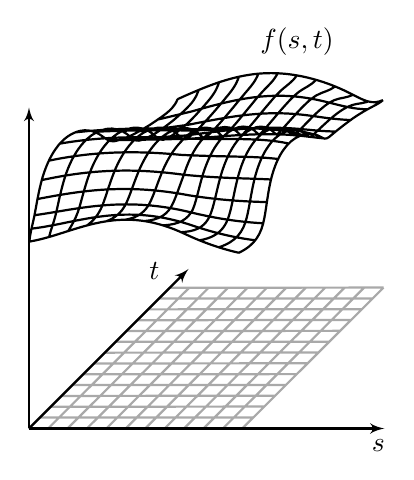
\begin{tikzpicture}[y=0.80pt, x=0.8pt,scale=0.25,yscale=-1, inner sep=0pt, outer sep=0pt]
\usetikzlibrary{arrows}
\begin{scope}[shift={(35.30792,-489.26587)}]% layer1
  \begin{scope}[shift={(-875.37753,2769.7792)}]% g23739
    % path3138
    \path[draw=black,line join=miter,line cap=butt,line width=0.736pt,-latex']
      (840.8022,-1595.0853) -- (840.8022,-2175.0398);

    % path3140
    \path[shift={(5.63871,301.66294)},draw=black,line join=miter,line cap=butt,line
      width=0.800pt,-latex'] (835.1635,-1896.7482) -- (1123.3703,-2184.9551);

    % path3142
    \path[shift={(5.63871,301.66294)},draw=black,line join=miter,line cap=butt,line
      width=0.800pt,-latex'] (835.1635,-1896.7482) -- (1477.1896,-1896.7482);

    % path22889
    \path[draw=black,line join=miter,line cap=butt,line width=0.800pt]
      (1219.8958,-1912.5778) .. controls (1205.3167,-1915.9176) and
      (1190.9914,-1919.9644) .. (1177.0226,-1924.6323) .. controls
      (1158.4596,-1930.8342) and (1140.5258,-1938.1370) .. (1123.3457,-1946.2236) ..
      controls (1110.2347,-1952.3942) and (1096.9616,-1957.7242) ..
      (1083.5085,-1961.8945) .. controls (1083.5085,-1961.8945) and
      (1083.5085,-1961.8945) .. (1083.5085,-1961.8945) .. controls
      (1075.7149,-1964.3101) and (1067.8622,-1966.3387) .. (1059.9473,-1967.9397) ..
      controls (1059.9473,-1967.9397) and (1059.9473,-1967.9397) ..
      (1059.9473,-1967.9397) .. controls (1049.0941,-1970.1347) and
      (1038.1204,-1971.5139) .. (1027.0854,-1972.0473) .. controls
      (1016.0503,-1972.5808) and (1004.9546,-1972.2676) .. (993.8398,-1971.1562) ..
      controls (993.2906,-1971.1012) and (992.7413,-1971.0445) ..
      (992.1920,-1970.9858) .. controls (978.1502,-1969.4842) and
      (964.1093,-1966.7041) .. (950.1335,-1963.1499) .. controls
      (950.1335,-1963.1499) and (950.1335,-1963.1499) .. (950.1335,-1963.1499) ..
      controls (941.3244,-1960.9104) and (932.5441,-1958.3631) ..
      (923.7806,-1955.6657) .. controls (919.8374,-1954.4525) and
      (915.8979,-1953.2108) .. (911.9567,-1951.9592) .. controls
      (900.3543,-1948.2752) and (888.7459,-1944.4891) .. (876.9566,-1941.1021) ..
      controls (865.4444,-1937.7910) and (853.7396,-1934.8514) ..
      (841.6370,-1932.7708)(1249.6091,-1935.1414) .. controls (1229.8179,-1937.6284)
      and (1210.0463,-1941.2804) .. (1190.4670,-1945.9958) .. controls
      (1172.7974,-1950.2575) and (1155.3378,-1955.3871) .. (1138.1503,-1961.1520) ..
      controls (1124.1128,-1965.9738) and (1109.6791,-1970.1512) ..
      (1094.8733,-1973.4264) .. controls (1094.8733,-1973.4264) and
      (1094.8733,-1973.4264) .. (1094.8733,-1973.4264) .. controls
      (1086.3070,-1975.3228) and (1077.6080,-1976.9183) .. (1068.7867,-1978.1817) ..
      controls (1068.7867,-1978.1817) and (1068.7867,-1978.1817) ..
      (1068.7866,-1978.1817) .. controls (1056.6793,-1979.9174) and
      (1044.3460,-1980.9873) .. (1031.8759,-1981.3783) .. controls
      (1019.4057,-1981.7693) and (1006.7993,-1981.4805) .. (994.1419,-1980.5671) ..
      controls (993.5159,-1980.5211) and (992.8899,-1980.4741) ..
      (992.2640,-1980.4254) .. controls (976.2497,-1979.1776) and
      (960.1900,-1976.9304) .. (944.2610,-1974.1371) .. controls
      (934.2224,-1972.3718) and (924.2030,-1970.4140) .. (914.2396,-1968.3984) ..
      controls (909.7611,-1967.4891) and (905.2977,-1966.5726) ..
      (900.8492,-1965.6638) .. controls (887.7402,-1962.9806) and
      (874.7380,-1960.4566) .. (861.8359,-1958.4194) .. controls
      (856.3008,-1957.5536) and (850.8055,-1956.7879) ..
      (845.3414,-1956.1416)(1263.9376,-1965.8417) .. controls (1251.7646,-1966.5184)
      and (1239.4966,-1967.5116) .. (1227.1319,-1968.8618) .. controls
      (1214.7671,-1970.2121) and (1202.3061,-1971.9197) .. (1189.7550,-1973.9852) ..
      controls (1172.6079,-1976.8142) and (1155.3784,-1980.3229) ..
      (1138.0753,-1984.3514) .. controls (1123.4098,-1988.0934) and
      (1108.2043,-1991.3448) .. (1092.5189,-1993.8898) .. controls
      (1092.5189,-1993.8898) and (1092.5189,-1993.8898) .. (1092.5189,-1993.8898) ..
      controls (1083.4492,-1995.3629) and (1074.2056,-1996.6003) ..
      (1064.8096,-1997.5755) .. controls (1064.8096,-1997.5755) and
      (1064.8096,-1997.5755) .. (1064.8096,-1997.5755) .. controls
      (1051.9079,-1998.9178) and (1038.7285,-1999.7096) .. (1025.3872,-1999.9400) ..
      controls (1012.0459,-2000.1704) and (998.5432,-1999.8387) ..
      (985.0038,-1998.9900) .. controls (984.3339,-1998.9470) and
      (983.6641,-1998.9030) .. (982.9945,-1998.8577) .. controls
      (965.8570,-1997.6952) and (948.6992,-1995.7072) .. (931.7982,-1993.2617) ..
      controls (921.1477,-1991.7128) and (910.5488,-1990.0192) ..
      (900.0808,-1988.2822) .. controls (895.3773,-1987.4968) and
      (890.7058,-1986.7084) .. (886.0701,-1985.9269) .. controls
      (874.0490,-1983.8933) and (862.2410,-1982.0180) ..
      (850.7378,-1980.4007)(1270.6245,-2004.0849) .. controls (1268.1158,-2004.1569)
      and (1265.5952,-2004.2333) .. (1263.0616,-2004.3155) .. controls
      (1249.8194,-2004.7373) and (1236.4412,-2005.3028) .. (1222.8491,-2006.1506) ..
      controls (1209.2570,-2006.9985) and (1195.4517,-2008.1296) ..
      (1181.3906,-2009.6062) .. controls (1164.4547,-2011.3904) and
      (1147.2489,-2013.6865) .. (1129.7348,-2016.3980) .. controls
      (1114.6261,-2019.2598) and (1098.9002,-2021.7396) .. (1082.6433,-2023.6468) ..
      controls (1073.2458,-2024.7503) and (1063.6544,-2025.6624) ..
      (1053.8996,-2026.3572) .. controls (1053.8996,-2026.3572) and
      (1053.8995,-2026.3572) .. (1053.8995,-2026.3572) .. controls
      (1040.5024,-2027.3159) and (1026.8087,-2027.8014) .. (1012.9543,-2027.7928) ..
      controls (999.0999,-2027.7828) and (985.0852,-2027.2811) ..
      (971.0648,-2026.3041) .. controls (970.3710,-2026.2551) and
      (969.6774,-2026.2041) .. (968.9841,-2026.1527) .. controls
      (951.2381,-2024.8292) and (933.5223,-2022.7501) .. (916.1929,-2020.1709) ..
      controls (916.1929,-2020.1709) and (916.1929,-2020.1709) ..
      (916.1929,-2020.1709) .. controls (905.2726,-2018.5366) and
      (894.4490,-2016.7449) .. (883.8348,-2014.8557) .. controls
      (879.0662,-2014.0014) and (874.3456,-2013.1332) .. (869.6807,-2012.2559) ..
      controls (865.1275,-2011.3969) and (860.6226,-2010.5459) ..
      (856.1751,-2009.7026)(1278.0447,-2044.9845) .. controls (1270.1643,-2045.4111)
      and (1262.2037,-2045.7343) .. (1254.1029,-2046.0318) .. controls
      (1240.9932,-2046.5045) and (1227.7522,-2046.8906) .. (1214.2538,-2047.3931) ..
      controls (1200.7554,-2047.8955) and (1187.0002,-2048.5156) ..
      (1172.9076,-2049.3687) .. controls (1155.9375,-2050.3997) and
      (1138.5856,-2051.7788) .. (1120.7702,-2053.4673) .. controls
      (1105.3076,-2055.5997) and (1089.1920,-2057.4151) .. (1072.5212,-2058.7407) ..
      controls (1062.8852,-2059.5071) and (1053.0462,-2060.1094) ..
      (1043.0388,-2060.5204) .. controls (1043.0388,-2060.5204) and
      (1043.0388,-2060.5204) .. (1043.0387,-2060.5204) .. controls
      (1015.5491,-2061.6604) and (986.8149,-2061.0702) .. (958.0908,-2058.5767) ..
      controls (957.3801,-2058.5137) and (956.6697,-2058.4502) ..
      (955.9595,-2058.3852) .. controls (937.7823,-2056.7201) and
      (919.6580,-2054.3080) .. (901.9840,-2051.2879) .. controls
      (890.8466,-2049.3757) and (879.8310,-2047.2633) .. (869.0700,-2044.9682) ..
      controls (867.3320,-2044.5955) and (865.6014,-2044.2188) ..
      (863.8785,-2043.8379)(1290.9111,-2081.9588) .. controls (1288.8664,-2082.2123)
      and (1286.8106,-2082.4520) .. (1284.7415,-2082.6803) .. controls
      (1282.0530,-2082.9716) and (1279.3588,-2083.2355) .. (1276.6554,-2083.4755) ..
      controls (1268.0597,-2084.2514) and (1259.3865,-2084.7897) ..
      (1250.5481,-2085.2078) .. controls (1237.3688,-2085.8220) and
      (1224.0605,-2086.1509) .. (1210.4708,-2086.4477) .. controls
      (1196.8812,-2086.7445) and (1183.0105,-2087.0106) .. (1168.7525,-2087.4068) ..
      controls (1168.7525,-2087.4068) and (1168.7525,-2087.4068) ..
      (1168.7525,-2087.4068) .. controls (1151.5838,-2087.8858) and
      (1133.9631,-2088.5626) .. (1115.7684,-2089.4542) .. controls
      (1099.9755,-2090.9914) and (1083.5105,-2092.2501) .. (1066.4690,-2093.0756) ..
      controls (1056.6187,-2093.5525) and (1046.5579,-2093.8834) ..
      (1036.3212,-2094.0415) .. controls (1008.2023,-2094.4879) and
      (978.7830,-2093.3568) .. (949.3021,-2090.3390) .. controls
      (948.5727,-2090.2630) and (947.8435,-2090.1866) .. (947.1146,-2090.1086) ..
      controls (928.4573,-2088.1125) and (909.8240,-2085.3714) ..
      (891.6169,-2081.9274) .. controls (886.6255,-2080.9794) and
      (881.6558,-2079.9857) .. (876.7192,-2078.9454)(1310.0423,-2109.9414) ..
      controls (1302.6874,-2111.5356) and (1295.2796,-2112.7963) ..
      (1287.6942,-2113.8461) .. controls (1284.9758,-2114.2171) and
      (1282.2516,-2114.5530) .. (1279.5179,-2114.8574) .. controls
      (1270.8263,-2115.8376) and (1262.0551,-2116.5047) .. (1253.1147,-2116.9852) ..
      controls (1239.7840,-2117.6923) and (1226.3150,-2117.9679) ..
      (1212.5470,-2118.0949) .. controls (1198.7790,-2118.2219) and
      (1184.7121,-2118.2022) .. (1170.2250,-2118.2317) .. controls
      (1152.7797,-2118.2677) and (1134.8345,-2118.3825) .. (1116.2322,-2118.6509) ..
      controls (1100.1198,-2119.7112) and (1083.3208,-2120.5259) ..
      (1065.9177,-2120.9660) .. controls (1055.8580,-2121.2195) and
      (1045.5783,-2121.3464) .. (1035.1103,-2121.3221) .. controls
      (1035.1103,-2121.3221) and (1035.1103,-2121.3221) .. (1035.1103,-2121.3221) ..
      controls (1006.3570,-2121.2681) and (976.2100,-2119.8156) ..
      (945.8076,-2116.6058) .. controls (945.0555,-2116.5258) and
      (944.3034,-2116.4441) .. (943.5515,-2116.3615) .. controls
      (927.8441,-2114.6366) and (912.1000,-2112.4465) ..
      (896.5237,-2109.7858)(1334.6439,-2125.3158) .. controls (1331.7818,-2126.1473)
      and (1328.9079,-2126.9382) .. (1326.0117,-2127.7017) .. controls
      (1316.2440,-2130.2287) and (1306.4216,-2132.0777) .. (1296.2566,-2133.5140) ..
      controls (1293.5156,-2133.8961) and (1290.7669,-2134.2404) ..
      (1288.0071,-2134.5504) .. controls (1279.2326,-2135.5480) and
      (1270.3629,-2136.2030) .. (1261.3146,-2136.6384) .. controls
      (1247.8232,-2137.2785) and (1234.1729,-2137.4141) .. (1220.2103,-2137.3277) ..
      controls (1206.2476,-2137.2417) and (1191.9728,-2136.9351) ..
      (1177.2586,-2136.6263) .. controls (1159.5391,-2136.2537) and
      (1141.2924,-2135.8818) .. (1122.3321,-2135.6494) .. controls
      (1105.9441,-2136.3241) and (1088.8601,-2136.7966) .. (1071.1410,-2136.9789) ..
      controls (1060.8983,-2137.0831) and (1050.4250,-2137.0886) ..
      (1039.7471,-2136.9786) .. controls (1039.7471,-2136.9786) and
      (1039.7471,-2136.9786) .. (1039.7471,-2136.9786) .. controls
      (1010.4181,-2136.6898) and (979.5760,-2135.2791) .. (948.1881,-2132.4934) ..
      controls (947.4116,-2132.4234) and (946.6350,-2132.3529) ..
      (945.8583,-2132.2813) .. controls (938.7394,-2131.6245) and
      (931.5982,-2130.8972) .. (924.4496,-2130.0998)(1360.8485,-2125.1443) ..
      controls (1352.8911,-2127.3399) and (1344.9422,-2129.1854) ..
      (1336.7541,-2130.9049) .. controls (1327.0042,-2132.9052) and
      (1317.1341,-2134.3593) .. (1306.8920,-2135.4680) .. controls
      (1304.1302,-2135.7616) and (1301.3586,-2136.0224) .. (1298.5743,-2136.2527) ..
      controls (1298.5743,-2136.2527) and (1298.5743,-2136.2527) ..
      (1298.5743,-2136.2527) .. controls (1289.7218,-2136.9980) and
      (1280.7580,-2137.4393) .. (1271.6096,-2137.6737) .. controls
      (1271.6096,-2137.6737) and (1271.6096,-2137.6737) .. (1271.6096,-2137.6737) ..
      controls (1244.3288,-2138.3555) and (1216.3512,-2137.1383) ..
      (1186.6147,-2135.7979) .. controls (1168.7089,-2134.9888) and
      (1150.2801,-2134.1283) .. (1131.1245,-2133.4295) .. controls
      (1114.5892,-2133.7438) and (1097.3663,-2133.9108) .. (1079.4944,-2133.9139) ..
      controls (1069.1631,-2133.9143) and (1058.5963,-2133.8579) ..
      (1047.8138,-2133.7464) .. controls (1019.3347,-2133.4638) and
      (989.3844,-2132.5563) .. (958.6529,-2131.1479)(1377.2011,-2118.8491) ..
      controls (1375.3021,-2119.0266) and (1373.4238,-2119.2086) ..
      (1371.5649,-2119.3957) .. controls (1368.2617,-2119.7298) and
      (1365.0198,-2120.0825) .. (1361.8366,-2120.4584) .. controls
      (1353.1184,-2121.5303) and (1344.4356,-2122.5002) .. (1335.5354,-2123.5158) ..
      controls (1325.3829,-2124.6287) and (1315.1721,-2125.4269) ..
      (1304.6532,-2126.0100) .. controls (1304.6532,-2126.0100) and
      (1304.6532,-2126.0100) .. (1304.6532,-2126.0100) .. controls
      (1301.8167,-2126.1617) and (1298.9751,-2126.2902) .. (1296.1251,-2126.3962) ..
      controls (1296.1251,-2126.3962) and (1296.1251,-2126.3962) ..
      (1296.1251,-2126.3962) .. controls (1287.0643,-2126.7472) and
      (1277.9363,-2126.8725) .. (1268.6583,-2126.8246) .. controls
      (1254.8252,-2126.7456) and (1240.8953,-2126.2622) .. (1226.6958,-2125.4978) ..
      controls (1212.4963,-2124.7335) and (1198.0271,-2123.6908) ..
      (1183.1447,-2122.5572) .. controls (1165.2208,-2121.1883) and
      (1146.8045,-2119.6785) .. (1127.6988,-2118.3228) .. controls
      (1111.2291,-2118.1184) and (1094.1095,-2117.8002) .. (1076.3856,-2117.4509) ..
      controls (1066.1398,-2117.2472) and (1055.6740,-2117.0318) ..
      (1045.0105,-2116.8315) .. controls (1025.3206,-2116.4707) and
      (1004.9783,-2116.0452) .. (984.2252,-2115.7892)(1394.9090,-2131.6385) ..
      controls (1391.9651,-2131.7195) and (1389.1036,-2131.8022) ..
      (1386.3207,-2131.8715) .. controls (1380.7896,-2132.0596) and
      (1375.4247,-2132.3375) .. (1370.1988,-2132.6883) .. controls
      (1366.6988,-2132.9248) and (1363.2623,-2133.1965) .. (1359.8890,-2133.4992) ..
      controls (1350.6544,-2134.3743) and (1341.4882,-2135.2037) ..
      (1332.1847,-2136.0834) .. controls (1321.5738,-2137.0421) and
      (1311.0040,-2137.7003) .. (1300.2250,-2138.1269) .. controls
      (1300.2250,-2138.1269) and (1300.2250,-2138.1269) .. (1300.2250,-2138.1269) ..
      controls (1297.3181,-2138.2364) and (1294.4127,-2138.3220) ..
      (1291.5050,-2138.3837) .. controls (1291.5050,-2138.3837) and
      (1291.5050,-2138.3837) .. (1291.5050,-2138.3837) .. controls
      (1282.2617,-2138.5933) and (1273.0117,-2138.5612) .. (1263.6561,-2138.3257) ..
      controls (1249.7088,-2137.9682) and (1235.7511,-2137.1423) ..
      (1221.5608,-2135.9319) .. controls (1207.3706,-2134.7215) and
      (1192.9474,-2133.1297) .. (1178.1267,-2131.3506) .. controls
      (1160.2743,-2129.2019) and (1141.9435,-2126.7640) .. (1122.9640,-2124.4054) ..
      controls (1106.6887,-2123.3826) and (1089.8087,-2122.2392) ..
      (1072.3919,-2121.1295) .. controls (1062.3231,-2120.4854) and
      (1052.0581,-2119.8507) .. (1041.6260,-2119.2700) .. controls
      (1030.6551,-2118.6647) and (1019.5075,-2118.0840) ..
      (1008.2340,-2117.5903)(1421.8279,-2152.3800) .. controls
      (1411.2790,-2152.7757) and (1401.6264,-2153.6961) .. (1392.6331,-2154.5240) ..
      controls (1387.1279,-2155.0815) and (1381.7337,-2155.7320) ..
      (1376.4383,-2156.4280) .. controls (1372.8919,-2156.8956) and
      (1369.3910,-2157.3860) .. (1365.9406,-2157.8869) .. controls
      (1356.5059,-2159.2937) and (1347.0868,-2160.5336) .. (1337.5764,-2161.6858) ..
      controls (1326.7333,-2162.9588) and (1315.9652,-2163.7969) ..
      (1305.0613,-2164.2843) .. controls (1305.0613,-2164.2843) and
      (1305.0613,-2164.2843) .. (1305.0613,-2164.2843) .. controls
      (1302.1203,-2164.4109) and (1299.1838,-2164.5059) .. (1296.2482,-2164.5694) ..
      controls (1296.2482,-2164.5694) and (1296.2482,-2164.5694) ..
      (1296.2482,-2164.5694) .. controls (1286.9190,-2164.7829) and
      (1277.6129,-2164.6764) .. (1268.2289,-2164.2934) .. controls
      (1254.2426,-2163.7171) and (1240.2756,-2162.5156) .. (1226.0845,-2160.7699) ..
      controls (1211.8933,-2159.0241) and (1197.4776,-2156.7374) ..
      (1182.6673,-2154.1305) .. controls (1164.8203,-2150.9816) and
      (1146.4825,-2147.3403) .. (1127.5169,-2143.6444) .. controls
      (1111.4892,-2141.4794) and (1094.9051,-2139.1575) .. (1077.8426,-2136.8924) ..
      controls (1067.9763,-2135.5794) and (1057.9358,-2134.2821) ..
      (1047.7533,-2133.0596) .. controls (1045.1376,-2132.7469) and
      (1042.5131,-2132.4373) .. (1039.8803,-2132.1320)(1452.5009,-2171.8302) ..
      controls (1446.0032,-2171.8612) and (1439.8532,-2172.2993) ..
      (1433.9152,-2173.0095) .. controls (1423.3011,-2174.2299) and
      (1413.4615,-2176.4700) .. (1403.9487,-2178.6700) .. controls
      (1398.5794,-2179.9531) and (1393.2199,-2181.3074) .. (1387.8828,-2182.6468) ..
      controls (1384.3089,-2183.5446) and (1380.7463,-2184.4375) ..
      (1377.2078,-2185.3026) .. controls (1367.5639,-2187.6796) and
      (1357.8581,-2189.6964) .. (1348.1285,-2191.4086) .. controls
      (1337.0440,-2193.3299) and (1326.0568,-2194.6439) .. (1315.0254,-2195.4437) ..
      controls (1312.0488,-2195.6563) and (1309.0786,-2195.8276) ..
      (1306.1114,-2195.9573) .. controls (1306.1114,-2195.9573) and
      (1306.1114,-2195.9573) .. (1306.1114,-2195.9573) .. controls
      (1296.6876,-2196.3771) and (1287.3034,-2196.3747) .. (1277.8642,-2195.9923) ..
      controls (1263.8030,-2195.4185) and (1249.7459,-2193.9995) ..
      (1235.4437,-2191.7896) .. controls (1221.1416,-2189.5796) and
      (1206.5937,-2186.5823) .. (1191.6341,-2183.0367) .. controls
      (1191.6341,-2183.0367) and (1191.6341,-2183.0367) .. (1191.6341,-2183.0367) ..
      controls (1173.5921,-2178.7536) and (1155.0034,-2173.6320) ..
      (1135.7686,-2168.1859) .. controls (1135.7686,-2168.1859) and
      (1135.7686,-2168.1859) .. (1135.7686,-2168.1859) .. controls
      (1120.0043,-2164.4494) and (1103.7364,-2160.4506) .. (1087.0449,-2156.4833) ..
      controls (1082.5746,-2155.4192) and (1078.0722,-2154.3564) ..
      (1073.5406,-2153.3027)(1480.3175,-2188.3838) .. controls
      (1470.4490,-2183.7703) and (1461.6906,-2183.6492) .. (1452.6188,-2186.2409) ..
      controls (1445.0293,-2188.4030) and (1437.1573,-2192.4517) ..
      (1428.5169,-2196.8506) .. controls (1423.6173,-2199.3521) and
      (1418.4754,-2201.9559) .. (1413.1573,-2204.5082) .. controls
      (1409.5971,-2206.2169) and (1405.9588,-2207.9031) .. (1402.2719,-2209.5249) ..
      controls (1392.2881,-2213.9175) and (1381.9415,-2217.8625) ..
      (1371.5557,-2221.2864) .. controls (1371.5557,-2221.2864) and
      (1371.5557,-2221.2864) .. (1371.5557,-2221.2864) .. controls
      (1359.7405,-2225.1771) and (1347.8761,-2228.3892) .. (1336.0331,-2230.8953) ..
      controls (1332.8350,-2231.5717) and (1329.6391,-2232.1970) ..
      (1326.4444,-2232.7684) .. controls (1316.3095,-2234.5819) and
      (1306.1877,-2235.8441) .. (1296.0512,-2236.5303) .. controls
      (1280.9653,-2237.5508) and (1265.8581,-2237.3055) .. (1250.6114,-2235.6604) ..
      controls (1235.3646,-2234.0152) and (1219.9774,-2230.9741) ..
      (1204.3581,-2226.7182) .. controls (1185.4935,-2221.5770) and
      (1166.2951,-2214.6029) .. (1146.7007,-2206.4105) .. controls
      (1146.7007,-2206.4105) and (1146.7007,-2206.4105) .. (1146.7007,-2206.4105) ..
      controls (1134.3973,-2201.3643) and (1121.9300,-2195.8511) ..
      (1109.3082,-2190.1095)(1219.8958,-1912.5777) .. controls
      (1234.7694,-1919.5872) and (1244.9923,-1928.2002) .. (1252.1376,-1938.5736) ..
      controls (1259.2829,-1948.9471) and (1263.3569,-1961.0846) ..
      (1265.9066,-1974.9133) .. controls (1266.6302,-1978.6363) and
      (1267.2889,-1982.4389) .. (1267.9181,-1986.3030) .. controls
      (1269.5401,-1996.3099) and (1270.9498,-2006.7305) .. (1272.6544,-2017.2656) ..
      controls (1274.3590,-2027.8007) and (1276.3590,-2038.4500) ..
      (1279.0144,-2048.9399) .. controls (1279.1084,-2049.2937) and
      (1279.2036,-2049.6468) .. (1279.2990,-2049.9994) .. controls
      (1279.4892,-2050.7060) and (1279.6814,-2051.4103) .. (1279.8756,-2052.1122) ..
      controls (1281.5052,-2057.9326) and (1283.3040,-2063.5277) ..
      (1285.3042,-2068.8479) .. controls (1288.0786,-2076.2062) and
      (1291.2151,-2083.0479) .. (1294.7588,-2089.2905) .. controls
      (1298.3025,-2095.5331) and (1302.2534,-2101.1769) .. (1306.6095,-2106.1972) ..
      controls (1307.2111,-2106.9020) and (1307.8207,-2107.5872) ..
      (1308.4382,-2108.2530) .. controls (1312.2856,-2112.4353) and
      (1316.3682,-2115.8932) .. (1320.6722,-2118.6764) .. controls
      (1326.7910,-2122.6241) and (1333.3276,-2125.2575) .. (1340.1845,-2126.8651) ..
      controls (1345.4483,-2127.8746) and (1350.5428,-2127.7183) ..
      (1355.4895,-2126.7073) .. controls (1355.6227,-2126.6763) and
      (1355.7554,-2126.6453) .. (1355.8875,-2126.6133) .. controls
      (1358.2249,-2126.0660) and (1360.3723,-2125.3721) .. (1362.3515,-2124.5660) ..
      controls (1364.0763,-2123.8651) and (1365.6792,-2123.0832) ..
      (1367.1761,-2122.2456) .. controls (1369.3018,-2120.9586) and
      (1371.1656,-2120.0119) .. (1372.8275,-2119.4025) .. controls
      (1372.8275,-2119.4025) and (1372.8275,-2119.4025) .. (1372.8275,-2119.4025) ..
      controls (1373.6136,-2119.1145) and (1374.3546,-2118.9018) ..
      (1375.0577,-2118.7634) .. controls (1377.4078,-2118.4469) and
      (1380.0965,-2119.5844) .. (1383.1223,-2121.8731) .. controls
      (1383.9370,-2122.5458) and (1384.7945,-2123.2580) .. (1385.6928,-2124.0076) ..
      controls (1385.6928,-2124.0076) and (1385.6928,-2124.0077) ..
      (1385.6928,-2124.0077) .. controls (1385.8816,-2124.1657) and
      (1386.0724,-2124.3253) .. (1386.2651,-2124.4863) .. controls
      (1390.3612,-2127.9869) and (1395.2807,-2131.9816) .. (1400.8021,-2136.3388) ..
      controls (1406.3235,-2140.6961) and (1412.4461,-2145.4156) ..
      (1418.9355,-2150.2777) .. controls (1421.1292,-2151.8840) and
      (1423.3494,-2153.4828) .. (1425.5920,-2155.0726) .. controls
      (1425.6200,-2155.0926) and (1425.6480,-2155.1116) .. (1425.6750,-2155.1316) ..
      controls (1431.9728,-2159.5474) and (1438.4071,-2163.5529) ..
      (1444.8239,-2167.4241) .. controls (1444.8239,-2167.4241) and
      (1444.8239,-2167.4241) .. (1444.8239,-2167.4241) .. controls
      (1450.0474,-2170.6380) and (1455.4271,-2173.3855) .. (1460.5669,-2176.1574) ..
      controls (1464.7976,-2178.3693) and (1469.1862,-2180.6067) ..
      (1472.9822,-2182.9625) .. controls (1475.8300,-2184.6936) and
      (1478.2485,-2186.6196) .. (1480.3170,-2188.3841)(1183.6478,-1922.4734) ..
      controls (1199.3597,-1927.4714) and (1210.4835,-1934.4608) ..
      (1218.4593,-1943.5403) .. controls (1226.4351,-1952.6197) and
      (1231.2696,-1963.7936) .. (1234.4142,-1976.9730) .. controls
      (1237.1311,-1987.9347) and (1239.1328,-1999.8805) .. (1241.3568,-2012.2771) ..
      controls (1243.5808,-2024.6738) and (1246.0282,-2037.5206) ..
      (1249.3535,-2050.3366) .. controls (1249.3535,-2050.3366) and
      (1249.3535,-2050.3366) .. (1249.3535,-2050.3367) .. controls
      (1249.6507,-2051.4245) and (1249.9518,-2052.5086) .. (1250.2569,-2053.5886) ..
      controls (1250.8949,-2055.8207) and (1251.5547,-2058.0271) ..
      (1252.2383,-2060.2046) .. controls (1255.3357,-2070.0955) and
      (1258.9092,-2079.3819) .. (1263.0880,-2087.8399) .. controls
      (1267.2668,-2096.2978) and (1272.0505,-2103.9279) .. (1277.4659,-2110.6377) ..
      controls (1277.4659,-2110.6377) and (1277.4659,-2110.6377) ..
      (1277.4659,-2110.6377) .. controls (1277.9797,-2111.2838) and
      (1278.4992,-2111.9159) .. (1279.0245,-2112.5341) .. controls
      (1279.1235,-2112.6505) and (1279.2220,-2112.7663) .. (1279.3210,-2112.8817) ..
      controls (1282.8877,-2117.0739) and (1286.6558,-2120.6517) ..
      (1290.6214,-2123.6334) .. controls (1290.6214,-2123.6334) and
      (1290.6214,-2123.6334) .. (1290.6214,-2123.6334) .. controls
      (1297.1643,-2128.5387) and (1304.2051,-2131.8337) .. (1311.6657,-2133.7918) ..
      controls (1317.0734,-2134.9618) and (1322.3056,-2134.8039) ..
      (1327.3851,-2133.5794) .. controls (1327.5220,-2133.5424) and
      (1327.6582,-2133.5044) .. (1327.7937,-2133.4664) .. controls
      (1331.7465,-2132.3783) and (1335.1213,-2130.7738) .. (1338.0053,-2128.7944) ..
      controls (1338.4091,-2128.5151) and (1338.8030,-2128.2289) ..
      (1339.1874,-2127.9362) .. controls (1339.1874,-2127.9362) and
      (1339.1874,-2127.9362) .. (1339.1874,-2127.9362) .. controls
      (1342.2185,-2125.4293) and (1344.5075,-2123.6398) .. (1346.2344,-2122.5729) ..
      controls (1348.0715,-2121.5915) and (1350.1687,-2122.1849) ..
      (1352.5437,-2124.1177) .. controls (1353.3323,-2124.8420) and
      (1354.1855,-2125.6310) .. (1355.1007,-2126.4819) .. controls
      (1356.4914,-2127.8153) and (1358.0140,-2129.2573) .. (1359.6590,-2130.8015) ..
      controls (1363.2243,-2134.2073) and (1367.4295,-2138.1444) ..
      (1372.1503,-2142.4977) .. controls (1372.1503,-2142.4977) and
      (1372.1503,-2142.4977) .. (1372.1503,-2142.4977) .. controls
      (1375.6962,-2145.7701) and (1379.5326,-2149.2747) .. (1383.6081,-2152.9352) ..
      controls (1385.6600,-2154.7203) and (1387.7490,-2156.5070) ..
      (1389.8743,-2158.2915) .. controls (1389.8743,-2158.2915) and
      (1389.8743,-2158.2915) .. (1389.8743,-2158.2915) .. controls
      (1391.9235,-2160.0106) and (1394.0043,-2161.6655) .. (1396.1128,-2163.2658) ..
      controls (1396.1128,-2163.2658) and (1396.1128,-2163.2659) ..
      (1396.1128,-2163.2659) .. controls (1400.0536,-2166.2637) and
      (1404.1152,-2169.0462) .. (1408.2705,-2171.6786) .. controls
      (1408.2705,-2171.6786) and (1408.2705,-2171.6786) .. (1408.2705,-2171.6786) ..
      controls (1413.4301,-2175.0689) and (1419.0354,-2177.5072) ..
      (1424.7517,-2179.4805) .. controls (1429.4081,-2180.8915) and
      (1435.0052,-2181.9087) .. (1440.8224,-2182.6844) .. controls
      (1444.1431,-2183.1052) and (1447.3484,-2183.8581) .. (1450.4546,-2184.8046) ..
      controls (1451.5903,-2185.1499) and (1452.7126,-2185.5213) ..
      (1453.8225,-2185.9127)(1148.8263,-1935.0577) .. controls
      (1169.5400,-1938.6809) and (1182.8172,-1946.2757) .. (1191.5711,-1957.8513) ..
      controls (1196.3817,-1964.1999) and (1199.8329,-1971.7410) ..
      (1202.4012,-1980.4211) .. controls (1205.5060,-1990.6148) and
      (1207.8411,-2001.9868) .. (1210.3214,-2013.9911) .. controls
      (1212.8017,-2025.9953) and (1215.4289,-2038.6311) .. (1218.8624,-2051.4036) ..
      controls (1219.1689,-2052.4875) and (1219.4789,-2053.5691) ..
      (1219.7925,-2054.6478) .. controls (1223.0975,-2065.8905) and
      (1226.9159,-2076.5957) .. (1231.4619,-2086.3914) .. controls
      (1236.0078,-2096.1870) and (1241.2808,-2105.0736) .. (1247.3448,-2112.8770) ..
      controls (1247.3448,-2112.8770) and (1247.3448,-2112.8770) ..
      (1247.3448,-2112.8770) .. controls (1247.9606,-2113.6808) and
      (1248.5848,-2114.4652) .. (1249.2173,-2115.2302) .. controls
      (1250.7520,-2117.1031) and (1252.3239,-2118.8670) .. (1253.9331,-2120.5214) ..
      controls (1258.1277,-2124.8383) and (1262.5659,-2128.4064) ..
      (1267.2404,-2131.2550) .. controls (1271.9150,-2134.1035) and
      (1276.8260,-2136.2329) .. (1281.9498,-2137.7238) .. controls
      (1286.7466,-2138.8907) and (1291.4160,-2138.9943) .. (1295.9704,-2138.1810) ..
      controls (1296.6459,-2138.0609) and (1297.3188,-2137.9206) ..
      (1297.9892,-2137.7609) .. controls (1298.1289,-2137.7229) and
      (1298.2679,-2137.6849) .. (1298.4062,-2137.6459) .. controls
      (1302.0405,-2136.6487) and (1305.1806,-2135.1838) .. (1307.8806,-2133.3460) ..
      controls (1308.5984,-2132.8567) and (1309.2846,-2132.3417) ..
      (1309.9402,-2131.8028) .. controls (1312.9616,-2129.0954) and
      (1315.1707,-2127.0766) .. (1316.7278,-2125.7751) .. controls
      (1318.3745,-2124.5542) and (1320.2585,-2124.9700) .. (1322.3976,-2126.8450) ..
      controls (1323.1168,-2127.5641) and (1323.9028,-2128.3531) ..
      (1324.7534,-2129.2107) .. controls (1324.7534,-2129.2107) and
      (1324.7534,-2129.2107) .. (1324.7534,-2129.2107) .. controls
      (1326.8892,-2131.4379) and (1329.3971,-2133.9941) .. (1332.2395,-2136.8697) ..
      controls (1337.7147,-2142.4031) and (1344.3866,-2149.2282) ..
      (1351.9983,-2157.0368) .. controls (1353.9797,-2159.0003) and
      (1355.9976,-2160.9834) .. (1358.0541,-2162.9863) .. controls
      (1358.0541,-2162.9863) and (1358.0541,-2162.9863) .. (1358.0541,-2162.9863) ..
      controls (1362.7880,-2167.5969) and (1367.7084,-2171.8888) ..
      (1372.8282,-2176.0301) .. controls (1373.8292,-2176.8469) and
      (1374.8393,-2177.6584) .. (1375.8587,-2178.4654) .. controls
      (1380.6710,-2182.4382) and (1386.0351,-2185.4811) .. (1391.7319,-2188.0615) ..
      controls (1391.7319,-2188.0615) and (1391.7319,-2188.0615) ..
      (1391.7319,-2188.0615) .. controls (1391.9401,-2188.1555) and
      (1392.1487,-2188.2495) .. (1392.3577,-2188.3426) .. controls
      (1397.1647,-2190.2377) and (1403.3525,-2191.6885) .. (1410.2293,-2192.9177) ..
      controls (1415.6210,-2193.8224) and (1420.9368,-2195.6477) ..
      (1426.2054,-2198.0289)(1115.6777,-1949.7268) .. controls
      (1121.5458,-1950.0792) and (1126.9022,-1950.7080) .. (1131.7850,-1951.6391) ..
      controls (1131.7850,-1951.6391) and (1131.7850,-1951.6391) ..
      (1131.7850,-1951.6391) .. controls (1142.2322,-1953.7242) and
      (1150.1895,-1957.6121) .. (1156.3206,-1963.2543) .. controls
      (1162.4517,-1968.8964) and (1166.7587,-1976.2951) .. (1169.9180,-1985.3497) ..
      controls (1173.4839,-1995.3292) and (1176.1727,-2006.8575) ..
      (1179.0719,-2019.2470) .. controls (1181.5793,-2029.8956) and
      (1184.2302,-2041.1809) .. (1187.5278,-2052.7048) .. controls
      (1187.8459,-2053.7623) and (1188.1671,-2054.8184) .. (1188.4916,-2055.8727) ..
      controls (1191.9105,-2066.8615) and (1195.8075,-2077.4287) ..
      (1200.4039,-2087.1768) .. controls (1205.0002,-2096.9249) and
      (1210.2956,-2105.8541) .. (1216.3676,-2113.7597) .. controls
      (1216.9843,-2114.5739) and (1217.6092,-2115.3694) .. (1218.2424,-2116.1458) ..
      controls (1223.0201,-2122.0588) and (1228.1515,-2126.9369) ..
      (1233.6378,-2130.7825) .. controls (1239.1240,-2134.6281) and
      (1244.9649,-2137.4419) .. (1251.1270,-2139.3353) .. controls
      (1256.6878,-2140.7746) and (1262.0859,-2140.7829) .. (1267.3387,-2139.5701) ..
      controls (1267.4802,-2139.5331) and (1267.6211,-2139.4951) ..
      (1267.7612,-2139.4565) .. controls (1268.9305,-2139.1436) and
      (1270.0492,-2138.7818) .. (1271.1185,-2138.3736) .. controls
      (1271.1185,-2138.3736) and (1271.1185,-2138.3736) .. (1271.1186,-2138.3736) ..
      controls (1274.3066,-2137.1539) and (1277.0477,-2135.5206) ..
      (1279.3881,-2133.5566) .. controls (1282.4031,-2130.7913) and
      (1284.5816,-2128.7079) .. (1286.0698,-2127.3497) .. controls
      (1287.6390,-2126.0748) and (1289.4402,-2126.4787) .. (1291.4848,-2128.4169) ..
      controls (1291.8273,-2128.7856) and (1292.1862,-2129.1725) ..
      (1292.5615,-2129.5775) .. controls (1292.5615,-2129.5775) and
      (1292.5615,-2129.5775) .. (1292.5615,-2129.5775) .. controls
      (1292.9432,-2129.9916) and (1293.3418,-2130.4246) .. (1293.7570,-2130.8763) ..
      controls (1295.6180,-2132.9693) and (1297.7822,-2135.3510) ..
      (1300.2219,-2138.0250) .. controls (1305.7285,-2144.0412) and
      (1312.5761,-2151.5880) .. (1320.4518,-2160.4966) .. controls
      (1322.4025,-2162.6284) and (1324.3872,-2164.7939) .. (1326.4075,-2166.9968) ..
      controls (1331.9691,-2173.0662) and (1337.7727,-2178.7728) ..
      (1343.8502,-2184.5261) .. controls (1343.8502,-2184.5261) and
      (1343.8502,-2184.5261) .. (1343.8502,-2184.5261) .. controls
      (1344.5612,-2185.2281) and (1345.2845,-2185.9102) .. (1346.0195,-2186.5747) ..
      controls (1350.3203,-2190.4603) and (1355.0109,-2193.7568) ..
      (1359.9749,-2196.8735) .. controls (1364.6758,-2199.5842) and
      (1370.8610,-2202.0038) .. (1377.8133,-2204.5048) .. controls
      (1383.2605,-2206.3274) and (1388.6412,-2209.2956) ..
      (1393.9629,-2213.0487)(1082.7725,-1962.1215) .. controls
      (1083.2801,-1962.1455) and (1083.7839,-1962.1725) .. (1084.2839,-1962.2015) ..
      controls (1098.0062,-1962.9907) and (1108.8447,-1965.4959) ..
      (1117.3433,-1970.1250) .. controls (1125.8418,-1974.7542) and
      (1132.0101,-1981.5098) .. (1136.6435,-1990.5360) .. controls
      (1136.8016,-1990.9135) and (1136.9571,-1991.2951) .. (1137.1101,-1991.6807) ..
      controls (1140.4678,-1999.9693) and (1143.1127,-2009.7288) ..
      (1145.8802,-2020.3987) .. controls (1148.6477,-2031.0686) and
      (1151.5405,-2042.6481) .. (1155.1849,-2054.6234) .. controls
      (1155.1849,-2054.6234) and (1155.1849,-2054.6234) .. (1155.1849,-2054.6234) ..
      controls (1155.5097,-2055.6384) and (1155.8376,-2056.6529) ..
      (1156.1687,-2057.6664) .. controls (1159.7610,-2068.5474) and
      (1163.8559,-2079.0830) .. (1168.6927,-2088.8254) .. controls
      (1168.6927,-2088.8254) and (1168.6927,-2088.8254) .. (1168.6927,-2088.8254) ..
      controls (1173.2636,-2098.0003) and (1178.4821,-2106.4735) ..
      (1184.4219,-2114.0409) .. controls (1184.4219,-2114.0409) and
      (1184.4219,-2114.0409) .. (1184.4219,-2114.0409) .. controls
      (1185.0438,-2114.8448) and (1185.6738,-2115.6304) .. (1186.3119,-2116.3976) ..
      controls (1191.1277,-2122.2401) and (1196.2921,-2127.0804) ..
      (1201.8096,-2130.9068) .. controls (1207.3270,-2134.7332) and
      (1213.1976,-2137.5462) .. (1219.3896,-2139.4448) .. controls
      (1224.9774,-2140.8869) and (1230.4001,-2140.8967) .. (1235.6740,-2139.6739) ..
      controls (1235.8162,-2139.6359) and (1235.9576,-2139.5979) ..
      (1236.0983,-2139.5593) .. controls (1240.7768,-2138.3018) and
      (1244.6374,-2136.2540) .. (1247.7785,-2133.6038) .. controls
      (1247.7785,-2133.6038) and (1247.7785,-2133.6038) .. (1247.7785,-2133.6038) ..
      controls (1250.8085,-2130.8086) and (1252.9967,-2128.6995) ..
      (1254.4826,-2127.3280) .. controls (1256.0486,-2126.0413) and
      (1257.8461,-2126.4600) .. (1259.8807,-2128.4555) .. controls
      (1260.5701,-2129.2204) and (1261.3270,-2130.0626) .. (1262.1490,-2130.9821) ..
      controls (1262.1490,-2130.9821) and (1262.1490,-2130.9821) ..
      (1262.1490,-2130.9821) .. controls (1262.7360,-2131.6603) and
      (1263.3530,-2132.3690) .. (1263.9992,-2133.1085) .. controls
      (1267.0028,-2136.5511) and (1270.6265,-2140.6665) .. (1274.7737,-2145.4651) ..
      controls (1278.9208,-2150.2637) and (1283.5905,-2155.7457) ..
      (1288.6822,-2161.8791) .. controls (1290.6170,-2164.1338) and
      (1292.5832,-2166.4331) .. (1294.5814,-2168.7833) .. controls
      (1295.9761,-2170.4259) and (1297.3850,-2172.0514) .. (1298.8081,-2173.6680) ..
      controls (1298.8081,-2173.6680) and (1298.8081,-2173.6680) ..
      (1298.8081,-2173.6680) .. controls (1302.9921,-2178.4301) and
      (1307.2962,-2183.1138) .. (1311.7314,-2187.9283) .. controls
      (1312.0116,-2188.2449) and (1312.2938,-2188.5588) .. (1312.5777,-2188.8701) ..
      controls (1317.1261,-2193.8492) and (1322.1344,-2198.1709) ..
      (1327.4340,-2202.5087) .. controls (1331.9891,-2206.0263) and
      (1337.9649,-2209.4454) .. (1344.5516,-2213.2907) .. controls
      (1349.6838,-2216.0738) and (1354.6861,-2220.1041) ..
      (1359.5259,-2225.0133)(1049.1391,-1969.8506) .. controls
      (1055.6643,-1970.3843) and (1061.5586,-1971.3265) .. (1066.8482,-1972.7470) ..
      controls (1066.8482,-1972.7470) and (1066.8482,-1972.7470) ..
      (1066.8482,-1972.7470) .. controls (1078.5044,-1975.8796) and
      (1087.1768,-1981.3875) .. (1093.6591,-1989.7724) .. controls
      (1093.6591,-1989.7724) and (1093.6591,-1989.7724) .. (1093.6591,-1989.7724) ..
      controls (1095.8693,-1992.6244) and (1097.8330,-1995.8051) ..
      (1099.5938,-1999.3211) .. controls (1103.3185,-2006.6593) and
      (1106.5547,-2015.0847) .. (1109.8940,-2024.2681) .. controls
      (1113.2334,-2033.4516) and (1116.6795,-2043.3914) .. (1120.7179,-2053.7344) ..
      controls (1120.7179,-2053.7344) and (1120.7179,-2053.7344) ..
      (1120.7179,-2053.7344) .. controls (1121.0882,-2054.9194) and
      (1121.4660,-2056.1105) .. (1121.8521,-2057.3071) .. controls
      (1122.1793,-2058.2704) and (1122.5095,-2059.2339) .. (1122.8431,-2060.1972) ..
      controls (1126.3564,-2070.2374) and (1130.3474,-2080.0319) ..
      (1135.0330,-2089.1580) .. controls (1139.7187,-2098.2840) and
      (1145.0995,-2106.7411) .. (1151.2587,-2114.2875) .. controls
      (1151.8842,-2115.0658) and (1152.5179,-2115.8264) .. (1153.1598,-2116.5690) ..
      controls (1159.9756,-2124.5244) and (1167.5010,-2130.5370) ..
      (1175.7319,-2134.6133) .. controls (1175.7319,-2134.6133) and
      (1175.7319,-2134.6134) .. (1175.7319,-2134.6134) .. controls
      (1179.2101,-2136.3322) and (1182.8098,-2137.7124) .. (1186.5229,-2138.7775) ..
      controls (1192.1714,-2140.1265) and (1197.6569,-2140.0525) ..
      (1202.9952,-2138.7515) .. controls (1203.1391,-2138.7115) and
      (1203.2822,-2138.6715) .. (1203.4247,-2138.6305) .. controls
      (1208.1609,-2137.3029) and (1212.0792,-2135.1894) .. (1215.2763,-2132.4786) ..
      controls (1218.3633,-2129.6215) and (1220.6066,-2127.4580) ..
      (1222.1433,-2126.0442) .. controls (1223.7646,-2124.7114) and
      (1225.6132,-2125.0991) .. (1227.6900,-2127.0839) .. controls
      (1228.3925,-2127.8453) and (1229.1615,-2128.6858) .. (1229.9946,-2129.6059) ..
      controls (1233.0622,-2133.1066) and (1236.9164,-2137.4507) ..
      (1241.4190,-2142.6809) .. controls (1245.9217,-2147.9111) and
      (1251.0714,-2154.0274) .. (1256.7136,-2161.0096) .. controls
      (1258.6495,-2163.3306) and (1260.6145,-2165.7053) .. (1262.6084,-2168.1413) ..
      controls (1265.9243,-2172.1989) and (1269.3123,-2176.1953) ..
      (1272.7720,-2180.2561) .. controls (1275.0376,-2182.9172) and
      (1277.3325,-2185.6063) .. (1279.6587,-2188.3595) .. controls
      (1279.6588,-2188.3595) and (1279.6588,-2188.3595) .. (1279.6588,-2188.3595) ..
      controls (1284.3755,-2194.1534) and (1289.5961,-2199.3098) ..
      (1295.0936,-2204.7672) .. controls (1299.5484,-2209.0158) and
      (1305.2918,-2213.3825) .. (1311.4017,-2218.5242) .. controls
      (1316.1142,-2222.2238) and (1320.6150,-2227.1975) ..
      (1324.8326,-2233.0533)(1014.8855,-1972.2969) .. controls
      (1025.8322,-1974.2319) and (1034.9797,-1977.5523) .. (1042.3842,-1982.7810) ..
      controls (1049.7886,-1988.0096) and (1055.4646,-1995.1527) ..
      (1059.9249,-2004.4776) .. controls (1060.3435,-2005.3392) and
      (1060.7572,-2006.2140) .. (1061.1670,-2007.1015) .. controls
      (1061.1670,-2007.1015) and (1061.1670,-2007.1015) .. (1061.1670,-2007.1015) ..
      controls (1066.2184,-2018.0749) and (1070.6704,-2031.0464) ..
      (1076.0295,-2045.1251) .. controls (1078.0859,-2050.5071) and
      (1080.2747,-2056.0490) .. (1082.6642,-2061.6958) .. controls
      (1083.0696,-2062.6092) and (1083.4780,-2063.5220) .. (1083.8896,-2064.4339) ..
      controls (1088.0786,-2073.6342) and (1092.7031,-2082.5289) ..
      (1097.9470,-2090.7840) .. controls (1103.1909,-2099.0391) and
      (1109.0554,-2106.6530) .. (1115.6206,-2113.4201) .. controls
      (1115.6207,-2113.4201) and (1115.6207,-2113.4202) .. (1115.6207,-2113.4202) ..
      controls (1116.0098,-2113.8873) and (1116.4020,-2114.3510) ..
      (1116.7975,-2114.8112) .. controls (1117.4265,-2115.5557) and
      (1118.0639,-2116.2829) .. (1118.7097,-2116.9926) .. controls
      (1123.5841,-2122.3956) and (1128.8228,-2126.8508) .. (1134.4336,-2130.3292) ..
      controls (1140.0445,-2133.8075) and (1146.0277,-2136.3092) ..
      (1152.3501,-2137.9191) .. controls (1158.0553,-2139.1012) and
      (1163.6103,-2138.8678) .. (1169.0309,-2137.4122) .. controls
      (1169.1770,-2137.3682) and (1169.3224,-2137.3242) .. (1169.4670,-2137.2788) ..
      controls (1174.2775,-2135.8135) and (1178.2802,-2133.5662) ..
      (1181.5712,-2130.7272) .. controls (1181.5712,-2130.7272) and
      (1181.5712,-2130.7272) .. (1181.5712,-2130.7272) .. controls
      (1183.4423,-2128.9708) and (1185.0268,-2127.4553) .. (1186.3486,-2126.1936) ..
      controls (1186.3486,-2126.1935) and (1186.3486,-2126.1935) ..
      (1186.3486,-2126.1935) .. controls (1187.2795,-2125.3089) and
      (1188.0809,-2124.5490) .. (1188.7637,-2123.9177) .. controls
      (1190.5165,-2122.4553) and (1192.4976,-2122.7214) .. (1194.7013,-2124.5953) ..
      controls (1195.4433,-2125.3210) and (1196.2511,-2126.1273) ..
      (1197.1217,-2127.0147) .. controls (1200.3265,-2130.3948) and
      (1204.3033,-2134.6404) .. (1208.9051,-2139.8073) .. controls
      (1213.5069,-2144.9742) and (1218.7326,-2151.0626) .. (1224.4160,-2158.0626) ..
      controls (1226.3657,-2160.3915) and (1228.3411,-2162.7810) ..
      (1230.3420,-2165.2400) .. controls (1230.3420,-2165.2400) and
      (1230.3420,-2165.2400) .. (1230.3421,-2165.2400) .. controls
      (1235.8522,-2172.0222) and (1241.5326,-2178.7180) .. (1247.3960,-2185.9700) ..
      controls (1247.3960,-2185.9700) and (1247.3960,-2185.9700) ..
      (1247.3960,-2185.9700) .. controls (1252.1099,-2192.0034) and
      (1257.2984,-2197.5550) .. (1262.7137,-2203.6854) .. controls
      (1267.1123,-2208.5240) and (1272.6494,-2213.6967) .. (1278.2893,-2219.9800) ..
      controls (1282.5829,-2224.4770) and (1286.5820,-2230.2459) ..
      (1290.1820,-2236.8653)(980.3422,-1969.4289) .. controls (985.0577,-1971.1769)
      and (989.4742,-1973.2561) .. (993.5301,-1975.7579) .. controls
      (994.0938,-1976.1058) and (994.6507,-1976.4618) .. (995.2006,-1976.8261) ..
      controls (1000.2319,-1980.1578) and (1004.6626,-1984.1937) ..
      (1008.5138,-1989.0918) .. controls (1012.3651,-1993.9899) and
      (1015.6393,-1999.7510) .. (1018.4631,-2006.4703) .. controls
      (1021.9454,-2014.5877) and (1025.2095,-2023.6674) .. (1028.7821,-2033.4259) ..
      controls (1032.3546,-2043.1844) and (1036.2420,-2053.6194) ..
      (1040.9104,-2064.3875) .. controls (1040.9104,-2064.3876) and
      (1040.9104,-2064.3876) .. (1040.9104,-2064.3876) .. controls
      (1041.1632,-2064.9437) and (1041.4172,-2065.4995) .. (1041.6725,-2066.0548) ..
      controls (1041.6725,-2066.0548) and (1041.6725,-2066.0548) ..
      (1041.6725,-2066.0548) .. controls (1041.8347,-2066.4084) and
      (1041.9973,-2066.7618) .. (1042.1605,-2067.1150) .. controls
      (1048.6621,-2081.0716) and (1056.2558,-2094.2387) .. (1065.4825,-2105.5849) ..
      controls (1065.4825,-2105.5849) and (1065.4825,-2105.5849) ..
      (1065.4825,-2105.5849) .. controls (1068.7781,-2109.6284) and
      (1072.2788,-2113.4460) .. (1075.9922,-2117.0112) .. controls
      (1075.9922,-2117.0112) and (1075.9922,-2117.0112) .. (1075.9922,-2117.0112) ..
      controls (1076.7086,-2117.7130) and (1077.4332,-2118.3970) ..
      (1078.1661,-2119.0629) .. controls (1083.7058,-2124.1316) and
      (1089.6016,-2128.2207) .. (1095.8660,-2131.3064) .. controls
      (1102.1303,-2134.3921) and (1108.7636,-2136.4740) .. (1115.7331,-2137.6391) ..
      controls (1119.8540,-2138.1519) and (1123.9097,-2138.0505) ..
      (1127.9042,-2137.3827) .. controls (1129.8408,-2137.1092) and
      (1131.7627,-2136.6818) .. (1133.6704,-2136.1100) .. controls
      (1133.8197,-2136.0610) and (1133.9682,-2136.0110) .. (1134.1160,-2135.9602) ..
      controls (1139.0319,-2134.3121) and (1143.1524,-2131.8781) ..
      (1146.5709,-2128.8471) .. controls (1149.8842,-2125.6630) and
      (1152.3737,-2123.1715) .. (1154.1679,-2121.4344) .. controls
      (1156.0711,-2119.7476) and (1158.2111,-2119.7849) .. (1160.5728,-2121.4344) ..
      controls (1161.3643,-2122.0884) and (1162.2213,-2122.8231) ..
      (1163.1405,-2123.6394) .. controls (1163.1405,-2123.6394) and
      (1163.1405,-2123.6394) .. (1163.1405,-2123.6394) .. controls
      (1167.3579,-2127.5294) and (1172.7661,-2132.7816) .. (1179.0545,-2139.5180) ..
      controls (1179.0545,-2139.5180) and (1179.0545,-2139.5180) ..
      (1179.0545,-2139.5180) .. controls (1182.8619,-2143.5875) and
      (1186.9853,-2148.1962) .. (1191.3476,-2153.3411) .. controls
      (1193.3341,-2155.6135) and (1195.3427,-2157.9522) .. (1197.3729,-2160.3668) ..
      controls (1197.3729,-2160.3668) and (1197.3729,-2160.3669) ..
      (1197.3730,-2160.3669) .. controls (1202.9658,-2167.0273) and
      (1208.7010,-2173.6686) .. (1214.5928,-2180.9947) .. controls
      (1219.3359,-2187.0843) and (1224.5191,-2192.8245) .. (1229.8782,-2199.3852) ..
      controls (1234.2406,-2204.6082) and (1239.6067,-2210.3540) ..
      (1244.8360,-2217.5048) .. controls (1248.7641,-2222.5971) and
      (1252.3217,-2228.9571) .. (1255.3781,-2236.1345)(945.8561,-1962.0426) ..
      controls (947.0869,-1962.9660) and (948.3079,-1963.9223) ..
      (949.5120,-1964.9168) .. controls (955.0286,-1969.4721) and
      (960.1569,-1974.8293) .. (964.6043,-1981.4015) .. controls
      (969.0517,-1987.9736) and (972.8280,-1995.7658) .. (976.0359,-2005.0485) ..
      controls (976.5048,-2006.3672) and (976.9725,-2007.7057) ..
      (977.4406,-2009.0632) .. controls (977.4406,-2009.0632) and
      (977.4406,-2009.0632) .. (977.4406,-2009.0632) .. controls
      (977.7219,-2009.8809) and (978.0035,-2010.7054) .. (978.2857,-2011.5366) ..
      controls (980.9495,-2019.3948) and (983.6523,-2027.8602) ..
      (986.7032,-2036.7681) .. controls (989.7542,-2045.6760) and
      (993.1569,-2055.0253) .. (997.1985,-2064.6072) .. controls
      (997.6070,-2065.5316) and (998.0192,-2066.4547) .. (998.4354,-2067.3763) ..
      controls (1002.8094,-2076.9818) and (1007.7228,-2086.2065) ..
      (1013.3648,-2094.7090) .. controls (1019.0067,-2103.2115) and
      (1025.3794,-2110.9893) .. (1032.5681,-2117.8171) .. controls
      (1032.5681,-2117.8171) and (1032.5681,-2117.8171) .. (1032.5681,-2117.8171) ..
      controls (1033.2967,-2118.5232) and (1034.0339,-2119.2111) ..
      (1034.7798,-2119.8809) .. controls (1034.8588,-2119.9529) and
      (1034.9387,-2120.0242) .. (1035.0182,-2120.0956) .. controls
      (1035.0182,-2120.0956) and (1035.0182,-2120.0956) .. (1035.0182,-2120.0956) ..
      controls (1040.5836,-2125.0987) and (1046.5170,-2129.1432) ..
      (1052.8360,-2132.1968) .. controls (1059.1551,-2135.2504) and
      (1065.8601,-2137.3126) .. (1072.9226,-2138.4549) .. controls
      (1073.0176,-2138.4699) and (1073.1120,-2138.4849) .. (1073.2068,-2138.4999) ..
      controls (1079.6831,-2139.2536) and (1086.0386,-2138.5499) ..
      (1092.2883,-2136.5701) .. controls (1092.4567,-2136.5121) and
      (1092.6243,-2136.4537) .. (1092.7913,-2136.3944) .. controls
      (1098.3450,-2134.4574) and (1103.1139,-2131.6945) .. (1107.1829,-2128.2924) ..
      controls (1111.1601,-2124.7292) and (1114.3153,-2121.8156) ..
      (1116.7596,-2119.6224) .. controls (1119.2164,-2117.5686) and
      (1121.8678,-2117.0030) .. (1124.6816,-2117.8524) .. controls
      (1124.8338,-2117.9194) and (1124.9867,-2117.9928) .. (1125.1405,-2118.0716) ..
      controls (1125.9949,-2118.6210) and (1126.9136,-2119.2502) ..
      (1127.8935,-2119.9604) .. controls (1131.4978,-2122.6923) and
      (1135.8502,-2126.2883) .. (1140.7862,-2130.8372) .. controls
      (1145.7221,-2135.3862) and (1151.2406,-2140.8885) .. (1157.1527,-2147.3604) ..
      controls (1159.1802,-2149.5108) and (1161.2268,-2151.7305) ..
      (1163.2917,-2154.0302) .. controls (1168.9812,-2160.3721) and
      (1174.7891,-2166.7318) .. (1180.7274,-2173.8661) .. controls
      (1180.7274,-2173.8661) and (1180.7274,-2173.8661) .. (1180.7274,-2173.8661) ..
      controls (1184.8975,-2179.0341) and (1189.3828,-2184.0032) ..
      (1193.9953,-2189.6029) .. controls (1194.6755,-2190.4279) and
      (1195.3584,-2191.2668) .. (1196.0435,-2192.1225) .. controls
      (1200.3920,-2197.4473) and (1205.6517,-2203.4337) .. (1210.5883,-2211.0549) ..
      controls (1214.2553,-2216.4560) and (1217.4880,-2223.1357) ..
      (1220.1332,-2230.6206)(911.5827,-1951.8443) .. controls (911.6484,-1951.9521)
      and (911.7143,-1952.0600) .. (911.7804,-1952.1681) .. controls
      (913.8708,-1955.5899) and (916.0980,-1959.1500) .. (918.2954,-1962.9799) ..
      controls (920.7404,-1967.2345) and (923.1467,-1971.8169) ..
      (925.3857,-1976.8776) .. controls (927.6247,-1981.9382) and
      (929.6981,-1987.4775) .. (931.5761,-1993.6094) .. controls
      (932.2615,-1995.8446) and (932.9234,-1998.1570) .. (933.5634,-2000.5505) ..
      controls (936.0575,-2009.5244) and (938.6230,-2019.2535) ..
      (941.6481,-2029.5527) .. controls (944.6732,-2039.8519) and
      (948.1662,-2050.7190) .. (952.5320,-2061.8768) .. controls
      (952.5320,-2061.8768) and (952.5320,-2061.8768) .. (952.5320,-2061.8768) ..
      controls (952.9190,-2062.8220) and (953.3102,-2063.7659) ..
      (953.7057,-2064.7084) .. controls (953.7492,-2064.8111) and
      (953.7927,-2064.9138) .. (953.8363,-2065.0164) .. controls
      (953.8363,-2065.0164) and (953.8363,-2065.0164) .. (953.8363,-2065.0164) ..
      controls (954.2627,-2066.0220) and (954.6954,-2067.0236) ..
      (955.1346,-2068.0210) .. controls (955.1346,-2068.0210) and
      (955.1346,-2068.0210) .. (955.1346,-2068.0210) .. controls
      (959.1703,-2077.1959) and (963.7425,-2086.0056) .. (969.0106,-2094.1712) ..
      controls (974.2786,-2102.3367) and (980.2444,-2109.8561) ..
      (986.9885,-2116.5311) .. controls (987.7128,-2117.2614) and
      (988.4463,-2117.9739) .. (989.1891,-2118.6682) .. controls
      (994.8061,-2123.9546) and (1000.8410,-2128.2563) .. (1007.3217,-2131.5197) ..
      controls (1013.8025,-2134.7832) and (1020.7297,-2137.0077) ..
      (1028.0795,-2138.2479) .. controls (1034.1073,-2139.0237) and
      (1040.0739,-2138.5738) .. (1045.9911,-2137.0086) .. controls
      (1045.9911,-2137.0086) and (1045.9911,-2137.0086) .. (1045.9911,-2137.0086) ..
      controls (1046.5800,-2136.8528) and (1047.1684,-2136.6861) ..
      (1047.7563,-2136.5087) .. controls (1047.9311,-2136.4517) and
      (1048.1052,-2136.3934) .. (1048.2787,-2136.3346) .. controls
      (1054.0485,-2134.4152) and (1059.0740,-2131.6297) .. (1063.4279,-2128.1484) ..
      controls (1067.6965,-2124.5044) and (1071.1718,-2121.4478) ..
      (1073.9436,-2119.0525) .. controls (1074.7427,-2118.4055) and
      (1075.5588,-2117.8748) .. (1076.3903,-2117.4600) .. controls
      (1076.3903,-2117.4600) and (1076.3903,-2117.4600) .. (1076.3903,-2117.4600) ..
      controls (1078.6571,-2116.3320) and (1081.0396,-2116.0629) ..
      (1083.5191,-2116.6186) .. controls (1084.6345,-2116.9952) and
      (1085.8114,-2117.4461) .. (1087.0459,-2117.9735) .. controls
      (1091.5813,-2120.0380) and (1096.8196,-2122.9049) .. (1102.5676,-2126.7032) ..
      controls (1108.3156,-2130.5015) and (1114.5724,-2135.2316) ..
      (1121.1097,-2140.9535) .. controls (1123.3509,-2142.8472) and
      (1125.5975,-2144.8124) .. (1127.8474,-2146.8618) .. controls
      (1127.8474,-2146.8618) and (1127.8474,-2146.8618) .. (1127.8474,-2146.8618) ..
      controls (1128.1913,-2147.1750) and (1128.5351,-2147.4882) ..
      (1128.8790,-2147.8018) .. controls (1134.3679,-2153.3201) and
      (1139.9293,-2158.8954) .. (1145.5739,-2165.2014) .. controls
      (1150.3889,-2170.7549) and (1155.5956,-2176.0671) .. (1160.8988,-2182.4714) ..
      controls (1165.2223,-2187.5843) and (1170.4274,-2193.4280) ..
      (1175.2075,-2201.0464) .. controls (1178.7359,-2206.4204) and
      (1181.7875,-2213.1023) .. (1184.1914,-2220.6052)(877.1761,-1941.1691) ..
      controls (878.5369,-1947.4458) and (880.6022,-1953.5710) ..
      (882.7346,-1960.1414) .. controls (884.8670,-1966.7119) and
      (887.0732,-1973.7272) .. (889.0847,-1981.6149) .. controls
      (890.0925,-1985.5800) and (891.0580,-1989.7542) .. (891.9764,-1994.1734) ..
      controls (892.3277,-1995.7868) and (892.6832,-1997.4225) ..
      (893.0446,-1999.0802) .. controls (896.1006,-2013.0239) and
      (899.5041,-2028.5474) .. (904.4859,-2045.0694) .. controls
      (905.5872,-2048.7181) and (906.7694,-2052.4113) .. (908.0469,-2056.1392) ..
      controls (908.3904,-2057.0988) and (908.7384,-2058.0577) ..
      (909.0909,-2059.0157) .. controls (912.7981,-2068.9997) and
      (917.1064,-2078.6887) .. (922.2302,-2087.7284) .. controls
      (927.3540,-2096.7682) and (933.2964,-2105.1557) .. (940.1821,-2112.6208) ..
      controls (940.8798,-2113.3892) and (941.5873,-2114.1405) ..
      (942.3047,-2114.8744) .. controls (942.7194,-2115.3015) and
      (943.1368,-2115.7231) .. (943.5568,-2116.1391) .. controls
      (943.5568,-2116.1391) and (943.5568,-2116.1391) .. (943.5568,-2116.1391) ..
      controls (944.2910,-2116.8670) and (945.0337,-2117.5777) ..
      (945.7851,-2118.2711) .. controls (950.8083,-2122.9055) and
      (956.2120,-2126.7591) .. (962.0222,-2129.7832) .. controls
      (967.8324,-2132.8074) and (974.0493,-2135.0017) .. (980.6622,-2136.3864) ..
      controls (987.3255,-2137.5227) and (993.9875,-2137.1683) ..
      (1000.6641,-2135.4325) .. controls (1000.8439,-2135.3815) and
      (1001.0231,-2135.3293) .. (1001.2017,-2135.2765) .. controls
      (1007.1440,-2133.5554) and (1012.4151,-2130.9161) .. (1017.0671,-2127.4998) ..
      controls (1021.6423,-2123.9234) and (1025.4786,-2120.8327) ..
      (1028.6306,-2118.3068) .. controls (1032.0180,-2115.7577) and
      (1035.6510,-2114.7095) .. (1039.4555,-2115.1305) .. controls
      (1040.2255,-2115.2978) and (1041.0187,-2115.4906) .. (1041.8343,-2115.7095) ..
      controls (1041.8343,-2115.7095) and (1041.8343,-2115.7095) ..
      (1041.8343,-2115.7095) .. controls (1042.3368,-2115.8449) and
      (1042.8478,-2115.9903) .. (1043.3670,-2116.1460) .. controls
      (1047.8877,-2117.6192) and (1052.9741,-2119.6796) .. (1058.4859,-2122.4424) ..
      controls (1063.9976,-2125.2052) and (1069.9341,-2128.6708) ..
      (1076.1305,-2132.9041) .. controls (1076.1305,-2132.9041) and
      (1076.1305,-2132.9041) .. (1076.1305,-2132.9042) .. controls
      (1077.4369,-2133.7954) and (1078.7548,-2134.7205) .. (1080.0827,-2135.6798) ..
      controls (1082.4719,-2137.3378) and (1084.8654,-2139.0610) ..
      (1087.2609,-2140.8625) .. controls (1093.8658,-2145.8210) and
      (1100.4622,-2150.7569) .. (1107.0190,-2156.5110) .. controls
      (1107.0190,-2156.5110) and (1107.0190,-2156.5110) .. (1107.0190,-2156.5110) ..
      controls (1112.3073,-2161.3104) and (1117.9108,-2165.8363) ..
      (1123.5003,-2171.4775) .. controls (1128.0570,-2175.9457) and
      (1133.4664,-2181.1561) .. (1138.3634,-2188.2108) .. controls
      (1141.5685,-2192.6107) and (1144.3525,-2198.0907) .. (1146.5834,-2204.3146) ..
      controls (1146.8618,-2205.0997) and (1147.1319,-2205.8963) ..
      (1147.3935,-2206.7037)(841.6365,-1932.7745) .. controls (842.0731,-1940.1769)
      and (843.3201,-1946.8692) .. (844.7879,-1953.6390) .. controls
      (846.2557,-1960.4089) and (847.9471,-1967.2544) .. (849.5690,-1974.7432) ..
      controls (850.4491,-1978.8528) and (851.3001,-1983.1463) ..
      (852.1030,-1987.6882) .. controls (853.2619,-1993.9788) and
      (854.4528,-2000.6420) .. (855.7865,-2007.6730) .. controls
      (857.1203,-2014.7040) and (858.5991,-2022.1017) .. (860.3733,-2029.8135) ..
      controls (861.7203,-2035.6876) and (863.2430,-2041.7313) ..
      (865.0138,-2047.9060) .. controls (865.2984,-2048.8594) and
      (865.5874,-2049.8133) .. (865.8810,-2050.7674) .. controls
      (865.9938,-2051.1308) and (866.1073,-2051.4939) .. (866.2217,-2051.8569) ..
      controls (871.4029,-2068.2527) and (878.1983,-2084.2165) ..
      (887.5977,-2098.1396) .. controls (889.3763,-2100.7720) and
      (891.2482,-2103.3315) .. (893.2174,-2105.8095) .. controls
      (893.8561,-2106.6230) and (894.5051,-2107.4209) .. (895.1648,-2108.2030) ..
      controls (900.1549,-2114.1623) and (905.6572,-2119.2534) ..
      (911.7390,-2123.3468) .. controls (917.8208,-2127.4402) and
      (924.4828,-2130.5348) .. (931.7320,-2132.6043) .. controls
      (938.1292,-2134.1908) and (944.6217,-2134.3744) .. (951.2251,-2133.1916) ..
      controls (951.2251,-2133.1916) and (951.2251,-2133.1916) ..
      (951.2251,-2133.1916) .. controls (951.3685,-2133.1656) and
      (951.5119,-2133.1396) .. (951.6553,-2133.1126) .. controls
      (951.8370,-2133.0746) and (952.0182,-2133.0346) .. (952.1990,-2132.9948) ..
      controls (952.8748,-2132.8484) and (953.5438,-2132.6900) ..
      (954.2059,-2132.5196) .. controls (959.4276,-2131.1688) and
      (964.2087,-2129.0642) .. (968.5659,-2126.2780) .. controls
      (968.5659,-2126.2780) and (968.5659,-2126.2780) .. (968.5659,-2126.2780) ..
      controls (973.4096,-2122.9876) and (977.5991,-2120.0434) ..
      (981.1381,-2117.5325) .. controls (984.9497,-2114.9950) and
      (989.0216,-2113.7863) .. (993.2547,-2113.9335) .. controls
      (994.6340,-2114.1167) and (996.0726,-2114.3568) .. (997.5670,-2114.6574) ..
      controls (1003.0522,-2115.8931) and (1009.2151,-2117.7227) ..
      (1015.8719,-2120.3298) .. controls (1022.5287,-2122.9370) and
      (1029.6788,-2126.3223) .. (1037.0993,-2130.5900) .. controls
      (1039.6425,-2131.9839) and (1042.1888,-2133.4335) .. (1044.7359,-2134.9520) ..
      controls (1044.7359,-2134.9520) and (1044.7359,-2134.9520) ..
      (1044.7359,-2134.9520) .. controls (1046.7673,-2136.1585) and
      (1048.7973,-2137.3563) .. (1050.8248,-2138.5637) .. controls
      (1055.8038,-2141.5323) and (1060.7671,-2144.5588) .. (1065.7046,-2147.9504) ..
      controls (1065.7046,-2147.9504) and (1065.7046,-2147.9504) ..
      (1065.7046,-2147.9504) .. controls (1071.3066,-2151.9480) and
      (1077.2355,-2155.5497) .. (1083.1647,-2160.1338) .. controls
      (1086.6288,-2162.6928) and (1090.5807,-2165.5830) .. (1094.5262,-2169.2050) ..
      controls (1096.0819,-2170.6326) and (1097.6360,-2172.1745) ..
      (1099.1562,-2173.8574) .. controls (1103.1214,-2178.0201) and
      (1106.5707,-2183.5948) .. (1109.3077,-2190.1134);

    % path23721
    \path[draw=black,opacity=0.337,line join=miter,line cap=butt,line width=0.800pt]
      (1226.6877,-1595.6069) -- (840.4227,-1595.3099)(1246.2837,-1615.1515) --
      (860.0187,-1614.8545)(1265.8797,-1634.6961) --
      (879.6147,-1634.3991)(1285.4757,-1654.2407) --
      (899.2107,-1653.9437)(1305.0717,-1673.7853) --
      (918.8067,-1673.4883)(1324.6677,-1693.3299) --
      (938.4027,-1693.0329)(1344.2637,-1712.8745) --
      (957.9987,-1712.5775)(1363.8597,-1732.4191) --
      (977.5947,-1732.1221)(1383.4557,-1751.9637) --
      (997.1907,-1751.6667)(1403.0517,-1771.5083) --
      (1016.7867,-1771.2113)(1422.6477,-1791.0529) --
      (1036.3827,-1790.7559)(1442.2437,-1810.5975) --
      (1055.9787,-1810.3005)(1461.8397,-1830.1421) --
      (1075.5747,-1829.8451)(1481.4357,-1849.6867) --
      (1095.1707,-1849.3897)(1226.6877,-1595.6069) --
      (1481.4357,-1849.6867)(1191.5727,-1595.5799) --
      (1446.3207,-1849.6597)(1156.4577,-1595.5529) --
      (1411.2057,-1849.6327)(1121.3427,-1595.5259) --
      (1376.0907,-1849.6057)(1086.2277,-1595.4989) --
      (1340.9757,-1849.5787)(1051.1127,-1595.4719) --
      (1305.8607,-1849.5517)(1015.9977,-1595.4449) --
      (1270.7457,-1849.5247)(980.8827,-1595.4179) --
      (1235.6307,-1849.4977)(945.7677,-1595.3909) --
      (1200.5157,-1849.4707)(910.6527,-1595.3639) --
      (1165.4007,-1849.4437)(875.5377,-1595.3369) --
      (1130.2857,-1849.4167)(840.4227,-1595.3099) -- (1095.1707,-1849.3897);

    % text23727
    \path[fill=black] (1460.2699,-1553.7144) node[above right] (text23727) {$s$};

    % text23731
    \path[fill=black] (1058.4153,-1864.1678) node[above right] (text23731) {$t$};

    % text23735
    \path[shift={(5.63871,301.66294)},fill=black] (1253.0146,-2570.9263) node[above
      right] (text23735) {$f(s,t)$};

  \end{scope}
\end{scope}
\end{tikzpicture}
\end{center}
\end{definicja}

\end{frame}
%%%%%%next-slide%%%%%
\begin{frame}[<+->]

\begin{uwaga}
Parametryzacja Monge'a spełnia naszą definicję powierzchni (Definicja \ref{def:surface}), ponieważ
\begin{multline*}
\frac{\partial x}{\partial s}(s,t)\times \frac{\partial x}{\partial t}(s,t)=\det 
\left[
\begin{array}{ccc}
i&j&k\\
1&0&\frac{\partial f}{\partial s}(s,t)\\
0&1&\frac{\partial f}{\partial t}(s,t)\\
\end{array}
\right]
=\\=\left(-\frac{\partial f}{\partial s}(s,t),-\frac{\partial x}{\partial t}(s,t),1\right)\neq 0.\end{multline*}

\end{uwaga}
\end{frame}
%%%%%%next-slide%%%%%
\begin{frame}[<+->]

\begin{przyklad}
\begin{itemize}
\item Paraboloida ($x(u,v)=(u,v,u^2+v^2)$)
\item Powierzchnia siodłowa ($x(u,v)=(u,v,uv)$)
\begin{center}

\definecolor{c999999}{RGB}{153,153,153}
\definecolor{c808080}{RGB}{128,128,128}
\usetikzlibrary{arrows}

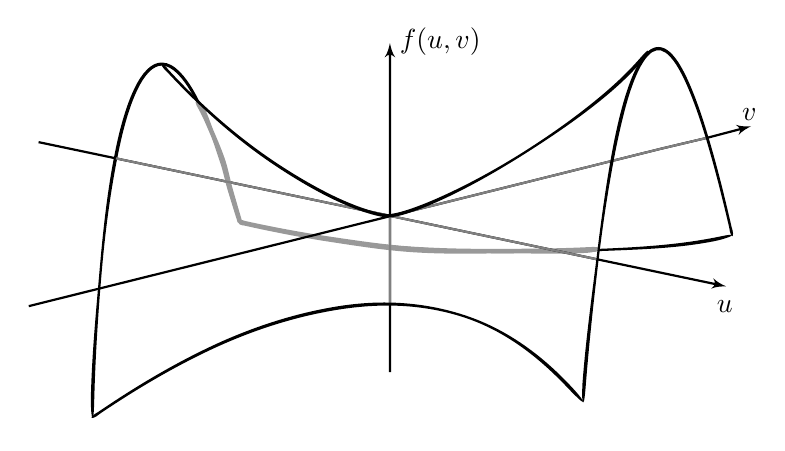
\begin{tikzpicture}[y=0.80pt, x=0.8pt,yscale=-1,scale=0.45, inner sep=0pt, outer sep=0pt]
\begin{scope}[shift={(-101.8437,-349.74693)}]% layer1
  % path2584
  \path[draw=black,line join=miter,line cap=butt,line width=0.800pt,latex'-]
    (464.4540,349.7469) -- (464.4542,523.5304) -- (464.4540,611.3544) --
    (464.4540,680.1289);

  % path2596
  \path[fill=black] (794.6845,544.1187) .. controls (775.3674,548.1155) and
    (755.7468,550.7347) .. (736.0117,552.5526) .. controls (716.2766,554.3705) and
    (696.4222,555.3886) .. (676.5759,556.1962) .. controls (675.7136,556.2313) and
    (674.8512,556.2654) .. (673.9889,556.2985) .. controls (635.1602,557.7871) and
    (596.2500,557.2700) .. (557.3357,557.0271) .. controls (547.3750,556.9649) and
    (537.4145,556.7954) .. (527.4552,556.5756) .. controls (497.6866,555.9192) and
    (468.0492,553.2278) .. (438.4991,549.8934) .. controls (399.0782,545.4452) and
    (359.9045,538.5570) .. (321.1686,529.9428) .. controls (315.9626,528.1162) and
    (313.2538,528.4191) .. (313.1617,529.3456) .. controls (313.0696,530.2722) and
    (315.6079,531.8241) .. (320.9202,532.3891) .. controls (359.3449,541.0949) and
    (398.2273,548.1139) .. (437.3881,552.7261) .. controls (467.2720,556.2457) and
    (497.2647,559.1183) .. (527.4085,559.8734) .. controls (536.7436,560.1071) and
    (546.0808,560.2922) .. (555.4192,560.3806) .. controls (574.5905,560.5621) and
    (594.6387,560.5028) .. (614.6994,560.1964) .. controls (634.7600,559.8899) and
    (654.8317,559.3298) .. (674.0591,558.5796) .. controls (675.1400,558.5375) and
    (676.2184,558.4949) .. (677.2941,558.4516) .. controls (696.9656,557.6616) and
    (715.7432,557.0134) .. (734.4549,555.6482) .. controls (753.1666,554.2829) and
    (771.8323,552.2213) .. (791.0966,548.3635) .. controls (794.6071,547.6205) and
    (799.9322,546.2087) .. (803.5598,544.8817) .. controls (807.1874,543.5547) and
    (809.1209,542.3626) .. (805.9498,542.1806) .. controls (802.5752,542.4615) and
    (798.4000,543.3933) .. (794.6845,544.1187) -- cycle;

  % path2600
  \path[draw=c999999,fill=c999999,line join=miter,line cap=butt,line
    width=0.800pt] (664.5285,555.6182) .. controls (635.6593,557.1110) and
    (606.6972,557.2203) .. (577.7098,557.4482) .. controls (562.8964,557.5646) and
    (548.0756,557.3726) .. (533.2538,557.0997) .. controls (519.0882,556.8391) and
    (504.9358,556.2076) .. (490.7919,555.4021) .. controls (476.3289,554.5784) and
    (461.9089,553.0740) .. (447.5384,551.2510) .. controls (433.1678,549.4279) and
    (418.8460,547.2867) .. (404.5179,545.1834) .. controls (375.8620,540.9770) and
    (347.3644,535.6356) .. (319.0831,529.4467) .. controls (315.3238,527.9558) and
    (313.2867,528.4271) .. (313.1604,529.3454) .. controls (313.0342,530.2636) and
    (314.8290,531.6304) .. (318.7460,531.8724) .. controls (346.7902,538.1746) and
    (375.0630,543.6544) .. (403.5114,548.0083) .. controls (417.7356,550.1852) and
    (431.9575,552.4024) .. (446.2319,554.3016) .. controls (460.5063,556.2007) and
    (474.8339,557.7816) .. (489.2084,558.6802) .. controls (503.4183,559.5686) and
    (518.3148,559.9855) .. (533.2133,559.9683) .. controls (548.4311,559.9499) and
    (563.6516,559.8281) .. (578.1719,559.7270) .. controls (592.5279,559.6269) and
    (606.2002,559.8776) .. (619.8647,559.9701) .. controls (633.5292,560.0626) and
    (647.1870,559.9981) .. (661.4839,559.2297) .. controls (666.7026,558.8705) and
    (677.4359,557.2338) .. (672.9021,555.6924) .. controls (670.4316,555.3384) and
    (667.3002,555.5174) .. (664.5285,555.6182) -- cycle;

  % path2586
  \path[draw=black,line join=miter,line cap=butt,line width=0.800pt,-latex']
    (111.8299,449.1826) -- (189.4412,465.4631) -- (284.3774,485.3780) --
    (456.9250,521.5734) -- (629.4725,557.7688) -- (672.6094,566.8177) --
    (715.7463,575.8665) -- (802.0201,593.9642);

  % path2582
  \path[draw=black,line join=miter,line cap=butt,line width=0.800pt,-latex']
    (101.9645,613.7853) -- (464.4542,523.5304) -- (645.6990,478.4030) --
    (736.3214,455.8392) -- (783.1148,444.7716) -- (826.9438,433.2755);

  % path2711
  \path[draw=c808080,line join=miter,line cap=butt,line width=0.800pt]
    (464.4542,523.5304) -- (464.4540,611.3544);

  % path2576
  \path[fill=black] (649.7173,698.0632) .. controls (638.3462,685.5487) and
    (626.1168,673.8120) .. (612.8932,663.2669) .. controls (597.2991,650.8322) and
    (580.3066,640.0958) .. (562.1612,631.7772) .. controls (562.1612,631.7772) and
    (562.1612,631.7772) .. (562.1612,631.7772) .. controls (555.5662,628.7557) and
    (548.8289,626.0765) .. (541.9793,623.7369) .. controls (526.7692,618.5416) and
    (511.0586,614.8550) .. (495.1145,612.6401) .. controls (479.1704,610.4252) and
    (462.9935,609.6840) .. (446.9098,610.3957) .. controls (434.9962,610.9237) and
    (423.1470,612.1765) .. (411.4020,614.0822) .. controls (394.7005,616.7920) and
    (378.1560,620.5310) .. (361.8337,625.1701) .. controls (345.5113,629.8093) and
    (329.4147,635.3496) .. (313.6853,641.6451) .. controls (304.2280,645.4285) and
    (294.8881,649.4838) .. (285.6815,653.8136) .. controls (245.8500,672.5461) and
    (207.9744,695.2362) .. (171.7092,719.9607) .. controls (166.3333,722.8356) and
    (164.5149,725.2166) .. (165.1490,725.9011) .. controls (165.7832,726.5856) and
    (168.8599,725.5841) .. (173.3532,721.7961) .. controls (209.3149,697.4964) and
    (246.8150,675.2249) .. (286.1521,656.8405) .. controls (295.5842,652.4324) and
    (305.1531,648.3155) .. (314.8404,644.4859) .. controls (330.1977,638.4168) and
    (345.8834,633.0675) .. (361.7609,628.5688) .. controls (377.6383,624.0700) and
    (393.7042,620.4212) .. (409.8949,617.7367) .. controls (421.9400,615.7396) and
    (434.3885,614.2801) .. (447.0571,613.6010) .. controls (463.1119,612.7383) and
    (479.5126,613.2627) .. (495.5527,615.3415) .. controls (511.5929,617.4203) and
    (527.2628,621.0573) .. (541.8956,626.1173) .. controls (548.5358,628.4135) and
    (554.9525,631.0284) .. (561.1571,633.9393) .. controls (570.2500,638.2031) and
    (578.8796,643.0574) .. (587.1378,648.3864) .. controls (595.3960,653.7154) and
    (603.2839,659.5201) .. (610.8904,665.7483) .. controls (622.3925,675.1656) and
    (633.2641,685.5332) .. (643.9146,696.8643) .. controls (646.6412,699.7077) and
    (650.8876,704.0120) .. (654.0172,706.8921) .. controls (655.5820,708.3321) and
    (656.8768,709.4069) .. (657.5985,709.7220) .. controls (658.3202,710.0371) and
    (658.4732,709.5895) .. (657.7192,708.0009) .. controls (655.6851,704.8277) and
    (652.5308,701.2229) .. (649.7173,698.0632) -- cycle;

  % path2709
  \path[draw=c808080,line join=miter,line cap=butt,line width=0.800pt]
    (464.4542,523.5304) -- (645.6990,478.4030) -- (736.3214,455.8392) --
    (783.1148,444.7716);

  % path2592
  \path[fill=black] (167.5760,711.1835) .. controls (168.6399,667.3314) and
    (171.3826,623.4775) .. (175.1461,579.6755) .. controls (175.1700,579.3972) and
    (175.1940,579.1190) .. (175.2180,578.8407) .. controls (178.4257,541.6197) and
    (183.1528,504.4939) .. (190.2472,467.8213) .. controls (191.5553,461.0602) and
    (192.9457,454.3157) .. (194.4639,447.6039) .. controls (196.0585,440.5539) and
    (197.8462,433.5518) .. (199.8726,426.6209) .. controls (202.8992,416.2761) and
    (206.3998,406.0693) .. (211.0640,396.4439) .. controls (211.0640,396.4439) and
    (211.0640,396.4439) .. (211.0640,396.4439) .. controls (214.3394,389.7192) and
    (218.0530,383.1770) .. (223.2633,378.1774) .. controls (225.1492,376.3681) and
    (227.2098,374.7875) .. (229.4719,373.7456) .. controls (229.4719,373.7456) and
    (229.4719,373.7456) .. (229.4719,373.7456) .. controls (231.4274,372.8403) and
    (233.5535,372.3238) .. (235.6439,372.3506) .. controls (238.2746,372.3556) and
    (240.9289,373.2087) .. (243.3660,374.4955) .. controls (243.3660,374.4955) and
    (243.3660,374.4955) .. (243.3660,374.4955) .. controls (246.4812,376.1464) and
    (249.2462,378.5355) .. (251.8105,381.1739) .. controls (256.3763,385.8829) and
    (260.2022,391.2751) .. (263.6569,396.9826) .. controls (266.0796,400.9850) and
    (268.3064,405.1497) .. (270.4562,409.3453) .. controls (288.3443,444.3684) and
    (299.6681,482.4538) .. (310.2415,520.5362) .. controls (311.2469,526.6000) and
    (312.8801,529.1233) .. (313.7355,528.7499) .. controls (314.5909,528.3765) and
    (314.6692,525.1019) .. (312.5088,519.5657) .. controls (302.1049,481.5221) and
    (290.8846,443.3554) .. (273.0395,408.0464) .. controls (271.0283,404.0595) and
    (268.9255,400.0775) .. (266.6314,396.2085) .. controls (263.0037,390.0904) and
    (258.9278,384.2389) .. (253.9814,379.0663) .. controls (251.3048,376.2638) and
    (248.2949,373.6721) .. (244.7965,371.7786) .. controls (244.7965,371.7786) and
    (244.7965,371.7786) .. (244.7965,371.7786) .. controls (242.0275,370.2771) and
    (238.8978,369.2938) .. (235.6439,369.2457) .. controls (233.0377,369.2229) and
    (230.4607,369.8319) .. (228.1212,370.9202) .. controls (225.4541,372.1650) and
    (223.1024,373.9372) .. (221.0431,375.9266) .. controls (215.4144,381.3632) and
    (211.4599,388.1995) .. (208.1357,395.0630) .. controls (208.1357,395.0630) and
    (208.1357,395.0630) .. (208.1357,395.0630) .. controls (203.3372,404.9102) and
    (199.7452,415.2732) .. (196.6755,425.7007) .. controls (196.6755,425.7007) and
    (196.6755,425.7007) .. (196.6755,425.7007) .. controls (194.8131,432.0202) and
    (193.1500,438.3918) .. (191.6530,444.7976) .. controls (189.9404,452.1258) and
    (188.4002,459.6116) .. (186.9800,467.1892) .. controls (183.5290,485.6002) and
    (180.7612,504.5838) .. (178.4941,523.4916) .. controls (176.2270,542.3994) and
    (174.4506,561.2306) .. (172.8840,579.3435) .. controls (172.8810,579.3834) and
    (172.8770,579.4233) .. (172.8736,579.4632) .. controls (172.8736,579.4632) and
    (172.8736,579.4632) .. (172.8736,579.4632) .. controls (170.9856,601.2809) and
    (169.1127,622.0538) .. (167.5545,642.8400) .. controls (165.9962,663.6262) and
    (164.7574,684.4242) .. (164.2456,706.2509) .. controls (164.1370,714.2318) and
    (164.8371,730.7255) .. (166.7677,723.9425) .. controls (167.3351,720.2057) and
    (167.4307,715.4169) .. (167.5760,711.1835) -- cycle;

  % path2604
  \path[draw=c999999,fill=c999999,line join=miter,line cap=butt,line
    width=0.800pt] (271.6535,412.4259) .. controls (276.7388,421.1544) and
    (280.6497,430.4900) .. (284.6566,439.7976) .. controls (288.6635,449.1051) and
    (291.5582,458.8592) .. (294.8557,468.4808) .. controls (298.1533,478.1024) and
    (299.9464,488.1968) .. (302.9376,497.9326) .. controls (305.9287,507.6682) and
    (308.8734,517.4268) .. (311.9747,527.1183) .. controls (311.5691,530.1299) and
    (316.3008,528.7010) .. (314.3123,526.4203) .. controls (311.4006,516.7691) and
    (308.6477,507.0402) .. (305.8328,497.3235) .. controls (303.0180,487.6068) and
    (301.3856,477.5212) .. (298.2167,467.9012) .. controls (295.0480,458.2811) and
    (290.6766,448.0864) .. (286.7133,438.8143) .. controls (284.7316,434.1782) and
    (283.1619,429.6385) .. (281.4472,425.1489) .. controls (279.7324,420.6592) and
    (277.8723,416.2178) .. (275.3072,411.8657) .. controls (274.2998,410.3108) and
    (271.4340,407.5206) .. (270.6361,409.6719) .. controls (270.6378,410.6311) and
    (271.2036,411.5695) .. (271.6535,412.4259) -- cycle;

  % path2707
  \path[draw=c808080,line join=miter,line cap=butt,line width=0.800pt]
    (189.4412,465.4631) -- (284.3774,485.3780) -- (456.9250,521.5734) --
    (629.4725,557.7688) -- (672.6094,566.8177);

  % path2578
  \path[fill=black] (660.8454,695.6273) .. controls (663.6771,659.4536) and
    (667.3746,623.3158) .. (671.5604,587.2077) .. controls (672.6923,577.4435) and
    (673.8566,567.6807) .. (675.0576,557.9209) .. controls (677.9779,534.1893) and
    (681.4609,510.5214) .. (685.5405,486.9536) .. controls (689.3445,464.9828) and
    (693.5652,443.0766) .. (699.0215,421.4935) .. controls (699.7407,418.6488) and
    (700.4892,415.8115) .. (701.2685,412.9825) .. controls (703.7063,404.1347) and
    (706.4492,395.3769) .. (709.8146,386.8782) .. controls (709.8146,386.8782) and
    (709.8146,386.8782) .. (709.8146,386.8782) .. controls (712.3328,380.5275) and
    (715.1431,374.3062) .. (718.7879,368.6509) .. controls (720.1658,366.5135) and
    (721.6537,364.4724) .. (723.3360,362.6433) .. controls (724.7094,361.1549) and
    (726.1879,359.8051) .. (727.8242,358.7746) .. controls (729.1912,357.9164) and
    (730.6580,357.2636) .. (732.1559,356.9919) .. controls (733.5626,356.7250) and
    (735.0423,356.7840) .. (736.4428,357.1330) .. controls (738.0316,357.5196) and
    (739.5613,358.2980) .. (741.0012,359.2629) .. controls (742.7843,360.4638) and
    (744.3954,361.9777) .. (745.9088,363.6261) .. controls (745.9088,363.6261) and
    (745.9088,363.6261) .. (745.9088,363.6261) .. controls (750.1538,368.2525) and
    (753.4362,373.7820) .. (756.4757,379.4810) .. controls (760.3269,386.7296) and
    (763.6130,394.2935) .. (766.6793,401.9731) .. controls (767.0916,403.0058) and
    (767.4993,404.0408) .. (767.9030,405.0777) .. controls (767.9030,405.0777) and
    (767.9030,405.0777) .. (767.9030,405.0777) .. controls (772.4573,416.7804) and
    (776.4377,428.7199) .. (780.1568,440.7494) .. controls (789.7361,471.7353) and
    (797.6244,503.2349) .. (804.9989,534.8322) .. controls (805.8121,541.1891) and
    (807.3638,543.9020) .. (808.2326,543.5584) .. controls (809.1015,543.2148) and
    (809.2854,539.8086) .. (807.2985,533.9409) .. controls (800.0555,502.4101) and
    (792.2923,470.9428) .. (782.8339,439.9415) .. controls (779.1473,427.8576) and
    (775.1879,415.8389) .. (770.6414,404.0292) .. controls (770.6414,404.0292) and
    (770.6414,404.0292) .. (770.6414,404.0292) .. controls (770.3461,403.2619) and
    (770.0485,402.4952) .. (769.7482,401.7293) .. controls (766.5956,393.6890) and
    (763.1936,385.7215) .. (759.1554,378.0455) .. controls (756.1032,372.2312) and
    (752.6903,366.4764) .. (748.1888,361.5076) .. controls (746.5752,359.7258) and
    (744.7827,358.0468) .. (742.7352,356.6486) .. controls (741.0762,355.5119) and
    (739.2129,354.5812) .. (737.1739,354.0620) .. controls (735.3447,353.6034) and
    (733.4144,353.5300) .. (731.5349,353.8794) .. controls (729.5605,354.2578) and
    (727.7205,355.0558) .. (726.0854,356.0984) .. controls (724.1436,357.3334) and
    (722.4478,358.8598) .. (720.9470,360.4963) .. controls (719.1021,362.5016) and
    (717.4972,364.6841) .. (716.0492,366.9270) .. controls (712.2277,372.8447) and
    (709.3051,379.2457) .. (706.7433,385.6879) .. controls (706.7433,385.6879) and
    (706.7433,385.6879) .. (706.7433,385.6879) .. controls (703.3018,394.3241) and
    (700.5039,403.1822) .. (698.0344,412.0902) .. controls (698.0344,412.0902) and
    (698.0344,412.0902) .. (698.0344,412.0902) .. controls (697.4403,414.2326) and
    (696.8641,416.3792) .. (696.3050,418.5297) .. controls (693.4805,429.3945) and
    (690.9961,440.5981) .. (688.7653,451.9768) .. controls (686.5346,463.3555) and
    (684.5557,474.9089) .. (682.7013,486.4701) .. controls (678.8074,510.7378) and
    (675.5733,535.1100) .. (672.7027,558.3703) .. controls (671.5072,568.0573) and
    (670.3144,577.5441) .. (669.1318,586.9157) .. controls (664.7686,621.4932) and
    (660.5564,654.5306) .. (657.8004,690.3155) .. controls (657.2390,698.6276) and
    (656.9735,715.8563) .. (659.2989,708.8871) .. controls (660.0845,705.0215) and
    (660.4578,700.0336) .. (660.8454,695.6273) -- cycle;

  % path2580
  \path[fill=black] (712.6004,368.1947) .. controls (697.8632,384.6697) and
    (681.0130,399.3670) .. (663.5613,413.2056) .. controls (644.1762,428.5714) and
    (623.8539,442.7722) .. (602.9907,456.1641) .. controls (598.3205,459.1618) and
    (593.6134,462.1038) .. (588.8745,464.9942) .. controls (565.5125,479.2421) and
    (541.3973,492.2981) .. (516.4679,503.5573) .. controls (506.7540,507.9441) and
    (496.9249,512.0596) .. (486.8820,515.5425) .. controls (483.5392,516.6996) and
    (480.1823,517.8127) .. (476.8006,518.7790) .. controls (472.8399,519.9107) and
    (468.8404,520.8261) .. (464.7898,521.3595) .. controls (463.6477,521.5180) and
    (462.4232,521.4415) .. (461.1505,521.3353) .. controls (459.2416,521.1673) and
    (457.3307,520.8498) .. (455.4162,520.4721) .. controls (449.6841,519.3397) and
    (444.0505,517.6614) .. (438.4744,515.7772) .. controls (420.4271,509.6759) and
    (403.2075,501.3020) .. (386.5373,492.0202) .. controls (373.7411,484.8948) and
    (361.2962,477.2040) .. (349.1323,469.0828) .. controls (310.0827,443.0118) and
    (274.6394,411.4227) .. (242.5348,376.9676) .. controls (238.5784,371.7634) and
    (235.8749,370.1064) .. (235.2875,370.8337) .. controls (234.7001,371.5610) and
    (236.2492,374.6904) .. (240.9889,378.8923) .. controls (272.7985,413.2486) and
    (307.9469,444.8209) .. (346.7309,471.0101) .. controls (359.1762,479.4138) and
    (371.9222,487.3748) .. (385.0458,494.7464) .. controls (401.7923,504.1537) and
    (419.1631,512.6612) .. (437.4450,518.8983) .. controls (437.4450,518.8983) and
    (437.4450,518.8983) .. (437.4450,518.8983) .. controls (443.0891,520.8252) and
    (448.8539,522.5523) .. (454.7824,523.7399) .. controls (456.7618,524.1372) and
    (458.7878,524.4749) .. (460.8627,524.6639) .. controls (462.2028,524.7966) and
    (463.6703,524.8700) .. (465.2321,524.6788) .. controls (468.7231,524.2181) and
    (472.1503,523.5020) .. (475.5198,522.6224) .. controls (479.7239,521.5248) and
    (483.8751,520.1670) .. (487.9809,518.7286) .. controls (498.0181,515.2243) and
    (507.9499,510.9971) .. (517.7774,506.4411) .. controls (542.7449,494.8680) and
    (567.1790,481.0997) .. (590.0762,466.9796) .. controls (595.0784,463.8952) and
    (600.0094,460.7916) .. (604.8547,457.6796) .. controls (626.2580,443.9331) and
    (646.2312,430.3740) .. (665.4281,415.5828) .. controls (673.4713,409.3880) and
    (681.4121,402.9830) .. (689.1600,396.1733) .. controls (696.9079,389.3636) and
    (704.4655,382.1495) .. (711.6859,374.3220) .. controls (713.1174,372.7412) and
    (714.8720,370.6866) .. (716.5733,368.5417) .. controls (718.2746,366.3968) and
    (719.9215,364.1615) .. (721.1820,362.2551) .. controls (722.4426,360.3487) and
    (723.3193,358.7741) .. (723.5155,357.9664) .. controls (723.7117,357.1588) and
    (723.2340,357.1237) .. (721.7516,358.2468) .. controls (718.8781,361.0242) and
    (715.6172,364.8859) .. (712.6004,368.1947) -- cycle;

  % text3394
  \path[shift={(101.8437,349.74693)},fill=black] (690.8363,270.26215) node[above
    right] (text3394) {$u$};

  % text3398
  \path[shift={(101.8437,349.74693)},fill=black] (716.22119,77.487068) node[above
    right] (text3398) {$v$};

  % text3402
  \path[shift={(101.8437,349.74693)},fill=black] (372.68695,12.317032) node[above
    right] (text3402) {$f(u,v)$};

\end{scope}

\end{tikzpicture}


\end{center}

\end{itemize}

\end{przyklad}

\end{frame}
%%%%%%next-slide%%%%%
\mode<all>{\lowsection{Powierzchnie obrotowe}}
\begin{frame}[<+->]

\begin{definicja}
\textbf{Powierzchnia obrotowa} powstaje poprzez obrócenie krzywej $\alpha(t)$ 
wokół pewnej ustalonej prostej $l$. Postać ogólna to 
\[x(t,\phi)=\alpha(t)\cdot Rot_l(\phi),\] 
gdzie $Rot_l(\phi)$ to macierz $3\times 3$ obrotu o kąt $\phi$ wokoł prostej 
$l$.
\begin{center}

\definecolor{c808080}{RGB}{128,128,128}
\usetikzlibrary{arrows}
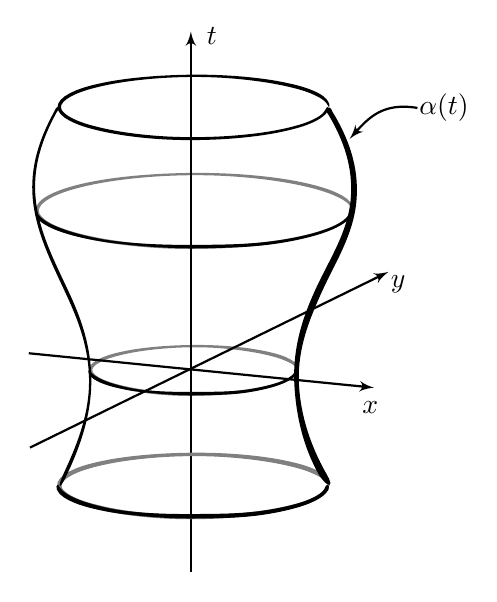
\begin{tikzpicture}[y=0.80pt, x=0.8pt,yscale=-1,scale=0.45, inner sep=0pt, outer sep=0pt]
\begin{scope}[shift={(-173.42489,-122.74609)}]% layer1
  \begin{scope}[shift={(2933.0824,1766.7171)}]% g3632
    % path3588
    \path[fill=c808080] (-2496.3141,-1307.2948) .. controls (-2496.7759,-1307.5577)
      and (-2497.2395,-1307.8062) .. (-2497.7018,-1308.0428) .. controls
      (-2497.7018,-1308.0428) and (-2497.7018,-1308.0428) .. (-2497.7018,-1308.0428)
      .. controls (-2504.9716,-1311.8175) and (-2512.8326,-1313.8464) ..
      (-2520.5587,-1315.5283) .. controls (-2520.5587,-1315.5283) and
      (-2520.5587,-1315.5283) .. (-2520.5587,-1315.5283) .. controls
      (-2531.5315,-1317.9373) and (-2542.6575,-1319.4283) .. (-2553.7913,-1320.4578)
      .. controls (-2567.2669,-1321.7053) and (-2580.8033,-1322.2289) ..
      (-2594.3280,-1322.1207) .. controls (-2596.5762,-1322.1027) and
      (-2598.8246,-1322.0677) .. (-2601.0726,-1322.0135) .. controls
      (-2612.3389,-1321.7433) and (-2623.6003,-1321.1394) .. (-2634.8253,-1320.0554)
      .. controls (-2634.8253,-1320.0554) and (-2634.8253,-1320.0554) ..
      (-2634.8253,-1320.0554) .. controls (-2645.9373,-1318.9832) and
      (-2657.0444,-1317.4741) .. (-2667.9716,-1314.9854) .. controls
      (-2667.9716,-1314.9854) and (-2667.9716,-1314.9854) .. (-2667.9716,-1314.9854)
      .. controls (-2675.6658,-1313.2426) and (-2683.4636,-1311.1341) ..
      (-2690.5352,-1307.2768) .. controls (-2690.5352,-1307.2768) and
      (-2690.5352,-1307.2768) .. (-2690.5352,-1307.2768) .. controls
      (-2692.8129,-1306.0448) and (-2695.0801,-1304.5503) .. (-2696.9079,-1302.4972)
      .. controls (-2698.2534,-1301.0209) and (-2699.2663,-1299.0546) ..
      (-2699.3073,-1296.8434) .. controls (-2699.2843,-1295.9609) and
      (-2699.1079,-1295.1198) .. (-2698.8174,-1294.3347) .. controls
      (-2698.3801,-1293.1529) and (-2697.6872,-1292.0973) .. (-2696.8776,-1291.2165)
      .. controls (-2695.0451,-1289.1774) and (-2692.7825,-1287.6919) ..
      (-2690.5092,-1286.4575) .. controls (-2683.4515,-1282.5939) and
      (-2675.6805,-1280.4014) .. (-2668.0072,-1278.5475) .. controls
      (-2668.0072,-1278.5475) and (-2668.0072,-1278.5475) .. (-2668.0072,-1278.5475)
      .. controls (-2657.1087,-1275.8993) and (-2646.0099,-1274.1694) ..
      (-2634.8915,-1272.9550) .. controls (-2622.2147,-1271.5687) and
      (-2609.4620,-1270.8929) .. (-2596.7226,-1270.9167) .. controls
      (-2595.9243,-1270.9167) and (-2595.1261,-1270.9267) .. (-2594.3280,-1270.9277)
      .. controls (-2580.7872,-1271.0227) and (-2567.2448,-1271.7081) ..
      (-2553.7840,-1273.1542) .. controls (-2542.6653,-1274.3475) and
      (-2531.5647,-1276.0287) .. (-2520.6807,-1278.6862) .. controls
      (-2520.6807,-1278.6862) and (-2520.6807,-1278.6862) .. (-2520.6807,-1278.6862)
      .. controls (-2513.0114,-1280.5493) and (-2505.2523,-1282.7814) ..
      (-2498.2863,-1286.7130) .. controls (-2498.2863,-1286.7130) and
      (-2498.2863,-1286.7130) .. (-2498.2863,-1286.7130) .. controls
      (-2496.5280,-1287.6994) and (-2494.7878,-1288.8332) .. (-2493.2773,-1290.2488)
      .. controls (-2492.7799,-1290.6081) and (-2492.3400,-1290.9876) ..
      (-2491.9568,-1291.3747) .. controls (-2491.2460,-1292.0809) and
      (-2490.7541,-1292.8561) .. (-2490.4649,-1293.5658) .. controls
      (-2490.1757,-1294.2754) and (-2490.0830,-1294.9181) .. (-2490.1054,-1295.4238)
      .. controls (-2490.1274,-1295.9296) and (-2490.2622,-1296.2995) ..
      (-2490.4323,-1296.5298) .. controls (-2490.6024,-1296.7601) and
      (-2490.8071,-1296.8530) .. (-2491.0069,-1296.8430) .. controls
      (-2491.4065,-1296.8230) and (-2491.7604,-1296.4255) .. (-2492.1918,-1295.8342)
      .. controls (-2492.6232,-1295.2430) and (-2493.1845,-1294.4202) ..
      (-2494.0402,-1293.2177) .. controls (-2494.3507,-1292.8046) and
      (-2494.7007,-1292.3594) .. (-2495.1022,-1291.8771) .. controls
      (-2496.3680,-1290.7417) and (-2497.8845,-1289.7818) .. (-2499.4707,-1288.8788)
      .. controls (-2499.4707,-1288.8788) and (-2499.4707,-1288.8788) ..
      (-2499.4707,-1288.8788) .. controls (-2506.1022,-1285.1453) and
      (-2513.6538,-1283.0335) .. (-2521.2624,-1281.2008) .. controls
      (-2521.2624,-1281.2008) and (-2521.2624,-1281.2008) .. (-2521.2624,-1281.2008)
      .. controls (-2532.0102,-1278.6269) and (-2543.0036,-1277.0182) ..
      (-2554.0509,-1275.8830) .. controls (-2567.4181,-1274.5105) and
      (-2580.8707,-1273.8937) .. (-2594.3280,-1273.8608) .. controls
      (-2594.8939,-1273.8608) and (-2595.4598,-1273.8608) .. (-2596.0257,-1273.8598)
      .. controls (-2608.9127,-1273.8758) and (-2621.7982,-1274.6114) ..
      (-2634.5866,-1276.0718) .. controls (-2634.5866,-1276.0718) and
      (-2634.5866,-1276.0718) .. (-2634.5866,-1276.0718) .. controls
      (-2645.6132,-1277.3320) and (-2656.5691,-1279.0871) .. (-2667.2701,-1281.7344)
      .. controls (-2667.2701,-1281.7344) and (-2667.2701,-1281.7344) ..
      (-2667.2701,-1281.7344) .. controls (-2674.8495,-1283.6243) and
      (-2682.3343,-1285.7354) .. (-2688.9043,-1289.3924) .. controls
      (-2688.9043,-1289.3924) and (-2688.9043,-1289.3924) .. (-2688.9043,-1289.3924)
      .. controls (-2691.0064,-1290.5807) and (-2692.9649,-1291.8317) ..
      (-2694.3587,-1293.4450) .. controls (-2694.6257,-1293.7729) and
      (-2694.8776,-1294.1078) .. (-2695.0986,-1294.4442) .. controls
      (-2695.6342,-1295.2594) and (-2695.9902,-1296.0864) .. (-2695.9327,-1296.8437)
      .. controls (-2696.0237,-1297.9047) and (-2695.2996,-1299.1247) ..
      (-2694.3829,-1300.2638) .. controls (-2694.3829,-1300.2638) and
      (-2694.3829,-1300.2638) .. (-2694.3829,-1300.2638) .. controls
      (-2693.0020,-1301.8821) and (-2691.0460,-1303.1489) .. (-2688.9339,-1304.3493)
      .. controls (-2682.4328,-1307.9891) and (-2674.9232,-1310.1150) ..
      (-2667.2791,-1311.9922) .. controls (-2656.5780,-1314.5996) and
      (-2645.5540,-1316.2966) .. (-2634.5768,-1317.5162) .. controls
      (-2623.0657,-1318.7939) and (-2611.6070,-1319.5005) .. (-2600.4714,-1319.7448)
      .. controls (-2598.4129,-1319.7898) and (-2596.3654,-1319.8148) ..
      (-2594.3280,-1319.8218) .. controls (-2594.3280,-1319.8218) and
      (-2594.3280,-1319.8218) .. (-2594.3280,-1319.8218) .. controls
      (-2580.5442,-1319.8658) and (-2567.2326,-1319.0787) .. (-2554.0702,-1317.6078)
      .. controls (-2543.0855,-1316.3792) and (-2532.2031,-1314.7239) ..
      (-2521.3235,-1312.2230) .. controls (-2514.5547,-1310.6555) and
      (-2507.7494,-1308.9499) .. (-2501.3880,-1306.0134) .. controls
      (-2500.7626,-1305.7343) and (-2500.0646,-1305.4190) .. (-2499.3269,-1305.0720)
      .. controls (-2498.2704,-1304.5701) and (-2497.1366,-1304.0156) ..
      (-2496.0582,-1303.3913) .. controls (-2494.9797,-1302.7669) and
      (-2493.9611,-1302.0672) .. (-2493.0833,-1301.3165) .. controls
      (-2492.3068,-1300.6462) and (-2491.6423,-1299.9192) .. (-2491.1545,-1299.2378)
      .. controls (-2490.6668,-1298.5563) and (-2490.3492,-1297.9187) ..
      (-2490.0986,-1297.4678) .. controls (-2489.8480,-1297.0168) and
      (-2489.6440,-1296.7543) .. (-2489.4244,-1296.8718) .. controls
      (-2489.2047,-1296.9894) and (-2488.9540,-1297.5038) .. (-2488.9465,-1298.5326)
      .. controls (-2489.1326,-1300.1397) and (-2489.9172,-1301.8123) ..
      (-2491.0665,-1303.1005) .. controls (-2492.5772,-1304.8614) and
      (-2494.5060,-1306.2369) .. (-2496.3141,-1307.2948) -- cycle;

    % path3592
    \path[fill=black] (-2697.3247,-1290.2935) .. controls (-2695.3568,-1288.3459)
      and (-2693.0878,-1286.9626) .. (-2690.8473,-1285.8393) .. controls
      (-2683.5759,-1282.1451) and (-2675.7554,-1280.1118) .. (-2668.0366,-1278.4205)
      .. controls (-2668.0366,-1278.4205) and (-2668.0366,-1278.4205) ..
      (-2668.0366,-1278.4205) .. controls (-2660.8171,-1276.8274) and
      (-2653.5239,-1275.6404) .. (-2646.1951,-1274.8126) .. controls
      (-2642.4060,-1274.3846) and (-2638.6155,-1273.9927) .. (-2634.8252,-1273.6321)
      .. controls (-2621.3678,-1272.3506) and (-2607.8494,-1271.5115) ..
      (-2594.3280,-1271.6259) .. controls (-2594.3280,-1271.6259) and
      (-2594.3280,-1271.6259) .. (-2594.3280,-1271.6259) .. controls
      (-2593.9680,-1271.6259) and (-2593.6081,-1271.6359) .. (-2593.2481,-1271.6369)
      .. controls (-2580.0904,-1271.7978) and (-2566.9023,-1271.7766) ..
      (-2553.7539,-1272.8461) .. controls (-2549.2262,-1273.2136) and
      (-2544.7000,-1273.7055) .. (-2540.2008,-1274.3990) .. controls
      (-2533.6141,-1275.4141) and (-2527.0620,-1276.6798) .. (-2520.5920,-1278.3021)
      .. controls (-2520.5920,-1278.3021) and (-2520.5920,-1278.3021) ..
      (-2520.5920,-1278.3021) .. controls (-2512.9220,-1280.2129) and
      (-2505.1444,-1282.5269) .. (-2498.1989,-1286.5529) .. controls
      (-2498.1989,-1286.5529) and (-2498.1989,-1286.5529) .. (-2498.1989,-1286.5529)
      .. controls (-2495.9609,-1287.8409) and (-2493.7509,-1289.3806) ..
      (-2492.0226,-1291.4324) .. controls (-2492.0226,-1291.4324) and
      (-2492.0226,-1291.4324) .. (-2492.0226,-1291.4324) .. controls
      (-2491.5831,-1291.9449) and (-2491.1844,-1292.5096) .. (-2490.8526,-1293.1142)
      .. controls (-2490.3889,-1293.6179) and (-2490.1039,-1294.1593) ..
      (-2489.9639,-1294.6498) .. controls (-2489.8240,-1295.1403) and
      (-2489.8264,-1295.5787) .. (-2489.9139,-1295.9195) .. controls
      (-2490.0891,-1296.6010) and (-2490.5831,-1296.8672) .. (-2491.0438,-1296.8413)
      .. controls (-2491.5045,-1296.8153) and (-2491.9351,-1296.5537) ..
      (-2492.2584,-1296.1672) .. controls (-2492.5816,-1295.7808) and
      (-2492.8006,-1295.2596) .. (-2493.0247,-1294.2650) .. controls
      (-2493.2674,-1293.8549) and (-2493.5540,-1293.4505) .. (-2493.8637,-1293.0611)
      .. controls (-2493.8637,-1293.0611) and (-2493.8637,-1293.0611) ..
      (-2493.8637,-1293.0611) .. controls (-2495.2923,-1291.3390) and
      (-2497.2905,-1290.0004) .. (-2499.4129,-1288.7727) .. controls
      (-2499.4129,-1288.7727) and (-2499.4129,-1288.7727) .. (-2499.4129,-1288.7727)
      .. controls (-2506.0331,-1284.9823) and (-2513.6003,-1282.8322) ..
      (-2521.2132,-1280.9880) .. controls (-2521.2132,-1280.9880) and
      (-2521.2132,-1280.9880) .. (-2521.2132,-1280.9880) .. controls
      (-2527.4936,-1279.4740) and (-2533.8606,-1278.3004) .. (-2540.2719,-1277.3642)
      .. controls (-2544.8406,-1276.6970) and (-2549.4434,-1276.2411) ..
      (-2554.0536,-1275.9110) .. controls (-2566.8296,-1274.9976) and
      (-2579.6398,-1275.1094) .. (-2592.4246,-1275.0134) .. controls
      (-2593.0569,-1275.0134) and (-2593.6914,-1275.0034) .. (-2594.3279,-1275.0004)
      .. controls (-2607.3667,-1274.9204) and (-2621.2538,-1275.0594) ..
      (-2634.5902,-1276.0330) .. controls (-2638.5157,-1276.3201) and
      (-2642.3925,-1276.6707) .. (-2646.1779,-1277.1077) .. controls
      (-2653.5664,-1277.9606) and (-2660.5695,-1279.3707) .. (-2667.4044,-1281.1531)
      .. controls (-2671.1647,-1282.1386) and (-2674.8929,-1283.1879) ..
      (-2678.5360,-1284.4258) .. controls (-2682.1792,-1285.6637) and
      (-2685.7356,-1287.0857) .. (-2689.1859,-1288.8769) .. controls
      (-2689.1859,-1288.8769) and (-2689.1859,-1288.8769) .. (-2689.1859,-1288.8769)
      .. controls (-2690.6945,-1289.6692) and (-2692.1693,-1290.4986) ..
      (-2693.4830,-1291.4958) .. controls (-2693.9676,-1291.8436) and
      (-2694.5541,-1292.2652) .. (-2695.1478,-1292.7465) .. controls
      (-2695.7108,-1293.2117) and (-2696.2927,-1293.7356) .. (-2696.7929,-1294.2738)
      .. controls (-2697.2931,-1294.8120) and (-2697.7068,-1295.3681) ..
      (-2698.0481,-1295.8418) .. controls (-2698.3895,-1296.3156) and
      (-2698.6710,-1296.7092) .. (-2698.9726,-1296.8159) .. controls
      (-2699.2742,-1296.9225) and (-2699.6209,-1296.7289) .. (-2699.8578,-1295.9836)
      .. controls (-2699.9368,-1295.0533) and (-2699.7278,-1294.0094) ..
      (-2699.3068,-1293.0624) .. controls (-2698.8858,-1292.1154) and
      (-2698.2597,-1291.2666) .. (-2697.5968,-1290.5801) .. controls
      (-2697.5062,-1290.4827) and (-2697.4153,-1290.3871) .. (-2697.3247,-1290.2935)
      -- cycle;

    % path3602
    \path[fill=c808080] (-2444.8213,-1471.9281) .. controls (-2445.5077,-1472.3250)
      and (-2446.1988,-1472.7024) .. (-2446.8897,-1473.0640) .. controls
      (-2451.7152,-1475.6193) and (-2456.7745,-1477.5693) .. (-2461.8565,-1479.2482)
      .. controls (-2461.8565,-1479.2482) and (-2461.8565,-1479.2482) ..
      (-2461.8565,-1479.2482) .. controls (-2468.2855,-1481.3762) and
      (-2474.8252,-1483.0774) .. (-2481.3926,-1484.5454) .. controls
      (-2481.3926,-1484.5454) and (-2481.3926,-1484.5454) .. (-2481.3926,-1484.5454)
      .. controls (-2498.0444,-1488.2680) and (-2514.9588,-1490.5713) ..
      (-2531.8985,-1492.1688) .. controls (-2552.3988,-1494.1037) and
      (-2572.9989,-1494.9278) .. (-2593.5875,-1494.8196) .. controls
      (-2597.0100,-1494.8016) and (-2600.4328,-1494.7576) .. (-2603.8552,-1494.6871)
      .. controls (-2621.0067,-1494.3317) and (-2638.1520,-1493.4238) ..
      (-2655.2372,-1491.7664) .. controls (-2655.2372,-1491.7664) and
      (-2655.2373,-1491.7664) .. (-2655.2373,-1491.7664) .. controls
      (-2672.1518,-1490.1264) and (-2689.0475,-1487.8055) .. (-2705.6569,-1484.0024)
      .. controls (-2705.6569,-1484.0024) and (-2705.6569,-1484.0024) ..
      (-2705.6569,-1484.0024) .. controls (-2712.2021,-1482.5038) and
      (-2718.7116,-1480.7647) .. (-2725.0927,-1478.5886) .. controls
      (-2725.0927,-1478.5886) and (-2725.0927,-1478.5886) .. (-2725.0927,-1478.5886)
      .. controls (-2730.1364,-1476.8708) and (-2735.1371,-1474.8830) ..
      (-2739.8664,-1472.2981) .. controls (-2739.8664,-1472.2981) and
      (-2739.8664,-1472.2981) .. (-2739.8664,-1472.2981) .. controls
      (-2743.3045,-1470.4315) and (-2746.7014,-1468.2026) .. (-2749.4056,-1465.1588)
      .. controls (-2750.4346,-1463.9996) and (-2751.3464,-1462.6834) ..
      (-2751.9991,-1461.2029) .. controls (-2752.5771,-1459.8874) and
      (-2752.9078,-1458.4455) .. (-2752.9090,-1456.9716) .. controls
      (-2752.8990,-1455.7169) and (-2752.6561,-1454.4877) .. (-2752.2231,-1453.3415)
      .. controls (-2752.1471,-1453.1413) and (-2752.0662,-1452.9437) ..
      (-2751.9795,-1452.7489) .. controls (-2751.3210,-1451.2741) and
      (-2750.4058,-1449.9649) .. (-2749.3753,-1448.8112) .. controls
      (-2746.6665,-1445.7814) and (-2743.2742,-1443.5616) .. (-2739.8405,-1441.6925)
      .. controls (-2735.1177,-1439.1052) and (-2730.1271,-1437.1002) ..
      (-2725.0931,-1435.3536) .. controls (-2718.7245,-1433.1415) and
      (-2712.2273,-1431.3483) .. (-2705.6925,-1429.7868) .. controls
      (-2689.1124,-1425.8243) and (-2672.2251,-1423.2825) .. (-2655.3035,-1421.5002)
      .. controls (-2655.3034,-1421.5002) and (-2655.3034,-1421.5002) ..
      (-2655.3034,-1421.5002) .. controls (-2636.0124,-1419.4668) and
      (-2616.6145,-1418.4870) .. (-2597.2311,-1418.4772) .. controls
      (-2596.0165,-1418.4766) and (-2594.8019,-1418.4772) .. (-2593.5875,-1418.4872)
      .. controls (-2572.9838,-1418.5822) and (-2552.3777,-1419.5680) ..
      (-2531.8911,-1421.7016) .. controls (-2514.9672,-1423.4629) and
      (-2498.0781,-1425.9562) .. (-2481.5146,-1429.9276) .. controls
      (-2481.5146,-1429.9276) and (-2481.5146,-1429.9276) .. (-2481.5146,-1429.9276)
      .. controls (-2474.9833,-1431.4934) and (-2468.4938,-1433.2995) ..
      (-2462.1437,-1435.5363) .. controls (-2462.1437,-1435.5363) and
      (-2462.1437,-1435.5363) .. (-2462.1437,-1435.5363) .. controls
      (-2457.1226,-1437.3034) and (-2452.1539,-1439.3348) .. (-2447.4741,-1441.9502)
      .. controls (-2444.8062,-1443.4340) and (-2442.1753,-1445.1266) ..
      (-2439.9003,-1447.2376) .. controls (-2439.1777,-1447.8017) and
      (-2438.5381,-1448.3848) .. (-2437.9783,-1448.9715) .. controls
      (-2436.7207,-1450.2910) and (-2435.9112,-1451.6741) .. (-2435.4869,-1452.8792)
      .. controls (-2435.0153,-1454.2209) and (-2435.0267,-1455.3123) ..
      (-2435.1843,-1455.9984) .. controls (-2435.3418,-1456.6845) and
      (-2435.6350,-1456.9840) .. (-2435.9087,-1456.9737) .. controls
      (-2436.1824,-1456.9637) and (-2436.4422,-1456.6537) .. (-2436.7392,-1456.1284)
      .. controls (-2437.0361,-1455.6030) and (-2437.3799,-1454.8565) ..
      (-2437.9019,-1453.9394) .. controls (-2438.3956,-1453.0651) and
      (-2439.0884,-1452.0316) .. (-2440.0617,-1450.8145) .. controls
      (-2440.5778,-1450.1688) and (-2441.1643,-1449.4867) .. (-2441.8353,-1448.7674)
      .. controls (-2443.8405,-1446.9820) and (-2446.2061,-1445.4928) ..
      (-2448.6586,-1444.1159) .. controls (-2453.1672,-1441.6067) and
      (-2458.0119,-1439.6482) .. (-2462.9594,-1437.9185) .. controls
      (-2462.9594,-1437.9185) and (-2462.9594,-1437.9185) .. (-2462.9594,-1437.9185)
      .. controls (-2469.2093,-1435.7366) and (-2475.6201,-1433.9749) ..
      (-2482.0963,-1432.4421) .. controls (-2482.0963,-1432.4421) and
      (-2482.0963,-1432.4421) .. (-2482.0963,-1432.4421) .. controls
      (-2498.5237,-1428.5545) and (-2515.3056,-1426.1336) .. (-2532.1581,-1424.4303)
      .. controls (-2552.5511,-1422.3704) and (-2573.0675,-1421.4532) ..
      (-2593.5875,-1421.4203) .. controls (-2594.4504,-1421.4203) and
      (-2595.3133,-1421.4203) .. (-2596.1762,-1421.4209) .. controls
      (-2615.8268,-1421.4619) and (-2635.4775,-1422.5000) .. (-2654.9985,-1424.6192)
      .. controls (-2671.8286,-1426.4472) and (-2688.5731,-1429.0142) ..
      (-2704.9553,-1432.9758) .. controls (-2711.4108,-1434.5371) and
      (-2717.7960,-1436.3138) .. (-2724.0191,-1438.4924) .. controls
      (-2724.0191,-1438.4924) and (-2724.0191,-1438.4924) .. (-2724.0191,-1438.4924)
      .. controls (-2728.9458,-1440.2205) and (-2733.7598,-1442.1587) ..
      (-2738.2355,-1444.6295) .. controls (-2738.2355,-1444.6295) and
      (-2738.2355,-1444.6295) .. (-2738.2355,-1444.6295) .. controls
      (-2741.4980,-1446.4526) and (-2744.5862,-1448.4379) .. (-2746.8563,-1451.0419)
      .. controls (-2747.3220,-1451.5752) and (-2747.7508,-1452.1224) ..
      (-2748.1196,-1452.6851) .. controls (-2748.4226,-1453.1473) and
      (-2748.6852,-1453.6206) .. (-2748.8943,-1454.1057) .. controls
      (-2748.8943,-1454.1057) and (-2748.8943,-1454.1057) .. (-2748.8943,-1454.1057)
      .. controls (-2749.2982,-1455.0358) and (-2749.5402,-1456.0228) ..
      (-2749.5344,-1456.9740) .. controls (-2749.5344,-1456.9740) and
      (-2749.5344,-1456.9740) .. (-2749.5344,-1456.9740) .. controls
      (-2749.5454,-1457.9213) and (-2749.3102,-1458.9107) .. (-2748.9084,-1459.8485)
      .. controls (-2748.4512,-1460.9242) and (-2747.7289,-1461.9483) ..
      (-2746.8805,-1462.9276) .. controls (-2746.8805,-1462.9276) and
      (-2746.8805,-1462.9276) .. (-2746.8805,-1462.9276) .. controls
      (-2744.6277,-1465.5315) and (-2741.5431,-1467.5346) .. (-2738.2651,-1469.3727)
      .. controls (-2733.8130,-1471.8400) and (-2728.9951,-1473.7872) ..
      (-2724.0418,-1475.5217) .. controls (-2724.0418,-1475.5217) and
      (-2724.0418,-1475.5217) .. (-2724.0418,-1475.5217) .. controls
      (-2717.8418,-1477.6886) and (-2711.4468,-1479.4593) .. (-2704.9644,-1481.0113)
      .. controls (-2688.5878,-1484.9316) and (-2671.7432,-1487.4445) ..
      (-2654.9888,-1489.2293) .. controls (-2637.4177,-1491.1000) and
      (-2619.9372,-1492.1029) .. (-2602.9557,-1492.4246) .. controls
      (-2599.8164,-1492.4846) and (-2596.6942,-1492.5156) .. (-2593.5875,-1492.5226)
      .. controls (-2572.5695,-1492.5666) and (-2552.2679,-1491.4695) ..
      (-2532.1774,-1489.3208) .. controls (-2515.4124,-1487.5266) and
      (-2498.7824,-1485.0719) .. (-2482.1573,-1481.2420) .. controls
      (-2475.7318,-1479.7615) and (-2469.3183,-1478.0744) .. (-2462.9800,-1475.9694)
      .. controls (-2459.1443,-1474.6936) and (-2455.3380,-1473.2864) ..
      (-2451.6567,-1471.5808) .. controls (-2450.6985,-1471.1464) and
      (-2449.6333,-1470.6497) .. (-2448.5147,-1470.0952) .. controls
      (-2446.9075,-1469.2921) and (-2445.1836,-1468.3880) .. (-2443.5538,-1467.3663)
      .. controls (-2441.9240,-1466.3447) and (-2440.3958,-1465.1979) ..
      (-2439.1047,-1463.9800) .. controls (-2437.9561,-1462.8975) and
      (-2437.0215,-1461.7590) .. (-2436.3597,-1460.6857) .. controls
      (-2435.3585,-1459.0623) and (-2435.0006,-1457.6177) .. (-2434.6716,-1457.1414)
      .. controls (-2434.5071,-1456.9032) and (-2434.3386,-1456.9041) ..
      (-2434.1780,-1457.2420) .. controls (-2434.0174,-1457.5799) and
      (-2433.8590,-1458.2629) .. (-2433.9187,-1459.3428) .. controls
      (-2434.0225,-1460.0599) and (-2434.2109,-1460.7908) .. (-2434.4852,-1461.5086)
      .. controls (-2435.0731,-1463.0402) and (-2435.9905,-1464.4956) ..
      (-2437.0879,-1465.7641) .. controls (-2439.2965,-1468.3119) and
      (-2442.1280,-1470.3420) .. (-2444.8213,-1471.9281) -- cycle;

    % path3604
    \path[fill=black] (-2749.7017,-1447.7551) .. controls (-2746.8759,-1444.8838)
      and (-2743.5271,-1442.8037) .. (-2740.1786,-1441.0744) .. controls
      (-2740.1785,-1441.0744) and (-2740.1785,-1441.0744) .. (-2740.1785,-1441.0744)
      .. controls (-2735.3542,-1438.5562) and (-2730.3052,-1436.6267) ..
      (-2725.2295,-1434.9550) .. controls (-2725.2295,-1434.9550) and
      (-2725.2295,-1434.9550) .. (-2725.2295,-1434.9550) .. controls
      (-2718.8109,-1432.8375) and (-2712.2828,-1431.1313) .. (-2705.7219,-1429.6598)
      .. controls (-2705.7219,-1429.6598) and (-2705.7219,-1429.6598) ..
      (-2705.7219,-1429.6598) .. controls (-2694.7597,-1427.2009) and
      (-2683.6756,-1425.3658) .. (-2672.5342,-1424.0340) .. controls
      (-2666.7740,-1423.3455) and (-2661.0065,-1422.7317) .. (-2655.2372,-1422.1774)
      .. controls (-2634.7548,-1420.2085) and (-2614.1720,-1419.0689) ..
      (-2593.5875,-1419.1833) .. controls (-2593.5875,-1419.1833) and
      (-2593.5875,-1419.1833) .. (-2593.5875,-1419.1833) .. controls
      (-2593.0395,-1419.1833) and (-2592.4916,-1419.1933) .. (-2591.9436,-1419.1953)
      .. controls (-2571.9125,-1419.3718) and (-2551.8491,-1419.6531) ..
      (-2531.8610,-1421.3917) .. controls (-2524.9772,-1421.9899) and
      (-2518.0975,-1422.7525) .. (-2511.2538,-1423.7741) .. controls
      (-2501.2350,-1425.2697) and (-2491.2700,-1427.1389) .. (-2481.4259,-1429.5418)
      .. controls (-2474.8911,-1431.1366) and (-2468.3979,-1432.9786) ..
      (-2462.0491,-1435.2577) .. controls (-2457.0287,-1437.0577) and
      (-2452.0593,-1439.1298) .. (-2447.3868,-1441.7883) .. controls
      (-2447.3868,-1441.7883) and (-2447.3868,-1441.7883) .. (-2447.3868,-1441.7883)
      .. controls (-2443.9882,-1443.7111) and (-2440.6486,-1445.9853) ..
      (-2438.0441,-1449.0275) .. controls (-2438.0441,-1449.0275) and
      (-2438.0441,-1449.0275) .. (-2438.0441,-1449.0275) .. controls
      (-2437.3951,-1449.7859) and (-2436.7987,-1450.6048) .. (-2436.2951,-1451.4841)
      .. controls (-2435.9263,-1451.9357) and (-2435.6331,-1452.3954) ..
      (-2435.4088,-1452.8427) .. controls (-2434.7648,-1454.1311) and
      (-2434.7325,-1455.2711) .. (-2434.9298,-1455.9786) .. controls
      (-2435.1272,-1456.6862) and (-2435.5353,-1456.9857) .. (-2435.9225,-1456.9713)
      .. controls (-2436.3096,-1456.9573) and (-2436.6827,-1456.6512) ..
      (-2437.0156,-1456.1497) .. controls (-2437.3485,-1455.6483) and
      (-2437.6424,-1454.9491) .. (-2437.9866,-1453.9744) .. controls
      (-2438.1310,-1453.5635) and (-2438.2919,-1453.1018) .. (-2438.4826,-1452.5754)
      .. controls (-2438.8829,-1451.9124) and (-2439.3610,-1451.2728) ..
      (-2439.8853,-1450.6563) .. controls (-2439.8853,-1450.6563) and
      (-2439.8853,-1450.6563) .. (-2439.8853,-1450.6562) .. controls
      (-2442.1901,-1447.9436) and (-2445.3178,-1445.8706) .. (-2448.6009,-1444.0082)
      .. controls (-2448.6009,-1444.0082) and (-2448.6009,-1444.0082) ..
      (-2448.6009,-1444.0082) .. controls (-2453.1058,-1441.4728) and
      (-2457.9525,-1439.4917) .. (-2462.9011,-1437.7460) .. controls
      (-2469.1519,-1435.5437) and (-2475.5670,-1433.7682) .. (-2482.0472,-1432.2277)
      .. controls (-2491.6437,-1429.9466) and (-2501.3642,-1428.1768) ..
      (-2511.1478,-1426.7643) .. controls (-2518.1196,-1425.7576) and
      (-2525.1352,-1425.0231) .. (-2532.1609,-1424.4567) .. controls
      (-2551.6323,-1422.8881) and (-2571.1714,-1422.6964) .. (-2590.6829,-1422.5732)
      .. controls (-2591.6479,-1422.5632) and (-2592.6162,-1422.5622) ..
      (-2593.5875,-1422.5582) .. controls (-2603.5367,-1422.5182) and
      (-2613.8059,-1422.5972) .. (-2624.1312,-1422.9046) .. controls
      (-2634.4565,-1423.2122) and (-2644.8378,-1423.7495) .. (-2655.0023,-1424.5786)
      .. controls (-2660.9854,-1425.0671) and (-2666.8944,-1425.6478) ..
      (-2672.6651,-1426.3492) .. controls (-2683.9282,-1427.7181) and
      (-2694.6270,-1429.7712) .. (-2705.0897,-1432.3927) .. controls
      (-2711.5442,-1434.0102) and (-2717.8994,-1435.8447) .. (-2724.1707,-1438.0478)
      .. controls (-2729.0606,-1439.7683) and (-2733.8953,-1441.6722) ..
      (-2738.5172,-1444.1123) .. controls (-2740.8346,-1445.3469) and
      (-2743.1101,-1446.6700) .. (-2745.1379,-1448.2713) .. controls
      (-2745.8803,-1448.8372) and (-2746.7675,-1449.5389) .. (-2747.6455,-1450.3416)
      .. controls (-2748.6772,-1451.2829) and (-2749.6714,-1452.3579) ..
      (-2750.4174,-1453.4349) .. controls (-2750.8483,-1454.0554) and
      (-2751.2020,-1454.6760) .. (-2751.4909,-1455.2229) .. controls
      (-2751.7798,-1455.7697) and (-2752.0065,-1456.2434) .. (-2752.2187,-1456.5609)
      .. controls (-2752.4310,-1456.8784) and (-2752.6348,-1457.0402) ..
      (-2752.8514,-1456.9447) .. controls (-2753.0681,-1456.8497) and
      (-2753.3049,-1456.4930) .. (-2753.4561,-1455.7735) .. controls
      (-2753.4981,-1454.7001) and (-2753.2844,-1453.5090) .. (-2752.8305,-1452.3756)
      .. controls (-2752.1920,-1450.7890) and (-2751.1669,-1449.3474) ..
      (-2750.0946,-1448.1752) .. controls (-2749.9638,-1448.0322) and
      (-2749.8327,-1447.8923) .. (-2749.7017,-1447.7551) -- cycle;

    % path2584-4
    \path[draw=black,line join=miter,line cap=butt,line width=0.800pt,latex'-]
      (-2596.9283,-1636.7439) -- (-2596.9283,-1093.9959);

    % path2586-9
    \path[draw=black,line join=miter,line cap=butt,line width=0.800pt,-latex']
      (-2759.6079,-1313.7862) -- (-2413.1624,-1279.2438);

    % path2582-5
    \path[draw=black,line join=miter,line cap=butt,line width=0.800pt,-latex']
      (-2758.3585,-1219.1127) -- (-2398.5971,-1395.4761);

    % path3507
    \path[shift={(-731.62411,290.41384)},fill=black] (-1735.6602,-1864.3723) ..
      controls (-1736.2512,-1864.7123) and (-1736.8456,-1865.0349) ..
      (-1737.4393,-1865.3434) .. controls (-1737.4393,-1865.3434) and
      (-1737.4393,-1865.3434) .. (-1737.4393,-1865.3434) .. controls
      (-1746.7845,-1870.2531) and (-1756.9595,-1872.9108) .. (-1766.9917,-1875.1262)
      .. controls (-1766.9917,-1875.1262) and (-1766.9917,-1875.1262) ..
      (-1766.9917,-1875.1262) .. controls (-1781.2295,-1878.2903) and
      (-1795.6833,-1880.2484) .. (-1810.1550,-1881.6045) .. controls
      (-1827.6692,-1883.2471) and (-1845.2667,-1883.9435) .. (-1862.8525,-1883.8353)
      .. controls (-1865.7758,-1883.8173) and (-1868.6994,-1883.7773) ..
      (-1871.6226,-1883.7136) .. controls (-1886.2724,-1883.3944) and
      (-1900.9166,-1882.6157) .. (-1915.5107,-1881.2020) .. controls
      (-1915.5107,-1881.2020) and (-1915.5107,-1881.2020) .. (-1915.5107,-1881.2020)
      .. controls (-1929.9587,-1879.8034) and (-1944.3938,-1877.8276) ..
      (-1958.5877,-1874.5832) .. controls (-1958.5877,-1874.5832) and
      (-1958.5877,-1874.5832) .. (-1958.5877,-1874.5832) .. controls
      (-1968.5871,-1872.3072) and (-1978.6991,-1869.5702) .. (-1987.8468,-1864.5774)
      .. controls (-1987.8468,-1864.5774) and (-1987.8468,-1864.5774) ..
      (-1987.8468,-1864.5774) .. controls (-1990.7917,-1862.9806) and
      (-1993.7083,-1861.0639) .. (-1996.0400,-1858.4412) .. controls
      (-1996.9280,-1857.4413) and (-1997.7163,-1856.3016) .. (-1998.2834,-1855.0159)
      .. controls (-1998.7860,-1853.8723) and (-1999.0729,-1852.6170) ..
      (-1999.0741,-1851.3309) .. controls (-1999.0641,-1850.2360) and
      (-1998.8529,-1849.1659) .. (-1998.4759,-1848.1695) .. controls
      (-1998.4099,-1847.9955) and (-1998.3393,-1847.8238) .. (-1998.2639,-1847.6545)
      .. controls (-1997.6908,-1846.3745) and (-1996.8993,-1845.2418) ..
      (-1996.0097,-1844.2475) .. controls (-1993.6734,-1841.6388) and
      (-1990.7613,-1839.7311) .. (-1987.8209,-1838.1318) .. controls
      (-1978.6871,-1833.1329) and (-1968.6020,-1830.3117) .. (-1958.6234,-1827.9246)
      .. controls (-1944.4584,-1824.5208) and (-1930.0317,-1822.3241) ..
      (-1915.5769,-1820.7832) .. controls (-1915.5769,-1820.7832) and
      (-1915.5769,-1820.7832) .. (-1915.5769,-1820.7832) .. controls
      (-1899.0975,-1819.0249) and (-1882.5243,-1818.1743) .. (-1865.9652,-1818.1788)
      .. controls (-1864.9275,-1818.1791) and (-1863.8900,-1818.1788) ..
      (-1862.8525,-1818.1888) .. controls (-1845.2511,-1818.2838) and
      (-1827.6476,-1819.1419) .. (-1810.1476,-1820.9833) .. controls
      (-1795.6914,-1822.5031) and (-1781.2629,-1824.6512) .. (-1767.1137,-1828.0641)
      .. controls (-1767.1137,-1828.0641) and (-1767.1137,-1828.0641) ..
      (-1767.1137,-1828.0641) .. controls (-1757.1384,-1830.4606) and
      (-1747.0653,-1833.3214) .. (-1738.0237,-1838.3881) .. controls
      (-1738.0237,-1838.3881) and (-1738.0237,-1838.3881) .. (-1738.0237,-1838.3881)
      .. controls (-1735.7425,-1839.6605) and (-1733.4902,-1841.1156) ..
      (-1731.5401,-1842.9310) .. controls (-1730.9133,-1843.4081) and
      (-1730.3586,-1843.9046) .. (-1729.8739,-1844.4065) .. controls
      (-1728.7842,-1845.5361) and (-1728.0876,-1846.7362) .. (-1727.7325,-1847.7835)
      .. controls (-1727.3376,-1848.9504) and (-1727.3737,-1849.9001) ..
      (-1727.5415,-1850.4933) .. controls (-1727.7094,-1851.0866) and
      (-1727.9999,-1851.3404) .. (-1728.2736,-1851.3318) .. controls
      (-1728.5473,-1851.3218) and (-1728.8095,-1851.0622) .. (-1729.0956,-1850.6303)
      .. controls (-1729.3817,-1850.1985) and (-1729.6997,-1849.5918) ..
      (-1730.1476,-1848.8438) .. controls (-1730.5714,-1848.1285) and
      (-1731.1506,-1847.2782) .. (-1731.9573,-1846.2494) .. controls
      (-1732.3860,-1845.7026) and (-1732.8719,-1845.1212) .. (-1733.4284,-1844.5026)
      .. controls (-1735.1193,-1842.9935) and (-1737.1239,-1841.7293) ..
      (-1739.2082,-1840.5539) .. controls (-1739.2082,-1840.5539) and
      (-1739.2082,-1840.5539) .. (-1739.2082,-1840.5539) .. controls
      (-1747.9151,-1835.6853) and (-1757.7808,-1832.9448) .. (-1767.6954,-1830.5786)
      .. controls (-1767.6954,-1830.5786) and (-1767.6954,-1830.5786) ..
      (-1767.6954,-1830.5786) .. controls (-1781.7085,-1827.2495) and
      (-1796.0298,-1825.1738) .. (-1810.4146,-1823.7120) .. controls
      (-1827.8210,-1821.9443) and (-1845.3347,-1821.1548) .. (-1862.8525,-1821.1219)
      .. controls (-1863.5891,-1821.1219) and (-1864.3258,-1821.1219) ..
      (-1865.0624,-1821.1218) .. controls (-1881.8379,-1821.1518) and
      (-1898.6129,-1822.0617) .. (-1915.2720,-1823.9008) .. controls
      (-1929.6351,-1825.4875) and (-1943.9190,-1827.7094) .. (-1957.8862,-1831.1123)
      .. controls (-1957.8862,-1831.1123) and (-1957.8862,-1831.1123) ..
      (-1957.8862,-1831.1123) .. controls (-1967.7711,-1833.5355) and
      (-1977.5701,-1836.2752) .. (-1986.2159,-1841.0675) .. controls
      (-1986.2159,-1841.0675) and (-1986.2159,-1841.0675) .. (-1986.2159,-1841.0675)
      .. controls (-1988.9852,-1842.6207) and (-1991.5931,-1844.2939) ..
      (-1993.4907,-1846.4768) .. controls (-1993.8791,-1846.9227) and
      (-1994.2358,-1847.3773) .. (-1994.5411,-1847.8420) .. controls
      (-1994.7919,-1848.2238) and (-1995.0082,-1848.6129) .. (-1995.1786,-1849.0101)
      .. controls (-1995.5073,-1849.7686) and (-1995.7053,-1850.5689) ..
      (-1995.6995,-1851.3320) .. controls (-1995.6995,-1851.3320) and
      (-1995.6995,-1851.3320) .. (-1995.6995,-1851.3320) .. controls
      (-1995.7105,-1852.0919) and (-1995.5189,-1852.8946) .. (-1995.1928,-1853.6602)
      .. controls (-1994.8209,-1854.5415) and (-1994.2220,-1855.3891) ..
      (-1993.5149,-1856.2086) .. controls (-1991.6328,-1858.3936) and
      (-1989.0279,-1860.0837) .. (-1986.2455,-1861.6507) .. controls
      (-1986.2455,-1861.6507) and (-1986.2455,-1861.6507) .. (-1986.2455,-1861.6507)
      .. controls (-1977.6901,-1866.4140) and (-1967.8622,-1869.1763) ..
      (-1957.8953,-1871.5908) .. controls (-1943.9312,-1874.9530) and
      (-1929.5608,-1877.1191) .. (-1915.2622,-1878.6637) .. controls
      (-1900.2671,-1880.2823) and (-1885.3464,-1881.1592) .. (-1870.8499,-1881.4480)
      .. controls (-1868.1701,-1881.5010) and (-1865.5046,-1881.5300) ..
      (-1862.8525,-1881.5370) .. controls (-1862.8525,-1881.5370) and
      (-1862.8525,-1881.5370) .. (-1862.8525,-1881.5370) .. controls
      (-1844.9096,-1881.5810) and (-1827.5794,-1880.6157) .. (-1810.4339,-1878.7551)
      .. controls (-1796.1260,-1877.2013) and (-1781.9392,-1875.0864) ..
      (-1767.7564,-1871.8215) .. controls (-1758.9387,-1869.7800) and
      (-1750.0511,-1867.5251) .. (-1741.7464,-1863.6362) .. controls
      (-1740.9312,-1863.2640) and (-1740.0227,-1862.8408) .. (-1739.0643,-1862.3732)
      .. controls (-1737.6912,-1861.6982) and (-1736.2182,-1860.9427) ..
      (-1734.8228,-1860.0899) .. controls (-1733.4273,-1859.2371) and
      (-1732.1157,-1858.2804) .. (-1731.0003,-1857.2611) .. controls
      (-1730.0084,-1856.3557) and (-1729.1933,-1855.4026) .. (-1728.6053,-1854.4973)
      .. controls (-1727.7158,-1853.1284) and (-1727.3641,-1851.8892) ..
      (-1727.0363,-1851.4771) .. controls (-1726.8724,-1851.2711) and
      (-1726.7042,-1851.2704) .. (-1726.5424,-1851.5661) .. controls
      (-1726.3806,-1851.8618) and (-1726.2199,-1852.4614) .. (-1726.2506,-1853.4142)
      .. controls (-1726.3346,-1854.0452) and (-1726.4944,-1854.6885) ..
      (-1726.7309,-1855.3201) .. controls (-1727.2372,-1856.6659) and
      (-1728.0321,-1857.9416) .. (-1728.9835,-1859.0451) .. controls
      (-1730.8954,-1861.2589) and (-1733.3432,-1863.0108) .. (-1735.6602,-1864.3723)
      -- cycle;

    % path3509
    \path[draw=c808080,fill=c808080] (-2467.2843,-1193.9585) .. controls
      (-2467.8753,-1194.2985) and (-2468.4697,-1194.6211) .. (-2469.0634,-1194.9296)
      .. controls (-2469.0634,-1194.9296) and (-2469.0634,-1194.9296) ..
      (-2469.0634,-1194.9296) .. controls (-2478.4086,-1199.8393) and
      (-2488.5836,-1202.4970) .. (-2498.6158,-1204.7124) .. controls
      (-2498.6158,-1204.7124) and (-2498.6158,-1204.7124) .. (-2498.6158,-1204.7124)
      .. controls (-2512.8536,-1207.8765) and (-2527.3074,-1209.8346) ..
      (-2541.7791,-1211.1907) .. controls (-2559.2933,-1212.8333) and
      (-2576.8908,-1213.5297) .. (-2594.4766,-1213.4215) .. controls
      (-2597.3999,-1213.4035) and (-2600.3235,-1213.3635) .. (-2603.2467,-1213.2998)
      .. controls (-2617.8965,-1212.9806) and (-2632.5407,-1212.2019) ..
      (-2647.1348,-1210.7882) .. controls (-2647.1348,-1210.7882) and
      (-2647.1348,-1210.7882) .. (-2647.1348,-1210.7882) .. controls
      (-2661.5828,-1209.3896) and (-2676.0179,-1207.4138) .. (-2690.2118,-1204.1694)
      .. controls (-2690.2118,-1204.1694) and (-2690.2118,-1204.1694) ..
      (-2690.2118,-1204.1694) .. controls (-2700.2112,-1201.8934) and
      (-2710.3232,-1199.1564) .. (-2719.4709,-1194.1636) .. controls
      (-2719.4709,-1194.1636) and (-2719.4709,-1194.1636) .. (-2719.4709,-1194.1636)
      .. controls (-2722.4158,-1192.5668) and (-2725.3324,-1190.6501) ..
      (-2727.6641,-1188.0274) .. controls (-2728.5521,-1187.0275) and
      (-2729.3404,-1185.8878) .. (-2729.9075,-1184.6021) .. controls
      (-2730.4101,-1183.4585) and (-2730.6970,-1182.2032) .. (-2730.6982,-1180.9171)
      .. controls (-2730.6882,-1179.8222) and (-2730.4770,-1178.7521) ..
      (-2730.1000,-1177.7557) .. controls (-2730.0340,-1177.5817) and
      (-2729.9634,-1177.4100) .. (-2729.8880,-1177.2407) .. controls
      (-2729.3149,-1175.9607) and (-2728.5234,-1174.8280) .. (-2727.6338,-1173.8337)
      .. controls (-2725.2975,-1171.2250) and (-2722.3854,-1169.3173) ..
      (-2719.4450,-1167.7180) .. controls (-2719.4450,-1167.7180) and
      (-2719.4450,-1167.7180) .. (-2719.4450,-1167.7180) .. controls
      (-2710.3112,-1162.7191) and (-2700.2261,-1159.8979) .. (-2690.2475,-1157.5108)
      .. controls (-2676.0825,-1154.1070) and (-2661.6558,-1151.9103) ..
      (-2647.2010,-1150.3694) .. controls (-2647.2010,-1150.3694) and
      (-2647.2010,-1150.3694) .. (-2647.2010,-1150.3694) .. controls
      (-2630.7216,-1148.6111) and (-2614.1484,-1147.7605) .. (-2597.5893,-1147.7650)
      .. controls (-2596.5516,-1147.7653) and (-2595.5141,-1147.7650) ..
      (-2594.4766,-1147.7750) .. controls (-2576.8752,-1147.8700) and
      (-2559.2717,-1148.7281) .. (-2541.7717,-1150.5695) .. controls
      (-2527.3155,-1152.0893) and (-2512.8870,-1154.2374) .. (-2498.7378,-1157.6503)
      .. controls (-2498.7378,-1157.6503) and (-2498.7378,-1157.6503) ..
      (-2498.7378,-1157.6503) .. controls (-2488.7625,-1160.0468) and
      (-2478.6894,-1162.9076) .. (-2469.6478,-1167.9743) .. controls
      (-2469.6478,-1167.9743) and (-2469.6478,-1167.9743) .. (-2469.6478,-1167.9743)
      .. controls (-2467.3666,-1169.2467) and (-2465.1143,-1170.7018) ..
      (-2463.1642,-1172.5172) .. controls (-2462.5374,-1172.9943) and
      (-2461.9827,-1173.4908) .. (-2461.4980,-1173.9927) .. controls
      (-2460.4083,-1175.1223) and (-2459.7117,-1176.3224) .. (-2459.3566,-1177.3697)
      .. controls (-2458.9617,-1178.5366) and (-2458.9978,-1179.4863) ..
      (-2459.1656,-1180.0795) .. controls (-2459.3335,-1180.6728) and
      (-2459.6240,-1180.9266) .. (-2459.8977,-1180.9180) .. controls
      (-2460.1714,-1180.9080) and (-2460.4336,-1180.6484) .. (-2460.7197,-1180.2165)
      .. controls (-2461.0058,-1179.7847) and (-2461.3238,-1179.1780) ..
      (-2461.7717,-1178.4300) .. controls (-2462.1955,-1177.7147) and
      (-2462.7747,-1176.8644) .. (-2463.5814,-1175.8356) .. controls
      (-2464.0101,-1175.2888) and (-2464.4960,-1174.7074) .. (-2465.0525,-1174.0888)
      .. controls (-2466.7434,-1172.5797) and (-2468.7480,-1171.3155) ..
      (-2470.8323,-1170.1401) .. controls (-2470.8323,-1170.1401) and
      (-2470.8323,-1170.1401) .. (-2470.8323,-1170.1401) .. controls
      (-2479.5392,-1165.2715) and (-2489.4049,-1162.5310) .. (-2499.3195,-1160.1648)
      .. controls (-2499.3195,-1160.1648) and (-2499.3195,-1160.1648) ..
      (-2499.3195,-1160.1648) .. controls (-2513.3326,-1156.8357) and
      (-2527.6539,-1154.7600) .. (-2542.0387,-1153.2982) .. controls
      (-2559.4451,-1151.5305) and (-2576.9588,-1150.7410) .. (-2594.4766,-1150.7081)
      .. controls (-2595.2132,-1150.7081) and (-2595.9499,-1150.7081) ..
      (-2596.6865,-1150.7080) .. controls (-2613.4620,-1150.7380) and
      (-2630.2370,-1151.6479) .. (-2646.8961,-1153.4870) .. controls
      (-2661.2592,-1155.0737) and (-2675.5431,-1157.2956) .. (-2689.5103,-1160.6985)
      .. controls (-2689.5103,-1160.6985) and (-2689.5103,-1160.6985) ..
      (-2689.5103,-1160.6985) .. controls (-2699.3952,-1163.1217) and
      (-2709.1942,-1165.8614) .. (-2717.8400,-1170.6537) .. controls
      (-2717.8400,-1170.6537) and (-2717.8400,-1170.6537) .. (-2717.8400,-1170.6537)
      .. controls (-2720.6093,-1172.2069) and (-2723.2172,-1173.8801) ..
      (-2725.1148,-1176.0630) .. controls (-2725.5032,-1176.5089) and
      (-2725.8599,-1176.9635) .. (-2726.1652,-1177.4282) .. controls
      (-2726.4160,-1177.8100) and (-2726.6323,-1178.1991) .. (-2726.8027,-1178.5963)
      .. controls (-2727.1314,-1179.3548) and (-2727.3294,-1180.1551) ..
      (-2727.3236,-1180.9182) .. controls (-2727.3236,-1180.9182) and
      (-2727.3236,-1180.9182) .. (-2727.3236,-1180.9182) .. controls
      (-2727.3346,-1181.6781) and (-2727.1430,-1182.4808) .. (-2726.8169,-1183.2464)
      .. controls (-2726.4450,-1184.1277) and (-2725.8461,-1184.9753) ..
      (-2725.1390,-1185.7948) .. controls (-2723.2569,-1187.9798) and
      (-2720.6520,-1189.6699) .. (-2717.8696,-1191.2369) .. controls
      (-2717.8696,-1191.2369) and (-2717.8696,-1191.2369) .. (-2717.8696,-1191.2369)
      .. controls (-2709.3142,-1196.0002) and (-2699.4863,-1198.7625) ..
      (-2689.5194,-1201.1770) .. controls (-2675.5553,-1204.5392) and
      (-2661.1849,-1206.7053) .. (-2646.8863,-1208.2499) .. controls
      (-2631.8912,-1209.8685) and (-2616.9705,-1210.7454) .. (-2602.4740,-1211.0342)
      .. controls (-2599.7942,-1211.0872) and (-2597.1287,-1211.1162) ..
      (-2594.4766,-1211.1232) .. controls (-2594.4766,-1211.1232) and
      (-2594.4766,-1211.1232) .. (-2594.4766,-1211.1232) .. controls
      (-2576.5337,-1211.1672) and (-2559.2035,-1210.2019) .. (-2542.0580,-1208.3413)
      .. controls (-2527.7501,-1206.7875) and (-2513.5633,-1204.6726) ..
      (-2499.3805,-1201.4077) .. controls (-2490.5628,-1199.3662) and
      (-2481.6752,-1197.1113) .. (-2473.3705,-1193.2224) .. controls
      (-2472.5553,-1192.8502) and (-2471.6468,-1192.4270) .. (-2470.6884,-1191.9594)
      .. controls (-2469.3153,-1191.2844) and (-2467.8423,-1190.5289) ..
      (-2466.4469,-1189.6761) .. controls (-2465.0514,-1188.8233) and
      (-2463.7398,-1187.8666) .. (-2462.6244,-1186.8473) .. controls
      (-2461.6325,-1185.9419) and (-2460.8174,-1184.9888) .. (-2460.2294,-1184.0835)
      .. controls (-2459.3399,-1182.7146) and (-2458.9882,-1181.4754) ..
      (-2458.6604,-1181.0633) .. controls (-2458.4965,-1180.8573) and
      (-2458.3283,-1180.8566) .. (-2458.1665,-1181.1523) .. controls
      (-2458.0047,-1181.4480) and (-2457.8440,-1182.0476) .. (-2457.8747,-1183.0004)
      .. controls (-2457.9587,-1183.6314) and (-2458.1185,-1184.2747) ..
      (-2458.3550,-1184.9063) .. controls (-2458.8613,-1186.2521) and
      (-2459.6562,-1187.5278) .. (-2460.6076,-1188.6313) .. controls
      (-2462.5195,-1190.8451) and (-2464.9673,-1192.5970) .. (-2467.2843,-1193.9585)
      -- cycle;

    % path3512
    \path[draw=black,fill=black] (-2728.0115,-1172.8341) .. controls
      (-2725.5503,-1170.3555) and (-2722.6605,-1168.5716) .. (-2719.7830,-1167.0999)
      .. controls (-2710.4368,-1162.2708) and (-2700.3022,-1159.6086) ..
      (-2690.2768,-1157.3838) .. controls (-2690.2768,-1157.3838) and
      (-2690.2768,-1157.3838) .. (-2690.2768,-1157.3838) .. controls
      (-2680.9056,-1155.2930) and (-2671.4330,-1153.7333) .. (-2661.9123,-1152.6158)
      .. controls (-2656.9899,-1152.0380) and (-2652.0628,-1151.5185) ..
      (-2647.1347,-1151.0466) .. controls (-2629.6385,-1149.3699) and
      (-2612.0587,-1148.3580) .. (-2594.4766,-1148.4724) .. controls
      (-2594.4766,-1148.4724) and (-2594.4766,-1148.4724) .. (-2594.4766,-1148.4724)
      .. controls (-2594.0086,-1148.4724) and (-2593.5405,-1148.4824) ..
      (-2593.0725,-1148.4844) .. controls (-2575.9631,-1148.6542) and
      (-2558.8223,-1148.8069) .. (-2541.7416,-1150.2611) .. controls
      (-2535.8594,-1150.7612) and (-2529.9801,-1151.4087) .. (-2524.1330,-1152.2909)
      .. controls (-2515.5732,-1153.5823) and (-2507.0589,-1155.1949) ..
      (-2498.6491,-1157.2660) .. controls (-2498.6491,-1157.2660) and
      (-2498.6491,-1157.2660) .. (-2498.6491,-1157.2660) .. controls
      (-2488.6729,-1159.7103) and (-2478.5810,-1162.6531) .. (-2469.5605,-1167.8140)
      .. controls (-2469.5605,-1167.8140) and (-2469.5605,-1167.8140) ..
      (-2469.5605,-1167.8140) .. controls (-2466.6552,-1169.4669) and
      (-2463.7958,-1171.4289) .. (-2461.5637,-1174.0502) .. controls
      (-2461.5637,-1174.0502) and (-2461.5637,-1174.0502) .. (-2461.5637,-1174.0502)
      .. controls (-2461.0072,-1174.7040) and (-2460.4958,-1175.4111) ..
      (-2460.0638,-1176.1709) .. controls (-2459.7358,-1176.5545) and
      (-2459.4759,-1176.9489) .. (-2459.2786,-1177.3348) .. controls
      (-2458.7118,-1178.4471) and (-2458.7039,-1179.4449) .. (-2458.9114,-1180.0598)
      .. controls (-2459.1189,-1180.6747) and (-2459.5243,-1180.9293) ..
      (-2459.9115,-1180.9171) .. controls (-2460.2986,-1180.9051) and
      (-2460.6741,-1180.6486) .. (-2460.9960,-1180.2409) .. controls
      (-2461.3179,-1179.8331) and (-2461.5858,-1179.2733) .. (-2461.8563,-1178.4664)
      .. controls (-2461.9700,-1178.1253) and (-2462.0923,-1177.7380) ..
      (-2462.2349,-1177.2891) .. controls (-2462.5671,-1176.7355) and
      (-2462.9661,-1176.1988) .. (-2463.4050,-1175.6789) .. controls
      (-2463.4050,-1175.6789) and (-2463.4050,-1175.6789) .. (-2463.4050,-1175.6789)
      .. controls (-2465.3373,-1173.3873) and (-2467.9849,-1171.6264) ..
      (-2470.7746,-1170.0339) .. controls (-2470.7746,-1170.0339) and
      (-2470.7746,-1170.0339) .. (-2470.7746,-1170.0339) .. controls
      (-2479.4699,-1165.1085) and (-2489.3512,-1162.3296) .. (-2499.2704,-1159.9519)
      .. controls (-2499.2704,-1159.9519) and (-2499.2704,-1159.9519) ..
      (-2499.2704,-1159.9519) .. controls (-2507.4572,-1157.9969) and
      (-2515.7523,-1156.4805) .. (-2524.1023,-1155.2704) .. controls
      (-2530.0526,-1154.4081) and (-2536.0426,-1153.7920) .. (-2542.0415,-1153.3261)
      .. controls (-2558.6668,-1152.0360) and (-2575.3455,-1151.9733) ..
      (-2591.9976,-1151.8617) .. controls (-2592.8212,-1151.8517) and
      (-2593.6476,-1151.8517) .. (-2594.4766,-1151.8477) .. controls
      (-2602.9678,-1151.8077) and (-2611.7322,-1151.8577) .. (-2620.5457,-1152.0950)
      .. controls (-2629.3591,-1152.3339) and (-2638.2216,-1152.7645) ..
      (-2646.8998,-1153.4482) .. controls (-2652.0083,-1153.8511) and
      (-2657.0534,-1154.3340) .. (-2661.9802,-1154.9230) .. controls
      (-2671.5963,-1156.0726) and (-2680.7241,-1157.8523) .. (-2689.6447,-1160.1171)
      .. controls (-2694.5497,-1161.3675) and (-2699.4207,-1162.7038) ..
      (-2704.1864,-1164.3050) .. controls (-2708.9521,-1165.9063) and
      (-2713.6114,-1167.7673) .. (-2718.1217,-1170.1382) .. controls
      (-2718.1217,-1170.1382) and (-2718.1217,-1170.1382) .. (-2718.1217,-1170.1382)
      .. controls (-2720.0953,-1171.1848) and (-2722.0304,-1172.2981) ..
      (-2723.7547,-1173.6425) .. controls (-2724.3875,-1174.1158) and
      (-2725.1469,-1174.6984) .. (-2725.9040,-1175.3645) .. controls
      (-2726.7929,-1176.1443) and (-2727.6590,-1177.0304) .. (-2728.3259,-1177.9272)
      .. controls (-2729.0961,-1178.9597) and (-2729.5888,-1180.0180) ..
      (-2730.0092,-1180.5633) .. controls (-2730.2195,-1180.8359) and
      (-2730.4239,-1180.9775) .. (-2730.6406,-1180.8941) .. controls
      (-2730.8573,-1180.8111) and (-2731.0928,-1180.4993) .. (-2731.2538,-1179.8636)
      .. controls (-2731.3108,-1178.9177) and (-2731.1335,-1177.8658) ..
      (-2730.7389,-1176.8678) .. controls (-2730.1845,-1175.4728) and
      (-2729.2872,-1174.2141) .. (-2728.3531,-1173.1980) .. controls
      (-2728.2393,-1173.0739) and (-2728.1254,-1172.9528) .. (-2728.0115,-1172.8341)
      -- cycle;

    % path3514
    \path[fill=black] (-2722.6839,-1189.1509) .. controls (-2713.9701,-1207.1524)
      and (-2706.5107,-1225.8138) .. (-2701.8297,-1245.2862) .. controls
      (-2698.9806,-1257.1430) and (-2697.2405,-1269.2981) .. (-2696.9069,-1281.4880)
      .. controls (-2696.7465,-1287.3487) and (-2696.8679,-1293.2147) ..
      (-2697.3057,-1299.0651) .. controls (-2698.4707,-1314.5761) and
      (-2701.8557,-1329.8700) .. (-2706.8554,-1344.5813) .. controls
      (-2706.8554,-1344.5813) and (-2706.8554,-1344.5813) .. (-2706.8554,-1344.5813)
      .. controls (-2710.3360,-1354.8223) and (-2714.5552,-1364.7755) ..
      (-2719.1078,-1374.5548) .. controls (-2720.7301,-1378.0395) and
      (-2722.3687,-1381.5142) .. (-2724.0077,-1384.9844) .. controls
      (-2724.0077,-1384.9844) and (-2724.0077,-1384.9844) .. (-2724.0077,-1384.9844)
      .. controls (-2730.0518,-1397.7869) and (-2736.1107,-1410.5662) ..
      (-2741.1638,-1423.6858) .. controls (-2741.1638,-1423.6858) and
      (-2741.1638,-1423.6858) .. (-2741.1638,-1423.6858) .. controls
      (-2746.1338,-1436.5993) and (-2750.0991,-1449.8733) .. (-2752.0463,-1463.4423)
      .. controls (-2752.0653,-1463.5754) and (-2752.0843,-1463.7085) ..
      (-2752.1033,-1463.8417) .. controls (-2754.1556,-1478.3851) and
      (-2753.5185,-1493.3149) .. (-2750.3857,-1507.7190) .. controls
      (-2746.7998,-1524.2403) and (-2740.1627,-1540.0387) .. (-2732.0061,-1554.9998)
      .. controls (-2729.3255,-1558.5515) and (-2729.0548,-1560.7763) ..
      (-2729.8988,-1561.1620) .. controls (-2730.7428,-1561.5476) and
      (-2732.7255,-1560.0483) .. (-2734.2562,-1555.9792) .. controls
      (-2742.5218,-1540.9808) and (-2749.2836,-1525.0670) .. (-2753.0278,-1508.3248)
      .. controls (-2756.2636,-1493.8330) and (-2757.0229,-1478.7916) ..
      (-2755.1041,-1464.0737) .. controls (-2755.0591,-1463.7302) and
      (-2755.0131,-1463.3869) .. (-2754.9658,-1463.0437) .. controls
      (-2753.0404,-1449.1415) and (-2749.0848,-1435.5978) .. (-2744.1047,-1422.5043)
      .. controls (-2739.0504,-1409.2072) and (-2733.0164,-1396.3364) ..
      (-2727.0233,-1383.5488) .. controls (-2725.6137,-1380.5387) and
      (-2724.2050,-1377.5302) .. (-2722.8076,-1374.5200) .. controls
      (-2718.1931,-1364.5795) and (-2713.6215,-1354.2660) .. (-2709.8042,-1343.5686)
      .. controls (-2707.2296,-1336.3545) and (-2705.0097,-1328.9527) ..
      (-2703.2818,-1321.4692) .. controls (-2701.5540,-1313.9856) and
      (-2700.3196,-1306.4207) .. (-2699.6754,-1298.8935) .. controls
      (-2699.1597,-1292.8907) and (-2699.0174,-1286.9218) .. (-2699.2013,-1281.0609)
      .. controls (-2699.5834,-1268.8796) and (-2701.5362,-1257.1955) ..
      (-2704.4807,-1245.9379) .. controls (-2706.8100,-1237.0290) and
      (-2709.7345,-1228.3742) .. (-2713.0780,-1219.7641) .. controls
      (-2716.4216,-1211.1541) and (-2720.1871,-1202.5869) .. (-2724.2709,-1193.8458)
      .. controls (-2725.4527,-1191.2234) and (-2727.1347,-1187.1354) ..
      (-2728.0896,-1184.1580) .. controls (-2729.0445,-1181.1805) and
      (-2729.2371,-1179.2901) .. (-2727.3083,-1181.0749) .. controls
      (-2725.6258,-1183.2654) and (-2724.0668,-1186.3916) .. (-2722.6839,-1189.1509)
      -- cycle;

    % path3516
    \path[fill=black] (-2460.4964,-1192.1068) .. controls (-2470.2433,-1209.1569)
      and (-2477.9383,-1227.3652) .. (-2482.8183,-1246.3446) .. controls
      (-2485.7882,-1257.8850) and (-2487.6741,-1269.7200) .. (-2488.3822,-1281.6267)
      .. controls (-2488.7227,-1287.3512) and (-2488.7038,-1293.0976) ..
      (-2488.3172,-1298.8239) .. controls (-2487.3021,-1314.0061) and
      (-2483.6997,-1328.9804) .. (-2478.6424,-1343.3946) .. controls
      (-2478.6424,-1343.3946) and (-2478.6424,-1343.3946) .. (-2478.6424,-1343.3946)
      .. controls (-2475.1196,-1353.4362) and (-2470.9018,-1363.2449) ..
      (-2466.5393,-1373.0377) .. controls (-2464.9848,-1376.5273) and
      (-2463.3594,-1379.9903) .. (-2461.6929,-1383.4361) .. controls
      (-2461.6929,-1383.4361) and (-2461.6929,-1383.4361) .. (-2461.6929,-1383.4361)
      .. controls (-2455.5404,-1396.1463) and (-2448.8078,-1408.6630) ..
      (-2443.0902,-1421.7979) .. controls (-2443.0902,-1421.7979) and
      (-2443.0902,-1421.7979) .. (-2443.0902,-1421.7979) .. controls
      (-2440.2704,-1428.2680) and (-2437.7191,-1434.9084) .. (-2435.6521,-1441.7232)
      .. controls (-2433.5850,-1448.5380) and (-2432.0024,-1455.5290) ..
      (-2431.1252,-1462.6529) .. controls (-2431.1082,-1462.7930) and
      (-2431.0912,-1462.9331) .. (-2431.0752,-1463.0733) .. controls
      (-2429.2749,-1478.3790) and (-2430.3651,-1493.9282) .. (-2434.1043,-1508.7423)
      .. controls (-2438.3970,-1525.6858) and (-2445.8170,-1541.5282) ..
      (-2454.8218,-1556.2061) .. controls (-2455.4136,-1558.4323) and
      (-2456.4106,-1559.7541) .. (-2457.4388,-1560.3794) .. controls
      (-2458.4671,-1561.0048) and (-2459.5291,-1560.9372) .. (-2460.3004,-1560.4124)
      .. controls (-2461.0717,-1559.8879) and (-2461.5543,-1558.9088) ..
      (-2461.4390,-1557.6982) .. controls (-2461.3237,-1556.4875) and
      (-2460.6119,-1555.0482) .. (-2458.9841,-1553.5519) .. controls
      (-2450.3744,-1539.1467) and (-2443.3565,-1523.7634) .. (-2439.4413,-1507.5183)
      .. controls (-2436.0495,-1493.4888) and (-2435.1344,-1478.8228) ..
      (-2436.8944,-1464.4626) .. controls (-2436.9354,-1464.1274) and
      (-2436.9784,-1463.7925) .. (-2437.0229,-1463.4577) .. controls
      (-2437.9222,-1456.6693) and (-2439.5211,-1449.9821) .. (-2441.5960,-1443.4331)
      .. controls (-2443.6710,-1436.8840) and (-2446.2220,-1430.4713) ..
      (-2449.0312,-1424.1843) .. controls (-2454.7475,-1411.4045) and
      (-2461.5309,-1399.0723) .. (-2467.7847,-1386.3355) .. controls
      (-2469.2586,-1383.3383) and (-2470.7026,-1380.3182) .. (-2472.0973,-1377.2687)
      .. controls (-2476.7028,-1367.1986) and (-2481.0736,-1356.5481) ..
      (-2484.5991,-1345.4400) .. controls (-2486.9792,-1337.9403) and
      (-2488.9366,-1330.2412) .. (-2490.3780,-1322.4835) .. controls
      (-2491.8195,-1314.7257) and (-2492.7439,-1306.9105) .. (-2493.1043,-1299.1701)
      .. controls (-2493.3876,-1292.9974) and (-2493.3136,-1286.8975) ..
      (-2492.9554,-1280.9293) .. controls (-2492.2110,-1268.5250) and
      (-2490.6691,-1256.6341) .. (-2488.1733,-1245.0277) .. controls
      (-2486.1992,-1235.8537) and (-2483.6643,-1226.8723) .. (-2480.4260,-1218.0304)
      .. controls (-2477.1877,-1209.1885) and (-2473.2427,-1200.4896) ..
      (-2468.4304,-1191.9749) .. controls (-2466.9252,-1189.4730) and
      (-2464.1838,-1185.8745) .. (-2461.7166,-1183.6997) .. controls
      (-2459.2493,-1181.5249) and (-2457.0983,-1180.7573) .. (-2456.7829,-1183.7237)
      .. controls (-2457.3079,-1186.5001) and (-2459.0684,-1189.4358) ..
      (-2460.4964,-1192.1068) -- cycle;

    % path3614
    \path[shift={(5.63871,301.66294)},draw=black,line join=miter,line cap=butt,line
      width=0.800pt,-latex'] (-2375.1386,-1861.6774) .. controls (-2409.0065,-1867.3934) and
      (-2423.5336,-1852.6036) .. (-2443.1541,-1830.6720);

    % text3616
    \path[shift={(5.63871,301.66294)},fill=black] (-2586.3782,-1925.1689) node[above
      right] (text3616) {$t$};

    % text3620
    \path[shift={(5.63871,301.66294)},fill=black] (-2401.7661,-1675.9324) node[above
      right] (text3620) {$y$};

    % text3624
    \path[shift={(5.63871,301.66294)},fill=black] (-2430.2839,-1555.4612) node[above
      right] (text3624) {$x$};

    % text3628
    \path[shift={(5.63871,301.66294)},fill=black] (-2373.1387,-1847.6774) node[above
      right] (text3628) {$\alpha(t)$};

  \end{scope}
\end{scope}

\end{tikzpicture}


\end{center}
\end{definicja}
\end{frame}
\begin{frame}
Najczęściej używane macierze obrotu to obroty wok\'oł osi wsp\'ołrzędnych $x,y,z$:
\[\small Rot_{x}(\phi)=\left[\begin{array}{ccc}
1 & 0 & 0\\
0 & \cos\phi & \sin\phi\\
0 & -\sin\phi & \cos\phi\\
\end{array}\right]\]
\[
Rot_{y}(\phi)=\left[\begin{array}{ccc}
\cos\phi & 0 & \sin\phi\\
0 & 1 & 0\\
-\sin\phi & 0 & \cos\phi\\
\end{array}\right]\]
\[\small Rot_{z}(\phi)=\left[\begin{array}{ccc}
\cos\phi & \sin\phi & 0 \\
-\sin\phi & \cos\phi & 0\\
0 & 0 & 1\\
\end{array}\right]\]
\pause W przypadku obrotu $\alpha (t)=(\alpha_1(t),\alpha_2(t),\alpha_3(t))$ 
wok\'oł osi $OX$ otrzymamy
\[x(t,\phi)=\left(\alpha_1(t),\alpha_2(t)\cos\phi-\alpha_3(t)\sin\phi,
\alpha_2 (t)\sin\phi+\alpha_3 (t)\cos\phi\right)\]

\end{frame}



%%%%%%next-slide%%%%%
\begin{frame}[<+->]


\begin{uwaga}
Aby powierzchnia w ten sposób uzyskana była gładka musimy dodatkowo wymagać, aby 
\begin{itemize}
\item krzywa była bez samoprzecięć, oraz
\item oś obrotu nie przecinała naszej krzywej w żadnym punkcie.
\end{itemize}
\end{uwaga}


\begin{exercise}
Opisać co się ``psuje" w definicji kiedy zachodzi jedna bądź druga okoliczność.
\end{exercise}

\end{frame}
%%%%%%next-slide%%%%%
\begin{frame}[<+->]

\begin{przyklad}
\begin{itemize}
\item Sfera -- obr\'ot okręgu $\alpha(t)=(0,\cos t,\sin t)$ wok\'oł osi $z$:
\begin{multline*}
(0,		\cos t,		\sin t)\cdot
\left[\begin{array}{ccc}
\cos\phi 	& \sin\phi 	& 0 \\
-\sin\phi 	& \cos\phi 	& 0\\
0 		& 0 		& 1\\
\end{array}\right]=
\\=(-\cos t\sin\phi, \cos t\cos\phi,\sin t).
\end{multline*}

\item Hiperboloida jednopowłokowa (katenoida)

\end{itemize}
\end{przyklad}
\end{frame}

\begin{frame}
\begin{przyklad}
\begin{itemize}
\item Torus -- obr\'ot okręgu $\alpha (t)=(R + r\cos t, 0, r \sin t)$ wok\'oł osi $z$:
\[x(t,\phi)=\left((R+r\cos t)\cos\phi, (R+r\cos t)\sin\phi,r \sin t\right).\]
\begin{center}

\definecolor{cff0000}{RGB}{255,0,0}
\definecolor{c87aade}{RGB}{135,170,222}
\definecolor{c0000ff}{RGB}{0,0,255}
\definecolor{c0000aa}{RGB}{0,0,170}
\usetikzlibrary{arrows}

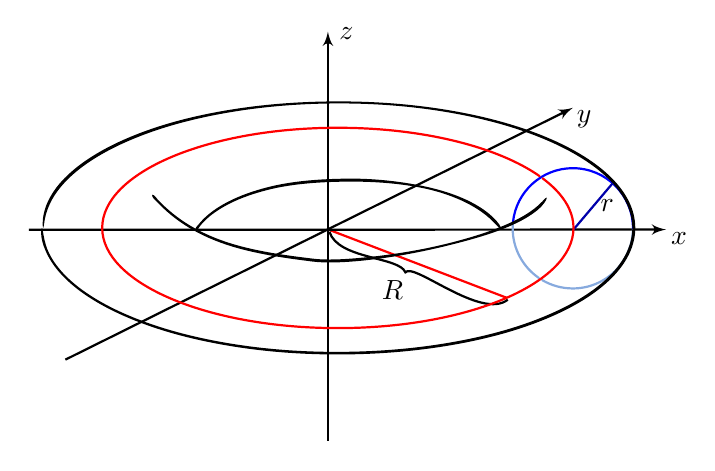
\begin{tikzpicture}[y=0.80pt, x=0.8pt,yscale=-1,scale=0.4, inner sep=0pt, outer sep=0pt]
\begin{scope}[shift={(25.05069,23.8118)}]% layer1
  % path4821
  \path[draw=cff0000,line join=miter,line cap=butt,line width=0.800pt]
    (312.7500,199.4579) -- (514.6288,276.7267);

  % path2584-4-4
  \path[draw=black,line join=miter,line cap=butt,line width=0.800pt,latex'-]
    (312.7500,-23.8118) -- (312.7500,438.9362);

  % path2586-9-9
  \path[draw=black,line join=miter,line cap=butt,line width=0.800pt,-latex']
    (-25.0505,199.9454) -- (694.5362,199.6730);

  % path2582-5-0
  \path[draw=black,line join=miter,line cap=butt,line width=0.800pt,-latex']
    (16.2442,346.6000) -- (589.2275,62.2550);

  \path[draw=black,fill=black,line join=miter,line cap=butt,fill
    opacity=0.000,line width=0.800pt] (314.4993,202.2400) .. controls
    (324.1573,233.4524) and (393.3867,230.1401) .. (400.2468,247.9921) .. controls
    (409.2796,235.9115) and (485.9943,302.4241) .. (515.8186,278.8714);


  % path4894
  \path[draw=c87aade,line cap=round,miter limit=4.00,line width=0.798pt]
    (551.0331,254.3893) .. controls (533.1249,242.1607) and (521.3699,221.5847) ..
    (521.3699,198.2632) .. controls (521.3699,195.9190) and (521.4887,193.6024) ..
    (521.7206,191.3193)(657.1996,198.2632) .. controls (657.1996,235.7716) and
    (626.7931,266.1781) .. (589.2847,266.1781) .. controls (576.6367,266.1781) and
    (564.7962,262.7206) .. (554.6568,256.6993);

  % path4815
  \path[draw=c0000ff,line cap=round,miter limit=4.00,line width=0.798pt]
    (657.1948,198.2604) .. controls (657.1948,160.7521) and (626.7969,130.3542) ..
    (589.2885,130.3542) .. controls (554.1245,130.3542) and (525.2040,157.0764) ..
    (521.7261,191.3229);

  % path4765
  \path[fill=black,nonzero rule] (4.0942,161.0214) .. controls (8.0203,154.9244)
    and (12.7279,149.2724) .. (17.8623,144.0504) .. controls (26.8817,134.8858)
    and (37.2471,127.0373) .. (48.1833,120.0921) .. controls (48.1833,120.0921)
    and (48.1833,120.0921) .. (48.1833,120.0921) .. controls (60.9938,111.9603)
    and (74.6167,105.0935) .. (88.6152,99.0957) .. controls (88.6152,99.0957) and
    (88.6152,99.0957) .. (88.6152,99.0957) .. controls (122.3326,84.6490) and
    (158.0930,75.1580) .. (194.2955,68.5922) .. controls (237.0025,60.8500) and
    (280.4722,57.3540) .. (323.9382,57.2543) .. controls (331.8272,57.2365) and
    (339.7182,57.3306) .. (347.6068,57.5410) .. controls (383.1540,58.4895) and
    (418.6481,61.9091) .. (453.6499,68.2082) .. controls (453.6499,68.2082) and
    (453.6499,68.2082) .. (453.6500,68.2082) .. controls (489.8622,74.7273) and
    (525.6575,84.2038) .. (559.4644,98.6175) .. controls (559.4644,98.6175) and
    (559.4644,98.6175) .. (559.4644,98.6175) .. controls (573.4903,104.5973) and
    (587.1541,111.4455) .. (600.0279,119.5600) .. controls (600.0279,119.5600) and
    (600.0279,119.5601) .. (600.0279,119.5601) .. controls (611.0139,126.4867) and
    (621.4487,134.3243) .. (630.5691,143.4981) .. controls (630.5691,143.4981) and
    (630.5691,143.4981) .. (630.5691,143.4981) .. controls (638.2793,151.2579) and
    (645.0679,159.9958) .. (649.7802,169.7879) .. controls (649.7802,169.7879) and
    (649.7802,169.7879) .. (649.7802,169.7880) .. controls (653.9929,178.5369) and
    (656.4558,188.1668) .. (656.4622,197.8407) .. controls (656.4662,200.3195) and
    (656.3098,202.7962) .. (656.0034,205.2567) .. controls (655.1141,212.3983) and
    (652.9582,219.4019) .. (649.8271,225.9161) .. controls (645.1184,235.7177) and
    (638.3202,244.4593) .. (630.5960,252.2101) .. controls (621.4598,261.3727) and
    (611.0038,269.1838) .. (599.9972,276.0727) .. controls (587.1003,284.1422) and
    (573.4145,290.9296) .. (559.3704,296.8427) .. controls (559.3704,296.8427) and
    (559.3703,296.8427) .. (559.3703,296.8427) .. controls (525.5236,311.0935) and
    (489.7210,320.3650) .. (453.5225,326.7643) .. controls (453.5225,326.7643) and
    (453.5225,326.7643) .. (453.5225,326.7643) .. controls (413.5309,333.8304) and
    (372.9336,337.2307) .. (332.3170,337.7287) .. controls (329.5241,337.7629) and
    (326.7311,337.7828) .. (323.9382,337.7885) .. controls (280.5121,337.8745) and
    (237.0536,334.5341) .. (194.3176,326.9665) .. controls (158.0990,320.5500) and
    (122.2977,311.2277) .. (88.4511,296.9720) .. controls (74.4004,291.0541) and
    (60.7069,284.2682) .. (47.7934,276.2090) .. controls (36.7699,269.3275) and
    (26.2903,261.5284) .. (17.1129,252.3767) .. controls (17.1129,252.3767) and
    (17.1129,252.3767) .. (17.1129,252.3767) .. controls (9.3517,244.6336) and
    (2.5051,235.8944) .. (-2.2720,226.0708) .. controls (-2.9715,224.6329) and
    (-3.6239,223.1707) .. (-4.2261,221.6879) .. controls (-5.6714,217.6951) and
    (-6.6336,214.1519) .. (-7.3308,211.1213) .. controls (-8.0279,208.0907) and
    (-8.4613,205.5690) .. (-8.7952,203.5696) .. controls (-9.1292,201.5701) and
    (-9.3648,200.0912) .. (-9.5950,199.1369) .. controls (-9.8252,198.1827) and
    (-10.0506,197.7531) .. (-10.2810,197.8555) .. controls (-10.5115,197.9578) and
    (-10.7468,198.5931) .. (-10.9124,199.7633) .. controls (-11.0780,200.9335) and
    (-11.1726,202.6403) .. (-11.0487,204.8577) .. controls (-10.9249,207.0750) and
    (-10.5801,209.8050) .. (-9.8216,212.9626) .. controls (-9.0630,216.1201) and
    (-7.8869,219.7075) .. (-6.1009,223.5474) .. controls (-5.5914,224.7573) and
    (-5.0496,225.9528) .. (-4.4769,227.1322) .. controls (0.4492,237.2692) and
    (7.4420,246.2420) .. (15.3468,254.1340) .. controls (15.3468,254.1340) and
    (15.3468,254.1340) .. (15.3468,254.1341) .. controls (24.6852,263.4639) and
    (35.3024,271.3962) .. (46.4384,278.3627) .. controls (59.4829,286.5258) and
    (73.2887,293.3943) .. (87.4312,299.3712) .. controls (121.4919,313.7657) and
    (157.4734,323.1955) .. (193.8295,329.6810) .. controls (236.7354,337.3376) and
    (280.3580,340.7521) .. (323.9382,340.7215) .. controls (325.9403,340.7205) and
    (327.9426,340.7115) .. (329.9449,340.6956) .. controls (371.5117,340.3642) and
    (413.0948,337.0140) .. (454.0738,329.8308) .. controls (454.0738,329.8308) and
    (454.0738,329.8308) .. (454.0738,329.8308) .. controls (490.4483,323.4572) and
    (526.4898,314.1628) .. (560.6420,299.8343) .. controls (560.6420,299.8343) and
    (560.6420,299.8343) .. (560.6420,299.8343) .. controls (574.8177,293.8867) and
    (588.6647,287.0327) .. (601.7531,278.8636) .. controls (601.7532,278.8636) and
    (601.7532,278.8636) .. (601.7532,278.8636) .. controls (612.9244,271.8943) and
    (623.5821,263.9368) .. (632.9577,254.5601) .. controls (632.9577,254.5601) and
    (632.9577,254.5601) .. (632.9577,254.5601) .. controls (640.8943,246.6302) and
    (647.9133,237.5912) .. (652.8511,227.3719) .. controls (655.2634,222.3744) and
    (657.1229,217.0891) .. (658.3142,211.6544) .. controls (659.3034,207.1416) and
    (659.8362,202.5105) .. (659.8368,197.8407) .. controls (659.8185,187.6639) and
    (657.2651,177.5346) .. (652.8090,168.3299) .. controls (647.8903,158.1794) and
    (640.8832,149.1355) .. (632.9082,141.1707) .. controls (623.5802,131.8457) and
    (612.9308,123.8734) .. (601.7202,116.8704) .. controls (601.7202,116.8703) and
    (601.7202,116.8703) .. (601.7202,116.8703) .. controls (588.6821,108.7218) and
    (574.8358,101.8432) .. (560.6343,95.8652) .. controls (526.4577,81.4793) and
    (490.2440,72.1037) .. (454.0932,65.7429) .. controls (417.6836,59.3338) and
    (381.1991,56.0741) .. (345.6564,55.2078) .. controls (338.3783,55.0304) and
    (331.1394,54.9481) .. (323.9382,54.9548) .. controls (301.6471,54.9748) and
    (279.6929,55.8454) .. (258.0216,57.6311) .. controls (236.3503,59.4168) and
    (214.9608,62.1169) .. (193.8000,65.8361) .. controls (175.6371,69.0271) and
    (157.6068,72.9443) .. (139.8187,77.8745) .. controls (122.0305,82.8046) and
    (104.4831,88.7463) .. (87.3112,96.0279) .. controls (73.2621,101.9855) and
    (59.4655,108.8759) .. (46.3461,117.1721) .. controls (35.3262,124.1380) and
    (24.7431,132.1196) .. (15.4059,141.6062) .. controls (13.3144,143.7298) and
    (11.2855,145.9346) .. (9.3425,148.2227) .. controls (7.1403,150.8344) and
    (4.7178,153.9819) .. (2.4179,157.4921) .. controls (0.1179,161.0023) and
    (-2.0517,164.8770) .. (-3.8341,168.8587) .. controls (-5.9022,173.4802) and
    (-7.3929,178.2444) .. (-8.2673,182.5219) .. controls (-9.1417,186.7994) and
    (-9.4124,190.5799) .. (-9.3867,193.2980) .. controls (-9.3609,196.0161) and
    (-9.0758,197.6742) .. (-8.8087,197.8288) .. controls (-8.6752,197.9061) and
    (-8.5421,197.6089) .. (-8.3901,196.8882) .. controls (-8.2380,196.1675) and
    (-8.0681,195.0227) .. (-7.7982,193.4117) .. controls (-7.3733,189.8346) and
    (-6.6453,185.9498) .. (-5.5265,181.9959) .. controls (-4.4076,178.0420) and
    (-2.8986,174.0225) .. (-1.0632,170.1926) .. controls (0.4755,166.9786) and
    (2.2306,163.8924) .. (4.0942,161.0214) -- cycle;

  % path4767
  \path[fill=black] (503.5147,190.4138) .. controls (497.8712,183.8617) and
    (490.9723,178.4847) .. (483.7352,173.9957) .. controls (471.3080,166.2605) and
    (457.6720,160.7741) .. (443.7823,156.5342) .. controls (443.7823,156.5342) and
    (443.7823,156.5342) .. (443.7823,156.5342) .. controls (436.9991,154.4611) and
    (430.1320,152.6893) .. (423.2065,151.1932) .. controls (413.5305,149.1028) and
    (403.7704,147.4121) .. (393.9732,146.0538) .. controls (375.7698,143.5289) and
    (357.3896,142.1734) .. (339.0053,142.1536) .. controls (339.0053,142.1536) and
    (339.0053,142.1536) .. (339.0053,142.1536) .. controls (337.2641,142.1516) and
    (335.5228,142.1616) .. (333.7817,142.1842) .. controls (316.9981,142.4009) and
    (300.2056,143.1456) .. (283.4986,145.0127) .. controls (270.3235,146.4842) and
    (257.1817,148.6495) .. (244.3204,151.9665) .. controls (240.2713,153.0108) and
    (236.2452,154.1446) .. (232.2474,155.3753) .. controls (232.2474,155.3753) and
    (232.2474,155.3753) .. (232.2474,155.3753) .. controls (217.6503,159.8639) and
    (203.3321,165.6502) .. (190.3143,173.7009) .. controls (181.2106,179.3207) and
    (172.6670,186.1743) .. (166.0947,194.5868) .. controls (164.5593,196.0240) and
    (163.7269,197.3380) .. (163.3830,198.3144) .. controls (163.0391,199.2907) and
    (163.1791,199.9337) .. (163.5894,200.1493) .. controls (163.9997,200.3650) and
    (164.6770,200.1593) .. (165.4689,199.4785) .. controls (166.2608,198.7979) and
    (167.1659,197.6463) .. (168.1306,195.9335) .. controls (174.4871,187.9341) and
    (182.7889,181.3854) .. (191.6622,175.9466) .. controls (204.4670,168.1127) and
    (218.6043,162.5029) .. (233.0689,158.1311) .. controls (233.0689,158.1311) and
    (233.0689,158.1311) .. (233.0689,158.1311) .. controls (236.8459,156.9903) and
    (240.6492,155.9367) .. (244.4743,154.9638) .. controls (257.4013,151.6759) and
    (270.6277,149.5704) .. (283.8983,148.1578) .. controls (300.0177,146.4431) and
    (316.2116,145.7684) .. (332.3976,145.5703) .. controls (334.5806,145.5436) and
    (336.7789,145.5290) .. (338.9901,145.5275) .. controls (356.7946,145.5161) and
    (375.4462,146.3916) .. (393.6247,148.5981) .. controls (403.7099,149.8230) and
    (413.6506,151.4390) .. (423.1723,153.5209) .. controls (430.0115,155.0163) and
    (436.6178,156.8175) .. (443.0424,158.9009) .. controls (449.9488,161.1424) and
    (456.6621,163.6950) .. (463.1516,166.6440) .. controls (469.6412,169.5929) and
    (475.9075,172.9341) .. (481.9343,176.8127) .. controls (487.8903,180.6590) and
    (493.6689,185.0411) .. (498.7303,190.2674) .. controls (499.6598,191.1990) and
    (500.8405,192.3751) .. (502.0221,193.5962) .. controls (503.2037,194.8173) and
    (504.3847,196.0858) .. (505.3941,197.1282) .. controls (506.4035,198.1707) and
    (507.2480,198.9842) .. (507.8010,199.2244) .. controls (508.3540,199.4647) and
    (508.6307,199.1213) .. (508.3823,197.8783) .. controls (507.8987,196.6397) and
    (507.1614,195.3289) .. (506.3021,194.0554) .. controls (505.4429,192.7820) and
    (504.4623,191.5464) .. (503.5147,190.4138) -- cycle;

  % path4769
  \path[fill=black] (550.8815,171.8191) .. controls (547.7848,174.6969) and
    (544.3898,177.2968) .. (540.8425,179.7088) .. controls (540.8425,179.7088) and
    (540.8425,179.7088) .. (540.8425,179.7088) .. controls (531.9167,185.7778) and
    (522.1202,190.6146) .. (512.0785,194.8890) .. controls (512.0785,194.8890) and
    (512.0785,194.8890) .. (512.0785,194.8890) .. controls (500.2871,199.9044) and
    (488.1202,204.0733) .. (475.8070,207.7889) .. controls (475.8070,207.7889) and
    (475.8070,207.7889) .. (475.8070,207.7889) .. controls (466.1032,210.7166) and
    (456.3052,213.3511) .. (446.4483,215.7775) .. controls (442.7624,216.6848) and
    (439.0654,217.5507) .. (435.3595,218.3795) .. controls (408.7503,224.3306) and
    (381.7290,228.4611) .. (354.5810,231.1344) .. controls (354.5810,231.1344) and
    (354.5810,231.1344) .. (354.5810,231.1344) .. controls (347.3015,231.8511) and
    (340.0135,232.4617) .. (332.7191,232.9084) .. controls (328.7181,233.1534) and
    (324.7138,233.3274) .. (320.7082,233.4219) .. controls (312.2469,233.6196) and
    (303.7872,233.5515) .. (295.4696,232.5124) .. controls (280.8345,230.6907) and
    (266.2182,228.8636) .. (251.7388,226.4286) .. controls (240.7173,224.5745) and
    (229.7609,222.3905) .. (218.9420,219.7250) .. controls (213.9261,218.4892) and
    (208.9448,217.1265) .. (204.0080,215.6158) .. controls (204.0080,215.6158) and
    (204.0080,215.6158) .. (204.0080,215.6158) .. controls (187.5834,210.5888) and
    (171.6369,203.9105) .. (156.9358,195.0714) .. controls (143.3859,186.9268) and
    (130.9352,176.9082) .. (120.1489,165.3066) .. controls (118.5930,163.1540) and
    (117.2761,161.7443) .. (116.2506,160.9574) .. controls (115.2250,160.1704) and
    (114.4931,160.0082) .. (114.1767,160.3493) .. controls (113.8602,160.6905) and
    (113.9617,161.5373) .. (114.6376,162.7356) .. controls (115.3136,163.9340) and
    (116.5666,165.4857) .. (118.5515,167.1731) .. controls (129.3987,178.9002) and
    (141.9136,189.0500) .. (155.5475,197.3285) .. controls (170.4323,206.3642) and
    (186.5568,213.2096) .. (203.1469,218.3614) .. controls (203.1469,218.3614) and
    (203.1469,218.3614) .. (203.1469,218.3614) .. controls (207.8953,219.8362) and
    (212.6818,221.1750) .. (217.4974,222.3961) .. controls (228.6444,225.2228) and
    (239.9227,227.5340) .. (251.2521,229.4878) .. controls (265.8205,232.0008) and
    (280.4789,233.8936) .. (295.0992,235.7621) .. controls (295.0992,235.7621) and
    (295.0992,235.7621) .. (295.0992,235.7621) .. controls (303.6599,236.8504) and
    (312.2742,236.9502) .. (320.7933,236.7650) .. controls (320.7933,236.7650) and
    (320.7933,236.7650) .. (320.7933,236.7650) .. controls (324.2275,236.6918) and
    (327.6587,236.5604) .. (331.0856,236.3760) .. controls (338.9207,235.9542) and
    (346.8843,235.2727) .. (354.9065,234.4163) .. controls (368.4281,232.9734) and
    (382.1431,231.0393) .. (395.7358,228.7017) .. controls (409.3284,226.3642) and
    (422.7982,223.6242) .. (435.8526,220.6350) .. controls (439.8025,219.7306) and
    (443.7150,218.8016) .. (447.5809,217.8491) .. controls (457.4764,215.4110) and
    (467.0894,212.9113) .. (476.5247,210.2095) .. controls (489.0532,206.6225) and
    (501.2925,202.6935) .. (513.2962,197.8059) .. controls (523.3820,193.7024) and
    (533.3845,188.9383) .. (542.7495,182.6056) .. controls (545.2281,180.9295) and
    (547.6607,179.1337) .. (549.9982,177.1830) .. controls (551.0667,176.2710) and
    (552.3168,175.1093) .. (553.5462,173.8214) .. controls (554.7800,172.5297) and
    (555.9914,171.1051) .. (557.0015,169.7214) .. controls (558.0117,168.3376) and
    (558.8191,166.9970) .. (559.3263,165.9184) .. controls (559.8334,164.8397) and
    (560.0466,164.0285) .. (559.9146,163.6894) .. controls (559.7826,163.3503) and
    (559.3168,163.4890) .. (558.3713,164.2063) .. controls (557.3373,165.2692) and
    (556.2211,166.4906) .. (555.0337,167.7329) .. controls (553.8464,168.9752) and
    (552.5894,170.2387) .. (551.3413,171.3974) .. controls (551.1878,171.5397) and
    (551.0344,171.6803) .. (550.8815,171.8191) -- cycle;

  % path4819
  \path[draw=c0000aa,fill=black,line join=miter,line cap=butt,fill
    opacity=0.000,line width=0.800pt] (589.9942,199.7248) -- (634.2774,147.3889);

  % path4898
  \path[draw=cff0000,line cap=round,miter limit=4.00,line width=0.798pt]
    (551.6880,139.3176) .. controls (505.0564,106.5995) and (420.5044,84.7345) ..
    (323.9382,84.7345) .. controls (176.9796,84.7345) and (57.8460,135.3739) ..
    (57.8460,197.8407) .. controls (57.8460,260.3076) and (176.9796,310.9470) ..
    (323.9382,310.9470) .. controls (470.8968,310.9470) and (590.0304,260.3076) ..
    (590.0304,197.8407) .. controls (590.0304,177.4669) and (577.3573,158.3512) ..
    (555.1792,141.8403);

  % path4823
  % text4847
  \path[fill=black] (373.61691,278.13907) node[above right] (text4847) {$R$};

  % text4851
  \path[fill=black] (620.76501,179.84439) node[above right] (text4851) {$r$};

  % text4855
  \path[fill=black] (700.42676,216.76456) node[above right] (text4855) {$x$};

  % text4859
  \path[fill=black] (593.76367,84.783592) node[above right] (text4859) {$y$};

  % text4863
  \path[fill=black] (325.72787,-14.842139) node[above right] (text4863) {$z$};

\end{scope}

\end{tikzpicture}


\end{center}

\end{itemize}
\end{przyklad}

\end{frame}
%%%%%%next-slide%%%%%
\mode<all>{\lowsection{Powierzchnie prostokreślne}}
\begin{frame}[<+->]

\begin{definicja}
\textbf{Powierzchnią prostokreślną} nazywamy powierzchnię o parametryzacji\[x(s,t)=\alpha(s)+t\beta(s),\] gdzie $\alpha$ i $\beta$ są krzywymi w przestrzeni $\R^3$. $\alpha$ nazywa się potocznie kierownicą, $\beta$ - ruletą.

\begin{center}

\definecolor{c0000ff}{RGB}{0,0,255}


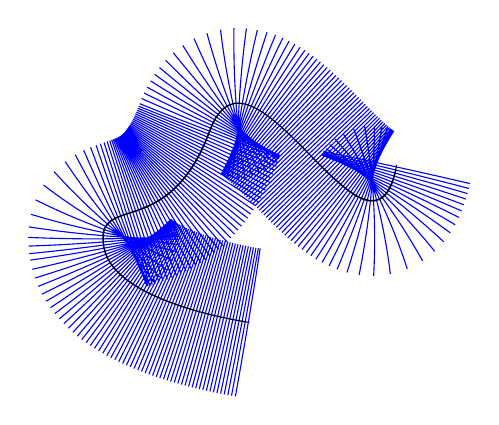
\begin{tikzpicture}[y=0.80pt, x=0.8pt,yscale=-1, scale=0.22, inner sep=0pt, outer sep=0pt]
\begin{scope}[shift={(167.02692,-168.50889)}]% layer1
  % path1158
  \path[draw=c0000ff] (309.1030,620.7084) .. controls (309.0594,621.0244) and
    (309.0156,621.3404) .. (308.9717,621.6563) .. controls (308.8428,622.5836) and
    (308.7126,623.5106) .. (308.5813,624.4375) .. controls (308.5813,624.4375) and
    (308.5813,624.4375) .. (308.5813,624.4375) .. controls (308.0615,628.1053) and
    (307.5228,631.7703) .. (306.9682,635.4330) -- (306.9682,635.4330) .. controls
    (304.8299,649.8862) and (302.5848,664.3234) .. (300.2762,678.7510) --
    (300.2762,678.7510) .. controls (291.2681,735.0505) and (281.7100,791.2638) ..
    (271.9304,847.4392) .. controls (271.9304,847.4392) and (271.9304,847.4392) ..
    (271.9304,847.4392) .. controls (267.4674,873.0745) and (262.9491,898.7007) ..
    (258.3796,924.3182)(305.4418,620.1277) .. controls (287.8063,721.2065) and
    (269.3767,822.1513) .. (250.3937,922.9955)(300.5367,619.2968) .. controls
    (281.8317,720.1849) and (262.5843,820.9746) ..
    (242.8185,921.6668)(295.3954,618.3821) .. controls (275.8800,719.1158) and
    (255.8466,819.7521) .. (235.3194,920.2923)(290.2073,617.4160) .. controls
    (269.9186,717.9973) and (249.1364,818.4824) ..
    (227.8848,918.8726)(284.9723,616.4008) .. controls (263.9475,716.8317) and
    (242.4536,817.1678) .. (220.5146,917.4101)(279.6904,615.3387) .. controls
    (257.9665,715.6215) and (235.7979,815.8106) ..
    (213.2089,915.9072)(274.3592,614.2302) .. controls (251.9707,714.3638) and
    (229.1759,814.4152) .. (205.9644,914.3776)(269.0039,613.0704) .. controls
    (245.9939,713.0712) and (222.5669,812.9829) ..
    (198.7123,912.7983)(263.6816,611.8865) .. controls (240.0338,711.7438) and
    (215.9583,811.5048) .. (191.4444,911.1625)(258.3929,610.6775) .. controls
    (234.0911,710.3804) and (209.3508,809.9799) ..
    (184.1613,909.4691)(253.1385,609.4423) .. controls (228.1664,708.9800) and
    (202.7450,808.4072) .. (176.8637,907.7171)(247.9190,608.1800) .. controls
    (222.2604,707.5416) and (196.1416,806.7857) ..
    (169.5523,905.9054)(242.7353,606.8896) .. controls (216.3737,706.0642) and
    (189.5414,805.1143) .. (162.2276,904.0330)(237.5878,605.5698) .. controls
    (210.5071,704.5467) and (182.9449,803.3921) ..
    (154.8905,902.0988)(232.4773,604.2199) .. controls (204.6612,702.9882) and
    (176.3528,801.6179) .. (147.5415,900.1019)(227.4044,602.8386) .. controls
    (198.8366,701.3875) and (169.7658,799.7907) ..
    (140.1813,898.0413)(222.3698,601.4251) .. controls (193.0341,699.7437) and
    (163.1846,797.9096) .. (132.8106,895.9158)(217.3742,599.9782) .. controls
    (187.2543,698.0557) and (156.6098,795.9734) ..
    (125.4300,893.7244)(212.4182,598.4969) .. controls (181.4978,696.3225) and
    (150.0420,793.9813) .. (118.0403,891.4662)(207.5025,596.9802) .. controls
    (175.7653,694.5430) and (143.4820,791.9320) ..
    (110.6420,889.1400)(202.6277,595.4270) .. controls (170.0576,692.7163) and
    (136.9305,789.8246) .. (103.2359,886.7449)(197.7946,593.8364) .. controls
    (166.3050,685.2397) and (134.3113,776.4760) .. (101.8048,867.5395) .. controls
    (99.8123,873.1202) and (97.8178,878.7003) ..
    (95.8213,884.2798)(193.0193,592.2106) .. controls (158.7350,688.9213) and
    (123.8539,785.4324) .. (88.3431,881.7205)(188.3485,590.5748) .. controls
    (153.1431,686.9637) and (117.3077,783.1293) ..
    (80.8093,879.0484)(183.7750,588.9315) .. controls (147.5983,684.9623) and
    (110.7583,780.7463) .. (73.2219,876.2600)(179.3013,587.2775) .. controls
    (142.1029,682.9141) and (104.2079,778.2801) ..
    (65.5833,873.3523)(174.9294,585.6098) .. controls (136.6591,680.8158) and
    (97.6588,775.7277) .. (57.8957,870.3221)(170.6616,583.9250) .. controls
    (131.2690,678.6643) and (91.1132,773.0858) ..
    (50.1614,867.1662)(166.5001,582.2200) .. controls (125.9350,676.4563) and
    (84.5734,770.3512) .. (42.3824,863.8814)(162.4473,580.4917) .. controls
    (120.6593,674.1888) and (78.0416,767.5208) ..
    (34.5612,860.4645)(158.5052,578.7368) .. controls (123.4450,654.5561) and
    (87.8126,730.1178) .. (51.5904,805.4092) .. controls (43.3251,822.5930) and
    (35.0295,839.7636) .. (26.7030,856.9207)(154.6704,576.9289) .. controls
    (110.2909,669.4488) and (65.0178,761.5753) ..
    (18.7825,853.2383)(151.0046,575.1392) .. controls (105.2373,667.0154) and
    (58.5072,758.4271) .. (10.7455,849.3042)(147.5425,573.4170) .. controls
    (100.2829,664.5408) and (51.9912,755.1291) ..
    (2.5988,845.1118)(144.2908,571.7557) .. controls (95.4345,662.0186) and
    (45.4768,751.6748) .. (-5.6511,840.6544)(141.2563,570.1486) .. controls
    (90.6987,659.4419) and (38.9705,748.0575) ..
    (-13.9972,835.9254)(138.4456,568.5892) .. controls (86.0824,656.8041) and
    (32.4791,744.2704) .. (-22.4329,830.9180)(135.8656,567.0706) .. controls
    (81.5922,654.0987) and (26.0093,740.3071) ..
    (-30.9515,825.6258)(133.5230,565.5862) .. controls (77.2348,651.3189) and
    (19.5679,736.1608) .. (-39.5462,820.0419)(131.4244,564.1295) .. controls
    (122.9728,576.3319) and (114.4909,588.5142) .. (105.9785,600.6761) .. controls
    (55.6739,672.5360) and (4.2793,743.7639) ..
    (-48.2703,814.2121)(129.6830,562.6659) .. controls (69.0142,645.5297) and
    (6.7656,727.3247) .. (-57.1667,807.8149)(128.2962,561.5710) .. controls
    (65.1880,642.6722) and (0.3953,722.4656) ..
    (-66.1861,800.7152)(127.2794,560.8557) .. controls (61.5751,639.8302) and
    (-5.9186,717.2580) .. (-75.3058,792.9030)(126.6551,560.5098) .. controls
    (58.1980,636.9936) and (-12.1534,711.6917) ..
    (-84.5032,784.3681)(126.4462,560.5231) .. controls (55.0795,634.1522) and
    (-18.2864,705.7566) .. (-93.7554,775.1004)(126.6753,560.8854) .. controls
    (52.2423,631.2958) and (-24.2948,699.4425) ..
    (-103.0398,765.0896)(127.3653,561.5867) .. controls (49.7091,628.4143) and
    (-30.1559,692.7393) .. (-112.3337,754.3257)(128.5440,562.7167) .. controls
    (47.5015,625.6367) and (-35.8692,685.6386) ..
    (-121.5249,742.2759)(130.0534,564.7940) .. controls (45.5321,623.0279) and
    (-41.2725,677.8917) .. (-130.3174,728.9387)(131.7947,567.6827) .. controls
    (43.8675,620.5443) and (-46.2984,669.5836) ..
    (-138.6596,714.3540)(133.8112,571.3867) .. controls (99.1438,589.1659) and
    (64.1597,606.3284) .. (28.8614,622.8496) .. controls (-28.7604,649.8265) and
    (-87.2286,675.0569) .. (-146.4628,698.4599)(135.9782,576.0021) .. controls
    (41.4656,616.0080) and (-55.0339,651.2584) ..
    (-153.1837,681.4141)(137.8573,581.2772) .. controls (40.5538,613.8681) and
    (-58.3950,641.3610) .. (-158.6520,663.4165)(139.4535,587.1831) .. controls
    (43.9921,610.8244) and (-52.6672,629.4649) .. (-150.2277,642.8056) .. controls
    (-154.4190,643.4403) and (-158.6112,644.0705) ..
    (-162.8043,644.6961)(140.3893,591.1799) .. controls (39.0938,607.6377) and
    (-62.7226,621.3685) .. (-164.9079,631.3946)(140.5182,592.5003) .. controls
    (38.5483,604.3083) and (-63.7865,612.3995) ..
    (-166.3340,615.7961)(140.6768,596.0430) .. controls (46.2455,601.2594) and
    (-48.3633,602.4730) .. (-143.0303,598.9170) .. controls (-151.0210,598.6127)
    and (-159.0122,598.2728) .. (-167.0034,597.8966)(140.9234,602.0972) ..
    controls (38.2537,600.1586) and (-64.3906,592.1894) ..
    (-165.8500,576.3357)(139.7648,612.2714) .. controls (37.8133,600.2292) and
    (-62.9344,580.2822) .. (-161.3185,550.5766)(136.6600,626.9580) .. controls
    (37.0773,602.1105) and (-59.9147,566.8393) ..
    (-151.8771,520.8271)(129.4967,645.2472) .. controls (35.2189,604.4561) and
    (-53.9982,552.9257) .. (-135.7157,490.3386)(117.6713,664.5314) .. controls
    (32.5203,607.0602) and (-44.7645,538.9764) ..
    (-114.0684,462.9178)(104.0208,680.0088) .. controls (34.0925,610.9558) and
    (-28.5288,534.6274) .. (-83.7424,453.3364) .. controls (-86.2225,449.7021) and
    (-88.6890,446.0583) .. (-91.1420,442.4050)(91.3944,690.0081) .. controls
    (30.6842,607.3243) and (-22.6854,519.5240) ..
    (-70.3571,428.4569)(82.7478,695.5728) .. controls (38.6503,617.2760) and
    (-1.0998,536.4906) .. (-37.6043,454.4575) .. controls (-42.8056,442.7780) and
    (-47.9424,431.0695) .. (-53.0169,419.3333)(78.1949,697.6988) .. controls
    (35.5604,604.4004) and (-3.0855,509.3225) ..
    (-38.9826,413.1352)(76.9749,698.2967) .. controls (39.7707,602.6706) and
    (5.2982,505.9405) .. (-27.6826,408.7764)(78.7636,697.6024) .. controls
    (45.0450,600.6976) and (12.6588,503.3382) ..
    (-18.9061,405.6994)(82.6027,696.2750) .. controls (50.6471,598.7790) and
    (19.5060,501.0046) .. (-11.3315,403.1272)(87.6428,694.6073) .. controls
    (56.6619,596.7824) and (25.9777,498.8554) ..
    (-4.9208,401.0016)(93.8667,692.5501) .. controls (63.0722,594.6586) and
    (32.0566,496.8413) .. (0.3088,399.2734)(101.2574,690.0541) .. controls
    (69.8609,592.3582) and (37.7255,494.9129) ..
    (4.3402,397.8933)(109.7786,687.0807) .. controls (76.9412,589.8688) and
    (42.9111,493.0305) .. (7.5578,396.6728)(118.7282,683.8027) .. controls
    (84.0071,587.1997) and (47.9609,491.0782) ..
    (10.4591,395.5455)(127.9292,680.1484) .. controls (91.1221,584.3169) and
    (52.8576,489.0751) .. (13.0052,394.5303)(137.3711,676.1050) .. controls
    (98.2759,581.2079) and (57.5909,487.0087) ..
    (15.1856,393.6145)(147.0436,671.6600) .. controls (105.4581,577.8602) and
    (62.1504,484.8664) .. (16.9900,392.7857)(156.9362,666.8009) .. controls
    (112.6582,574.2612) and (66.5256,482.6356) ..
    (18.4079,392.0313)(167.0386,661.5152) .. controls (157.6862,643.4504) and
    (148.2557,625.4258) .. (138.7460,607.4423) .. controls (100.2810,534.7091) and
    (60.5342,462.6756) .. (19.5303,391.3700)(177.1110,655.7619) .. controls
    (126.8966,566.2579) and (74.7269,477.8869) ..
    (20.6503,390.7031)(186.9541,649.6862) .. controls (133.7827,561.9110) and
    (78.7047,475.3239) .. (21.7684,389.9792)(196.5702,643.3056) .. controls
    (140.5151,557.3434) and (82.6021,472.6243) ..
    (22.8794,389.2028)(205.9539,636.6247) .. controls (147.0884,552.5596) and
    (86.4138,469.7929) .. (23.9780,388.3787)(215.1002,629.6482) .. controls
    (153.4976,547.5645) and (90.1346,466.8342) ..
    (25.0591,387.5115)(224.0037,622.3808) .. controls (159.7374,542.3626) and
    (93.7593,463.7529) .. (26.1174,386.6060)(232.6592,614.8271) .. controls
    (172.5674,544.8378) and (111.1319,476.0307) .. (48.3877,408.4455) .. controls
    (41.3272,400.8367) and (34.2510,393.2433) ..
    (27.1591,385.6651)(240.9868,607.0151) .. controls (171.6195,531.3864) and
    (100.7198,457.2495) .. (28.3693,384.5812)(248.8976,599.0923) .. controls
    (177.2296,525.7022) and (104.1120,453.7806) ..
    (29.6262,383.3042)(256.4799,591.0880) .. controls (182.6371,519.9019) and
    (107.4272,450.1610) .. (30.9319,381.8420)(263.7360,583.0100) .. controls
    (187.8441,513.9934) and (110.6678,446.3986) ..
    (32.2887,380.2024)(270.6681,574.8662) .. controls (192.8529,507.9845) and
    (113.8360,442.5013) .. (33.6989,378.3934)(277.2785,566.6645) .. controls
    (197.6659,501.8831) and (116.9341,438.4769) ..
    (35.1648,376.4227)(283.5696,558.4128) .. controls (202.2852,495.6972) and
    (119.9644,434.3334) .. (36.6887,374.2983)(289.5436,550.1188) .. controls
    (206.7132,489.4344) and (122.9291,430.0785) ..
    (38.2728,372.0280)(295.2027,541.7906) .. controls (210.9522,483.1028) and
    (125.8306,425.7202) .. (39.9194,369.6196)(300.5494,533.4358) .. controls
    (299.5102,532.7467) and (298.4709,532.0578) .. (297.4315,531.3691) .. controls
    (212.8974,475.3829) and (127.6210,420.6097) ..
    (41.6400,367.0145)(305.5918,525.1696) .. controls (218.8882,470.3270) and
    (131.4631,416.6911) .. (43.3554,364.2255)(310.4294,516.9213) .. controls
    (222.6378,463.8854) and (134.1642,412.0196) ..
    (45.0475,361.2872)(315.0663,508.6937) .. controls (226.2471,457.4092) and
    (136.7853,407.2579) .. (46.7201,358.2033)(319.5059,500.4906) .. controls
    (229.7194,450.9020) and (139.3300,402.4098) ..
    (48.3765,354.9775)(323.7516,492.3158) .. controls (233.0584,444.3676) and
    (141.8016,397.4790) .. (50.0203,351.6136)(327.8072,484.1730) .. controls
    (236.2675,437.8098) and (144.2038,392.4694) ..
    (51.6551,348.1153)(331.6761,476.0659) .. controls (239.3503,431.2322) and
    (146.5401,387.3845) .. (53.2843,344.4864)(335.3618,467.9983) .. controls
    (242.3103,424.6387) and (148.8140,382.2283) ..
    (54.9116,340.7307)(338.8679,459.9740) .. controls (245.1512,418.0330) and
    (151.0290,377.0044) .. (56.5404,336.8517)(342.1979,451.9966) .. controls
    (247.8763,411.4187) and (153.1888,371.7165) ..
    (58.1743,332.8534)(345.3553,444.0700) .. controls (250.4892,404.7998) and
    (155.2967,366.3684) .. (59.8168,328.7394)(348.3437,436.1979) .. controls
    (280.0201,408.9559) and (211.5492,382.1257) .. (142.9454,355.6940) .. controls
    (115.8502,345.0820) and (88.7931,334.3260) ..
    (61.7824,323.4179)(350.2631,431.5653) .. controls (254.7090,393.9996) and
    (159.7398,354.5367) .. (65.7322,312.8175)(350.8229,430.4755) .. controls
    (256.3749,389.8530) and (162.8941,346.9705) ..
    (70.7572,301.4687)(350.7395,430.3149) .. controls (257.9820,386.0885) and
    (166.5739,339.2393) .. (76.8921,289.4079)(350.0476,431.1197) .. controls
    (259.5650,382.7424) and (170.8141,331.3793) ..
    (84.1718,276.6712)(348.7822,432.9262) .. controls (261.1589,379.8508) and
    (175.6496,323.4267) .. (92.6312,263.2949)(346.9781,435.7705) .. controls
    (279.7859,389.2190) and (214.1843,340.3029) .. (150.3647,288.8394) .. controls
    (134.2471,275.8166) and (118.2583,262.6231) ..
    (102.4077,249.2560)(344.1611,439.9047) .. controls (264.0226,375.7530) and
    (187.2940,307.3362) .. (115.1282,234.3013)(339.0052,445.4396) .. controls
    (264.6884,374.6752) and (194.9495,299.2910) ..
    (130.9417,218.9341)(331.5901,452.2634) .. controls (264.8191,374.3411) and
    (203.9278,291.3421) .. (150.3333,203.6796)(321.3286,459.5434) .. controls
    (264.2675,374.1995) and (214.5198,284.2005) ..
    (173.5026,189.9597)(308.2108,466.5650) .. controls (263.0257,374.3796) and
    (226.8022,278.0063) .. (199.9454,178.7864)(293.2764,471.9941) .. controls
    (261.9414,374.2378) and (239.9751,273.6525) ..
    (227.7823,171.5797)(277.7583,475.1671) .. controls (260.9904,373.8918) and
    (253.8467,271.2910) .. (255.3896,168.5164)(263.7043,476.1555) .. controls
    (261.0723,373.5524) and (267.1124,270.7877) ..
    (280.8869,169.0130)(252.0321,475.2232) .. controls (262.1021,373.1157) and
    (279.5528,272.1223) .. (303.3566,172.4155)(243.1067,473.6252) .. controls
    (263.8430,373.3656) and (290.9193,274.3925) ..
    (323.3081,176.8783)(236.4277,472.2071) .. controls (266.2480,374.0465) and
    (301.3675,277.3445) .. (340.7590,182.2739)(231.9781,470.8701) .. controls
    (269.3000,375.0591) and (310.8805,280.8793) ..
    (355.6923,188.5032)(229.7341,469.5372) .. controls (272.9390,376.4314) and
    (319.3376,284.9398) .. (368.5502,194.9447)(228.7771,468.9611) .. controls
    (276.6209,378.2759) and (327.2744,289.0849) ..
    (380.3580,201.2704)(228.5578,468.9153) .. controls (280.4587,380.4644) and
    (334.7851,293.3876) .. (391.1577,207.5672)(229.0875,469.3631) .. controls
    (284.4635,382.9601) and (341.8810,297.8111) ..
    (400.9606,213.7985)(230.3775,470.2677) .. controls (288.6465,385.7262) and
    (348.5731,302.3188) .. (409.7778,219.9276)(232.4389,471.5926) .. controls
    (233.9256,469.5590) and (235.4130,467.5260) .. (236.9012,465.4936) .. controls
    (296.0136,384.7168) and (356.3770,304.8817) ..
    (417.8716,225.9154)(234.8014,473.3024) .. controls (297.2617,391.9228) and
    (360.9096,311.4549) .. (425.6159,231.8200)(237.3740,475.3048) .. controls
    (301.5625,395.2804) and (366.8082,316.0877) ..
    (432.9820,237.6480)(240.1674,477.5864) .. controls (305.8870,398.7944) and
    (372.5333,320.7542) .. (439.9774,243.3871)(243.1893,480.1350) .. controls
    (310.2428,402.4526) and (378.0926,325.4420) ..
    (446.6098,249.0246)(246.4471,482.9379) .. controls (314.6372,406.2423) and
    (383.4934,330.1386) .. (452.8865,254.5480)(249.9330,485.9785) .. controls
    (319.0505,410.1430) and (388.7360,334.8284) ..
    (458.9341,259.9877)(253.4969,489.1888) .. controls (323.4435,414.1256) and
    (393.9021,339.5356) .. (464.8172,265.3722)(257.1452,492.5546) .. controls
    (327.8363,418.1909) and (398.9833,344.2530) ..
    (470.5307,270.6942)(260.8826,496.0706) .. controls (332.2334,422.3337) and
    (403.9841,348.9751) .. (476.0791,275.9482)(264.7133,499.7313) .. controls
    (336.6393,426.5485) and (408.9089,353.6966) ..
    (481.4668,281.1289)(268.6421,503.5313) .. controls (341.0584,430.8300) and
    (413.7623,358.4121) .. (486.6983,286.2309)(272.6732,507.4653) .. controls
    (289.6882,490.5740) and (306.7158,473.6956) .. (323.7554,456.8295) .. controls
    (379.6404,401.5094) and (435.6601,346.3249) ..
    (491.7984,291.2601)(276.7701,511.5060) .. controls (349.9252,439.5567) and
    (423.2820,367.8107) .. (496.8052,296.2327)(280.9264,515.6444) .. controls
    (354.3678,443.9875) and (427.9754,372.4980) ..
    (501.7137,301.1409)(285.1492,519.8791) .. controls (358.8233,448.4598) and
    (432.6277,377.1723) .. (506.5272,305.9813)(289.4420,524.2067) .. controls
    (363.2948,452.9703) and (437.2423,381.8301) ..
    (511.2492,310.7505)(293.8081,528.6237) .. controls (367.7858,457.5156) and
    (441.8225,386.4678) .. (515.8829,315.4450)(298.2509,533.1267) .. controls
    (372.2997,462.0922) and (446.3718,391.0822) ..
    (520.4319,320.0614)(302.7679,537.7085) .. controls (376.8337,466.6928) and
    (450.8960,395.6719) .. (524.9159,324.6071)(307.3590,542.3654) .. controls
    (381.3999,471.3213) and (455.3980,400.2329) ..
    (529.3146,329.0614)(312.0449,547.1060) .. controls (386.0017,475.9738) and
    (459.8765,404.7580) .. (533.6305,333.4201)(316.8292,551.9267) .. controls
    (390.6428,480.6465) and (464.3351,409.2435) ..
    (537.8674,337.6793)(321.7158,556.8237) .. controls (395.3269,485.3356) and
    (468.7776,413.6856) .. (542.0290,341.8352)(326.7083,561.7932) .. controls
    (400.0578,490.0373) and (473.2077,418.0804) ..
    (546.1190,345.8840)(331.8104,566.8314) .. controls (350.1025,548.7761) and
    (368.3795,530.7058) .. (386.6409,512.6198) .. controls (441.2827,458.4978) and
    (495.7966,404.2421) .. (550.1518,349.8270)(337.0188,571.9342) .. controls
    (409.6777,499.4683) and (482.0533,426.7178) ..
    (554.0722,353.6217)(342.4170,577.1440) .. controls (414.6114,504.2107) and
    (486.4483,430.9309) .. (557.8546,357.2436)(348.0186,582.4581) .. controls
    (419.6366,508.9626) and (490.8232,435.0588) ..
    (561.5050,360.6857)(353.8296,587.8693) .. controls (424.7594,513.7170) and
    (495.1836,439.0944) .. (565.0290,363.9407)(359.8557,593.3707) .. controls
    (429.9854,518.4667) and (499.5355,443.0306) ..
    (568.4326,367.0016)(366.1029,598.9550) .. controls (388.1304,574.8486) and
    (410.0916,550.6821) .. (431.9843,526.4535) .. controls (478.8786,474.5457) and
    (525.4892,422.3617) .. (571.7504,369.8630)(372.5679,604.6319) .. controls
    (440.7923,527.9462) and (508.2629,450.5816) ..
    (574.7726,372.4170)(379.5430,610.4998) .. controls (446.5241,532.7106) and
    (512.5420,454.1194) .. (577.3899,374.6054)(387.0745,616.5489) .. controls
    (452.4957,537.4672) and (516.7444,457.4606) ..
    (579.6138,376.4080)(395.1740,622.7593) .. controls (458.7187,542.1961) and
    (520.8817,460.5849) .. (581.4560,377.8048)(403.8530,629.1108) .. controls
    (455.0583,560.4769) and (505.1553,491.0274) .. (554.0237,420.6919) .. controls
    (563.7179,406.7521) and (573.3675,392.7760) ..
    (582.9691,378.7629)(413.0518,635.6484) .. controls (471.9702,551.5509) and
    (529.1251,466.0933) .. (583.7586,379.0946)(423.6943,642.4518) .. controls
    (479.5594,556.1692) and (532.8942,468.3414) ..
    (582.9406,378.7871)(436.2352,649.4106) .. controls (487.8842,560.6536) and
    (536.2359,470.1663) .. (580.5321,377.7674)(450.6917,656.4515) .. controls
    (496.9617,564.9310) and (539.1672,471.4949) ..
    (576.5504,375.9621)(467.0967,663.5036) .. controls (506.9810,568.9491) and
    (541.8818,472.1704) .. (569.9520,373.4625)(487.4435,669.9936) .. controls
    (518.8266,572.1427) and (543.3555,472.3618) ..
    (559.1829,370.9462)(512.2957,675.0914) .. controls (532.3977,574.3133) and
    (543.5787,471.8032) .. (543.7900,369.1789)(542.1926,676.8052) .. controls
    (546.7498,591.6937) and (543.7509,506.5145) .. (532.0295,422.1889) .. controls
    (529.5934,404.7885) and (526.7843,387.4345) ..
    (523.6034,370.1395)(576.5182,673.2197) .. controls (564.0213,571.0665) and
    (538.8293,470.9594) .. (501.1516,375.4166)(611.2130,662.6341) .. controls
    (602.2342,634.9256) and (592.2546,607.5854) .. (581.2789,580.6707) .. controls
    (553.4396,512.4745) and (519.2716,447.1971) ..
    (479.7090,385.1225)(642.6218,645.9834) .. controls (592.4152,556.2845) and
    (531.7419,472.8327) .. (463.1368,396.3986)(667.4968,626.4927) .. controls
    (602.5384,546.7184) and (530.0100,473.9370) ..
    (451.8533,407.3970)(686.0755,606.9336) .. controls (610.5558,537.3326) and
    (529.4337,473.9682) .. (444.6509,416.0893)(699.6019,588.6386) .. controls
    (616.5489,528.1416) and (529.9807,472.9939) ..
    (440.7156,422.4391)(709.6001,572.0510) .. controls (621.5818,519.2597) and
    (530.8786,471.0537) .. (438.3086,426.6764)(717.2924,556.9769) .. controls
    (656.8855,526.5231) and (595.6740,497.7270) .. (533.8916,470.3724) .. controls
    (501.8771,456.1835) and (469.7186,442.3600) ..
    (437.4229,428.8899)(722.8473,543.5992) .. controls (628.7728,502.6684) and
    (533.5235,464.7668) .. (437.2683,429.5922)(727.4761,531.1198) .. controls
    (631.6757,494.6232) and (534.8722,460.8504) ..
    (437.2345,429.4989)(731.4631,519.2480) .. controls (634.2008,486.7234) and
    (536.1070,456.6169) .. (437.3507,428.6261)(734.8375,508.0000) .. controls
    (636.3772,478.9850) and (537.2572,452.0825) ..
    (437.6464,426.9901)(737.6285,497.3921) .. controls (638.2343,471.4243) and
    (538.3520,447.2633) .. (438.1506,424.6069)(739.8655,487.4402) .. controls
    (639.8013,464.0573) and (539.4207,442.1756) .. (438.8926,421.4929);

  % path1214
  \path[fill=black] (580.6470,478.7771) .. controls (579.4965,482.2205) and
    (578.2236,485.6172) .. (576.8033,488.9538) .. controls (574.7644,493.7450) and
    (572.4207,498.3870) .. (569.5852,502.6852) .. controls (569.5852,502.6852) and
    (569.5852,502.6852) .. (569.5852,502.6852) .. controls (567.2502,506.2211) and
    (564.5962,509.5260) .. (561.5167,512.3392) .. controls (561.5167,512.3392) and
    (561.5167,512.3392) .. (561.5167,512.3392) .. controls (558.8729,514.7553) and
    (555.9135,516.8167) .. (552.7013,518.3038) .. controls (552.7013,518.3038) and
    (552.7013,518.3038) .. (552.7013,518.3038) .. controls (549.6901,519.7034) and
    (546.4376,520.6064) .. (543.1232,520.9944) .. controls (539.6883,521.3996) and
    (536.1692,521.2541) .. (532.6968,520.7173) .. controls (532.6968,520.7173) and
    (532.6968,520.7173) .. (532.6968,520.7173) .. controls (528.8735,520.1253) and
    (525.1053,519.0505) .. (521.4268,517.6863) .. controls (521.4268,517.6863) and
    (521.4268,517.6863) .. (521.4268,517.6863) .. controls (512.6980,514.4515) and
    (504.5483,509.6483) .. (496.7413,504.3411) .. controls (487.3397,497.9422) and
    (478.4762,490.7294) .. (469.8605,483.2151) .. controls (469.8605,483.2151) and
    (469.8605,483.2151) .. (469.8605,483.2151) .. controls (460.1135,474.7125) and
    (450.7107,465.7982) .. (441.4368,456.7371) .. controls (441.4368,456.7371) and
    (441.4368,456.7371) .. (441.4368,456.7371) .. controls (431.5325,447.0596) and
    (421.7869,437.2060) .. (412.0319,427.3486) .. controls (402.1368,417.3495) and
    (392.2369,407.3405) .. (382.1720,397.4867) .. controls (376.4505,391.8851) and
    (370.6763,386.3303) .. (364.8107,380.8698) .. controls (360.7139,377.0560) and
    (356.5754,373.2852) .. (352.3819,369.5733) .. controls (343.0256,361.2910) and
    (333.3924,353.2822) .. (323.2336,345.9568) .. controls (323.2336,345.9568) and
    (323.2336,345.9568) .. (323.2336,345.9568) .. controls (314.3910,339.5782) and
    (305.1258,333.6783) .. (295.1930,329.0494) .. controls (286.8456,325.1535) and
    (277.9297,322.1542) .. (268.6592,321.3228) .. controls (268.6592,321.3228) and
    (268.6592,321.3228) .. (268.6592,321.3228) .. controls (264.4844,320.9513) and
    (260.2528,321.0478) .. (256.0941,321.7179) .. controls (251.9599,322.3856) and
    (247.9202,323.6271) .. (244.1235,325.3976) .. controls (240.0591,327.2950) and
    (236.2915,329.7776) .. (232.8768,332.6530) .. controls (228.9772,335.9371) and
    (225.5263,339.7101) .. (222.4527,343.7384) .. controls (222.4527,343.7384) and
    (222.4527,343.7384) .. (222.4527,343.7384) .. controls (214.4689,354.2081) and
    (208.8395,366.2371) .. (204.2851,378.4822) .. controls (204.2851,378.4822) and
    (204.2851,378.4822) .. (204.2851,378.4822) .. controls (194.9613,403.4985) and
    (183.7475,427.8660) .. (169.5213,450.4063) .. controls (167.9453,452.9033) and
    (166.3313,455.3774) .. (164.6783,457.8252) .. controls (155.0607,472.0670) and
    (144.0708,485.3840) .. (131.5379,497.0883) .. controls (119.9034,507.9562) and
    (106.9268,517.3809) .. (92.9893,525.0442) .. controls (81.4004,531.4187) and
    (69.1482,536.5601) .. (56.6443,540.9792) .. controls (46.2403,544.6552) and
    (35.5969,547.7962) .. (25.0933,551.5419) .. controls (20.6455,553.1270) and
    (16.2086,554.8456) .. (11.8937,556.9068) .. controls (8.0483,558.7411) and
    (4.2873,560.8747) .. (0.8294,563.5038) .. controls (-2.4008,565.9602) and
    (-5.3243,568.8791) .. (-7.6871,572.2504) .. controls (-10.1643,575.8014) and
    (-11.9601,579.7800) .. (-13.1081,583.9125) .. controls (-14.4865,588.8860) and
    (-14.9993,594.0193) .. (-15.0090,599.0828) .. controls (-15.0260,605.6280) and
    (-14.2630,612.1161) .. (-13.1345,618.4807) .. controls (-13.1345,618.4807) and
    (-13.1345,618.4807) .. (-13.1345,618.4807) .. controls (-11.8358,625.8164) and
    (-9.4756,632.9385) .. (-6.2667,639.6336) .. controls (-3.9526,644.4599) and
    (-1.2145,649.0621) .. (1.8427,653.4295) .. controls (3.1558,655.3053) and
    (4.5273,657.1382) .. (5.9487,658.9275) .. controls (16.3577,672.0205) and
    (29.2590,682.8580) .. (42.9486,692.2157) .. controls (42.9486,692.2157) and
    (42.9486,692.2158) .. (42.9486,692.2158) .. controls (58.2276,702.6685) and
    (74.6039,711.3725) .. (91.3786,719.0289) .. controls (108.8581,727.0088) and
    (126.8232,733.8487) .. (145.0124,739.9273) .. controls (145.0124,739.9273) and
    (145.0124,739.9273) .. (145.0124,739.9273) .. controls (177.0916,750.6482) and
    (209.8842,759.0683) .. (242.9586,765.8574) .. controls (242.9586,765.8574) and
    (242.9586,765.8574) .. (242.9586,765.8574) .. controls (251.0839,767.5254) and
    (259.2297,769.0925) .. (267.3965,770.5362) .. controls (270.1271,771.1554) and
    (272.5711,771.6425) .. (274.7279,772.0189) .. controls (278.6542,772.7043) and
    (281.6301,773.0215) .. (283.6590,773.0874) -- (283.6590,773.0874) .. controls
    (284.7143,773.1217) and (285.5140,773.0879) .. (286.0593,773.0017) --
    (286.0593,773.0017) .. controls (286.3373,772.9578) and (286.5493,772.9002) ..
    (286.6954,772.8310) -- (286.6954,772.8310) -- (286.6954,772.8310) .. controls
    (286.7692,772.7961) and (286.8263,772.7582) .. (286.8667,772.7176) .. controls
    (286.8870,772.6972) and (286.9031,772.6761) .. (286.9149,772.6544) .. controls
    (286.9391,772.6102) and (286.9459,772.5633) .. (286.9354,772.5139) .. controls
    (286.9304,772.4896) and (286.9209,772.4647) .. (286.9074,772.4393) .. controls
    (286.9074,772.4393) and (286.9074,772.4393) .. (286.9074,772.4393) .. controls
    (286.8805,772.3886) and (286.8369,772.3356) .. (286.7766,772.2804) --
    (286.7766,772.2804) .. controls (286.7766,772.2804) and (286.7766,772.2804) ..
    (286.7766,772.2804) -- (286.7766,772.2804) .. controls (286.6570,772.1706) and
    (286.4720,772.0525) .. (286.2214,771.9270) -- (286.2214,771.9270) --
    (286.2214,771.9270) .. controls (285.7257,771.6788) and (284.9753,771.4024) ..
    (283.9715,771.1064) -- (283.9715,771.1064) .. controls (282.0098,770.5279) and
    (279.0857,769.8761) .. (275.2133,769.2122) .. controls (272.8460,768.8064) and
    (270.1252,768.3970) .. (267.0538,767.9956) .. controls (259.1749,766.5813) and
    (251.3139,765.0520) .. (243.4703,763.4281) .. controls (243.4703,763.4281) and
    (243.4703,763.4281) .. (243.4703,763.4281) .. controls (210.4866,756.5983) and
    (177.8061,748.1481) .. (145.8643,737.4109) .. controls (145.8643,737.4109) and
    (145.8643,737.4109) .. (145.8643,737.4109) .. controls (127.7548,731.3233) and
    (109.8894,724.4873) .. (92.5315,716.5259) .. controls (75.8718,708.8834) and
    (59.6487,700.2299) .. (44.5648,689.8684) .. controls (44.5648,689.8684) and
    (44.5648,689.8684) .. (44.5648,689.8684) .. controls (31.0536,680.5826) and
    (18.3795,669.9187) .. (8.2502,657.1095) .. controls (7.2568,655.8537) and
    (6.2890,654.5773) .. (5.3501,653.2806) .. controls (1.9389,648.5698) and
    (-1.0884,643.5882) .. (-3.5842,638.3519) .. controls (-6.6713,631.8763) and
    (-8.9366,625.0056) .. (-10.1685,617.9544) .. controls (-10.1685,617.9544) and
    (-10.1685,617.9544) .. (-10.1685,617.9544) .. controls (-11.2605,611.6993) and
    (-11.9965,605.3872) .. (-11.9625,599.0867) .. controls (-11.9343,594.2170) and
    (-11.4492,589.3540) .. (-10.1463,584.7294) .. controls (-9.0694,580.9015) and
    (-7.4134,577.2388) .. (-5.1460,574.0150) .. controls (-2.9936,570.9444) and
    (-0.2851,568.2610) .. (2.7253,565.9736) .. controls (5.9589,563.5160) and
    (9.5421,561.5004) .. (13.2573,559.7292) .. controls (17.4303,557.7419) and
    (21.7703,556.0725) .. (26.1674,554.5112) .. controls (36.5672,550.8204) and
    (47.2120,547.6973) .. (57.7277,544.0001) .. controls (70.3567,539.5611) and
    (82.7757,534.3649) .. (94.5746,527.8992) .. controls (94.5746,527.8992) and
    (94.5746,527.8992) .. (94.5746,527.8992) .. controls (108.7611,520.1209) and
    (121.9680,510.5526) .. (133.8114,499.5121) .. controls (133.8114,499.5121) and
    (133.8114,499.5121) .. (133.8114,499.5121) .. controls (145.4155,488.6899) and
    (155.7059,476.5382) .. (164.8088,463.5772) .. controls (167.4151,459.8661) and
    (169.9366,456.0734) .. (172.3734,452.2116) .. controls (186.5028,429.8202) and
    (197.8733,405.1343) .. (207.2530,379.5848) .. controls (211.6945,367.5252) and
    (217.1074,355.7179) .. (224.8086,345.5326) .. controls (227.7561,341.6307) and
    (231.0384,337.9919) .. (234.7310,334.8508) .. controls (237.9598,332.1036) and
    (241.5040,329.7331) .. (245.3096,327.9333) .. controls (248.8622,326.2504) and
    (252.6527,325.0609) .. (256.5318,324.4113) .. controls (260.4404,323.7547) and
    (264.4496,323.6433) .. (268.4264,323.9719) .. controls (277.3025,324.6964) and
    (285.9525,327.5803) .. (294.1315,331.3301) .. controls (303.9344,335.8332) and
    (313.0962,341.6291) .. (321.8413,347.8845) .. controls (332.0198,355.1680) and
    (341.6158,363.1208) .. (350.8602,371.2839) .. controls (355.4632,375.3488) and
    (359.9760,379.4699) .. (364.4139,383.6213) .. controls (369.8992,388.7523) and
    (375.2650,393.9349) .. (380.5516,399.1327) .. controls (390.6858,409.0966) and
    (400.5232,419.1226) .. (410.2778,429.0776) .. controls (420.0479,439.0486) and
    (429.7304,448.9561) .. (439.5424,458.6691) .. controls (448.7971,467.8307) and
    (458.1646,476.8333) .. (467.9053,485.4470) .. controls (476.5084,493.0562) and
    (485.4090,500.3960) .. (494.9412,506.9698) .. controls (502.7983,512.3947) and
    (511.1426,517.3668) .. (520.2544,520.8074) .. controls (524.0805,522.2511) and
    (528.0602,523.4009) .. (532.1634,524.0577) .. controls (535.8794,524.6532) and
    (539.7027,524.8204) .. (543.5046,524.3916) .. controls (543.5046,524.3916) and
    (543.5046,524.3916) .. (543.5046,524.3916) .. controls (547.1641,523.9761) and
    (550.7686,522.9878) .. (554.1362,521.4355) .. controls (554.1362,521.4355) and
    (554.1362,521.4355) .. (554.1362,521.4355) .. controls (557.7008,519.7872) and
    (560.9591,517.5403) .. (563.8409,514.9060) .. controls (563.8409,514.9060) and
    (563.8409,514.9060) .. (563.8409,514.9060) .. controls (567.1662,511.8654) and
    (570.0108,508.3495) .. (572.4708,504.6117) .. controls (575.4343,500.1122) and
    (577.8776,495.2884) .. (579.9755,490.3274) .. controls (580.0304,490.1972) and
    (580.0853,490.0670) .. (580.1399,489.9366) .. controls (581.8503,485.8029) and
    (583.7085,480.4629) .. (585.2178,474.9553) .. controls (586.7271,469.4478) and
    (587.9064,463.7833) .. (588.6697,459.1024) .. controls (589.4331,454.4216) and
    (589.8040,450.7295) .. (589.7415,449.1293) .. controls (589.6790,447.5291) and
    (589.1997,448.0228) .. (588.0453,451.6529) .. controls (587.0206,455.6810) and
    (585.9362,460.2715) .. (584.7170,464.9489) .. controls (583.4978,469.6262) and
    (582.1358,474.3880) .. (580.6470,478.7771) -- cycle;

\end{scope}

\end{tikzpicture}


\end{center}

\end{definicja}

\end{frame}
%%%%%%next-slide%%%%%
\begin{frame}[<+->]

\begin{uwaga}
Zauważmy, że dla ustalonego $s_0$ (czyli linia parametru dla zmiennej $t$) parametryzacja powyżej redukuje się do równania parametrycznego prostej. Powierzchnia prostokreślna to więc powierzchnia która ``składa się'' z prostych.
\end{uwaga}
\begin{itemize}
\item Walec, Stożek
\item Powierzchnia śrubowa
\item Powierzchnia siodłowa
\item Katenoida(!).
\end{itemize}

\end{frame}
%%%%%%next-slide%%%%%
\mode<all>{\lowsection{Poziomice funkcji}}
\begin{frame}[<+->]

\mode<presentation>{

\begin{definicja}
Niech $V\subset \R^3$ będzie zbiorem otwartym, oraz niech \[F\colon V\to \R\] będzie gładką funkcją. 

\begin{itemize}
 \item 
Punkt $p\in V$ nazywamy \textbf{punktem krytycznym} funkcji $F$ jeśli 
\[\left(\frac{\partial F}{\partial x_1}(p),\frac{\partial F}{\partial x_2}(p),\frac{\partial F}{\partial x_3}(p)\right)=0.\]
\item Liczbę $a\in \R$ nazywamy \textbf{wartością krytyczną} odwzorowania $F$ jeśli wewnątrz zbioru $F^{\,-1}(a)$ leży przynajmniej jeden punkt krytyczny.
\end{itemize}
\end{definicja}

}

\end{frame}
%%%%%%next-slide%%%%%

\begin{definicja}
Niech $V\subset \R^3$ będzie zbiorem otwartym, oraz niech \[F\colon V\to \R\] będzie gładką funkcją. 
Punkt $p\in V$ nazywamy \textbf{punktem krytycznym} funkcji $F$ jeśli \[\text{rank }DF(p)=0.\]
\end{definicja}
\begin{itemize}
\item [\textbf{Uwaga:} ]W naszym przypadku oznacza to, że wszystkie pochodne cząstkowe są równe $0$.
\item [\textbf{Uwaga 2:} ]W przypadku wyżej-wymiarowym, dla odwzorowania $f\colon \R^m\to \R^n$ warunek $\text{rank }DF(p)=0$   powinien być zastąpiony przez: \[\text{rank }DF(p) \text{ jest mniejszy od maksymalnego, tj. }DF(p)<\max(m,n).\]
\item Liczbę $a\in \R$ nazywamy \textbf{wartością krytyczną} odwzorowania $F$ jeśli wewnątrz zbioru $F^{\,-1}(a)$ leży przynajmniej jeden punkt krytyczny.
\end{itemize}



\begin{frame}[<+->]

\mode<presentation>{
\begin{definicja}
\begin{itemize}
\item
Punkt $p\in V$ nazywamy \textbf{punktem regularnym}  odwzorowania $F$ jeśli dla pewnego $i=1,2,3$
\[\frac{\partial F}{\partial x_i}(p)\neq 0.\]
\item Liczbę $a\in \R$ nazywamy \textbf{wartością regularną} odwzorowania $F$ jeśli zbiór $F^{\,-1}(a)$ składa się tylko z punktów regularnych.
\end{itemize}
\end{definicja}

}
\end{frame}

\begin{definicja}
\item Punkt $p\in V$ nazywamy \textbf{punktem regularnym}  odwzorowania $F$ jeśli 
\[\text{rank }DF(p)=1.\]
\item Liczbę $a\in \R$ nazywamy \textbf{wartością regularną} odwzorowania $F$ jeśli zbiór $F^{\,-1}(a)$ składa się tylko z punktów regularnych.
\end{definicja}


\begin{itemize}
\item [\textbf{Uwaga:} ]W naszym przypadku oznacza to, że przynajmniej jedna z pochodnych cząstkowych odwzorowania $F$ jest różna od $0$ w tym punkcie.
\item [\textbf{Uwaga 2:} ]Warunek $\text{rank }DF(p)=1$ w definicji punktu regularnego tak naprawdę oznacza: rząd tak duży jak tylko jest to możliwe. Jeśli funkcja $F$ będzie miała wartości w $\R^n$ definicję trzeba będzie odpowiednio zmodyfikować. 
\item Liczbę $a\in \R$ nazywamy \textbf{wartością regularną} odwzorowania $F$ jeśli zbiór $F^{\,-1}(a)$ składa się tylko z punktów regularnych.
\end{itemize}
%%%%%%next-slide%%%%%
\begin{frame}

\begin{twierdzenie}Niech $V\subset \R^3$ będzie zbiorem otwartym, zaś $F\colon V\to \R$ funkcją gładką. Jeśli $a\in F(V)\subset \R$ jest wartością regularną, wtedy $F^{-1}(a)$ jest powierzchnią gładką 	(o ile jest to zbiór niepusty).
\end{twierdzenie}

\pause \textcolor{ared}{\textbf{Dowód:}}\\
Dowód jest dosyć techniczny i wynika z twierdzenia o funkcji uwikłanej. Pomijamy.
\hfill $\square$

\end{frame}
%%%%%%next-slide%%%%%
\begin{frame}

\begin{przyklad}
\begin{itemize}[<+->]
\item elipsoida (w szczególności sfera o promieniu $R$ jako przeciwobraz $f^{-1}(R)$, gdzie $f(x,y,z)=x^2+y^2+z^2$). 
\begin{center}


\usetikzlibrary{arrows}
\mode<presentation>{\begin{tikzpicture}[y=0.80pt, x=0.8pt,yscale=-1,scale=0.35, inner sep=0pt, outer sep=0pt]}
\mode<article>{\begin{tikzpicture}[y=0.80pt, x=0.8pt,yscale=-1,scale=0.5, inner sep=0pt, outer sep=0pt]}
\begin{scope}[shift={(-24.70323,-217.37029)}]% layer1
  \begin{scope}[shift={(-1886.1309,2235.3934)}]% g1812
    \begin{scope}[cm={{1.35882,0.0,0.0,1.35882,(-799.33173,617.61172)}}]% g531
      % path53-0
      \path[fill=blue] (2060.1513,-1697.5187) .. controls (2066.1063,-1662.3330) and
        (2082.5520,-1628.9697) .. (2107.5358,-1603.5489) .. controls
        (2107.5358,-1603.5489) and (2107.5358,-1603.5489) .. (2107.5359,-1603.5489) ..
        controls (2123.1038,-1587.7167) and (2141.8021,-1574.9863) ..
        (2162.2502,-1566.3466) .. controls (2162.2502,-1566.3466) and
        (2162.2502,-1566.3466) .. (2162.2502,-1566.3466) .. controls
        (2183.9298,-1557.1898) and (2207.4931,-1552.6892) .. (2230.9974,-1552.7746) ..
        controls (2230.9974,-1552.7746) and (2230.9974,-1552.7746) ..
        (2230.9974,-1552.7746) .. controls (2234.1973,-1552.7856) and
        (2237.3968,-1552.8923) .. (2240.5902,-1553.0931) .. controls
        (2260.7640,-1554.3617) and (2280.7007,-1559.3253) .. (2299.0061,-1567.8964) ..
        controls (2319.0829,-1577.3005) and (2337.1269,-1590.9183) ..
        (2351.9368,-1607.4179) .. controls (2351.9368,-1607.4179) and
        (2351.9369,-1607.4179) .. (2351.9369,-1607.4179) .. controls
        (2366.6199,-1623.7756) and (2378.1706,-1642.9309) .. (2385.8642,-1663.5337) ..
        controls (2392.9142,-1682.4099) and (2396.7146,-1702.5289) ..
        (2396.7846,-1722.6822) .. controls (2396.7946,-1724.5608) and
        (2396.7666,-1726.4397) .. (2396.7096,-1728.3179) .. controls
        (2396.7096,-1728.3179) and (2396.7096,-1728.3179) .. (2396.7096,-1728.3179) ..
        controls (2396.0753,-1749.2705) and (2391.5224,-1770.0860) ..
        (2383.4496,-1789.4330) .. controls (2375.3768,-1808.7801) and
        (2363.7805,-1826.6574) .. (2349.0558,-1841.6689) .. controls
        (2349.0558,-1841.6689) and (2349.0558,-1841.6689) .. (2349.0558,-1841.6689) ..
        controls (2334.6862,-1856.3111) and (2317.4995,-1868.2171) ..
        (2298.6559,-1876.4257) .. controls (2298.6559,-1876.4257) and
        (2298.6559,-1876.4257) .. (2298.6559,-1876.4257) .. controls
        (2279.9415,-1884.5751) and (2259.6458,-1889.0231) .. (2239.2543,-1889.5998) ..
        controls (2238.2917,-1889.6268) and (2237.3289,-1889.6458) ..
        (2236.3661,-1889.6558) .. controls (2214.0809,-1889.8913) and
        (2191.8539,-1885.5389) .. (2171.1418,-1877.4960) .. controls
        (2150.3297,-1869.4172) and (2130.9788,-1857.6275) .. (2114.3315,-1842.8087) ..
        controls (2114.3315,-1842.8087) and (2114.3314,-1842.8087) ..
        (2114.3314,-1842.8087) .. controls (2097.7867,-1828.0841) and
        (2083.9142,-1810.2911) .. (2074.2816,-1790.3786) .. controls
        (2074.2816,-1790.3786) and (2074.2816,-1790.3786) .. (2074.2816,-1790.3786) ..
        controls (2066.9056,-1775.1271) and (2062.1258,-1758.6369) ..
        (2060.2657,-1741.8452) .. controls (2059.3006,-1736.0960) and
        (2059.2145,-1731.7912) .. (2059.4166,-1729.0034) .. controls
        (2059.6186,-1726.2157) and (2060.1080,-1724.9321) .. (2060.5690,-1725.0686) ..
        controls (2061.0300,-1725.2051) and (2061.4657,-1726.7538) ..
        (2061.8152,-1729.6302) .. controls (2062.1648,-1732.5065) and
        (2062.4304,-1736.7078) .. (2062.7652,-1742.2271) .. controls
        (2064.6768,-1758.5048) and (2069.3815,-1774.4818) .. (2076.5631,-1789.2598) ..
        controls (2076.5631,-1789.2598) and (2076.5631,-1789.2598) ..
        (2076.5631,-1789.2598) .. controls (2086.0704,-1808.8298) and
        (2099.7742,-1826.3242) .. (2116.1007,-1840.8033) .. controls
        (2116.1007,-1840.8033) and (2116.1007,-1840.8033) .. (2116.1007,-1840.8034) ..
        controls (2132.5343,-1855.3749) and (2151.6324,-1866.9566) ..
        (2172.1486,-1874.8746) .. controls (2192.5658,-1882.7524) and
        (2214.4455,-1886.9960) .. (2236.3260,-1886.7175) .. controls
        (2236.7350,-1886.7075) and (2237.1439,-1886.7055) .. (2237.5528,-1886.6975) ..
        controls (2258.1202,-1886.2810) and (2278.6176,-1881.8522) ..
        (2297.4382,-1873.6059) .. controls (2297.4382,-1873.6059) and
        (2297.4383,-1873.6059) .. (2297.4383,-1873.6058) .. controls
        (2315.8998,-1865.5187) and (2332.7349,-1853.8015) .. (2346.7918,-1839.4224) ..
        controls (2346.7918,-1839.4224) and (2346.7918,-1839.4224) ..
        (2346.7918,-1839.4224) .. controls (2361.1961,-1824.6952) and
        (2372.5332,-1807.1392) .. (2380.4193,-1788.1509) .. controls
        (2388.3055,-1769.1627) and (2392.7443,-1748.7434) .. (2393.3460,-1728.2208) ..
        controls (2393.3460,-1728.2208) and (2393.3460,-1728.2208) ..
        (2393.3460,-1728.2208) .. controls (2393.3620,-1727.6854) and
        (2393.3750,-1727.1499) .. (2393.3860,-1726.6144) .. controls
        (2393.7911,-1705.9754) and (2390.2166,-1684.7579) .. (2382.8216,-1664.6676) ..
        controls (2375.4174,-1644.5575) and (2364.1940,-1625.5628) ..
        (2349.8118,-1609.3204) .. controls (2349.8118,-1609.3203) and
        (2349.8118,-1609.3203) .. (2349.8118,-1609.3203) .. controls
        (2335.3004,-1592.9329) and (2317.5329,-1579.3864) .. (2297.9718,-1570.1075) ..
        controls (2279.3162,-1561.2540) and (2259.0766,-1556.3745) ..
        (2239.1068,-1555.2926) .. controls (2236.3982,-1555.1459) and
        (2233.6942,-1555.0699) .. (2230.9980,-1555.0635) .. controls
        (2207.3070,-1555.0085) and (2184.2148,-1559.7240) .. (2163.2728,-1568.7517) ..
        controls (2143.1100,-1577.4409) and (2124.9345,-1590.0800) ..
        (2109.7686,-1605.7313) .. controls (2098.8449,-1616.9989) and
        (2089.5661,-1629.8609) .. (2082.0802,-1643.9064) .. controls
        (2074.5944,-1657.9520) and (2068.8974,-1673.1863) .. (2065.2958,-1689.2270) ..
        controls (2064.4555,-1692.8799) and (2063.4761,-1697.5269) ..
        (2062.6515,-1702.2755) .. controls (2061.8269,-1707.0241) and
        (2061.1598,-1711.8721) .. (2060.6586,-1715.8731) .. controls
        (2060.1574,-1719.8741) and (2059.8036,-1723.0270) .. (2059.4354,-1724.3640) ..
        controls (2059.2513,-1725.0325) and (2059.0625,-1725.2468) ..
        (2058.8659,-1724.8834) .. controls (2058.6693,-1724.5201) and
        (2058.4634,-1723.5789) .. (2058.2838,-1721.9348) .. controls
        (2058.1355,-1718.3339) and (2058.2478,-1714.2296) .. (2058.5871,-1710.0281) ..
        controls (2058.9262,-1705.8266) and (2059.4940,-1701.5296) ..
        (2060.1513,-1697.5187) -- cycle;

      % path55-2
      \path[fill=blue] (2263.8572,-1558.5250) .. controls (2277.9116,-1566.7400) and
        (2290.6490,-1577.1851) .. (2300.8560,-1589.8368) .. controls
        (2311.9323,-1603.5865) and (2319.8873,-1619.7007) .. (2324.6625,-1636.6315) ..
        controls (2324.6625,-1636.6315) and (2324.6625,-1636.6315) ..
        (2324.6625,-1636.6315) .. controls (2325.1213,-1638.2581) and
        (2325.5521,-1639.8916) .. (2325.9555,-1641.5312) .. controls
        (2329.5439,-1656.1149) and (2331.1964,-1671.1339) .. (2331.3262,-1686.1301) ..
        controls (2331.4581,-1701.1502) and (2330.0896,-1716.1855) ..
        (2327.3095,-1730.9500) .. controls (2327.3094,-1730.9500) and
        (2327.3094,-1730.9500) .. (2327.3094,-1730.9500) .. controls
        (2326.3143,-1736.2302) and (2325.0405,-1741.4480) .. (2323.5240,-1746.5932) ..
        controls (2320.2826,-1757.5913) and (2316.1325,-1768.3237) ..
        (2311.3643,-1778.7384) .. controls (2311.3643,-1778.7384) and
        (2311.3643,-1778.7384) .. (2311.3643,-1778.7384) .. controls
        (2303.1070,-1796.7900) and (2292.7276,-1814.0145) .. (2279.6831,-1829.0922) ..
        controls (2276.9924,-1832.2047) and (2274.1805,-1835.2244) ..
        (2271.2487,-1838.1251) .. controls (2259.6120,-1849.6385) and
        (2246.2798,-1859.4706) .. (2231.4256,-1866.3119) .. controls
        (2231.4256,-1866.3119) and (2231.4256,-1866.3119) .. (2231.4256,-1866.3120) ..
        controls (2221.9459,-1870.6728) and (2211.8884,-1873.7629) ..
        (2201.6043,-1875.3605) .. controls (2192.8912,-1876.7124) and
        (2184.0429,-1876.9872) .. (2175.2924,-1876.2855) .. controls
        (2172.8328,-1876.4157) and (2171.0436,-1876.1378) .. (2169.9136,-1875.7322) ..
        controls (2168.7836,-1875.3266) and (2168.3079,-1874.7924) ..
        (2168.4214,-1874.3419) .. controls (2168.5349,-1873.8915) and
        (2169.2339,-1873.5235) .. (2170.4624,-1873.3984) .. controls
        (2171.6909,-1873.2732) and (2173.4459,-1873.3884) .. (2175.7302,-1873.8704) ..
        controls (2184.2127,-1874.4919) and (2192.7713,-1874.1767) ..
        (2201.1790,-1872.8308) .. controls (2211.2127,-1871.2268) and
        (2221.0247,-1868.1599) .. (2230.2671,-1863.8574) .. controls
        (2230.2671,-1863.8574) and (2230.2671,-1863.8574) .. (2230.2671,-1863.8574) ..
        controls (2244.5572,-1857.2114) and (2257.4104,-1847.6795) ..
        (2268.6803,-1836.5198) .. controls (2271.7205,-1833.5094) and
        (2274.6314,-1830.3666) .. (2277.4121,-1827.1223) .. controls
        (2290.1825,-1812.2162) and (2300.3212,-1795.1839) .. (2308.4050,-1777.3441) ..
        controls (2308.4050,-1777.3441) and (2308.4050,-1777.3441) ..
        (2308.4051,-1777.3441) .. controls (2312.8433,-1767.5370) and
        (2316.7304,-1757.4836) .. (2319.8206,-1747.2317) .. controls
        (2321.4755,-1741.7414) and (2322.9099,-1736.1008) .. (2324.0359,-1730.3343) ..
        controls (2326.8395,-1715.9959) and (2328.4990,-1701.0456) ..
        (2328.6058,-1686.1463) .. controls (2328.6588,-1678.5199) and
        (2328.3064,-1670.9028) .. (2327.4873,-1663.4266) .. controls
        (2326.6683,-1655.9505) and (2325.3821,-1648.6159) .. (2323.6092,-1641.5476) ..
        controls (2323.2488,-1640.1110) and (2322.8662,-1638.6859) ..
        (2322.4615,-1637.2725) .. controls (2322.4615,-1637.2725) and
        (2322.4615,-1637.2725) .. (2322.4615,-1637.2725) .. controls
        (2320.0095,-1628.7082) and (2316.7207,-1620.5824) .. (2312.7039,-1612.9780) ..
        controls (2308.6872,-1605.3735) and (2303.9444,-1598.2867) ..
        (2298.4887,-1591.7693) .. controls (2293.8970,-1586.2760) and
        (2288.8063,-1581.2121) .. (2283.2789,-1576.5157) .. controls
        (2277.7515,-1571.8193) and (2271.7864,-1567.4892) .. (2265.4055,-1563.4943) ..
        controls (2264.0846,-1562.6441) and (2262.4214,-1561.5478) ..
        (2260.7319,-1560.4273) .. controls (2259.0424,-1559.3069) and
        (2257.3264,-1558.1625) .. (2255.9360,-1557.1654) .. controls
        (2254.5457,-1556.1682) and (2253.4825,-1555.3148) .. (2253.1238,-1554.7506) ..
        controls (2252.7652,-1554.1865) and (2253.1138,-1553.9037) ..
        (2254.5405,-1554.1082) .. controls (2257.4604,-1555.0012) and
        (2260.8816,-1556.8351) .. (2263.8572,-1558.5250) -- cycle;

      % path57-9
      \path[fill=blue] (2170.2514,-1570.2383) .. controls (2164.4865,-1573.9435) and
        (2159.1106,-1578.2245) .. (2154.3766,-1583.1535) .. controls
        (2154.3766,-1583.1535) and (2154.3766,-1583.1535) .. (2154.3766,-1583.1535) ..
        controls (2146.9933,-1590.8216) and (2141.2365,-1600.0648) ..
        (2137.1404,-1609.9833) .. controls (2137.1404,-1609.9833) and
        (2137.1404,-1609.9833) .. (2137.1404,-1609.9833) .. controls
        (2132.2162,-1621.8979) and (2129.5312,-1634.7081) .. (2127.9184,-1647.6212) ..
        controls (2127.9184,-1647.6212) and (2127.9184,-1647.6212) ..
        (2127.9184,-1647.6212) .. controls (2127.2535,-1652.9564) and
        (2126.7701,-1658.3145) .. (2126.4273,-1663.6882) .. controls
        (2125.6857,-1675.3118) and (2125.7368,-1687.0116) .. (2126.1599,-1698.6885) ..
        controls (2126.9880,-1721.6634) and (2133.5631,-1744.1977) ..
        (2142.8732,-1765.2973) .. controls (2142.8732,-1765.2973) and
        (2142.8732,-1765.2973) .. (2142.8732,-1765.2973) .. controls
        (2143.5009,-1766.7181) and (2144.1422,-1768.1333) .. (2144.7969,-1769.5425) ..
        controls (2149.7759,-1780.2587) and (2155.7260,-1790.5355) ..
        (2162.5230,-1800.1804) .. controls (2169.3200,-1809.8254) and
        (2176.9619,-1818.8386) .. (2185.3514,-1827.0813) .. controls
        (2185.3514,-1827.0813) and (2185.3514,-1827.0813) .. (2185.3514,-1827.0813) ..
        controls (2194.1825,-1835.7581) and (2203.8528,-1843.5499) ..
        (2214.2963,-1850.1073) .. controls (2214.2963,-1850.1073) and
        (2214.2963,-1850.1073) .. (2214.2963,-1850.1073) .. controls
        (2214.4635,-1850.2123) and (2214.6310,-1850.3170) .. (2214.7987,-1850.4214) ..
        controls (2224.9529,-1856.7429) and (2235.9279,-1861.7728) ..
        (2247.4283,-1865.0210) .. controls (2247.4283,-1865.0210) and
        (2247.4283,-1865.0210) .. (2247.4283,-1865.0210) .. controls
        (2259.4366,-1868.4156) and (2272.0189,-1869.8394) .. (2284.5154,-1869.1977) ..
        controls (2296.0093,-1868.6104) and (2307.4104,-1866.2888) ..
        (2318.3883,-1862.6355) .. controls (2320.6551,-1861.5370) and
        (2322.3901,-1860.9637) .. (2323.6054,-1860.7860) .. controls
        (2324.8206,-1860.6084) and (2325.5128,-1860.8260) .. (2325.6312,-1861.2761) ..
        controls (2325.7497,-1861.7256) and (2325.2914,-1862.4075) ..
        (2324.1898,-1863.1131) .. controls (2323.0883,-1863.8187) and
        (2321.3399,-1864.5489) .. (2318.9115,-1865.0358) .. controls
        (2307.8490,-1868.7512) and (2296.3330,-1871.1364) .. (2284.6791,-1871.7941) ..
        controls (2271.8975,-1872.5121) and (2259.0162,-1871.1196) ..
        (2246.6963,-1867.7012) .. controls (2246.6963,-1867.7012) and
        (2246.6963,-1867.7012) .. (2246.6963,-1867.7012) .. controls
        (2235.1312,-1864.4904) and (2224.0915,-1859.5379) .. (2213.8633,-1853.3016) ..
        controls (2213.4894,-1853.0736) and (2213.1165,-1852.8440) ..
        (2212.7446,-1852.6130) .. controls (2212.7446,-1852.6130) and
        (2212.7446,-1852.6130) .. (2212.7446,-1852.6130) .. controls
        (2202.0514,-1845.9695) and (2192.1562,-1838.0784) .. (2183.1359,-1829.2867) ..
        controls (2183.1359,-1829.2867) and (2183.1359,-1829.2867) ..
        (2183.1359,-1829.2867) .. controls (2174.7774,-1821.1399) and
        (2167.1443,-1812.2484) .. (2160.3327,-1802.7412) .. controls
        (2153.5210,-1793.2339) and (2147.5329,-1783.1107) .. (2142.4894,-1772.5507) ..
        controls (2141.5646,-1770.6143) and (2140.6643,-1768.6537) ..
        (2139.7901,-1766.6712) .. controls (2135.1867,-1756.2537) and
        (2131.2450,-1745.1577) .. (2128.4156,-1733.7215) .. controls
        (2125.5863,-1722.2853) and (2123.8768,-1710.5138) .. (2123.6060,-1698.7781) ..
        controls (2123.3305,-1686.6468) and (2123.4304,-1674.6067) ..
        (2124.1873,-1662.9723) .. controls (2124.5311,-1657.6879) and
        (2124.9793,-1652.4848) .. (2125.5680,-1647.3436) .. controls
        (2125.5680,-1647.3436) and (2125.5680,-1647.3436) .. (2125.5680,-1647.3436) ..
        controls (2127.0868,-1634.0566) and (2129.5798,-1621.1107) ..
        (2134.3727,-1608.8596) .. controls (2138.3741,-1598.6394) and
        (2144.1186,-1588.9887) .. (2151.8730,-1580.8049) .. controls
        (2155.8109,-1576.6579) and (2160.2204,-1572.9230) .. (2165.0070,-1569.5962) ..
        controls (2166.3841,-1568.6630) and (2168.1841,-1567.5643) ..
        (2170.0664,-1566.5614) .. controls (2171.9487,-1565.5585) and
        (2173.9115,-1564.6514) .. (2175.5746,-1564.0200) .. controls
        (2177.2377,-1563.3886) and (2178.5979,-1563.0280) .. (2179.2770,-1563.0746) ..
        controls (2179.9560,-1563.1216) and (2179.9496,-1563.5669) ..
        (2178.9332,-1564.6034) .. controls (2176.4683,-1566.4455) and
        (2173.1050,-1568.3537) .. (2170.2514,-1570.2383) -- cycle;

      % path59-7
      \path[fill=blue] (2389.7133,-1715.3968) .. controls (2388.4027,-1713.1766) and
        (2386.8883,-1711.0564) .. (2385.2200,-1709.0600) .. controls
        (2385.2200,-1709.0600) and (2385.2200,-1709.0600) .. (2385.2200,-1709.0600) ..
        controls (2381.2072,-1704.2592) and (2376.3064,-1700.1562) ..
        (2371.0262,-1696.5929) .. controls (2371.0262,-1696.5929) and
        (2371.0262,-1696.5929) .. (2371.0262,-1696.5929) .. controls
        (2358.6432,-1688.2354) and (2344.3689,-1682.8111) .. (2329.8488,-1678.5571) ..
        controls (2329.8488,-1678.5571) and (2329.8488,-1678.5571) ..
        (2329.8488,-1678.5571) .. controls (2324.6520,-1677.0375) and
        (2319.4063,-1675.6809) .. (2314.1240,-1674.4584) .. controls
        (2302.9798,-1671.8793) and (2291.6354,-1670.0867) .. (2280.2426,-1668.8019) ..
        controls (2264.3021,-1667.0057) and (2248.2540,-1666.2138) ..
        (2232.2152,-1666.2852) .. controls (2232.2152,-1666.2852) and
        (2232.2152,-1666.2852) .. (2232.2152,-1666.2852) .. controls
        (2229.9286,-1666.2952) and (2227.6419,-1666.3212) .. (2225.3553,-1666.3612) ..
        controls (2210.6292,-1666.6210) and (2195.9275,-1667.9692) ..
        (2181.3279,-1669.9143) .. controls (2166.3873,-1671.9066) and
        (2151.5523,-1674.5172) .. (2136.9068,-1677.8239) .. controls
        (2133.3909,-1678.6178) and (2129.8892,-1679.4707) .. (2126.4040,-1680.3883) ..
        controls (2126.4040,-1680.3883) and (2126.4040,-1680.3883) ..
        (2126.4040,-1680.3883) .. controls (2110.8108,-1684.5127) and
        (2095.3355,-1689.6283) .. (2082.0649,-1698.5022) .. controls
        (2082.0649,-1698.5022) and (2082.0649,-1698.5022) .. (2082.0649,-1698.5022) ..
        controls (2076.8719,-1701.9786) and (2072.0504,-1706.0647) ..
        (2068.4787,-1711.1103) .. controls (2068.4787,-1711.1103) and
        (2068.4787,-1711.1103) .. (2068.4787,-1711.1103) .. controls
        (2066.4183,-1714.0165) and (2064.8182,-1717.2755) .. (2063.8550,-1720.7080) ..
        controls (2063.6292,-1722.7182) and (2063.3687,-1724.1222) ..
        (2063.0006,-1725.0492) .. controls (2062.6325,-1725.9761) and
        (2062.1598,-1726.4183) .. (2061.7014,-1726.3486) .. controls
        (2061.2430,-1726.2786) and (2060.8006,-1725.6816) .. (2060.6621,-1724.5610) ..
        controls (2060.5235,-1723.4403) and (2060.6991,-1721.7834) ..
        (2061.5651,-1719.8493) .. controls (2062.5880,-1716.2099) and
        (2064.2584,-1712.7689) .. (2066.4144,-1709.6966) .. controls
        (2066.4144,-1709.6966) and (2066.4144,-1709.6966) .. (2066.4144,-1709.6966) ..
        controls (2070.2120,-1704.2968) and (2075.2303,-1699.9601) ..
        (2080.5858,-1696.3520) .. controls (2080.5858,-1696.3520) and
        (2080.5858,-1696.3520) .. (2080.5859,-1696.3520) .. controls
        (2094.2131,-1687.1605) and (2109.9438,-1681.8202) .. (2125.6448,-1677.6057) ..
        controls (2125.6448,-1677.6057) and (2125.6448,-1677.6057) ..
        (2125.6448,-1677.6057) .. controls (2128.9736,-1676.7099) and
        (2132.3166,-1675.8727) .. (2135.6716,-1675.0894) .. controls
        (2150.6177,-1671.5999) and (2165.7436,-1668.8371) .. (2180.9551,-1666.7360) ..
        controls (2195.1672,-1664.7711) and (2209.4916,-1663.3814) ..
        (2223.8571,-1663.0243) .. controls (2226.6119,-1662.9563) and
        (2229.3916,-1662.9190) .. (2232.1910,-1662.9152) .. controls
        (2248.0200,-1662.8942) and (2264.4518,-1664.0526) .. (2280.5474,-1666.1636) ..
        controls (2292.3496,-1667.7102) and (2303.9966,-1669.7648) ..
        (2315.0869,-1672.3391) .. controls (2320.3315,-1673.5566) and
        (2325.4628,-1674.8447) .. (2330.5074,-1676.2429) .. controls
        (2330.5074,-1676.2429) and (2330.5074,-1676.2429) .. (2330.5074,-1676.2429) ..
        controls (2337.9735,-1678.3092) and (2345.2965,-1680.6035) ..
        (2352.3889,-1683.4290) .. controls (2359.4814,-1686.2544) and
        (2366.3495,-1689.6096) .. (2372.8436,-1693.8296) .. controls
        (2378.3031,-1697.3777) and (2383.4858,-1701.6047) .. (2387.8344,-1706.7785) ..
        controls (2388.9022,-1708.0488) and (2389.9142,-1709.3791) ..
        (2390.8572,-1710.7661) .. controls (2391.6191,-1711.9216) and
        (2392.4865,-1713.4511) .. (2393.2127,-1715.0670) .. controls
        (2393.9389,-1716.6830) and (2394.5200,-1718.3824) .. (2394.8424,-1719.8180) ..
        controls (2395.1647,-1721.2535) and (2395.2364,-1722.4188) ..
        (2395.0506,-1722.9801) .. controls (2394.8648,-1723.5414) and
        (2394.4418,-1723.4923) .. (2393.6600,-1722.6090) .. controls
        (2393.0323,-1721.5536) and (2392.4160,-1720.3342) .. (2391.7644,-1719.0861) ..
        controls (2391.1127,-1717.8383) and (2390.4254,-1716.5614) ..
        (2389.7133,-1715.3968) -- cycle;

      % path61-3
      \path[fill=blue,opacity=0.280] (2393.3545,-1739.8138) .. controls
        (2391.8067,-1742.1732) and (2390.0688,-1744.3955) .. (2388.1876,-1746.4672) ..
        controls (2388.1876,-1746.4672) and (2388.1876,-1746.4672) ..
        (2388.1876,-1746.4672) .. controls (2383.6797,-1751.4322) and
        (2378.4284,-1755.5914) .. (2372.8742,-1759.1545) .. controls
        (2372.8742,-1759.1545) and (2372.8742,-1759.1545) .. (2372.8742,-1759.1545) ..
        controls (2359.8789,-1767.4900) and (2345.3236,-1772.9256) ..
        (2330.5936,-1776.9975) .. controls (2330.5936,-1776.9975) and
        (2330.5936,-1776.9975) .. (2330.5936,-1776.9975) .. controls
        (2325.3185,-1778.4587) and (2319.9985,-1779.7392) .. (2314.6450,-1780.8522) ..
        controls (2303.3506,-1783.2005) and (2291.9445,-1784.9925) ..
        (2280.4981,-1786.3469) .. controls (2264.4819,-1788.2434) and
        (2248.3408,-1789.2788) .. (2232.1975,-1789.1192) .. controls
        (2232.1975,-1789.1192) and (2232.1974,-1789.1192) .. (2232.1974,-1789.1192) ..
        controls (2229.8973,-1789.0962) and (2227.5975,-1789.0512) ..
        (2225.2987,-1788.9834) .. controls (2210.4933,-1788.5473) and
        (2195.6990,-1787.6662) .. (2180.9588,-1786.1697) .. controls
        (2165.8743,-1784.6402) and (2150.7946,-1782.4584) .. (2136.0264,-1778.8688) ..
        controls (2132.4811,-1778.0071) and (2128.9505,-1777.0832) ..
        (2125.4376,-1776.0913) .. controls (2125.4376,-1776.0913) and
        (2125.4376,-1776.0913) .. (2125.4376,-1776.0913) .. controls
        (2109.7534,-1771.6813) and (2094.0234,-1766.0419) .. (2080.6051,-1756.5577) ..
        controls (2080.6051,-1756.5577) and (2080.6051,-1756.5577) ..
        (2080.6051,-1756.5577) .. controls (2075.3318,-1752.8349) and
        (2070.4336,-1748.3866) .. (2066.8307,-1742.9560) .. controls
        (2066.8307,-1742.9560) and (2066.8307,-1742.9560) .. (2066.8307,-1742.9560) ..
        controls (2064.7417,-1739.8032) and (2063.1761,-1736.2958) ..
        (2062.2934,-1732.6362) .. controls (2061.4822,-1730.6625) and
        (2061.3759,-1729.0576) .. (2061.5574,-1728.0261) .. controls
        (2061.7388,-1726.9945) and (2062.2007,-1726.5194) .. (2062.6633,-1726.5471) ..
        controls (2063.1259,-1726.5751) and (2063.5912,-1727.0897) ..
        (2063.9454,-1728.0338) .. controls (2064.2997,-1728.9779) and
        (2064.5422,-1730.3452) .. (2064.7065,-1732.2435) .. controls
        (2065.5455,-1735.5265) and (2066.9925,-1738.6883) .. (2068.8950,-1741.5423) ..
        controls (2068.8950,-1741.5423) and (2068.8950,-1741.5423) ..
        (2068.8950,-1741.5423) .. controls (2072.2719,-1746.6186) and
        (2076.9734,-1750.8163) .. (2082.0841,-1754.4075) .. controls
        (2082.0841,-1754.4075) and (2082.0841,-1754.4075) .. (2082.0841,-1754.4075) ..
        controls (2095.1459,-1763.5742) and (2110.6210,-1768.9890) ..
        (2126.1968,-1773.3087) .. controls (2126.1968,-1773.3087) and
        (2126.1968,-1773.3087) .. (2126.1968,-1773.3087) .. controls
        (2129.4952,-1774.2212) and (2132.8102,-1775.0733) .. (2136.1392,-1775.8701) ..
        controls (2150.9697,-1779.4194) and (2166.1382,-1781.5262) ..
        (2181.3316,-1782.9915) .. controls (2195.5270,-1784.3586) and
        (2209.7541,-1785.1645) .. (2223.9737,-1785.5753) .. controls
        (2226.7005,-1785.6543) and (2229.4513,-1785.7133) .. (2232.2216,-1785.7495) ..
        controls (2247.8711,-1785.9548) and (2264.1603,-1785.3104) ..
        (2280.1933,-1783.7089) .. controls (2291.9501,-1782.5331) and
        (2303.5695,-1780.8532) .. (2314.6279,-1778.5247) .. controls
        (2319.8574,-1777.4236) and (2324.9522,-1776.1397) .. (2329.9350,-1774.6837) ..
        controls (2329.9350,-1774.6837) and (2329.9350,-1774.6837) ..
        (2329.9350,-1774.6837) .. controls (2337.3130,-1772.5246) and
        (2344.4770,-1770.0148) .. (2351.3517,-1767.0197) .. controls
        (2358.2263,-1764.0245) and (2364.8125,-1760.5503) .. (2371.0567,-1756.3915) ..
        controls (2376.2943,-1752.9035) and (2381.2651,-1748.9338) ..
        (2385.5731,-1744.1861) .. controls (2386.6280,-1743.0235) and
        (2387.6425,-1741.8116) .. (2388.6063,-1740.5506) .. controls
        (2389.4173,-1739.5219) and (2390.4404,-1738.2128) .. (2391.4430,-1736.8452) ..
        controls (2392.4456,-1735.4775) and (2393.4249,-1734.0498) ..
        (2394.2564,-1732.8619) .. controls (2395.0880,-1731.6740) and
        (2395.7802,-1730.7281) .. (2396.2834,-1730.3950) .. controls
        (2396.7866,-1730.0618) and (2397.1225,-1730.3500) .. (2397.0863,-1731.6263) ..
        controls (2396.8171,-1732.9390) and (2396.2953,-1734.3677) ..
        (2395.6298,-1735.7714) .. controls (2394.9643,-1737.1752) and
        (2394.1561,-1738.5530) .. (2393.3545,-1739.8138) -- cycle;

    \end{scope}
    \begin{scope}[shift={(-8.30988,0)}]% g518
      % path962-4
      \path[draw=black,line join=miter,line cap=butt,line width=0.800pt,-latex']
        (2235.8625,-1720.7386) -- (1919.3291,-1594.6071);

      % path964-5
      \path[draw=black,line join=miter,line cap=butt,line width=0.800pt,-latex']
        (2235.8625,-1720.7386) -- (2234.9671,-2018.0216);

      % path966-1
      \path[draw=black,line join=miter,line cap=butt,line width=0.800pt,-latex']
        (2235.8625,-1720.7386) -- (2515.4258,-1600.5388);

      % text1158-4
      \path[fill=black] (2507.9136,-1618.6924) node[above right] (text1158-4) {$y$};

      % text1162-0
      \path[fill=black] (2245.0063,-1996.2976) node[above right] (text1162-0) {$z$};

      % text1166-7
      \path[fill=black] (1938.9106,-1577.5968) node[above right] (text1166-7) {$x$};

      % text1170-6
      %\path[fill=black] (2225.6143,-1695.3203) node[above right] (text1170-6) {$0$};

    \end{scope}
    \begin{scope}[cm={{0.35985,0.0,0.0,0.35985,(1425.5269,-1101.8372)}}]% g559
      % path561
      \path[fill=red] (2060.1513,-1697.5187) .. controls (2066.1063,-1662.3330) and
        (2082.5520,-1628.9697) .. (2107.5358,-1603.5489) .. controls
        (2107.5358,-1603.5489) and (2107.5358,-1603.5489) .. (2107.5359,-1603.5489) ..
        controls (2123.1038,-1587.7167) and (2141.8021,-1574.9863) ..
        (2162.2502,-1566.3466) .. controls (2162.2502,-1566.3466) and
        (2162.2502,-1566.3466) .. (2162.2502,-1566.3466) .. controls
        (2183.9298,-1557.1898) and (2207.4931,-1552.6892) .. (2230.9974,-1552.7746) ..
        controls (2230.9974,-1552.7746) and (2230.9974,-1552.7746) ..
        (2230.9974,-1552.7746) .. controls (2234.1973,-1552.7856) and
        (2237.3968,-1552.8923) .. (2240.5902,-1553.0931) .. controls
        (2260.7640,-1554.3617) and (2280.7007,-1559.3253) .. (2299.0061,-1567.8964) ..
        controls (2319.0829,-1577.3005) and (2337.1269,-1590.9183) ..
        (2351.9368,-1607.4179) .. controls (2351.9368,-1607.4179) and
        (2351.9369,-1607.4179) .. (2351.9369,-1607.4179) .. controls
        (2366.6199,-1623.7756) and (2378.1706,-1642.9309) .. (2385.8642,-1663.5337) ..
        controls (2392.9142,-1682.4099) and (2396.7146,-1702.5289) ..
        (2396.7846,-1722.6822) .. controls (2396.7946,-1724.5608) and
        (2396.7666,-1726.4397) .. (2396.7096,-1728.3179) .. controls
        (2396.7096,-1728.3179) and (2396.7096,-1728.3179) .. (2396.7096,-1728.3179) ..
        controls (2396.0753,-1749.2705) and (2391.5224,-1770.0860) ..
        (2383.4496,-1789.4330) .. controls (2375.3768,-1808.7801) and
        (2363.7805,-1826.6574) .. (2349.0558,-1841.6689) .. controls
        (2349.0558,-1841.6689) and (2349.0558,-1841.6689) .. (2349.0558,-1841.6689) ..
        controls (2334.6862,-1856.3111) and (2317.4995,-1868.2171) ..
        (2298.6559,-1876.4257) .. controls (2298.6559,-1876.4257) and
        (2298.6559,-1876.4257) .. (2298.6559,-1876.4257) .. controls
        (2279.9415,-1884.5751) and (2259.6458,-1889.0231) .. (2239.2543,-1889.5998) ..
        controls (2238.2917,-1889.6268) and (2237.3289,-1889.6458) ..
        (2236.3661,-1889.6558) .. controls (2214.0809,-1889.8913) and
        (2191.8539,-1885.5389) .. (2171.1418,-1877.4960) .. controls
        (2150.3297,-1869.4172) and (2130.9788,-1857.6275) .. (2114.3315,-1842.8087) ..
        controls (2114.3315,-1842.8087) and (2114.3314,-1842.8087) ..
        (2114.3314,-1842.8087) .. controls (2097.7867,-1828.0841) and
        (2083.9142,-1810.2911) .. (2074.2816,-1790.3786) .. controls
        (2074.2816,-1790.3786) and (2074.2816,-1790.3786) .. (2074.2816,-1790.3786) ..
        controls (2066.9056,-1775.1271) and (2062.1258,-1758.6369) ..
        (2060.2657,-1741.8452) .. controls (2059.3006,-1736.0960) and
        (2059.2145,-1731.7912) .. (2059.4166,-1729.0034) .. controls
        (2059.6186,-1726.2157) and (2060.1080,-1724.9321) .. (2060.5690,-1725.0686) ..
        controls (2061.0300,-1725.2051) and (2061.4657,-1726.7538) ..
        (2061.8152,-1729.6302) .. controls (2062.1648,-1732.5065) and
        (2062.4304,-1736.7078) .. (2062.7652,-1742.2271) .. controls
        (2064.6768,-1758.5048) and (2069.3815,-1774.4818) .. (2076.5631,-1789.2598) ..
        controls (2076.5631,-1789.2598) and (2076.5631,-1789.2598) ..
        (2076.5631,-1789.2598) .. controls (2086.0704,-1808.8298) and
        (2099.7742,-1826.3242) .. (2116.1007,-1840.8033) .. controls
        (2116.1007,-1840.8033) and (2116.1007,-1840.8033) .. (2116.1007,-1840.8034) ..
        controls (2132.5343,-1855.3749) and (2151.6324,-1866.9566) ..
        (2172.1486,-1874.8746) .. controls (2192.5658,-1882.7524) and
        (2214.4455,-1886.9960) .. (2236.3260,-1886.7175) .. controls
        (2236.7350,-1886.7075) and (2237.1439,-1886.7055) .. (2237.5528,-1886.6975) ..
        controls (2258.1202,-1886.2810) and (2278.6176,-1881.8522) ..
        (2297.4382,-1873.6059) .. controls (2297.4382,-1873.6059) and
        (2297.4383,-1873.6059) .. (2297.4383,-1873.6058) .. controls
        (2315.8998,-1865.5187) and (2332.7349,-1853.8015) .. (2346.7918,-1839.4224) ..
        controls (2346.7918,-1839.4224) and (2346.7918,-1839.4224) ..
        (2346.7918,-1839.4224) .. controls (2361.1961,-1824.6952) and
        (2372.5332,-1807.1392) .. (2380.4193,-1788.1509) .. controls
        (2388.3055,-1769.1627) and (2392.7443,-1748.7434) .. (2393.3460,-1728.2208) ..
        controls (2393.3460,-1728.2208) and (2393.3460,-1728.2208) ..
        (2393.3460,-1728.2208) .. controls (2393.3620,-1727.6854) and
        (2393.3750,-1727.1499) .. (2393.3860,-1726.6144) .. controls
        (2393.7911,-1705.9754) and (2390.2166,-1684.7579) .. (2382.8216,-1664.6676) ..
        controls (2375.4174,-1644.5575) and (2364.1940,-1625.5628) ..
        (2349.8118,-1609.3204) .. controls (2349.8118,-1609.3203) and
        (2349.8118,-1609.3203) .. (2349.8118,-1609.3203) .. controls
        (2335.3004,-1592.9329) and (2317.5329,-1579.3864) .. (2297.9718,-1570.1075) ..
        controls (2279.3162,-1561.2540) and (2259.0766,-1556.3745) ..
        (2239.1068,-1555.2926) .. controls (2236.3982,-1555.1459) and
        (2233.6942,-1555.0699) .. (2230.9980,-1555.0635) .. controls
        (2207.3070,-1555.0085) and (2184.2148,-1559.7240) .. (2163.2728,-1568.7517) ..
        controls (2143.1100,-1577.4409) and (2124.9345,-1590.0800) ..
        (2109.7686,-1605.7313) .. controls (2098.8449,-1616.9989) and
        (2089.5661,-1629.8609) .. (2082.0802,-1643.9064) .. controls
        (2074.5944,-1657.9520) and (2068.8974,-1673.1863) .. (2065.2958,-1689.2270) ..
        controls (2064.4555,-1692.8799) and (2063.4761,-1697.5269) ..
        (2062.6515,-1702.2755) .. controls (2061.8269,-1707.0241) and
        (2061.1598,-1711.8721) .. (2060.6586,-1715.8731) .. controls
        (2060.1574,-1719.8741) and (2059.8036,-1723.0270) .. (2059.4354,-1724.3640) ..
        controls (2059.2513,-1725.0325) and (2059.0625,-1725.2468) ..
        (2058.8659,-1724.8834) .. controls (2058.6693,-1724.5201) and
        (2058.4634,-1723.5789) .. (2058.2838,-1721.9348) .. controls
        (2058.1355,-1718.3339) and (2058.2478,-1714.2296) .. (2058.5871,-1710.0281) ..
        controls (2058.9262,-1705.8266) and (2059.4940,-1701.5296) ..
        (2060.1513,-1697.5187) -- cycle;

      % path563
      \path[fill=red] (2263.8572,-1558.5250) .. controls (2277.9116,-1566.7400) and
        (2290.6490,-1577.1851) .. (2300.8560,-1589.8368) .. controls
        (2311.9323,-1603.5865) and (2319.8873,-1619.7007) .. (2324.6625,-1636.6315) ..
        controls (2324.6625,-1636.6315) and (2324.6625,-1636.6315) ..
        (2324.6625,-1636.6315) .. controls (2325.1213,-1638.2581) and
        (2325.5521,-1639.8916) .. (2325.9555,-1641.5312) .. controls
        (2329.5439,-1656.1149) and (2331.1964,-1671.1339) .. (2331.3262,-1686.1301) ..
        controls (2331.4581,-1701.1502) and (2330.0896,-1716.1855) ..
        (2327.3095,-1730.9500) .. controls (2327.3094,-1730.9500) and
        (2327.3094,-1730.9500) .. (2327.3094,-1730.9500) .. controls
        (2326.3143,-1736.2302) and (2325.0405,-1741.4480) .. (2323.5240,-1746.5932) ..
        controls (2320.2826,-1757.5913) and (2316.1325,-1768.3237) ..
        (2311.3643,-1778.7384) .. controls (2311.3643,-1778.7384) and
        (2311.3643,-1778.7384) .. (2311.3643,-1778.7384) .. controls
        (2303.1070,-1796.7900) and (2292.7276,-1814.0145) .. (2279.6831,-1829.0922) ..
        controls (2276.9924,-1832.2047) and (2274.1805,-1835.2244) ..
        (2271.2487,-1838.1251) .. controls (2259.6120,-1849.6385) and
        (2246.2798,-1859.4706) .. (2231.4256,-1866.3119) .. controls
        (2231.4256,-1866.3119) and (2231.4256,-1866.3119) .. (2231.4256,-1866.3120) ..
        controls (2221.9459,-1870.6728) and (2211.8884,-1873.7629) ..
        (2201.6043,-1875.3605) .. controls (2192.8912,-1876.7124) and
        (2184.0429,-1876.9872) .. (2175.2924,-1876.2855) .. controls
        (2172.8328,-1876.4157) and (2171.0436,-1876.1378) .. (2169.9136,-1875.7322) ..
        controls (2168.7836,-1875.3266) and (2168.3079,-1874.7924) ..
        (2168.4214,-1874.3419) .. controls (2168.5349,-1873.8915) and
        (2169.2339,-1873.5235) .. (2170.4624,-1873.3984) .. controls
        (2171.6909,-1873.2732) and (2173.4459,-1873.3884) .. (2175.7302,-1873.8704) ..
        controls (2184.2127,-1874.4919) and (2192.7713,-1874.1767) ..
        (2201.1790,-1872.8308) .. controls (2211.2127,-1871.2268) and
        (2221.0247,-1868.1599) .. (2230.2671,-1863.8574) .. controls
        (2230.2671,-1863.8574) and (2230.2671,-1863.8574) .. (2230.2671,-1863.8574) ..
        controls (2244.5572,-1857.2114) and (2257.4104,-1847.6795) ..
        (2268.6803,-1836.5198) .. controls (2271.7205,-1833.5094) and
        (2274.6314,-1830.3666) .. (2277.4121,-1827.1223) .. controls
        (2290.1825,-1812.2162) and (2300.3212,-1795.1839) .. (2308.4050,-1777.3441) ..
        controls (2308.4050,-1777.3441) and (2308.4050,-1777.3441) ..
        (2308.4051,-1777.3441) .. controls (2312.8433,-1767.5370) and
        (2316.7304,-1757.4836) .. (2319.8206,-1747.2317) .. controls
        (2321.4755,-1741.7414) and (2322.9099,-1736.1008) .. (2324.0359,-1730.3343) ..
        controls (2326.8395,-1715.9959) and (2328.4990,-1701.0456) ..
        (2328.6058,-1686.1463) .. controls (2328.6588,-1678.5199) and
        (2328.3064,-1670.9028) .. (2327.4873,-1663.4266) .. controls
        (2326.6683,-1655.9505) and (2325.3821,-1648.6159) .. (2323.6092,-1641.5476) ..
        controls (2323.2488,-1640.1110) and (2322.8662,-1638.6859) ..
        (2322.4615,-1637.2725) .. controls (2322.4615,-1637.2725) and
        (2322.4615,-1637.2725) .. (2322.4615,-1637.2725) .. controls
        (2320.0095,-1628.7082) and (2316.7207,-1620.5824) .. (2312.7039,-1612.9780) ..
        controls (2308.6872,-1605.3735) and (2303.9444,-1598.2867) ..
        (2298.4887,-1591.7693) .. controls (2293.8970,-1586.2760) and
        (2288.8063,-1581.2121) .. (2283.2789,-1576.5157) .. controls
        (2277.7515,-1571.8193) and (2271.7864,-1567.4892) .. (2265.4055,-1563.4943) ..
        controls (2264.0846,-1562.6441) and (2262.4214,-1561.5478) ..
        (2260.7319,-1560.4273) .. controls (2259.0424,-1559.3069) and
        (2257.3264,-1558.1625) .. (2255.9360,-1557.1654) .. controls
        (2254.5457,-1556.1682) and (2253.4825,-1555.3148) .. (2253.1238,-1554.7506) ..
        controls (2252.7652,-1554.1865) and (2253.1138,-1553.9037) ..
        (2254.5405,-1554.1082) .. controls (2257.4604,-1555.0012) and
        (2260.8816,-1556.8351) .. (2263.8572,-1558.5250) -- cycle;

      % path565
      \path[fill=red] (2170.2514,-1570.2383) .. controls (2164.4865,-1573.9435) and
        (2159.1106,-1578.2245) .. (2154.3766,-1583.1535) .. controls
        (2154.3766,-1583.1535) and (2154.3766,-1583.1535) .. (2154.3766,-1583.1535) ..
        controls (2146.9933,-1590.8216) and (2141.2365,-1600.0648) ..
        (2137.1404,-1609.9833) .. controls (2137.1404,-1609.9833) and
        (2137.1404,-1609.9833) .. (2137.1404,-1609.9833) .. controls
        (2132.2162,-1621.8979) and (2129.5312,-1634.7081) .. (2127.9184,-1647.6212) ..
        controls (2127.9184,-1647.6212) and (2127.9184,-1647.6212) ..
        (2127.9184,-1647.6212) .. controls (2127.2535,-1652.9564) and
        (2126.7701,-1658.3145) .. (2126.4273,-1663.6882) .. controls
        (2125.6857,-1675.3118) and (2125.7368,-1687.0116) .. (2126.1599,-1698.6885) ..
        controls (2126.9880,-1721.6634) and (2133.5631,-1744.1977) ..
        (2142.8732,-1765.2973) .. controls (2142.8732,-1765.2973) and
        (2142.8732,-1765.2973) .. (2142.8732,-1765.2973) .. controls
        (2143.5009,-1766.7181) and (2144.1422,-1768.1333) .. (2144.7969,-1769.5425) ..
        controls (2149.7759,-1780.2587) and (2155.7260,-1790.5355) ..
        (2162.5230,-1800.1804) .. controls (2169.3200,-1809.8254) and
        (2176.9619,-1818.8386) .. (2185.3514,-1827.0813) .. controls
        (2185.3514,-1827.0813) and (2185.3514,-1827.0813) .. (2185.3514,-1827.0813) ..
        controls (2194.1825,-1835.7581) and (2203.8528,-1843.5499) ..
        (2214.2963,-1850.1073) .. controls (2214.2963,-1850.1073) and
        (2214.2963,-1850.1073) .. (2214.2963,-1850.1073) .. controls
        (2214.4635,-1850.2123) and (2214.6310,-1850.3170) .. (2214.7987,-1850.4214) ..
        controls (2224.9529,-1856.7429) and (2235.9279,-1861.7728) ..
        (2247.4283,-1865.0210) .. controls (2247.4283,-1865.0210) and
        (2247.4283,-1865.0210) .. (2247.4283,-1865.0210) .. controls
        (2259.4366,-1868.4156) and (2272.0189,-1869.8394) .. (2284.5154,-1869.1977) ..
        controls (2296.0093,-1868.6104) and (2307.4104,-1866.2888) ..
        (2318.3883,-1862.6355) .. controls (2320.6551,-1861.5370) and
        (2322.3901,-1860.9637) .. (2323.6054,-1860.7860) .. controls
        (2324.8206,-1860.6084) and (2325.5128,-1860.8260) .. (2325.6312,-1861.2761) ..
        controls (2325.7497,-1861.7256) and (2325.2914,-1862.4075) ..
        (2324.1898,-1863.1131) .. controls (2323.0883,-1863.8187) and
        (2321.3399,-1864.5489) .. (2318.9115,-1865.0358) .. controls
        (2307.8490,-1868.7512) and (2296.3330,-1871.1364) .. (2284.6791,-1871.7941) ..
        controls (2271.8975,-1872.5121) and (2259.0162,-1871.1196) ..
        (2246.6963,-1867.7012) .. controls (2246.6963,-1867.7012) and
        (2246.6963,-1867.7012) .. (2246.6963,-1867.7012) .. controls
        (2235.1312,-1864.4904) and (2224.0915,-1859.5379) .. (2213.8633,-1853.3016) ..
        controls (2213.4894,-1853.0736) and (2213.1165,-1852.8440) ..
        (2212.7446,-1852.6130) .. controls (2212.7446,-1852.6130) and
        (2212.7446,-1852.6130) .. (2212.7446,-1852.6130) .. controls
        (2202.0514,-1845.9695) and (2192.1562,-1838.0784) .. (2183.1359,-1829.2867) ..
        controls (2183.1359,-1829.2867) and (2183.1359,-1829.2867) ..
        (2183.1359,-1829.2867) .. controls (2174.7774,-1821.1399) and
        (2167.1443,-1812.2484) .. (2160.3327,-1802.7412) .. controls
        (2153.5210,-1793.2339) and (2147.5329,-1783.1107) .. (2142.4894,-1772.5507) ..
        controls (2141.5646,-1770.6143) and (2140.6643,-1768.6537) ..
        (2139.7901,-1766.6712) .. controls (2135.1867,-1756.2537) and
        (2131.2450,-1745.1577) .. (2128.4156,-1733.7215) .. controls
        (2125.5863,-1722.2853) and (2123.8768,-1710.5138) .. (2123.6060,-1698.7781) ..
        controls (2123.3305,-1686.6468) and (2123.4304,-1674.6067) ..
        (2124.1873,-1662.9723) .. controls (2124.5311,-1657.6879) and
        (2124.9793,-1652.4848) .. (2125.5680,-1647.3436) .. controls
        (2125.5680,-1647.3436) and (2125.5680,-1647.3436) .. (2125.5680,-1647.3436) ..
        controls (2127.0868,-1634.0566) and (2129.5798,-1621.1107) ..
        (2134.3727,-1608.8596) .. controls (2138.3741,-1598.6394) and
        (2144.1186,-1588.9887) .. (2151.8730,-1580.8049) .. controls
        (2155.8109,-1576.6579) and (2160.2204,-1572.9230) .. (2165.0070,-1569.5962) ..
        controls (2166.3841,-1568.6630) and (2168.1841,-1567.5643) ..
        (2170.0664,-1566.5614) .. controls (2171.9487,-1565.5585) and
        (2173.9115,-1564.6514) .. (2175.5746,-1564.0200) .. controls
        (2177.2377,-1563.3886) and (2178.5979,-1563.0280) .. (2179.2770,-1563.0746) ..
        controls (2179.9560,-1563.1216) and (2179.9496,-1563.5669) ..
        (2178.9332,-1564.6034) .. controls (2176.4683,-1566.4455) and
        (2173.1050,-1568.3537) .. (2170.2514,-1570.2383) -- cycle;

      % path567
      \path[fill=red] (2389.7133,-1715.3968) .. controls (2388.4027,-1713.1766) and
        (2386.8883,-1711.0564) .. (2385.2200,-1709.0600) .. controls
        (2385.2200,-1709.0600) and (2385.2200,-1709.0600) .. (2385.2200,-1709.0600) ..
        controls (2381.2072,-1704.2592) and (2376.3064,-1700.1562) ..
        (2371.0262,-1696.5929) .. controls (2371.0262,-1696.5929) and
        (2371.0262,-1696.5929) .. (2371.0262,-1696.5929) .. controls
        (2358.6432,-1688.2354) and (2344.3689,-1682.8111) .. (2329.8488,-1678.5571) ..
        controls (2329.8488,-1678.5571) and (2329.8488,-1678.5571) ..
        (2329.8488,-1678.5571) .. controls (2324.6520,-1677.0375) and
        (2319.4063,-1675.6809) .. (2314.1240,-1674.4584) .. controls
        (2302.9798,-1671.8793) and (2291.6354,-1670.0867) .. (2280.2426,-1668.8019) ..
        controls (2264.3021,-1667.0057) and (2248.2540,-1666.2138) ..
        (2232.2152,-1666.2852) .. controls (2232.2152,-1666.2852) and
        (2232.2152,-1666.2852) .. (2232.2152,-1666.2852) .. controls
        (2229.9286,-1666.2952) and (2227.6419,-1666.3212) .. (2225.3553,-1666.3612) ..
        controls (2210.6292,-1666.6210) and (2195.9275,-1667.9692) ..
        (2181.3279,-1669.9143) .. controls (2166.3873,-1671.9066) and
        (2151.5523,-1674.5172) .. (2136.9068,-1677.8239) .. controls
        (2133.3909,-1678.6178) and (2129.8892,-1679.4707) .. (2126.4040,-1680.3883) ..
        controls (2126.4040,-1680.3883) and (2126.4040,-1680.3883) ..
        (2126.4040,-1680.3883) .. controls (2110.8108,-1684.5127) and
        (2095.3355,-1689.6283) .. (2082.0649,-1698.5022) .. controls
        (2082.0649,-1698.5022) and (2082.0649,-1698.5022) .. (2082.0649,-1698.5022) ..
        controls (2076.8719,-1701.9786) and (2072.0504,-1706.0647) ..
        (2068.4787,-1711.1103) .. controls (2068.4787,-1711.1103) and
        (2068.4787,-1711.1103) .. (2068.4787,-1711.1103) .. controls
        (2066.4183,-1714.0165) and (2064.8182,-1717.2755) .. (2063.8550,-1720.7080) ..
        controls (2063.6292,-1722.7182) and (2063.3687,-1724.1222) ..
        (2063.0006,-1725.0492) .. controls (2062.6325,-1725.9761) and
        (2062.1598,-1726.4183) .. (2061.7014,-1726.3486) .. controls
        (2061.2430,-1726.2786) and (2060.8006,-1725.6816) .. (2060.6621,-1724.5610) ..
        controls (2060.5235,-1723.4403) and (2060.6991,-1721.7834) ..
        (2061.5651,-1719.8493) .. controls (2062.5880,-1716.2099) and
        (2064.2584,-1712.7689) .. (2066.4144,-1709.6966) .. controls
        (2066.4144,-1709.6966) and (2066.4144,-1709.6966) .. (2066.4144,-1709.6966) ..
        controls (2070.2120,-1704.2968) and (2075.2303,-1699.9601) ..
        (2080.5858,-1696.3520) .. controls (2080.5858,-1696.3520) and
        (2080.5858,-1696.3520) .. (2080.5859,-1696.3520) .. controls
        (2094.2131,-1687.1605) and (2109.9438,-1681.8202) .. (2125.6448,-1677.6057) ..
        controls (2125.6448,-1677.6057) and (2125.6448,-1677.6057) ..
        (2125.6448,-1677.6057) .. controls (2128.9736,-1676.7099) and
        (2132.3166,-1675.8727) .. (2135.6716,-1675.0894) .. controls
        (2150.6177,-1671.5999) and (2165.7436,-1668.8371) .. (2180.9551,-1666.7360) ..
        controls (2195.1672,-1664.7711) and (2209.4916,-1663.3814) ..
        (2223.8571,-1663.0243) .. controls (2226.6119,-1662.9563) and
        (2229.3916,-1662.9190) .. (2232.1910,-1662.9152) .. controls
        (2248.0200,-1662.8942) and (2264.4518,-1664.0526) .. (2280.5474,-1666.1636) ..
        controls (2292.3496,-1667.7102) and (2303.9966,-1669.7648) ..
        (2315.0869,-1672.3391) .. controls (2320.3315,-1673.5566) and
        (2325.4628,-1674.8447) .. (2330.5074,-1676.2429) .. controls
        (2330.5074,-1676.2429) and (2330.5074,-1676.2429) .. (2330.5074,-1676.2429) ..
        controls (2337.9735,-1678.3092) and (2345.2965,-1680.6035) ..
        (2352.3889,-1683.4290) .. controls (2359.4814,-1686.2544) and
        (2366.3495,-1689.6096) .. (2372.8436,-1693.8296) .. controls
        (2378.3031,-1697.3777) and (2383.4858,-1701.6047) .. (2387.8344,-1706.7785) ..
        controls (2388.9022,-1708.0488) and (2389.9142,-1709.3791) ..
        (2390.8572,-1710.7661) .. controls (2391.6191,-1711.9216) and
        (2392.4865,-1713.4511) .. (2393.2127,-1715.0670) .. controls
        (2393.9389,-1716.6830) and (2394.5200,-1718.3824) .. (2394.8424,-1719.8180) ..
        controls (2395.1647,-1721.2535) and (2395.2364,-1722.4188) ..
        (2395.0506,-1722.9801) .. controls (2394.8648,-1723.5414) and
        (2394.4418,-1723.4923) .. (2393.6600,-1722.6090) .. controls
        (2393.0323,-1721.5536) and (2392.4160,-1720.3342) .. (2391.7644,-1719.0861) ..
        controls (2391.1127,-1717.8383) and (2390.4254,-1716.5614) ..
        (2389.7133,-1715.3968) -- cycle;

      % path569
      \path[fill=red,opacity=0.280] (2393.3545,-1739.8138) .. controls
        (2391.8067,-1742.1732) and (2390.0688,-1744.3955) .. (2388.1876,-1746.4672) ..
        controls (2388.1876,-1746.4672) and (2388.1876,-1746.4672) ..
        (2388.1876,-1746.4672) .. controls (2383.6797,-1751.4322) and
        (2378.4284,-1755.5914) .. (2372.8742,-1759.1545) .. controls
        (2372.8742,-1759.1545) and (2372.8742,-1759.1545) .. (2372.8742,-1759.1545) ..
        controls (2359.8789,-1767.4900) and (2345.3236,-1772.9256) ..
        (2330.5936,-1776.9975) .. controls (2330.5936,-1776.9975) and
        (2330.5936,-1776.9975) .. (2330.5936,-1776.9975) .. controls
        (2325.3185,-1778.4587) and (2319.9985,-1779.7392) .. (2314.6450,-1780.8522) ..
        controls (2303.3506,-1783.2005) and (2291.9445,-1784.9925) ..
        (2280.4981,-1786.3469) .. controls (2264.4819,-1788.2434) and
        (2248.3408,-1789.2788) .. (2232.1975,-1789.1192) .. controls
        (2232.1975,-1789.1192) and (2232.1974,-1789.1192) .. (2232.1974,-1789.1192) ..
        controls (2229.8973,-1789.0962) and (2227.5975,-1789.0512) ..
        (2225.2987,-1788.9834) .. controls (2210.4933,-1788.5473) and
        (2195.6990,-1787.6662) .. (2180.9588,-1786.1697) .. controls
        (2165.8743,-1784.6402) and (2150.7946,-1782.4584) .. (2136.0264,-1778.8688) ..
        controls (2132.4811,-1778.0071) and (2128.9505,-1777.0832) ..
        (2125.4376,-1776.0913) .. controls (2125.4376,-1776.0913) and
        (2125.4376,-1776.0913) .. (2125.4376,-1776.0913) .. controls
        (2109.7534,-1771.6813) and (2094.0234,-1766.0419) .. (2080.6051,-1756.5577) ..
        controls (2080.6051,-1756.5577) and (2080.6051,-1756.5577) ..
        (2080.6051,-1756.5577) .. controls (2075.3318,-1752.8349) and
        (2070.4336,-1748.3866) .. (2066.8307,-1742.9560) .. controls
        (2066.8307,-1742.9560) and (2066.8307,-1742.9560) .. (2066.8307,-1742.9560) ..
        controls (2064.7417,-1739.8032) and (2063.1761,-1736.2958) ..
        (2062.2934,-1732.6362) .. controls (2061.4822,-1730.6625) and
        (2061.3759,-1729.0576) .. (2061.5574,-1728.0261) .. controls
        (2061.7388,-1726.9945) and (2062.2007,-1726.5194) .. (2062.6633,-1726.5471) ..
        controls (2063.1259,-1726.5751) and (2063.5912,-1727.0897) ..
        (2063.9454,-1728.0338) .. controls (2064.2997,-1728.9779) and
        (2064.5422,-1730.3452) .. (2064.7065,-1732.2435) .. controls
        (2065.5455,-1735.5265) and (2066.9925,-1738.6883) .. (2068.8950,-1741.5423) ..
        controls (2068.8950,-1741.5423) and (2068.8950,-1741.5423) ..
        (2068.8950,-1741.5423) .. controls (2072.2719,-1746.6186) and
        (2076.9734,-1750.8163) .. (2082.0841,-1754.4075) .. controls
        (2082.0841,-1754.4075) and (2082.0841,-1754.4075) .. (2082.0841,-1754.4075) ..
        controls (2095.1459,-1763.5742) and (2110.6210,-1768.9890) ..
        (2126.1968,-1773.3087) .. controls (2126.1968,-1773.3087) and
        (2126.1968,-1773.3087) .. (2126.1968,-1773.3087) .. controls
        (2129.4952,-1774.2212) and (2132.8102,-1775.0733) .. (2136.1392,-1775.8701) ..
        controls (2150.9697,-1779.4194) and (2166.1382,-1781.5262) ..
        (2181.3316,-1782.9915) .. controls (2195.5270,-1784.3586) and
        (2209.7541,-1785.1645) .. (2223.9737,-1785.5753) .. controls
        (2226.7005,-1785.6543) and (2229.4513,-1785.7133) .. (2232.2216,-1785.7495) ..
        controls (2247.8711,-1785.9548) and (2264.1603,-1785.3104) ..
        (2280.1933,-1783.7089) .. controls (2291.9501,-1782.5331) and
        (2303.5695,-1780.8532) .. (2314.6279,-1778.5247) .. controls
        (2319.8574,-1777.4236) and (2324.9522,-1776.1397) .. (2329.9350,-1774.6837) ..
        controls (2329.9350,-1774.6837) and (2329.9350,-1774.6837) ..
        (2329.9350,-1774.6837) .. controls (2337.3130,-1772.5246) and
        (2344.4770,-1770.0148) .. (2351.3517,-1767.0197) .. controls
        (2358.2263,-1764.0245) and (2364.8125,-1760.5503) .. (2371.0567,-1756.3915) ..
        controls (2376.2943,-1752.9035) and (2381.2651,-1748.9338) ..
        (2385.5731,-1744.1861) .. controls (2386.6280,-1743.0235) and
        (2387.6425,-1741.8116) .. (2388.6063,-1740.5506) .. controls
        (2389.4173,-1739.5219) and (2390.4404,-1738.2128) .. (2391.4430,-1736.8452) ..
        controls (2392.4456,-1735.4775) and (2393.4249,-1734.0498) ..
        (2394.2564,-1732.8619) .. controls (2395.0880,-1731.6740) and
        (2395.7802,-1730.7281) .. (2396.2834,-1730.3950) .. controls
        (2396.7866,-1730.0618) and (2397.1225,-1730.3500) .. (2397.0863,-1731.6263) ..
        controls (2396.8171,-1732.9390) and (2396.2953,-1734.3677) ..
        (2395.6298,-1735.7714) .. controls (2394.9643,-1737.1752) and
        (2394.1561,-1738.5530) .. (2393.3545,-1739.8138) -- cycle;

    \end{scope}
    \begin{scope}[cm={{0.7306,0.0,0.0,0.7306,(600.13913,-463.70343)}}]% g1655
      % path1657
      \path[fill=black] (2060.1513,-1697.5187) .. controls (2066.1063,-1662.3330) and
        (2082.5520,-1628.9697) .. (2107.5358,-1603.5489) .. controls
        (2107.5358,-1603.5489) and (2107.5358,-1603.5489) .. (2107.5359,-1603.5489) ..
        controls (2123.1038,-1587.7167) and (2141.8021,-1574.9863) ..
        (2162.2502,-1566.3466) .. controls (2162.2502,-1566.3466) and
        (2162.2502,-1566.3466) .. (2162.2502,-1566.3466) .. controls
        (2183.9298,-1557.1898) and (2207.4931,-1552.6892) .. (2230.9974,-1552.7746) ..
        controls (2230.9974,-1552.7746) and (2230.9974,-1552.7746) ..
        (2230.9974,-1552.7746) .. controls (2234.1973,-1552.7856) and
        (2237.3968,-1552.8923) .. (2240.5902,-1553.0931) .. controls
        (2260.7640,-1554.3617) and (2280.7007,-1559.3253) .. (2299.0061,-1567.8964) ..
        controls (2319.0829,-1577.3005) and (2337.1269,-1590.9183) ..
        (2351.9368,-1607.4179) .. controls (2351.9368,-1607.4179) and
        (2351.9369,-1607.4179) .. (2351.9369,-1607.4179) .. controls
        (2366.6199,-1623.7756) and (2378.1706,-1642.9309) .. (2385.8642,-1663.5337) ..
        controls (2392.9142,-1682.4099) and (2396.7146,-1702.5289) ..
        (2396.7846,-1722.6822) .. controls (2396.7946,-1724.5608) and
        (2396.7666,-1726.4397) .. (2396.7096,-1728.3179) .. controls
        (2396.7096,-1728.3179) and (2396.7096,-1728.3179) .. (2396.7096,-1728.3179) ..
        controls (2396.0753,-1749.2705) and (2391.5224,-1770.0860) ..
        (2383.4496,-1789.4330) .. controls (2375.3768,-1808.7801) and
        (2363.7805,-1826.6574) .. (2349.0558,-1841.6689) .. controls
        (2349.0558,-1841.6689) and (2349.0558,-1841.6689) .. (2349.0558,-1841.6689) ..
        controls (2334.6862,-1856.3111) and (2317.4995,-1868.2171) ..
        (2298.6559,-1876.4257) .. controls (2298.6559,-1876.4257) and
        (2298.6559,-1876.4257) .. (2298.6559,-1876.4257) .. controls
        (2279.9415,-1884.5751) and (2259.6458,-1889.0231) .. (2239.2543,-1889.5998) ..
        controls (2238.2917,-1889.6268) and (2237.3289,-1889.6458) ..
        (2236.3661,-1889.6558) .. controls (2214.0809,-1889.8913) and
        (2191.8539,-1885.5389) .. (2171.1418,-1877.4960) .. controls
        (2150.3297,-1869.4172) and (2130.9788,-1857.6275) .. (2114.3315,-1842.8087) ..
        controls (2114.3315,-1842.8087) and (2114.3314,-1842.8087) ..
        (2114.3314,-1842.8087) .. controls (2097.7867,-1828.0841) and
        (2083.9142,-1810.2911) .. (2074.2816,-1790.3786) .. controls
        (2074.2816,-1790.3786) and (2074.2816,-1790.3786) .. (2074.2816,-1790.3786) ..
        controls (2066.9056,-1775.1271) and (2062.1258,-1758.6369) ..
        (2060.2657,-1741.8452) .. controls (2059.3006,-1736.0960) and
        (2059.2145,-1731.7912) .. (2059.4166,-1729.0034) .. controls
        (2059.6186,-1726.2157) and (2060.1080,-1724.9321) .. (2060.5690,-1725.0686) ..
        controls (2061.0300,-1725.2051) and (2061.4657,-1726.7538) ..
        (2061.8152,-1729.6302) .. controls (2062.1648,-1732.5065) and
        (2062.4304,-1736.7078) .. (2062.7652,-1742.2271) .. controls
        (2064.6768,-1758.5048) and (2069.3815,-1774.4818) .. (2076.5631,-1789.2598) ..
        controls (2076.5631,-1789.2598) and (2076.5631,-1789.2598) ..
        (2076.5631,-1789.2598) .. controls (2086.0704,-1808.8298) and
        (2099.7742,-1826.3242) .. (2116.1007,-1840.8033) .. controls
        (2116.1007,-1840.8033) and (2116.1007,-1840.8033) .. (2116.1007,-1840.8034) ..
        controls (2132.5343,-1855.3749) and (2151.6324,-1866.9566) ..
        (2172.1486,-1874.8746) .. controls (2192.5658,-1882.7524) and
        (2214.4455,-1886.9960) .. (2236.3260,-1886.7175) .. controls
        (2236.7350,-1886.7075) and (2237.1439,-1886.7055) .. (2237.5528,-1886.6975) ..
        controls (2258.1202,-1886.2810) and (2278.6176,-1881.8522) ..
        (2297.4382,-1873.6059) .. controls (2297.4382,-1873.6059) and
        (2297.4383,-1873.6059) .. (2297.4383,-1873.6058) .. controls
        (2315.8998,-1865.5187) and (2332.7349,-1853.8015) .. (2346.7918,-1839.4224) ..
        controls (2346.7918,-1839.4224) and (2346.7918,-1839.4224) ..
        (2346.7918,-1839.4224) .. controls (2361.1961,-1824.6952) and
        (2372.5332,-1807.1392) .. (2380.4193,-1788.1509) .. controls
        (2388.3055,-1769.1627) and (2392.7443,-1748.7434) .. (2393.3460,-1728.2208) ..
        controls (2393.3460,-1728.2208) and (2393.3460,-1728.2208) ..
        (2393.3460,-1728.2208) .. controls (2393.3620,-1727.6854) and
        (2393.3750,-1727.1499) .. (2393.3860,-1726.6144) .. controls
        (2393.7911,-1705.9754) and (2390.2166,-1684.7579) .. (2382.8216,-1664.6676) ..
        controls (2375.4174,-1644.5575) and (2364.1940,-1625.5628) ..
        (2349.8118,-1609.3204) .. controls (2349.8118,-1609.3203) and
        (2349.8118,-1609.3203) .. (2349.8118,-1609.3203) .. controls
        (2335.3004,-1592.9329) and (2317.5329,-1579.3864) .. (2297.9718,-1570.1075) ..
        controls (2279.3162,-1561.2540) and (2259.0766,-1556.3745) ..
        (2239.1068,-1555.2926) .. controls (2236.3982,-1555.1459) and
        (2233.6942,-1555.0699) .. (2230.9980,-1555.0635) .. controls
        (2207.3070,-1555.0085) and (2184.2148,-1559.7240) .. (2163.2728,-1568.7517) ..
        controls (2143.1100,-1577.4409) and (2124.9345,-1590.0800) ..
        (2109.7686,-1605.7313) .. controls (2098.8449,-1616.9989) and
        (2089.5661,-1629.8609) .. (2082.0802,-1643.9064) .. controls
        (2074.5944,-1657.9520) and (2068.8974,-1673.1863) .. (2065.2958,-1689.2270) ..
        controls (2064.4555,-1692.8799) and (2063.4761,-1697.5269) ..
        (2062.6515,-1702.2755) .. controls (2061.8269,-1707.0241) and
        (2061.1598,-1711.8721) .. (2060.6586,-1715.8731) .. controls
        (2060.1574,-1719.8741) and (2059.8036,-1723.0270) .. (2059.4354,-1724.3640) ..
        controls (2059.2513,-1725.0325) and (2059.0625,-1725.2468) ..
        (2058.8659,-1724.8834) .. controls (2058.6693,-1724.5201) and
        (2058.4634,-1723.5789) .. (2058.2838,-1721.9348) .. controls
        (2058.1355,-1718.3339) and (2058.2478,-1714.2296) .. (2058.5871,-1710.0281) ..
        controls (2058.9262,-1705.8266) and (2059.4940,-1701.5296) ..
        (2060.1513,-1697.5187) -- cycle;

      % path1659
      \path[fill=black] (2263.8572,-1558.5250) .. controls (2277.9116,-1566.7400) and
        (2290.6490,-1577.1851) .. (2300.8560,-1589.8368) .. controls
        (2311.9323,-1603.5865) and (2319.8873,-1619.7007) .. (2324.6625,-1636.6315) ..
        controls (2324.6625,-1636.6315) and (2324.6625,-1636.6315) ..
        (2324.6625,-1636.6315) .. controls (2325.1213,-1638.2581) and
        (2325.5521,-1639.8916) .. (2325.9555,-1641.5312) .. controls
        (2329.5439,-1656.1149) and (2331.1964,-1671.1339) .. (2331.3262,-1686.1301) ..
        controls (2331.4581,-1701.1502) and (2330.0896,-1716.1855) ..
        (2327.3095,-1730.9500) .. controls (2327.3094,-1730.9500) and
        (2327.3094,-1730.9500) .. (2327.3094,-1730.9500) .. controls
        (2326.3143,-1736.2302) and (2325.0405,-1741.4480) .. (2323.5240,-1746.5932) ..
        controls (2320.2826,-1757.5913) and (2316.1325,-1768.3237) ..
        (2311.3643,-1778.7384) .. controls (2311.3643,-1778.7384) and
        (2311.3643,-1778.7384) .. (2311.3643,-1778.7384) .. controls
        (2303.1070,-1796.7900) and (2292.7276,-1814.0145) .. (2279.6831,-1829.0922) ..
        controls (2276.9924,-1832.2047) and (2274.1805,-1835.2244) ..
        (2271.2487,-1838.1251) .. controls (2259.6120,-1849.6385) and
        (2246.2798,-1859.4706) .. (2231.4256,-1866.3119) .. controls
        (2231.4256,-1866.3119) and (2231.4256,-1866.3119) .. (2231.4256,-1866.3120) ..
        controls (2221.9459,-1870.6728) and (2211.8884,-1873.7629) ..
        (2201.6043,-1875.3605) .. controls (2192.8912,-1876.7124) and
        (2184.0429,-1876.9872) .. (2175.2924,-1876.2855) .. controls
        (2172.8328,-1876.4157) and (2171.0436,-1876.1378) .. (2169.9136,-1875.7322) ..
        controls (2168.7836,-1875.3266) and (2168.3079,-1874.7924) ..
        (2168.4214,-1874.3419) .. controls (2168.5349,-1873.8915) and
        (2169.2339,-1873.5235) .. (2170.4624,-1873.3984) .. controls
        (2171.6909,-1873.2732) and (2173.4459,-1873.3884) .. (2175.7302,-1873.8704) ..
        controls (2184.2127,-1874.4919) and (2192.7713,-1874.1767) ..
        (2201.1790,-1872.8308) .. controls (2211.2127,-1871.2268) and
        (2221.0247,-1868.1599) .. (2230.2671,-1863.8574) .. controls
        (2230.2671,-1863.8574) and (2230.2671,-1863.8574) .. (2230.2671,-1863.8574) ..
        controls (2244.5572,-1857.2114) and (2257.4104,-1847.6795) ..
        (2268.6803,-1836.5198) .. controls (2271.7205,-1833.5094) and
        (2274.6314,-1830.3666) .. (2277.4121,-1827.1223) .. controls
        (2290.1825,-1812.2162) and (2300.3212,-1795.1839) .. (2308.4050,-1777.3441) ..
        controls (2308.4050,-1777.3441) and (2308.4050,-1777.3441) ..
        (2308.4051,-1777.3441) .. controls (2312.8433,-1767.5370) and
        (2316.7304,-1757.4836) .. (2319.8206,-1747.2317) .. controls
        (2321.4755,-1741.7414) and (2322.9099,-1736.1008) .. (2324.0359,-1730.3343) ..
        controls (2326.8395,-1715.9959) and (2328.4990,-1701.0456) ..
        (2328.6058,-1686.1463) .. controls (2328.6588,-1678.5199) and
        (2328.3064,-1670.9028) .. (2327.4873,-1663.4266) .. controls
        (2326.6683,-1655.9505) and (2325.3821,-1648.6159) .. (2323.6092,-1641.5476) ..
        controls (2323.2488,-1640.1110) and (2322.8662,-1638.6859) ..
        (2322.4615,-1637.2725) .. controls (2322.4615,-1637.2725) and
        (2322.4615,-1637.2725) .. (2322.4615,-1637.2725) .. controls
        (2320.0095,-1628.7082) and (2316.7207,-1620.5824) .. (2312.7039,-1612.9780) ..
        controls (2308.6872,-1605.3735) and (2303.9444,-1598.2867) ..
        (2298.4887,-1591.7693) .. controls (2293.8970,-1586.2760) and
        (2288.8063,-1581.2121) .. (2283.2789,-1576.5157) .. controls
        (2277.7515,-1571.8193) and (2271.7864,-1567.4892) .. (2265.4055,-1563.4943) ..
        controls (2264.0846,-1562.6441) and (2262.4214,-1561.5478) ..
        (2260.7319,-1560.4273) .. controls (2259.0424,-1559.3069) and
        (2257.3264,-1558.1625) .. (2255.9360,-1557.1654) .. controls
        (2254.5457,-1556.1682) and (2253.4825,-1555.3148) .. (2253.1238,-1554.7506) ..
        controls (2252.7652,-1554.1865) and (2253.1138,-1553.9037) ..
        (2254.5405,-1554.1082) .. controls (2257.4604,-1555.0012) and
        (2260.8816,-1556.8351) .. (2263.8572,-1558.5250) -- cycle;

      % path1661
      \path[fill=black] (2170.2514,-1570.2383) .. controls (2164.4865,-1573.9435) and
        (2159.1106,-1578.2245) .. (2154.3766,-1583.1535) .. controls
        (2154.3766,-1583.1535) and (2154.3766,-1583.1535) .. (2154.3766,-1583.1535) ..
        controls (2146.9933,-1590.8216) and (2141.2365,-1600.0648) ..
        (2137.1404,-1609.9833) .. controls (2137.1404,-1609.9833) and
        (2137.1404,-1609.9833) .. (2137.1404,-1609.9833) .. controls
        (2132.2162,-1621.8979) and (2129.5312,-1634.7081) .. (2127.9184,-1647.6212) ..
        controls (2127.9184,-1647.6212) and (2127.9184,-1647.6212) ..
        (2127.9184,-1647.6212) .. controls (2127.2535,-1652.9564) and
        (2126.7701,-1658.3145) .. (2126.4273,-1663.6882) .. controls
        (2125.6857,-1675.3118) and (2125.7368,-1687.0116) .. (2126.1599,-1698.6885) ..
        controls (2126.9880,-1721.6634) and (2133.5631,-1744.1977) ..
        (2142.8732,-1765.2973) .. controls (2142.8732,-1765.2973) and
        (2142.8732,-1765.2973) .. (2142.8732,-1765.2973) .. controls
        (2143.5009,-1766.7181) and (2144.1422,-1768.1333) .. (2144.7969,-1769.5425) ..
        controls (2149.7759,-1780.2587) and (2155.7260,-1790.5355) ..
        (2162.5230,-1800.1804) .. controls (2169.3200,-1809.8254) and
        (2176.9619,-1818.8386) .. (2185.3514,-1827.0813) .. controls
        (2185.3514,-1827.0813) and (2185.3514,-1827.0813) .. (2185.3514,-1827.0813) ..
        controls (2194.1825,-1835.7581) and (2203.8528,-1843.5499) ..
        (2214.2963,-1850.1073) .. controls (2214.2963,-1850.1073) and
        (2214.2963,-1850.1073) .. (2214.2963,-1850.1073) .. controls
        (2214.4635,-1850.2123) and (2214.6310,-1850.3170) .. (2214.7987,-1850.4214) ..
        controls (2224.9529,-1856.7429) and (2235.9279,-1861.7728) ..
        (2247.4283,-1865.0210) .. controls (2247.4283,-1865.0210) and
        (2247.4283,-1865.0210) .. (2247.4283,-1865.0210) .. controls
        (2259.4366,-1868.4156) and (2272.0189,-1869.8394) .. (2284.5154,-1869.1977) ..
        controls (2296.0093,-1868.6104) and (2307.4104,-1866.2888) ..
        (2318.3883,-1862.6355) .. controls (2320.6551,-1861.5370) and
        (2322.3901,-1860.9637) .. (2323.6054,-1860.7860) .. controls
        (2324.8206,-1860.6084) and (2325.5128,-1860.8260) .. (2325.6312,-1861.2761) ..
        controls (2325.7497,-1861.7256) and (2325.2914,-1862.4075) ..
        (2324.1898,-1863.1131) .. controls (2323.0883,-1863.8187) and
        (2321.3399,-1864.5489) .. (2318.9115,-1865.0358) .. controls
        (2307.8490,-1868.7512) and (2296.3330,-1871.1364) .. (2284.6791,-1871.7941) ..
        controls (2271.8975,-1872.5121) and (2259.0162,-1871.1196) ..
        (2246.6963,-1867.7012) .. controls (2246.6963,-1867.7012) and
        (2246.6963,-1867.7012) .. (2246.6963,-1867.7012) .. controls
        (2235.1312,-1864.4904) and (2224.0915,-1859.5379) .. (2213.8633,-1853.3016) ..
        controls (2213.4894,-1853.0736) and (2213.1165,-1852.8440) ..
        (2212.7446,-1852.6130) .. controls (2212.7446,-1852.6130) and
        (2212.7446,-1852.6130) .. (2212.7446,-1852.6130) .. controls
        (2202.0514,-1845.9695) and (2192.1562,-1838.0784) .. (2183.1359,-1829.2867) ..
        controls (2183.1359,-1829.2867) and (2183.1359,-1829.2867) ..
        (2183.1359,-1829.2867) .. controls (2174.7774,-1821.1399) and
        (2167.1443,-1812.2484) .. (2160.3327,-1802.7412) .. controls
        (2153.5210,-1793.2339) and (2147.5329,-1783.1107) .. (2142.4894,-1772.5507) ..
        controls (2141.5646,-1770.6143) and (2140.6643,-1768.6537) ..
        (2139.7901,-1766.6712) .. controls (2135.1867,-1756.2537) and
        (2131.2450,-1745.1577) .. (2128.4156,-1733.7215) .. controls
        (2125.5863,-1722.2853) and (2123.8768,-1710.5138) .. (2123.6060,-1698.7781) ..
        controls (2123.3305,-1686.6468) and (2123.4304,-1674.6067) ..
        (2124.1873,-1662.9723) .. controls (2124.5311,-1657.6879) and
        (2124.9793,-1652.4848) .. (2125.5680,-1647.3436) .. controls
        (2125.5680,-1647.3436) and (2125.5680,-1647.3436) .. (2125.5680,-1647.3436) ..
        controls (2127.0868,-1634.0566) and (2129.5798,-1621.1107) ..
        (2134.3727,-1608.8596) .. controls (2138.3741,-1598.6394) and
        (2144.1186,-1588.9887) .. (2151.8730,-1580.8049) .. controls
        (2155.8109,-1576.6579) and (2160.2204,-1572.9230) .. (2165.0070,-1569.5962) ..
        controls (2166.3841,-1568.6630) and (2168.1841,-1567.5643) ..
        (2170.0664,-1566.5614) .. controls (2171.9487,-1565.5585) and
        (2173.9115,-1564.6514) .. (2175.5746,-1564.0200) .. controls
        (2177.2377,-1563.3886) and (2178.5979,-1563.0280) .. (2179.2770,-1563.0746) ..
        controls (2179.9560,-1563.1216) and (2179.9496,-1563.5669) ..
        (2178.9332,-1564.6034) .. controls (2176.4683,-1566.4455) and
        (2173.1050,-1568.3537) .. (2170.2514,-1570.2383) -- cycle;

      % path1663
      \path[fill=black] (2389.7133,-1715.3968) .. controls (2388.4027,-1713.1766) and
        (2386.8883,-1711.0564) .. (2385.2200,-1709.0600) .. controls
        (2385.2200,-1709.0600) and (2385.2200,-1709.0600) .. (2385.2200,-1709.0600) ..
        controls (2381.2072,-1704.2592) and (2376.3064,-1700.1562) ..
        (2371.0262,-1696.5929) .. controls (2371.0262,-1696.5929) and
        (2371.0262,-1696.5929) .. (2371.0262,-1696.5929) .. controls
        (2358.6432,-1688.2354) and (2344.3689,-1682.8111) .. (2329.8488,-1678.5571) ..
        controls (2329.8488,-1678.5571) and (2329.8488,-1678.5571) ..
        (2329.8488,-1678.5571) .. controls (2324.6520,-1677.0375) and
        (2319.4063,-1675.6809) .. (2314.1240,-1674.4584) .. controls
        (2302.9798,-1671.8793) and (2291.6354,-1670.0867) .. (2280.2426,-1668.8019) ..
        controls (2264.3021,-1667.0057) and (2248.2540,-1666.2138) ..
        (2232.2152,-1666.2852) .. controls (2232.2152,-1666.2852) and
        (2232.2152,-1666.2852) .. (2232.2152,-1666.2852) .. controls
        (2229.9286,-1666.2952) and (2227.6419,-1666.3212) .. (2225.3553,-1666.3612) ..
        controls (2210.6292,-1666.6210) and (2195.9275,-1667.9692) ..
        (2181.3279,-1669.9143) .. controls (2166.3873,-1671.9066) and
        (2151.5523,-1674.5172) .. (2136.9068,-1677.8239) .. controls
        (2133.3909,-1678.6178) and (2129.8892,-1679.4707) .. (2126.4040,-1680.3883) ..
        controls (2126.4040,-1680.3883) and (2126.4040,-1680.3883) ..
        (2126.4040,-1680.3883) .. controls (2110.8108,-1684.5127) and
        (2095.3355,-1689.6283) .. (2082.0649,-1698.5022) .. controls
        (2082.0649,-1698.5022) and (2082.0649,-1698.5022) .. (2082.0649,-1698.5022) ..
        controls (2076.8719,-1701.9786) and (2072.0504,-1706.0647) ..
        (2068.4787,-1711.1103) .. controls (2068.4787,-1711.1103) and
        (2068.4787,-1711.1103) .. (2068.4787,-1711.1103) .. controls
        (2066.4183,-1714.0165) and (2064.8182,-1717.2755) .. (2063.8550,-1720.7080) ..
        controls (2063.6292,-1722.7182) and (2063.3687,-1724.1222) ..
        (2063.0006,-1725.0492) .. controls (2062.6325,-1725.9761) and
        (2062.1598,-1726.4183) .. (2061.7014,-1726.3486) .. controls
        (2061.2430,-1726.2786) and (2060.8006,-1725.6816) .. (2060.6621,-1724.5610) ..
        controls (2060.5235,-1723.4403) and (2060.6991,-1721.7834) ..
        (2061.5651,-1719.8493) .. controls (2062.5880,-1716.2099) and
        (2064.2584,-1712.7689) .. (2066.4144,-1709.6966) .. controls
        (2066.4144,-1709.6966) and (2066.4144,-1709.6966) .. (2066.4144,-1709.6966) ..
        controls (2070.2120,-1704.2968) and (2075.2303,-1699.9601) ..
        (2080.5858,-1696.3520) .. controls (2080.5858,-1696.3520) and
        (2080.5858,-1696.3520) .. (2080.5859,-1696.3520) .. controls
        (2094.2131,-1687.1605) and (2109.9438,-1681.8202) .. (2125.6448,-1677.6057) ..
        controls (2125.6448,-1677.6057) and (2125.6448,-1677.6057) ..
        (2125.6448,-1677.6057) .. controls (2128.9736,-1676.7099) and
        (2132.3166,-1675.8727) .. (2135.6716,-1675.0894) .. controls
        (2150.6177,-1671.5999) and (2165.7436,-1668.8371) .. (2180.9551,-1666.7360) ..
        controls (2195.1672,-1664.7711) and (2209.4916,-1663.3814) ..
        (2223.8571,-1663.0243) .. controls (2226.6119,-1662.9563) and
        (2229.3916,-1662.9190) .. (2232.1910,-1662.9152) .. controls
        (2248.0200,-1662.8942) and (2264.4518,-1664.0526) .. (2280.5474,-1666.1636) ..
        controls (2292.3496,-1667.7102) and (2303.9966,-1669.7648) ..
        (2315.0869,-1672.3391) .. controls (2320.3315,-1673.5566) and
        (2325.4628,-1674.8447) .. (2330.5074,-1676.2429) .. controls
        (2330.5074,-1676.2429) and (2330.5074,-1676.2429) .. (2330.5074,-1676.2429) ..
        controls (2337.9735,-1678.3092) and (2345.2965,-1680.6035) ..
        (2352.3889,-1683.4290) .. controls (2359.4814,-1686.2544) and
        (2366.3495,-1689.6096) .. (2372.8436,-1693.8296) .. controls
        (2378.3031,-1697.3777) and (2383.4858,-1701.6047) .. (2387.8344,-1706.7785) ..
        controls (2388.9022,-1708.0488) and (2389.9142,-1709.3791) ..
        (2390.8572,-1710.7661) .. controls (2391.6191,-1711.9216) and
        (2392.4865,-1713.4511) .. (2393.2127,-1715.0670) .. controls
        (2393.9389,-1716.6830) and (2394.5200,-1718.3824) .. (2394.8424,-1719.8180) ..
        controls (2395.1647,-1721.2535) and (2395.2364,-1722.4188) ..
        (2395.0506,-1722.9801) .. controls (2394.8648,-1723.5414) and
        (2394.4418,-1723.4923) .. (2393.6600,-1722.6090) .. controls
        (2393.0323,-1721.5536) and (2392.4160,-1720.3342) .. (2391.7644,-1719.0861) ..
        controls (2391.1127,-1717.8383) and (2390.4254,-1716.5614) ..
        (2389.7133,-1715.3968) -- cycle;

      % path1665
      \path[fill=black,opacity=0.280] (2393.3545,-1739.8138) .. controls
        (2391.8067,-1742.1732) and (2390.0688,-1744.3955) .. (2388.1876,-1746.4672) ..
        controls (2388.1876,-1746.4672) and (2388.1876,-1746.4672) ..
        (2388.1876,-1746.4672) .. controls (2383.6797,-1751.4322) and
        (2378.4284,-1755.5914) .. (2372.8742,-1759.1545) .. controls
        (2372.8742,-1759.1545) and (2372.8742,-1759.1545) .. (2372.8742,-1759.1545) ..
        controls (2359.8789,-1767.4900) and (2345.3236,-1772.9256) ..
        (2330.5936,-1776.9975) .. controls (2330.5936,-1776.9975) and
        (2330.5936,-1776.9975) .. (2330.5936,-1776.9975) .. controls
        (2325.3185,-1778.4587) and (2319.9985,-1779.7392) .. (2314.6450,-1780.8522) ..
        controls (2303.3506,-1783.2005) and (2291.9445,-1784.9925) ..
        (2280.4981,-1786.3469) .. controls (2264.4819,-1788.2434) and
        (2248.3408,-1789.2788) .. (2232.1975,-1789.1192) .. controls
        (2232.1975,-1789.1192) and (2232.1974,-1789.1192) .. (2232.1974,-1789.1192) ..
        controls (2229.8973,-1789.0962) and (2227.5975,-1789.0512) ..
        (2225.2987,-1788.9834) .. controls (2210.4933,-1788.5473) and
        (2195.6990,-1787.6662) .. (2180.9588,-1786.1697) .. controls
        (2165.8743,-1784.6402) and (2150.7946,-1782.4584) .. (2136.0264,-1778.8688) ..
        controls (2132.4811,-1778.0071) and (2128.9505,-1777.0832) ..
        (2125.4376,-1776.0913) .. controls (2125.4376,-1776.0913) and
        (2125.4376,-1776.0913) .. (2125.4376,-1776.0913) .. controls
        (2109.7534,-1771.6813) and (2094.0234,-1766.0419) .. (2080.6051,-1756.5577) ..
        controls (2080.6051,-1756.5577) and (2080.6051,-1756.5577) ..
        (2080.6051,-1756.5577) .. controls (2075.3318,-1752.8349) and
        (2070.4336,-1748.3866) .. (2066.8307,-1742.9560) .. controls
        (2066.8307,-1742.9560) and (2066.8307,-1742.9560) .. (2066.8307,-1742.9560) ..
        controls (2064.7417,-1739.8032) and (2063.1761,-1736.2958) ..
        (2062.2934,-1732.6362) .. controls (2061.4822,-1730.6625) and
        (2061.3759,-1729.0576) .. (2061.5574,-1728.0261) .. controls
        (2061.7388,-1726.9945) and (2062.2007,-1726.5194) .. (2062.6633,-1726.5471) ..
        controls (2063.1259,-1726.5751) and (2063.5912,-1727.0897) ..
        (2063.9454,-1728.0338) .. controls (2064.2997,-1728.9779) and
        (2064.5422,-1730.3452) .. (2064.7065,-1732.2435) .. controls
        (2065.5455,-1735.5265) and (2066.9925,-1738.6883) .. (2068.8950,-1741.5423) ..
        controls (2068.8950,-1741.5423) and (2068.8950,-1741.5423) ..
        (2068.8950,-1741.5423) .. controls (2072.2719,-1746.6186) and
        (2076.9734,-1750.8163) .. (2082.0841,-1754.4075) .. controls
        (2082.0841,-1754.4075) and (2082.0841,-1754.4075) .. (2082.0841,-1754.4075) ..
        controls (2095.1459,-1763.5742) and (2110.6210,-1768.9890) ..
        (2126.1968,-1773.3087) .. controls (2126.1968,-1773.3087) and
        (2126.1968,-1773.3087) .. (2126.1968,-1773.3087) .. controls
        (2129.4952,-1774.2212) and (2132.8102,-1775.0733) .. (2136.1392,-1775.8701) ..
        controls (2150.9697,-1779.4194) and (2166.1382,-1781.5262) ..
        (2181.3316,-1782.9915) .. controls (2195.5270,-1784.3586) and
        (2209.7541,-1785.1645) .. (2223.9737,-1785.5753) .. controls
        (2226.7005,-1785.6543) and (2229.4513,-1785.7133) .. (2232.2216,-1785.7495) ..
        controls (2247.8711,-1785.9548) and (2264.1603,-1785.3104) ..
        (2280.1933,-1783.7089) .. controls (2291.9501,-1782.5331) and
        (2303.5695,-1780.8532) .. (2314.6279,-1778.5247) .. controls
        (2319.8574,-1777.4236) and (2324.9522,-1776.1397) .. (2329.9350,-1774.6837) ..
        controls (2329.9350,-1774.6837) and (2329.9350,-1774.6837) ..
        (2329.9350,-1774.6837) .. controls (2337.3130,-1772.5246) and
        (2344.4770,-1770.0148) .. (2351.3517,-1767.0197) .. controls
        (2358.2263,-1764.0245) and (2364.8125,-1760.5503) .. (2371.0567,-1756.3915) ..
        controls (2376.2943,-1752.9035) and (2381.2651,-1748.9338) ..
        (2385.5731,-1744.1861) .. controls (2386.6280,-1743.0235) and
        (2387.6425,-1741.8116) .. (2388.6063,-1740.5506) .. controls
        (2389.4173,-1739.5219) and (2390.4404,-1738.2128) .. (2391.4430,-1736.8452) ..
        controls (2392.4456,-1735.4775) and (2393.4249,-1734.0498) ..
        (2394.2564,-1732.8619) .. controls (2395.0880,-1731.6740) and
        (2395.7802,-1730.7281) .. (2396.2834,-1730.3950) .. controls
        (2396.7866,-1730.0618) and (2397.1225,-1730.3500) .. (2397.0863,-1731.6263) ..
        controls (2396.8171,-1732.9390) and (2396.2953,-1734.3677) ..
        (2395.6298,-1735.7714) .. controls (2394.9643,-1737.1752) and
        (2394.1561,-1738.5530) .. (2393.3545,-1739.8138) -- cycle;

    \end{scope}
  \end{scope}
\end{scope}

\end{tikzpicture}


\end{center}

\item paraboloida ($F(x,y,z)=x^2+y^2-z$)
\item hiperboloida (jedno i dwu-powłokowa: $f(x)=\frac{x^2}{a^2}+\frac{y^2}{b^2}-\frac{z^2}{c^2}.$
\end{itemize}
\end{przyklad}

\end{frame}

\mode<all> 
